\PassOptionsToPackage{unicode=true}{hyperref} % options for packages loaded elsewhere
\PassOptionsToPackage{hyphens}{url}
%
\documentclass[]{book}
\usepackage{lmodern}
\usepackage{amssymb,amsmath}
\usepackage{ifxetex,ifluatex}
\usepackage{fixltx2e} % provides \textsubscript
\ifnum 0\ifxetex 1\fi\ifluatex 1\fi=0 % if pdftex
  \usepackage[T1]{fontenc}
  \usepackage[utf8]{inputenc}
  \usepackage{textcomp} % provides euro and other symbols
\else % if luatex or xelatex
  \usepackage{unicode-math}
  \defaultfontfeatures{Ligatures=TeX,Scale=MatchLowercase}
\fi
% use upquote if available, for straight quotes in verbatim environments
\IfFileExists{upquote.sty}{\usepackage{upquote}}{}
% use microtype if available
\IfFileExists{microtype.sty}{%
\usepackage[]{microtype}
\UseMicrotypeSet[protrusion]{basicmath} % disable protrusion for tt fonts
}{}
\IfFileExists{parskip.sty}{%
\usepackage{parskip}
}{% else
\setlength{\parindent}{0pt}
\setlength{\parskip}{6pt plus 2pt minus 1pt}
}
\usepackage{hyperref}
\hypersetup{
            pdftitle={Data Journalism with R and the Tidyverse},
            pdfauthor={Matt Waite},
            pdfborder={0 0 0},
            breaklinks=true}
\urlstyle{same}  % don't use monospace font for urls
\usepackage{color}
\usepackage{fancyvrb}
\newcommand{\VerbBar}{|}
\newcommand{\VERB}{\Verb[commandchars=\\\{\}]}
\DefineVerbatimEnvironment{Highlighting}{Verbatim}{commandchars=\\\{\}}
% Add ',fontsize=\small' for more characters per line
\usepackage{framed}
\definecolor{shadecolor}{RGB}{248,248,248}
\newenvironment{Shaded}{\begin{snugshade}}{\end{snugshade}}
\newcommand{\AlertTok}[1]{\textcolor[rgb]{0.94,0.16,0.16}{#1}}
\newcommand{\AnnotationTok}[1]{\textcolor[rgb]{0.56,0.35,0.01}{\textbf{\textit{#1}}}}
\newcommand{\AttributeTok}[1]{\textcolor[rgb]{0.77,0.63,0.00}{#1}}
\newcommand{\BaseNTok}[1]{\textcolor[rgb]{0.00,0.00,0.81}{#1}}
\newcommand{\BuiltInTok}[1]{#1}
\newcommand{\CharTok}[1]{\textcolor[rgb]{0.31,0.60,0.02}{#1}}
\newcommand{\CommentTok}[1]{\textcolor[rgb]{0.56,0.35,0.01}{\textit{#1}}}
\newcommand{\CommentVarTok}[1]{\textcolor[rgb]{0.56,0.35,0.01}{\textbf{\textit{#1}}}}
\newcommand{\ConstantTok}[1]{\textcolor[rgb]{0.00,0.00,0.00}{#1}}
\newcommand{\ControlFlowTok}[1]{\textcolor[rgb]{0.13,0.29,0.53}{\textbf{#1}}}
\newcommand{\DataTypeTok}[1]{\textcolor[rgb]{0.13,0.29,0.53}{#1}}
\newcommand{\DecValTok}[1]{\textcolor[rgb]{0.00,0.00,0.81}{#1}}
\newcommand{\DocumentationTok}[1]{\textcolor[rgb]{0.56,0.35,0.01}{\textbf{\textit{#1}}}}
\newcommand{\ErrorTok}[1]{\textcolor[rgb]{0.64,0.00,0.00}{\textbf{#1}}}
\newcommand{\ExtensionTok}[1]{#1}
\newcommand{\FloatTok}[1]{\textcolor[rgb]{0.00,0.00,0.81}{#1}}
\newcommand{\FunctionTok}[1]{\textcolor[rgb]{0.00,0.00,0.00}{#1}}
\newcommand{\ImportTok}[1]{#1}
\newcommand{\InformationTok}[1]{\textcolor[rgb]{0.56,0.35,0.01}{\textbf{\textit{#1}}}}
\newcommand{\KeywordTok}[1]{\textcolor[rgb]{0.13,0.29,0.53}{\textbf{#1}}}
\newcommand{\NormalTok}[1]{#1}
\newcommand{\OperatorTok}[1]{\textcolor[rgb]{0.81,0.36,0.00}{\textbf{#1}}}
\newcommand{\OtherTok}[1]{\textcolor[rgb]{0.56,0.35,0.01}{#1}}
\newcommand{\PreprocessorTok}[1]{\textcolor[rgb]{0.56,0.35,0.01}{\textit{#1}}}
\newcommand{\RegionMarkerTok}[1]{#1}
\newcommand{\SpecialCharTok}[1]{\textcolor[rgb]{0.00,0.00,0.00}{#1}}
\newcommand{\SpecialStringTok}[1]{\textcolor[rgb]{0.31,0.60,0.02}{#1}}
\newcommand{\StringTok}[1]{\textcolor[rgb]{0.31,0.60,0.02}{#1}}
\newcommand{\VariableTok}[1]{\textcolor[rgb]{0.00,0.00,0.00}{#1}}
\newcommand{\VerbatimStringTok}[1]{\textcolor[rgb]{0.31,0.60,0.02}{#1}}
\newcommand{\WarningTok}[1]{\textcolor[rgb]{0.56,0.35,0.01}{\textbf{\textit{#1}}}}
\usepackage{longtable,booktabs}
% Fix footnotes in tables (requires footnote package)
\IfFileExists{footnote.sty}{\usepackage{footnote}\makesavenoteenv{longtable}}{}
\usepackage{graphicx,grffile}
\makeatletter
\def\maxwidth{\ifdim\Gin@nat@width>\linewidth\linewidth\else\Gin@nat@width\fi}
\def\maxheight{\ifdim\Gin@nat@height>\textheight\textheight\else\Gin@nat@height\fi}
\makeatother
% Scale images if necessary, so that they will not overflow the page
% margins by default, and it is still possible to overwrite the defaults
% using explicit options in \includegraphics[width, height, ...]{}
\setkeys{Gin}{width=\maxwidth,height=\maxheight,keepaspectratio}
\setlength{\emergencystretch}{3em}  % prevent overfull lines
\providecommand{\tightlist}{%
  \setlength{\itemsep}{0pt}\setlength{\parskip}{0pt}}
\setcounter{secnumdepth}{5}
% Redefines (sub)paragraphs to behave more like sections
\ifx\paragraph\undefined\else
\let\oldparagraph\paragraph
\renewcommand{\paragraph}[1]{\oldparagraph{#1}\mbox{}}
\fi
\ifx\subparagraph\undefined\else
\let\oldsubparagraph\subparagraph
\renewcommand{\subparagraph}[1]{\oldsubparagraph{#1}\mbox{}}
\fi

% set default figure placement to htbp
\makeatletter
\def\fps@figure{htbp}
\makeatother

\usepackage{booktabs}
\usepackage{amsthm}
\makeatletter
\def\thm@space@setup{%
  \thm@preskip=8pt plus 2pt minus 4pt
  \thm@postskip=\thm@preskip
}
\makeatother
\usepackage[]{natbib}
\bibliographystyle{apalike}

\title{Data Journalism with R and the Tidyverse}
\author{Matt Waite}
\date{2020-03-31}

\begin{document}
\maketitle

{
\setcounter{tocdepth}{1}
\tableofcontents
}
\hypertarget{introduction}{%
\chapter{Introduction}\label{introduction}}

If you were at all paying attention in pre-college science classes, you have probably seen this equation:

\begin{verbatim}
d = rt or distance = rate*time
\end{verbatim}

In English, that says we can know how far something has travelled if we know how fast it's going and for how long. If we multiply the rate by the time, we'll get the distance.

If you remember just a bit about algebra, you know we can move these things around. If we know two of them, we can figure out the third. So, for instance, if we know the distance and we know the time, we can use algebra to divide the distance by the time to get the rate.

\begin{verbatim}
d/t = r or distance/time = rate
\end{verbatim}

In 2012, the South Florida Sun Sentinel found a story in this formula.

People were dying on South Florida tollways in terrible car accidents. What made these different from other car fatal car accidents that happen every day in the US? Police officers driving way too fast were causing them.

But do police regularly speed on tollways or were there just a few random and fatal exceptions?

Thanks to Florida's public records laws, the Sun Sentinel got records from the toll transponders in police cars in south Florida. The transponders recorded when a car went through a given place. And then it would do it again. And again.

Given that those places are fixed -- they're toll plazas -- and they had the time it took to go from one toll plaza to another, they had the distance and the time.

\href{http://www.sun-sentinel.com/news/local/speeding-cops/fl-speeding-cops-20120211,0,3706919.story}{It took high school algebra to find how fast police officers were driving. And the results were shocking.}

Twenty percent of police officers had exceeded 90 miles per hour on toll roads. In a 13-month period, officers drove between 90 and 110 mph more than 5,000 times. And these were just instances found on toll roads. Not all roads have tolls.

The story was a stunning find, and the newspaper documented case after case of police officers violating the law and escaping punishment. And, in 2013, they won the Pulitzer Prize for Public Service.

All with simple high school algebra.

\hypertarget{modern-data-journalism}{%
\section{Modern data journalism}\label{modern-data-journalism}}

It's a single word in a single job description, but a Buzzfeed job posting in 2017 is another indicator in what could be a profound shift in how data journalism is both practiced and taught.

``We're looking for someone with a passion for news and a commitment to using data to find amazing, important stories --- both quick hits and deeper analyses that drive conversations,'' the posting seeking a data journalist says. It goes on to list five things BuzzFeed is looking for: Excellent collaborator, clear writer, deep statistical understanding, knowledge of obtaining and restructuring data.

And then there's this:

\textbf{``You should have a strong command of at least one toolset that (a) allows for filtering, joining, pivoting, and aggregating tabular data, and (b) enables reproducible workflows.''}

This is not the data journalism of 20 years ago. When it started, it was a small group of people in newsrooms using spreadsheets and databases. Data journalism now encompases programming for all kinds of purposes, product development, user interface design, data visualization and graphics on top of more traditional skills like analyzing data and writing stories.

In this book, you'll get a taste of modern data journalism through programming in R, a statistics language. You'll be challenged to think programmatically while thinking about a story you can tell to readers in a way that they'll want to read. They might seem like two different sides of the brain -- mutually exclusive skills. They aren't. I'm confident you'll see programming is a creative endeavor and storytelling can be analytical.

Combining them together has the power to change policy, expose injustice and deeply inform.

\hypertarget{installations}{%
\section{Installations}\label{installations}}

This book is all in the R statistical language. To follow along, you'll do the following:

\begin{enumerate}
\def\labelenumi{\arabic{enumi}.}
\item
  Install the R language on your computer. Go to the \href{https://www.r-project.org/}{R Project website}, click download R and select a mirror closest to your location. Then download the version for your computer.
\item
  Install \href{https://www.rstudio.com/products/rstudio/\#Desktop}{R Studio Desktop}. The free version is great.
\end{enumerate}

Going forward, you'll see passages like this:

\begin{Shaded}
\begin{Highlighting}[]
\KeywordTok{install.packages}\NormalTok{(}\StringTok{"tidyverse"}\NormalTok{)}
\end{Highlighting}
\end{Shaded}

That is code that you'll need to run in your R Studio. When you see that, you'll know what to do.

\hypertarget{about-this-book}{%
\section{About this book}\label{about-this-book}}

This book is the collection of class materials for the author's Data Journalism class at the University of Nebraska-Lincoln's College of Journalism and Mass Communications. There's some things you should know about it:

\begin{itemize}
\tightlist
\item
  It is free for students.
\item
  The topics will remain the same but the text is going to be constantly tinkered with.
\item
  What is the work of the author is copyright Matt Waite 2020.
\item
  The text is \href{https://creativecommons.org/licenses/by-nc-sa/4.0/}{Attribution-NonCommercial-ShareAlike 4.0 International} Creative Commons licensed. That means you can share it and change it, but only if you share your changes with the same license and it cannot be used for commercial purposes. I'm not making money on this so you can't either.\\
\item
  As such, the whole book -- authored in Bookdown -- is \href{https://github.com/mattwaite/datajournalismbook}{open sourced on Github}. Pull requests welcomed!
\end{itemize}

\hypertarget{what-well-cover}{%
\section{What we'll cover}\label{what-well-cover}}

\begin{itemize}
\tightlist
\item
  Public records and open data
\item
  R Basics
\item
  Replication
\item
  Data basics and structures
\item
  Aggregates
\item
  Mutating
\item
  Working with dates
\item
  Filters
\item
  Cleaning I: Data smells
\item
  Cleaning II: Janitor
\item
  Cleaning III: Open Refine
\item
  Cleaning IV: Pulling Data from PDFs
\item
  Joins
\item
  Basic data scraping
\item
  Intermediate data scraping
\item
  Getting data from APIs: Census
\item
  Visualizing for reporting: Basics
\item
  Visualizing for reporting: Publishing
\item
  Geographic data basics
\item
  Geographic queries
\item
  Geographic visualization
\item
  Text analysis basics
\item
  Text analysis
\item
  Advanced analysis: Correlations and regressions
\item
  Advanced analysis: Logistic regression
\item
  Writing with and about data
\item
  Data journalism ethics
\end{itemize}

\hypertarget{public-records}{%
\chapter{Public records}\label{public-records}}

Public records are the lifeblood of investigative reporting. They carry their own philosophical framework, in a manner of speaking.

\begin{itemize}
\tightlist
\item
  Sunlight is the best disinfectant. Corruption hides in the shadows.
\item
  You paid for it with your taxes. It should be yours (with exceptions).
\item
  Journalism with a capital J is about holding the powerful accountable for their actions.
\end{itemize}

Keeping those things in mind as you navigate public records is helpful.

\hypertarget{federal-law}{%
\section{Federal law}\label{federal-law}}

Your access to public records and public meetings is a matter of the law. As a journalist, it is your job to know this law better than most lawyers. Which law applies depends on which branch of government you are asking.

The Federal Government is covered by the Freedom of Information Act, or FOIA. FOIA is not a universal term. Do not use it if you are not talking to a federal agency. FOIA is a beacon of openness to the world. FOIA is deeply flawed and frustrating.

Why?

\begin{itemize}
\tightlist
\item
  There is no real timetable with FOIA. Requests can take months, even years.
\item
  As a journalist, you can ask that your request be expedited.
\item
  Guess what? That requires review. More delays.
\item
  Exemptions are broad. National security, personal privacy, often overused.
\item
  Denied? You can appeal. More delays.
\end{itemize}

The law was enacted in 1966, but it's still poorly understood by most federal employees, if not outright flouted by political appointees. Lawsuits are common.

Post 9/11, the Bush administration rolled back many agency rules. Obama ordered a ``presumption of openness'' but followed it with some of the most restrictive policies ever seen. The Trump Administration, similar to the Obama administration, claims to be the most transparent administration, but has steadily removed records from open access and broadly denied access to records.

Result? FOIA is in trouble.

\href{https://www.spj.org/foi-guide-pros.asp}{SPJ is a good resource}.

\hypertarget{state-law}{%
\section{State law}\label{state-law}}

States are -- generally -- more open than the federal government. The distance between the government and the governed is smaller. Some states, like Florida and Texas, are very open. Others, like Virginia and Pennsylvania, are not.

Nebraska? Somewhere in the middle. Better than some, worse than others.

Under Nebraska law:

\begin{itemize}
\tightlist
\item
  You are entitled to see and copy public records.
\item
  They can charge you a fee for those copies.
\item
  They do not have to give you records in a format different from what they keep them in.
\end{itemize}

With a written request, Nebraska public officials have \textbf{four days} to respond. If Nebraska public officials deny your request, they must do so \textbf{in writing} specifying their reasons. If it will take more than four days, they must tell you, in writing, why and how long it will take.

\href{https://www.rcfp.org/open-government-guide/nebraska/}{The Reporters Committee For Freedom of the Press is a good resource}.

Please and thank you will get you more records than any lawyer or well written request. When requesting data, you are going to scare the press office and you are going to confuse the agency lawyer. Request to have their data person on the phone.

\textbf{Be. Nice.}

Hunting for records is like any other kind of reporting -- you have to do research. You have to ask questions. What records do you keep? For how long?

A good source of info? Records retention schedules, often required by law or administrative rule at an agency. \href{http://www.sos.ne.gov/records-management/retention_schedules.html}{Nebraska's is particularly good}.

For an example, let's say we wanted to look at nursing homes in Nebraska, because they're closing down quickly. If we just wanted a data set of licensed nursing homes in the state, our options online are \ldots{} not good. The Department of Health and Human Services \href{http://dhhs.ne.gov/licensure/Documents/LTCRoster.pdf}{publishes a list online}, but it's a horribly formatted PDF.

But what does the agency keep? Looking at \href{https://sos.nebraska.gov/sites/sos.nebraska.gov/files/doc/records-management/state-government/Health-and-Human-Services/150-6-dhhs-licensure-unit-website-5-12-2014.pdf}{DHHS's public health departments records retention schedule}, you'll find a lot more. And that opens doors for public records requests.

\hypertarget{r-basics}{%
\chapter{R basics}\label{r-basics}}

R is a programming language, one specifically geared toward statistical analysis. Like all programming languages, it has certain built-in functions and you can interact with it in multiple ways. The first, and most basic, is the console.

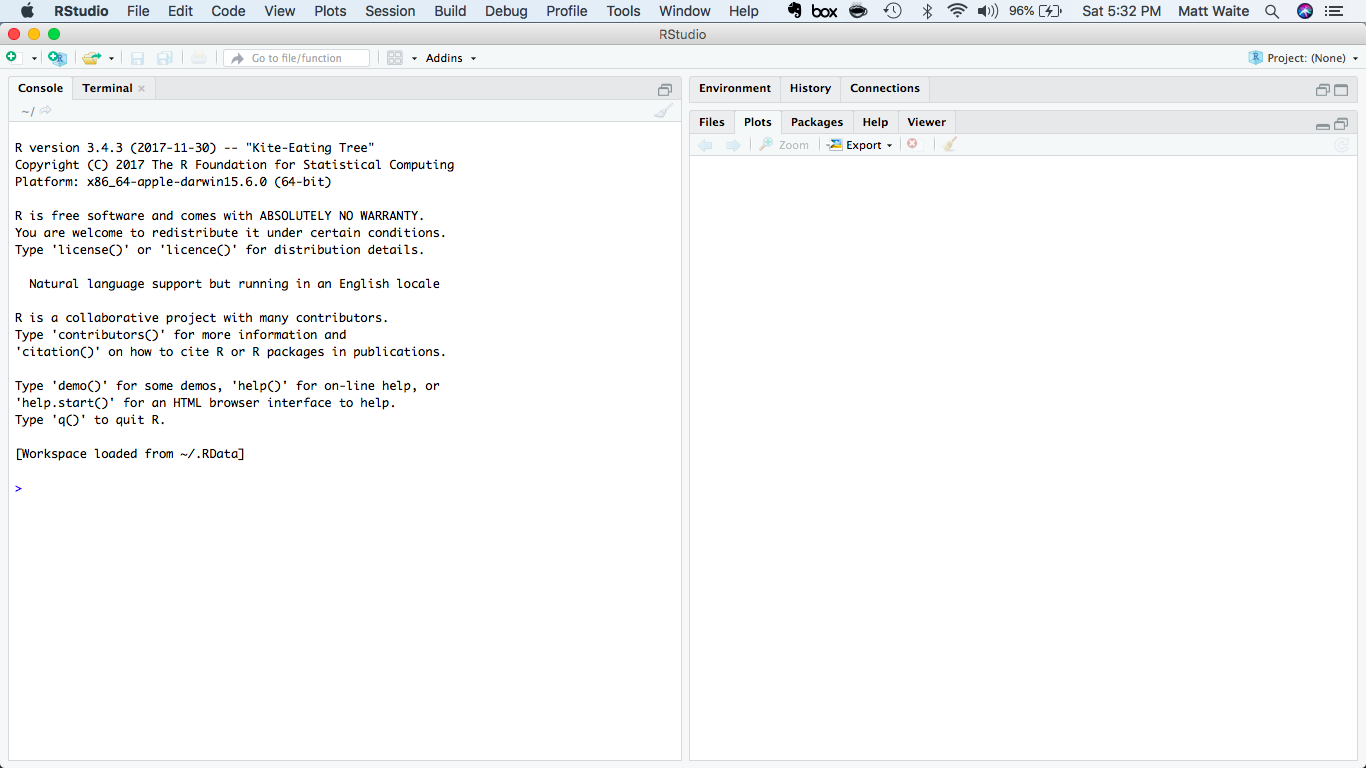
\includegraphics[width=18.97in]{images/verybasics1}

Think of the console like talking directly to R. It's direct, but it has some drawbacks and some quirks we'll get into later. For now, try typing this into the console and hit enter:

\begin{Shaded}
\begin{Highlighting}[]
\DecValTok{2}\OperatorTok{+}\DecValTok{2}
\end{Highlighting}
\end{Shaded}

\begin{verbatim}
## [1] 4
\end{verbatim}

Congrats, you've run some code. It's not very complex, and you knew the answer before hand, but you get the idea. We can compute things. We can also store things. \textbf{In programming languages, these are called variables}. We can assign things to variables using \texttt{\textless{}-}. And then we can do things with them. \textbf{The \texttt{\textless{}-} is a called an assignment operator}.

Try this in your console.

\begin{Shaded}
\begin{Highlighting}[]
\NormalTok{number <-}\StringTok{ }\DecValTok{2}

\NormalTok{number }\OperatorTok{*}\StringTok{ }\NormalTok{number}
\end{Highlighting}
\end{Shaded}

\begin{verbatim}
## [1] 4
\end{verbatim}

Now assign a different number to the variable number. Try run \texttt{number\ *\ number} again. Get what you expected?

We can have as many variables as we can name. \textbf{We can even reuse them (but be careful you know you're doing that or you'll introduce errors)}. Try this in your console.

\begin{Shaded}
\begin{Highlighting}[]
\NormalTok{firstnumber <-}\StringTok{ }\DecValTok{1}
\NormalTok{secondnumber <-}\StringTok{ }\DecValTok{2} 

\NormalTok{(firstnumber }\OperatorTok{+}\StringTok{ }\NormalTok{secondnumber) }\OperatorTok{*}\StringTok{ }\NormalTok{secondnumber}
\end{Highlighting}
\end{Shaded}

\begin{verbatim}
## [1] 6
\end{verbatim}

\textbf{We can store anything in a variable}. A whole table. An array of numbers. A single word. A whole book. All the books of the 18th century. They're really powerful. We'll explore them at length.

\hypertarget{adding-libraries-part-1}{%
\section{Adding libraries, part 1}\label{adding-libraries-part-1}}

The real strength of any given programming language is the external libraries that power it. The base language can do a lot, but it's the external libraries that solve many specific problems -- even making the base language easier to use.

For this class, we're going to need several external libraries.

The first library we're going to use is called Swirl. So in the console, type \texttt{install.packages(\textquotesingle{}swirl\textquotesingle{})} and hit enter. That installs swirl.

Now, to use the library, type \texttt{library(swirl)} and hit enter. That loads swirl. Then type \texttt{swirl()} and hit enter. Now you're running swirl. Follow the directions on the screen. When you are asked, you want to install course 1 R Programming: The basics of programming in R. Then, when asked, you want to do option 1, R Programming, in that course.

When you are finished with the course -- it will take just a few minutes -- type 0 to exit (it will not be clear that's what you do when you are done).

\hypertarget{adding-libraries-part-2}{%
\section{Adding libraries, part 2}\label{adding-libraries-part-2}}

We'll mostly use two libraries for analysis -- \texttt{dplyr} and \texttt{ggplot2}. To get them, and several other useful libraries, we can install a single collection of libraries called the tidyverse. Type this into your console: \texttt{install.packages(\textquotesingle{}tidyverse\textquotesingle{})}

\textbf{NOTE}: This is a pattern. You should always install libraries in the console.

Then, to help us with learning and replication, we're going to use R Notebooks. So we need to install that library. Type this into your console: \texttt{install.packages(\textquotesingle{}rmarkdown\textquotesingle{})}

\hypertarget{data-journalism-in-the-age-of-replication}{%
\chapter{Data journalism in the age of replication}\label{data-journalism-in-the-age-of-replication}}

It's a single word in a single job description, but a Buzzfeed job posting in 2017 is another indicator in what could be a profound shift in how data journalism is both practiced and taught.

``We're looking for someone with a passion for news and a commitment to using data to find amazing, important stories --- both quick hits and deeper analyses that drive conversations,'' the posting seeking a data journalist says. It goes on to list five things BuzzFeed is looking for: Excellent collaborator, clear writer, deep statistical understanding, knowledge of obtaining and restructuring data.

And then there's this:

\textbf{``You should have a strong command of at least one toolset that (a) allows for filtering, joining, pivoting, and aggregating tabular data, and (b) enables reproducible workflows.''}

The word you're seeing more and more of? Reproducible. And it started in earnest this summer when data journalism crossed a major threshold in American journalism: It now has it's own section in the Associated Press Stylebook.

``Data journalism has become a staple of reporting across beats and platforms,'' the Data Journalism section of the Stylebook opens. ``The ability to analyze quantitative information and present conclusions in an engaging and accurate way is no longer the domain of specialists alone.''

The AP's Data Journalism section discusses how to request data and in what format, guidelines for scraping data from websites with automation, the ethics of using leaked or hacked data and other topics long part of data journalism conference talks.

But the third page of the section contains perhaps the most profound commandment: \textbf{``As a general rule, all assertions in a story based on data analysis should be reproducible. The methodology description in the story or accompanying materials should provide a road map to replicate the analysis.''}

Reproducible research -- replication -- is a cornerstone of scientific inquiry. Researchers across a range of academic disciplines use methods to find new knowledge and publish it in peer reviewed journals. And, when it works, other researchers take that knowledge and try it with their own samples in their own locations. Replication studies exist to take something from an Interesting Finding to a Theory and beyond.

It doesn't always work.

Replication studies aren't funded at nearly the level as new research. And, to the alarm of many, scores of studies can't be replicated by others. Researchers across disciplines are finding that when their original studies are replicated, flaws are found, or the effects found aren't as strong as the original. Because of this, academics across a number of disciplines have written about a replication crisis in their respective fields, particularly psychology, social science and medical research.

In Chapter 1 of the New Precision Journalism, Phil Meyer wrote that ``we journalists would be wrong less often if we adapted to our own use some of the research tools of the social scientists.''

Meyer would go on to write about how computers pouring over datasets too large to crunch by hand had changed social science from a discipline with ``a few data and a lot of interpretation'' into a much more meaningful and powerful area of study. If journalists could become comfortable with data and some basic statistics, they too could harness this power.

``It used to be said that journalism is history in a hurry,'' Meyer wrote. ``The argument of this book is that to cope with the acceleration of social change in today's world, journalism must become social science in a hurry.''

He wrote that in 1971. It might as well have been yesterday.

Journalism doesn't have a history of replication, but the concerns about credibility are substantially greater. Trust in media is at an all time low and shows no signs of improving. While the politics of the day have quite a bit to do with this mistrust of media, being more transparent about what journalists do can't hurt.

The AP's commandment that Thou Must Replicate Your Findings could, if taken seriously by the news business, have substantial impacts on how data journalism gets done in newsrooms and how data journalism gets taught, both at professional conferences and universities.

How? Two ways.

\begin{itemize}
\tightlist
\item
  The predominant way that data journalism gets done in a newsroom is through simple tools like Microsoft Excel or Google Sheets. Those simple tools, on their own, lack significant logging functions, meaning journalists will have to maintain detailed logs of what they did so any analysis can be replicated.
\item
  The predominant way that data journalism gets taught -- both in professional settings and at most universities -- doesn't deal with replication at all. The tools and the training stress Getting Things Done -- an entirely logical focus for a deadline driven business. The choices of tools -- like spreadsheets -- are made to get from data to story as quick as possible, without frightening away math and tech phobic students.
\end{itemize}

If the AP's replication rules are to be followed, journalism needs to become much more serious about the tools and techniques used to do data journalism. The days of Point and Click tools to do Quick and Dirty analysis that get published are dying. The days of formal methods using documented steps are here.

\hypertarget{the-stylebook}{%
\section{The stylebook}\label{the-stylebook}}

Troy Thibodeaux, the editor of the AP's data journalism team, said the stylebook entry started when the data team found themselves answering the same questions over and over. With a grant from the Knight Foundation, the team began to document their own standards and turn that into a stylebook section.

From the beginning, they had a fairly clear idea of what they wanted to do -- think through a project and ask what the frequently asked questions are that came up. It was not going to be a soup-to-nuts guide to how to do a data project.

When the section came out, eyebrows went up on the replication parts, surprising Thibodeaux.

``From our perspective, this is a core value for us,'' he said. ``Just for our own benefit, we need to be able to have someone give us a second set of eyes. We benefit from that every day. We catch things for each other.''

Thibodeaux said the AP data team has two audiences when it comes to replication -- they have the readers of the work, and members of the collective who may want to do their own work with the data.

``This is something that's essential to the way we work,'' he said. ``And it's important in terms of transparency and credibility going forward. We thought it would be kind of unexceptionable.''

\hypertarget{replication}{%
\section{Replication}\label{replication}}

Meyer, now 86, said he's delighted to see replication up for discussion now, but warned that we shouldn't take it too far.

``Making the analysis replicable was something I worried about from the very beginning,'' he wrote in an email. So much so that in 1967, after publishing stories from his landmark survey after the Detroit riots, he shipped the data and backup materials about it to a social science data repository at the University of North Carolina.

And, in doing so, he opened the door to others replicating his results. One scholar attempted to find fault with Meyer's analysis by slicing the data ever thinner until the differences weren't significant -- gaming the analysis to criticize the stories.

Meyer believes replication is vitally important, but doesn't believe it should take on the trappings of science replication, where newsrooms take their own samples or re-survey a community. That would be prohibitively expensive.

But journalists should be sharing their data and analysis steps. And it doesn't need to be complicated, he said.

``Replication is a theoretical standard, not a requirement that every investigator duplicate his or her own work for every project,'' he said. ``Giving enough information in the report to enable another investigator to follow in your footsteps is enough. Just telling enough to make replication possible will build confidence.''

But as simple as that sounds, it's not so simple. Ask social scientists.

Andrew Gelman, a professor of statistics and political science and director of the Applied Statistics Center at Columbia University, wrote in the journal CHANCE in February that difficulties with replication in empirical research are pervasive.

``When an outsider requests data from a published paper, the authors will typically not post or send their data files and code, but instead will point to their sources, so replicators have to figure out exactly what to do from there,'' Gelman wrote. ``End-to-end replicability is not the norm, even among scholars who actively advocate for the principles of open science.''

So goes science, so goes journalism.

Until a recent set of exceptions, journalists rarely shared data. The ``nerd box'' -- a sidebar story that explains how a news organization did what they did -- is a term that first appeared on NICAR-L, a email listserv of data journalists, in the 1990s.

It was a form born in print.

As newsrooms adapted to the internet, some news organizations began linking to their data sources if they were online. Often, the data used in stories were obtained through records requests. Sometimes, reporters created the data themselves.

Journalism, more explicitly than science, is a competitive business. There have been arguments that nerd boxes and downloadable links give too much away to competitors.

Enter the AP Stylebook.

The AP Stylebook argues explicitly for both internal and external replication. Externally, they argue that the \textbf{``methodology description in the story or accompanying materials should provide a road map to replicate the analysis''}, meaning someone else could do the replication post publication.

Internally, the AP Stylebook says: \textbf{``If at all possible, an editor or another reporter should attempt to reproduce the results of the analysis and confirm all findings before publication.''}

There are two problems here.

First is that journalism, unlike science, has no history of replication. There is no Scientific Method for stories. There is no Research Methods class taught at every journalism school, at least not where it comes to writing stories. And, beyond that, journalism school isn't a requirement to get into the news business. In other words, journalism lacks the standards other disciplines have.

The second problem is, in many ways, worse: Except for the largest newsrooms, most news organizations lack editors who could replicate the analysis. Many don't have a second person who would know what to do.

Not having a second set of eyes in a newsroom is a problem, Thibodeaux acknowledges. Having a data journalism team ``is an incredible luxury'' at the AP, he said, and their rule is nothing goes on the wire without a second set of eyes.

Thibodeaux, for his part, wants to see fewer ``lone nerds in the corner'' -- it's too much pressure. That person gets too much credibility from people who don't understand what they do, and they get too much blame when a mistake is made.

So what would replication look like in a newsroom? What does this mean for how newsrooms do data journalism on deadline? And what does this mean for how data journalism is being taught, particularly at a time when only half of accredited journalism programs teach any data journalism at all?

Are we walking ourselves into our own replication crisis?

\hypertarget{goodbye-excel}{%
\section{Goodbye Excel?}\label{goodbye-excel}}

For decades, Excel has been the gateway drug for data journalists, the Swiss Army knife of data tools, the One Tool You Can't Live Without. Investigative Reporters and Editors, an organization that trains investigative journalists, have built large amounts of their curricula around Excel. Of the journalism schools that teach data journalism, most of them begin and end with spreadsheets.

The Stylebook says at a minimum, today's data journalists should keep a log that details:

\begin{itemize}
\tightlist
\item
  The source of the data, making sure to work on a copy of the data and not the original file.
\item
  Data dictionaries or any other supporting documentation of the data.
\item
  \textbf{``Description of all steps required to transform the data and perform the analysis.''}
\end{itemize}

The trouble with Excel is, unless you are keeping meticulous notes on what steps you are taking, there's no way to keep track. Many data journalists will copy and paste the values of a formula over the formula itself to prevent Excel from fouling up cell references when moving data around -- a practical step that also cuts off another path to being able to replicate the results.

An increasing number of data journalists are switching to tools like analysis notebooks, which use languages like Python and R, to document their work. The notebooks, generally speaking, allow a data journalist to mix code and explanation in the same document.

Combined with online sharing tools like GitHub, analysis notebooks seem to solve the problem of replication. But the number using them is small compared to those using spreadsheets. Recent examples of news organizations using analysis notebooks include the \href{https://github.com/datadesk}{Los Angeles Times}, the \href{https://github.com/TheUpshot}{New York Times}, \href{https://github.com/fivethirtyeight/data}{FiveThirtyEight}, and \href{https://github.com/BuzzFeedNews}{Buzzfeed}.

Peter Aldous, a data journalist at Buzzfeed recently published a story about how the online news site used machine learning to find airplanes being used to spy on people in American cities. Published with the story is the code Aldous used to build his case.

``I think of it this way: As a journalist, I don't like to simply trust what people tell me. Sometimes sources lie. Sometimes they're just mistaken. So I like to verify what I'm told,'' he wrote in an email. ``By the same token, why should someone reading one of my articles believe my conclusions, if I don't provide the evidence that explains how I reached them?''

The methodology document, associated code and source data took Aldous a few hours to create. The story, from the initial data work through the reporting required to make sense of it all, took a year. Aldous said there wasn't a discussion about if the methodology would be published because it was assumed -- ``it's written into our DNA at BuzzFeed News.''

``My background is in science journalism, and before that (way back in the 1980s) in science,'' Aldous said. ``In science, there's been a shift from descriptive methods sections to publishing data and analysis code for reproducible research. And I think we're seeing a similar shift in data journalism. Simply saying what you've done is not as powerful as providing the means for others to repeat and build on your work.''

Thibodeaux said that what Buzzfeed and others do with analysis notebooks and code repositories that include their data is ``lovely.''

``That to me is the shining city on the hill,'' Thibodeaux said. ``We're not going to get there, and I don't think we have to for every story and every use case, and I don't think it's necessarily practical for every person working with data to get to that point.''

There's a wide spectrum of approaches that still gets journalists to the essence of what the stylebook is trying to do, Thibodeaux said. There are many tools, many strategies, and the AP isn't going to advocate for any single one of them, he said. They're just arguing for transparency and replicability, even if that means doing more work.

``There's a certain burden that comes with transparency,'' he said. ``And I think we have to accept that burden.''

The question, Thibodeaux said, is what is sufficient? What's enough transparency? What does someone need for replicability?

``Maybe we do have to set a higher standard -- the more critical the analysis is to the story, and the more complex that analysis is, that's going to push the bar on what is a sufficient methodology statement,'' he said. ``And it could end up being a whole code repo in order to just say, this isn't black magic, here's how we got it if you're so interested.''

\hypertarget{receptivity-is-high}{%
\section{``Receptivity \ldots{} is high''}\label{receptivity-is-high}}

Though written almost half a century ago, Meyer foresaw how data journalism was going to arrive in the newsroom.

``For the new methods to gain currency in journalism, two things must happen,'' he wrote. ``Editors must feel the need strongly enough to develop the in-house capacity for systematic research \ldots{} The second need, of course, is for the editors to be able to find the talent to fill this need.''

Meyer optimistically wrote that journalism schools were prepared to provide that talent -- they were not then, and only small handful are now -- but students were unlikely to be drawn to these new skills if they didn't see a chance to use those skills in their careers.

It's taken 45 years, but we are now at this point.

``The potential for receptivity, especially among the younger generation of newspaper managers, is high,'' Meyer wrote.

\hypertarget{replication-in-notebooks}{%
\section{Replication in notebooks}\label{replication-in-notebooks}}

For our purposes in this book, replication requires two things from you, the student: What and why. What is this piece of code doing, and why are you doing that here and now? What lead you to this place? That you can copy and paste code from this book or the internet is not impressive. What is necessary for learning is that you know what a piece of code is doing a thing and why you want to do that thing here.

In an R Notebook, there are two blocks: A block that uses markdown, which has no special notation, and a code block. The code blocks can run mulitple languages inside R Studio, including Python, a general purpose scripting language; and SQL, or Structured Query Language, the language of databases.

For the rest of the class, we're going to be working in notebooks. In notebooks, you will both run your code and explain each step, much as I am doing here.

To start a notebook, you click on the green plus in the top left corner and go down to R Notebook. Do that now.

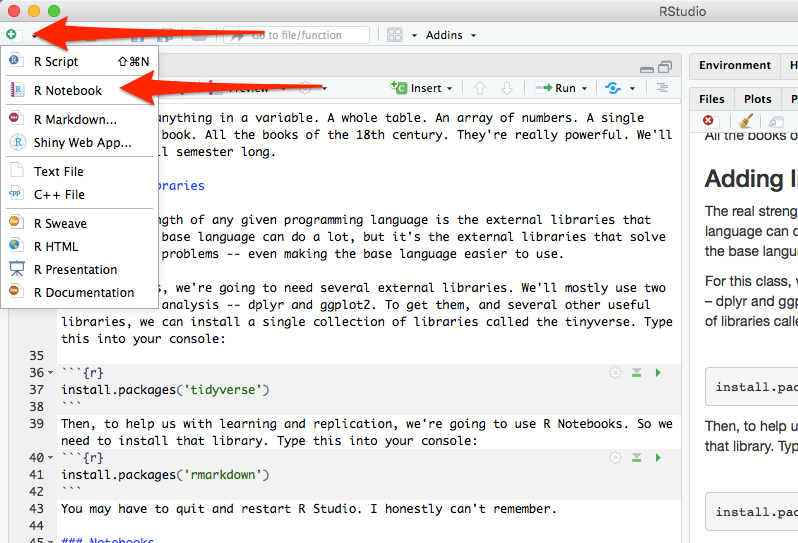
\includegraphics[width=11.08in]{images/verybasics2}

You will see that the notebook adds a lot of text for you. It tells you how to work in notebooks -- and you should read it. The most important parts are these:

To add text, simply type. To add code you can click on the \emph{Insert} button on the toolbar or by pressing \emph{Cmd+Option+I} on Mac or \emph{Ctl+Alt+I} on Windows.

Highlight all that text and delete it. You should have a blank document. This document is called a R Markdown file -- it's a special form of text, one that you can style, and one you can include R in the middle of it. Markdown is a simple markup format that you can use to create documents. So first things first, let's give our notebook a big headline. Add this:

\texttt{\#\ My\ awesome\ notebook}

Now, under that, without any markup, just type This is my awesome notebook.

Under that, you can make text bold by writing \texttt{It\ is\ **really**\ awesome}.

If you want it italics, just do this on the next line: \texttt{No,\ it\textquotesingle{}s\ \_really\_\ awesome.\ I\ swear.}

To see what it looks like without the markup, click the Preview or Knit button in the toolbar. That will turn your notebook into a webpage, with the formatting included.

Throughout this book, we're going to use this markdown to explain what we are doing and, more importantly, why we are doing it. Explaining your thinking is a vital part of understanding what you are doing.

That explaination, plus the code, is the real power of notebooks. To add a block of code, follow the instructions from above: click on the \emph{Insert} button on the toolbar or by pressing \emph{Cmd+Option+I} on Mac or \emph{Ctl+Alt+I} on Windows.

In that window, use some of the code from above and add two numbers together. To see it run, click the green triangle on the right. That runs the chunk. You should see the answer to your addition problem.

And that, just that, is the foundation you need to start this book.

\hypertarget{data-structures-and-types}{%
\chapter{Data, structures and types}\label{data-structures-and-types}}

Data are everywhere (and data is plural of datum, thus the use of are in that statement). It surrounds you. Every time you use your phone, you are creating data. Lots of it. Your online life. Any time you buy something. It's everywhere. News, like life, is no different. Modernity is drowning in data, and more comes along all the time.

In news, and in this class, we'll be dealing largely with two kinds of data: \textbf{event level data and summary data}. It's not hard to envision event level data. A car accident. A crime. A fire. They are the events that make up the whole. Combine them together -- summarize them -- and you'll have some notion of how the year went. What we usually see is summary data -- who wants to scroll through 365 days of crime data to figure out if crime was up or down?

To start with, we need to understand the shape of data.

\hypertarget{rows-and-columns}{%
\section{Rows and columns}\label{rows-and-columns}}

Data, oversimplifying it a bit, is information organized. Generally speaking, it's organized into rows and columns. Rows, generally, are individual elements. A crime. A county. An accident. Columns, generally, are components of the data, sometimes called variables. So if each row is a crime, the first column might be the type. The second is the date and time. The third is the location. And so on.

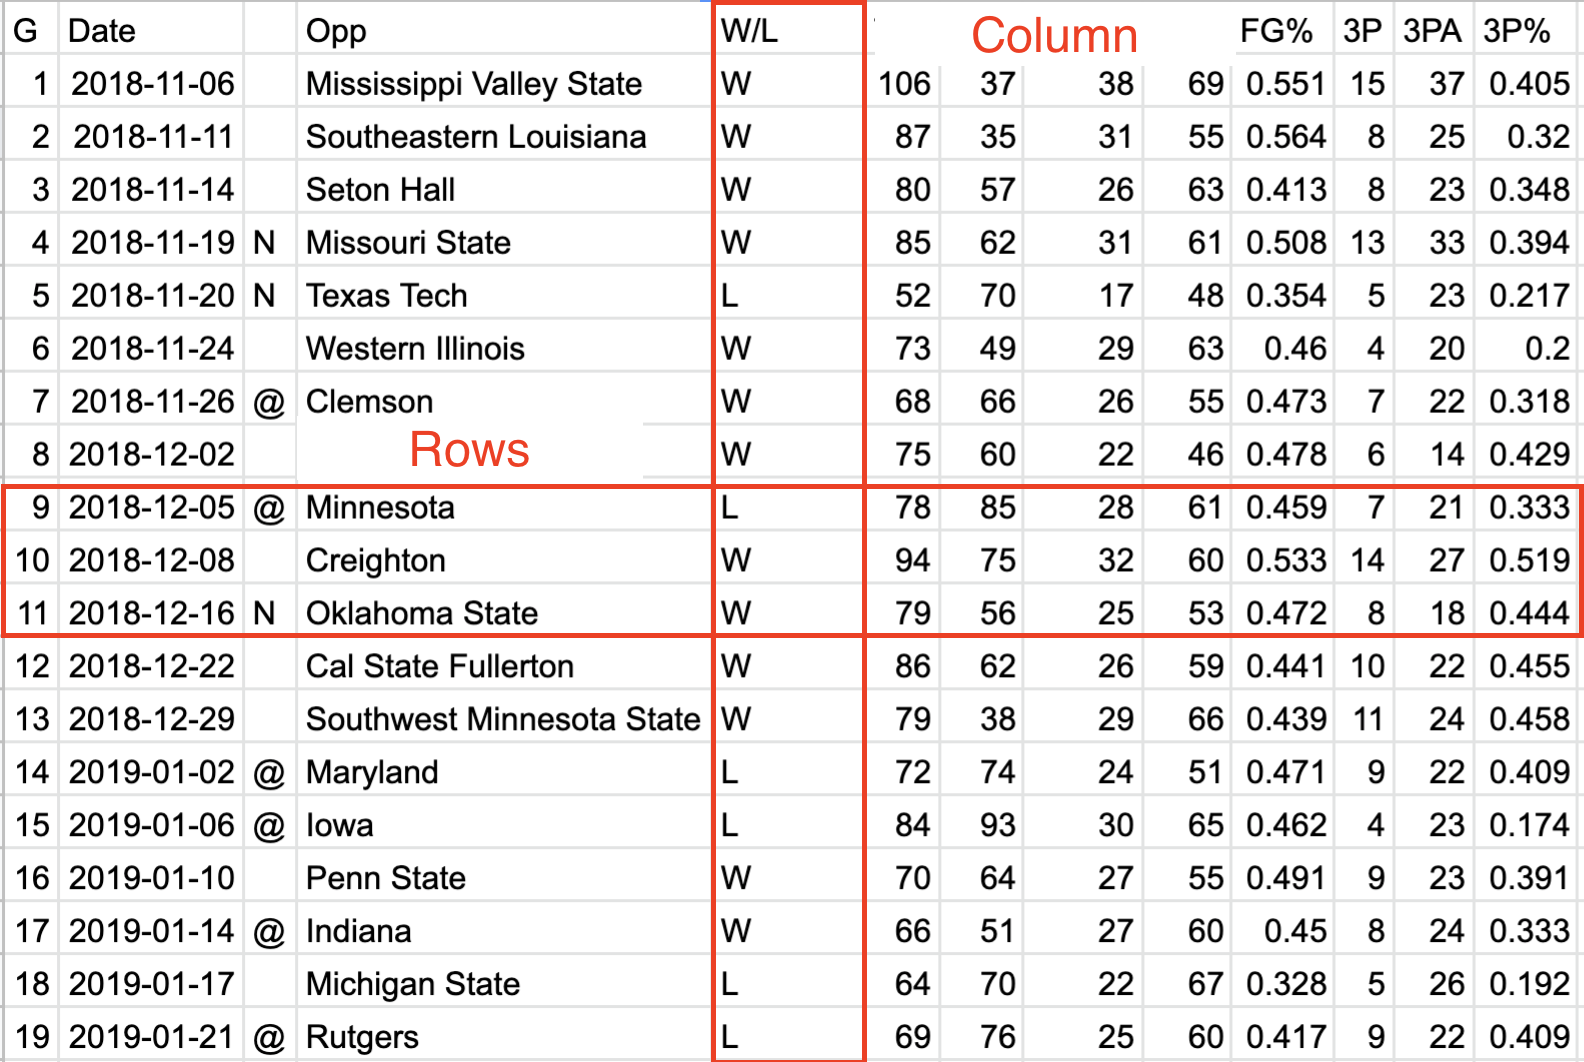
\includegraphics[width=22in]{images/data1}

One of the critical components of data analysis, especially for beginners, is having a mental picture of your data. What does each row mean? What does each column in each row signify? How many rows do you have? How many columns?

\begin{quote}
EXERCISE: I love orange Skittles. What are my chances of getting more orange Skittles than other colors in a fun sized packet? Each person in the class must track their package and everyone else using a spreadsheet. What differences between sheets emerge? What similarities?
\end{quote}

\hypertarget{types}{%
\section{Types}\label{types}}

There are scores of data types in the world, and R has them. In this class, we're primarily going to be dealing with data frames, and each element of our data frames will have a data type.

Typically, they'll be one of four types of data:

\begin{itemize}
\tightlist
\item
  Numeric: a number, like the number of car accidents in a year or the number of journalism majors.
\item
  Character: Text, like a name, a county, a state.
\item
  Date: Fully formed dates -- 2019-01-01 -- have a special date type. Elements of a date, like a year (ex. 2019) are not technically dates, so they'll appear as numeric data types.
\item
  Logical: Rare(ish), but every now and then we'll have a data type that's Yes or No, True or False, etc.
\end{itemize}

\textbf{Question:} Is a zip code a number? Is a jersey number a number? Trick question, because the answer is no. Numbers are things we do math on. If the thing you want is not something you're going to do math on -- can you add two phone numbers together? -- then make it a character type. If you don't, most every software system on the planet will drop leading zeros. For example, every zip code in Boston starts with 0. If you record that as a number, your zip code will become a four digit number, which isn't a zip code anymore.

\hypertarget{a-simple-way-to-get-data}{%
\section{A simple way to get data}\label{a-simple-way-to-get-data}}

The hardest part of doing data journalism is often getting the data. In news, there's scores of organizations and agencies collecting data, and zero standards on how it's being collected.

If we're lucky -- huge IF in news -- the data we want is in a downloadable format. If we're a little less lucky, there's a way to get the data on the web. And maybe that data is in a simple table. If so, we can pull that data directly into Google Sheets.

The Lincoln Police Department publishes a daily summary of calls. Some days -- like when it snows -- that data becomes news. So let's pretend that it snowed today and we need to see how many accidents the Lincoln Police responded to and what percentage of their call load that represents.

Open a browser and go to the \href{http://cjis.lincoln.ne.gov/~lpd/cfstoday.htm}{LPD's log page}. Now, in a new tab, log into Google Docs/Drive and open a new spreadsheet. In the first cell of the first row, copy and paste this formula in:

\begin{verbatim}
=importHTML("http://cjis.lincoln.ne.gov/~lpd/cfstoday.htm","table",1)
\end{verbatim}

This is \textbf{function}, with three \textbf{inputs}. The function is \texttt{importHTML} and the three inputs in order are the url of the page, the HTML tag we're after (a

tag in our case) and the number of the tag you're after. So our function says go to the LPD page and get the first table tag you find. Fortunately for us, there's only one.

If your version worked right, you've got the data from that page in a spreadsheet.

\hypertarget{cleaning-the-data}{%
\section{Cleaning the data}\label{cleaning-the-data}}

The first thing we need to do is recognize that we don't have data, really. We have the results of a formula. You can tell by putting your cursor on that field, where you'll see the formula again. This is where you'd look:

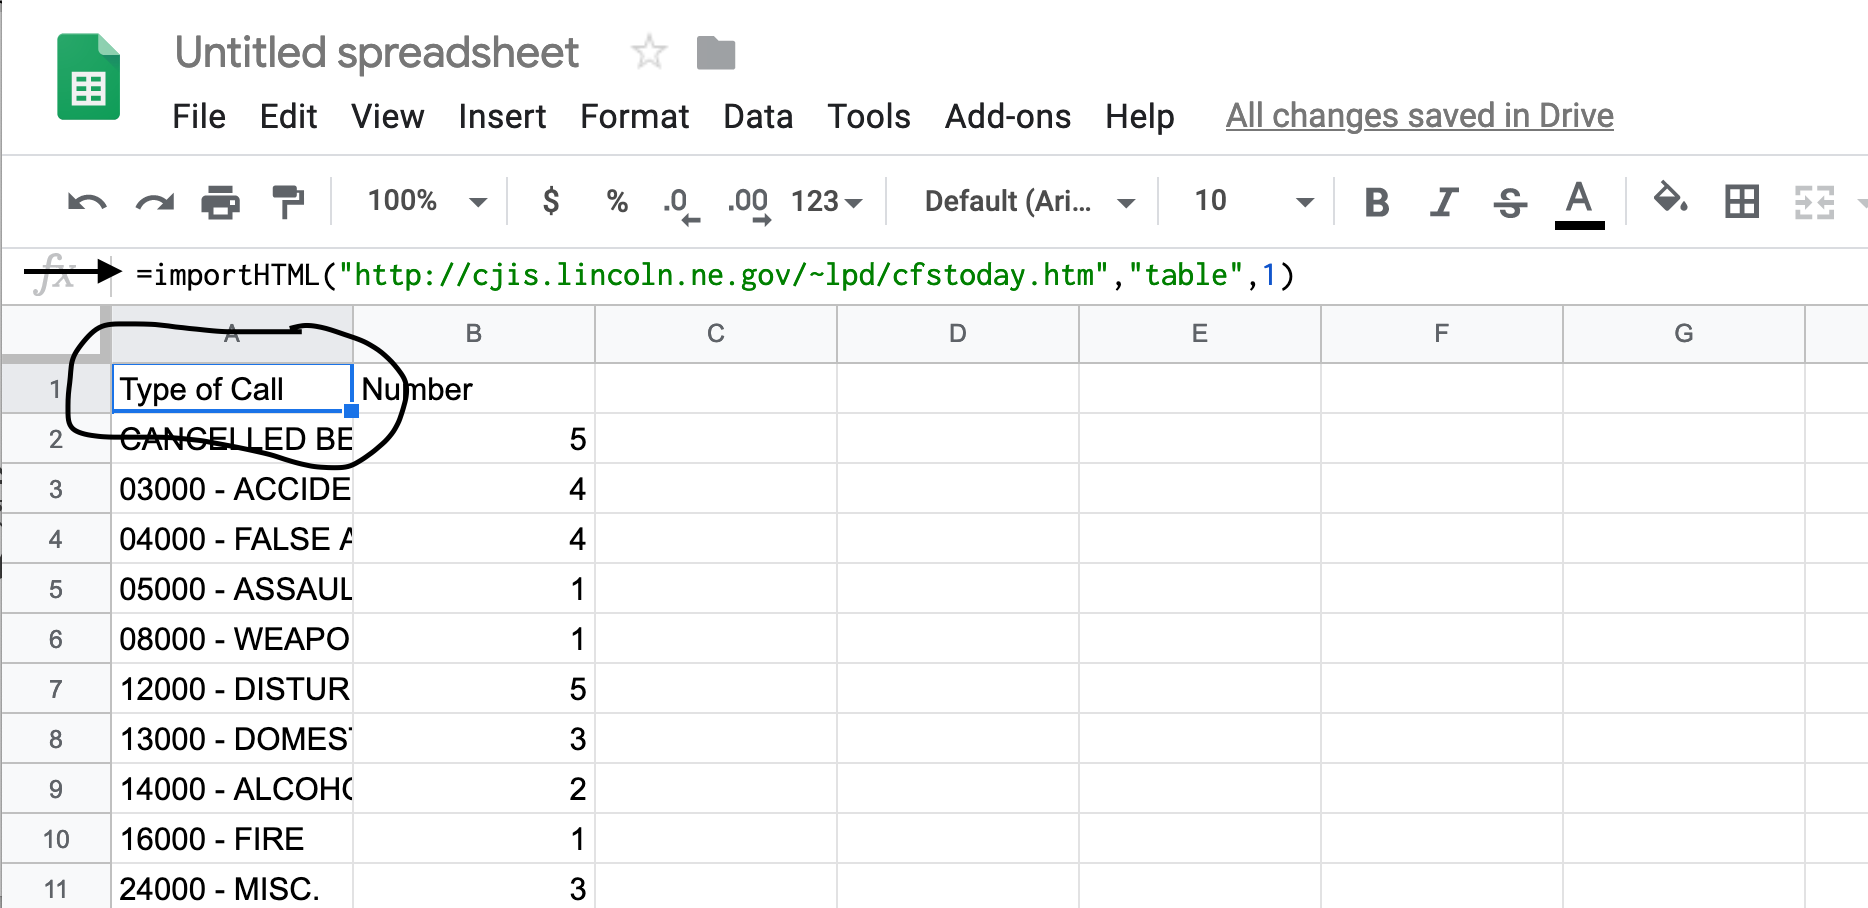
\includegraphics[width=25.94in]{images/clean1}

The solution is easy:

Edit \textgreater{} Select All or type command/control A
Edit \textgreater{} Copy or type command/control C
Edit \textgreater{} Paste Special \textgreater{} Values Only or type command/control shift V

You can verify that it worked by looking in that same row 1 column A, where you'll see the formula is gone.

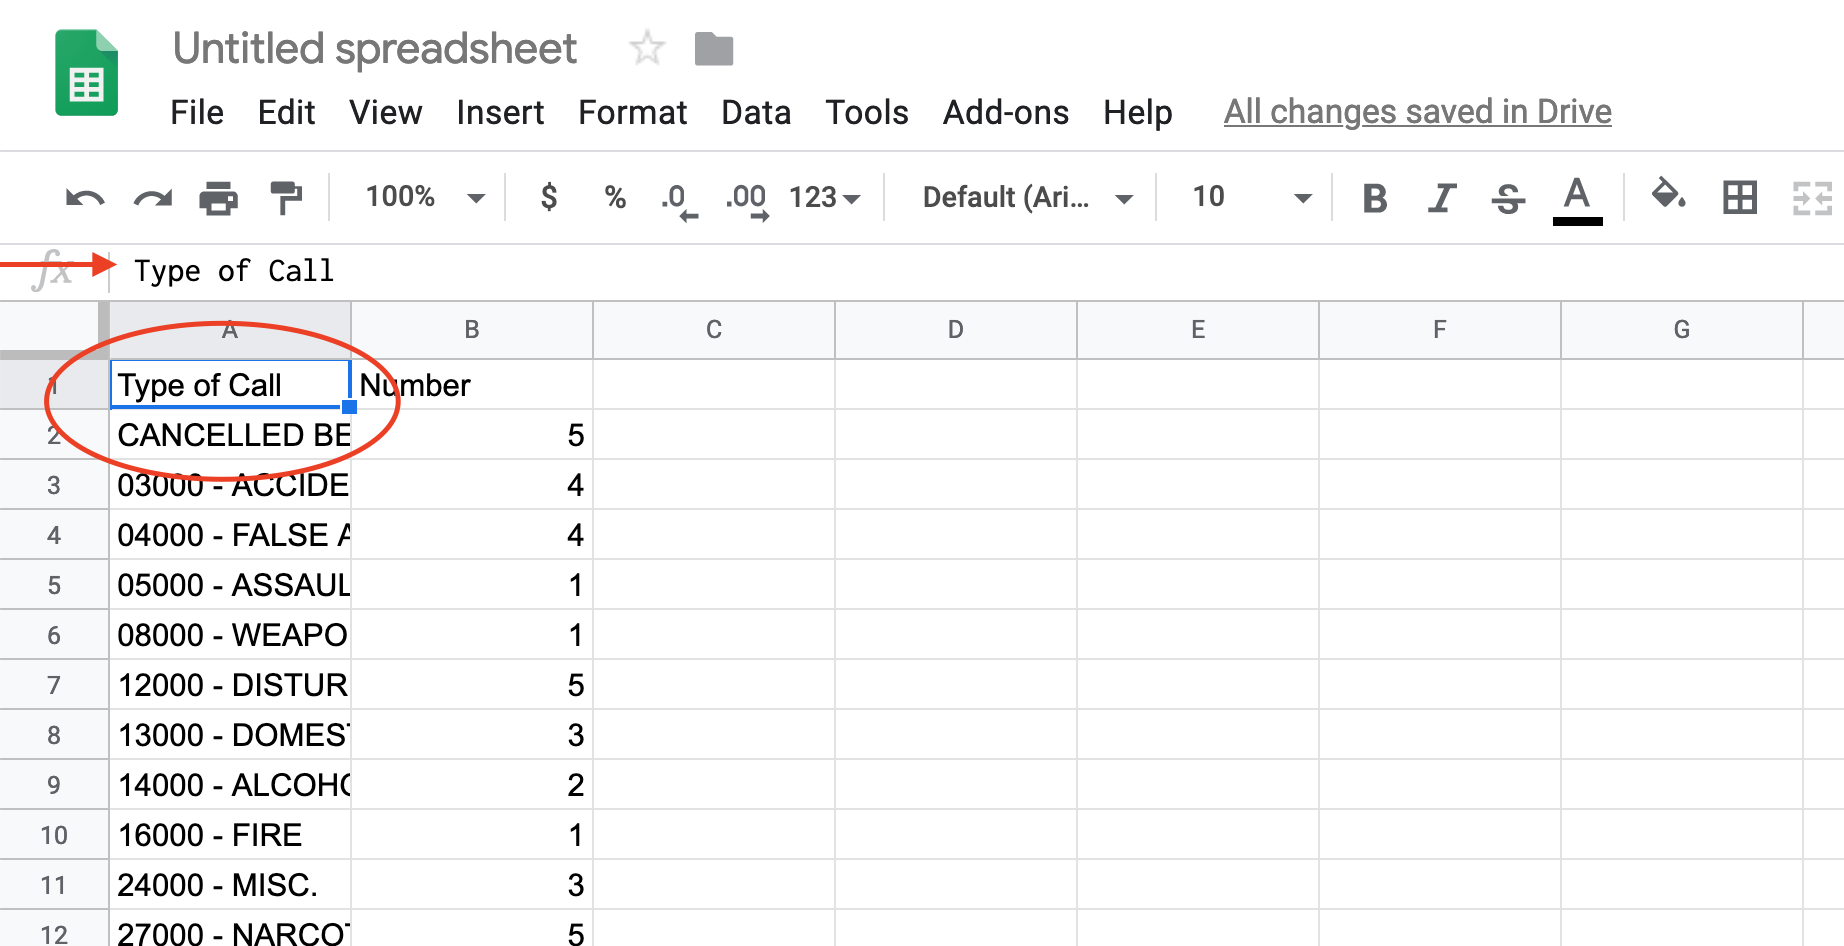
\includegraphics[width=25.61in]{images/clean2}

Now you have data, but look closely. At the bottom of the data, you have the total number of calls. More often than not, and particularly the deeper into this book we go, you want to delete that. So click on the number next to that Total Calls line to highlight it and go up to Edit \textgreater{} Delete Row XX where XX is the row number.

After you've done that, you can export it for use in R. Go to File \textgreater{} Download as \textgreater{} Comma Separated Values.

\hypertarget{aggregates}{%
\chapter{Aggregates}\label{aggregates}}

R is a statistical programming language that is purpose built for data analysis.

Base R does a lot, but there are a mountain of external libraries that do things to make R better/easier/more fully featured. We already installed the tidyverse -- or you should have if you followed the instructions for the last assignment -- which isn't exactly a library, but a collection of libraries. Together, they make up the tidyverse. Individually, they are extraordinarily useful for what they do. We can load them all at once using the tidyverse name, or we can load them individually. Let's start with individually.

The two libraries we are going to need for this assignment are \texttt{readr} and \texttt{dplyr}. The library \texttt{readr} reads different types of data in. For this assignment, we're going to read in csv data or Comma Separated Values data. That's data that has a comma between each column of data.

Then we're going to use \texttt{dplyr} to analyze it.

To use a library, you need to import it. Good practice -- one I'm going to insist on -- is that you put all your library steps at the top of your notebooks.

That code looks like this:

\begin{Shaded}
\begin{Highlighting}[]
\KeywordTok{library}\NormalTok{(readr)}
\end{Highlighting}
\end{Shaded}

To load them both, you need to do this:

\begin{Shaded}
\begin{Highlighting}[]
\KeywordTok{library}\NormalTok{(readr)}
\KeywordTok{library}\NormalTok{(dplyr)}
\end{Highlighting}
\end{Shaded}

But, because those two libraries -- and several others that we're going to use over the course of this class -- are so commonly used, there's a shortcut to loading all of the libraries we'll need:

\begin{Shaded}
\begin{Highlighting}[]
\KeywordTok{library}\NormalTok{(tidyverse)}
\end{Highlighting}
\end{Shaded}

You can keep doing that for as many libraries as you need. I've seen notebooks with 10 or more library imports.

\hypertarget{importing-data}{%
\section{Importing data}\label{importing-data}}

The first thing we need to do is get some data to work with. We do that by reading it in. In our case, we're going to read data from a csv file -- a comma-separated values file.

The CSV file we're going to read from is a \href{https://unl.box.com/s/xjipgkesl9rjmng4weg77vb73xt41apf}{Nebraska Game and Parks Commission dataset} of confirmed mountain lion sightings in Nebraska. There are, on occasion, fierce debates about mountain lions and if they should be hunted in Nebraska. This dataset can tell us some interesting things about that debate.

So step 1 is to import the data. The code looks \emph{something} like this, but hold off copying it just yet:

\texttt{mountainlions\ \textless{}-\ read\_csv("\textasciitilde{}/Documents/Data/mountainlions.csv")}

Let's unpack that.

The first part -- mountainlions -- is the name of your variable. A variable is just a name of a thing. In this case, our variable is a dataframe, which is R's way of storing data. We can call this whatever we want. I always want to name dataframes after what is in it. In this case, we're going to import a dataset of mountain lion sightings from the Nebraska Game and Parks Commission. \textbf{Variable names, by convention are one word all lower case}. You can end a variable with a number, but you can't start one with a number.

The \textless{}- bit, you'll recall from the basics, is the \textbf{variable assignment operator}. It's how we know we're assigning something to a word. Think of the arrow as saying ``Take everything on the right of this arrow and stuff it into the thing on the left.'' So we're creating an empty vessel called mountainlions and stuffing all this data into it.

The \texttt{read\_csv} bits are pretty obvious, except for one thing. What happens in the quote marks is the path to the data. In there, I have to tell R where it will find the data.

\begin{quote}
The easiest thing to do, if you are confused about how to find your data, is to put your data in the same folder as as your notebook (you'll have to save that notebook first). If you do that, then you just need to put the name of the file in there (mountainlions.csv).
\end{quote}

In my case, the file path I've got starts with a \textasciitilde{} character. That's a shortcut for my home directory. It's the same on your computer. Your home directory is where your Documents, Desktop and Downloads directories are. I've got a folder called Documents in my home directory, and in there is a folder called Data that has the file called mountainlions.csv in it. Thus, \texttt{\textasciitilde{}/Documents/Data/mountainlions.csv}

Some people -- insane people -- leave the data in their downloads folder. The data path then would be \texttt{\textasciitilde{}/Downloads/nameofthedatafilehere.csv} on PC or Mac.

A quick way to find your data file? The tab key. If you start your code \texttt{dataframenamehere\ \textless{}-\ read\_csv(")} and after typing the first quote mark you hit tab, it will show you the files in the folder you are in. With that, you can start to narrow in on where you need to go.

\textbf{So what you put in your import step will be different from mine}. Your first task is to import the data. Here's mine. Use the tab key to find your data file and get the correct path.

\begin{Shaded}
\begin{Highlighting}[]
\NormalTok{mountainlions <-}\StringTok{ }\KeywordTok{read_csv}\NormalTok{(}\StringTok{"data/mountainlions.csv"}\NormalTok{)}
\end{Highlighting}
\end{Shaded}

\begin{verbatim}
## Parsed with column specification:
## cols(
##   ID = col_double(),
##   `Cofirm Type` = col_character(),
##   COUNTY = col_character(),
##   Date = col_character()
## )
\end{verbatim}

Now we can inspect the data we imported. What does it look like? To do that, we use \texttt{head(mountainlions)} to \textbf{show the headers and the first six rows of data}. If we wanted to see them all, we could just simply enter \texttt{mountainlions} and run it.

To get the number of records in our dataset, we run \texttt{nrow(mountainlions)}

\begin{Shaded}
\begin{Highlighting}[]
\KeywordTok{head}\NormalTok{(mountainlions)}
\end{Highlighting}
\end{Shaded}

\begin{verbatim}
## # A tibble: 6 x 4
##      ID `Cofirm Type` COUNTY       Date    
##   <dbl> <chr>         <chr>        <chr>   
## 1     1 Track         Dawes        9/14/91 
## 2     2 Mortality     Sioux        11/10/91
## 3     3 Mortality     Scotts Bluff 4/21/96 
## 4     4 Mortality     Sioux        5/9/99  
## 5     5 Mortality     Box Butte    9/29/99 
## 6     6 Track         Scotts Bluff 11/12/99
\end{verbatim}

\begin{Shaded}
\begin{Highlighting}[]
\KeywordTok{nrow}\NormalTok{(mountainlions)}
\end{Highlighting}
\end{Shaded}

\begin{verbatim}
## [1] 393
\end{verbatim}

\hypertarget{group-by-and-count}{%
\section{Group by and count}\label{group-by-and-count}}

So what if we wanted to know how many mountain lion sightings there were in each county?

To do that by hand, we'd have to take each of the 393 records and sort them into a pile. We'd put them in groups and then count them.

\texttt{dplyr} has a group by function in it that does just this. A massive amount of data analysis involves grouping like things together and then doing simple things like counting them, or averaging them together. So it's a good place to start.

So to do this, we'll take our dataset and we'll introduce a new operator: \texttt{\%\textgreater{}\%}. The best way to read that operator, in my opinion, is to interpret that as ``and then do this.''

We're going to establish a pattern that will come up again and again throughout this book: \texttt{data\ \%\textgreater{}\%\ function}. The first step of every analysis starts with the data being used. Then we apply functions to the data.

In our case, the pattern that you'll use many, many times is: \texttt{data\ \%\textgreater{}\%\ group\_by(FIELD\ NAME)\ \%\textgreater{}\%\ summarize(VARIABLE\ NAME\ =\ AGGREGATE\ FUNCTION(FIELD\ NAME))}

Here's the code:

\begin{Shaded}
\begin{Highlighting}[]
\NormalTok{mountainlions }\OperatorTok
\StringTok{  }\KeywordTok{group_by}\NormalTok{(COUNTY) }\OperatorTok
\StringTok{  }\KeywordTok{summarise}\NormalTok{(}
    \DataTypeTok{total =} \KeywordTok{n}\NormalTok{()}
\NormalTok{  )}
\end{Highlighting}
\end{Shaded}

\begin{verbatim}
## # A tibble: 42 x 2
##    COUNTY    total
##    <chr>     <int>
##  1 Banner        6
##  2 Blaine        3
##  3 Box Butte     4
##  4 Brown        15
##  5 Buffalo       3
##  6 Cedar         1
##  7 Cherry       30
##  8 Custer        8
##  9 Dakota        3
## 10 Dawes       111
## # ... with 32 more rows
\end{verbatim}

So let's walk through that. We start with our dataset -- \texttt{mountainlions} -- and then we tell it to group the data by a given field in the data. In this case, we wanted to group together all the counties, signified by the field name COUNTY, which you could get from looking at \texttt{head(mountainlions)}. After we group the data, we need to count them up. In dplyr, we use \texttt{summarize} \href{http://dplyr.tidyverse.org/reference/summarise.html}{which can do more than just count things}. Inside the parentheses in summarize, we set up the summaries we want. In this case, we just want a count of the counties: \texttt{total\ =\ n(),} says create a new field, called \texttt{total} and set it equal to \texttt{n()}, which might look weird, but it's common in stats. The number of things in a dataset? Statisticians call in n. There are n number of incidents in this dataset. So \texttt{n()} is a function that counts the number of things there are.

And when we run that, we get a list of counties with a count next to them. But it's not in any order. So we'll add another And Then Do This \%\textgreater{}\% and use \texttt{arrange}. Arrange does what you think it does -- it arranges data in order. By default, it's in ascending order -- smallest to largest. But if we want to know the county with the most mountain lion sightings, we need to sort it in descending order. That looks like this:

\begin{Shaded}
\begin{Highlighting}[]
\NormalTok{mountainlions }\OperatorTok
\StringTok{  }\KeywordTok{group_by}\NormalTok{(COUNTY) }\OperatorTok
\StringTok{  }\KeywordTok{summarise}\NormalTok{(}
    \DataTypeTok{count =} \KeywordTok{n}\NormalTok{()}
\NormalTok{  ) }\OperatorTok\StringTok{ }\KeywordTok{arrange}\NormalTok{(}\KeywordTok{desc}\NormalTok{(count))}
\end{Highlighting}
\end{Shaded}

\begin{verbatim}
## # A tibble: 42 x 2
##    COUNTY       count
##    <chr>        <int>
##  1 Dawes          111
##  2 Sioux           52
##  3 Sheridan        35
##  4 Cherry          30
##  5 Scotts Bluff    26
##  6 Keya Paha       20
##  7 Brown           15
##  8 Rock            11
##  9 Lincoln         10
## 10 Custer           8
## # ... with 32 more rows
\end{verbatim}

We can, if we want, group by more than one thing. So how are these sightings being confirmed? To do that, we can group by County and ``Cofirm Type'', which is how the state misspelled Confirm. But note something in this example below:

\begin{Shaded}
\begin{Highlighting}[]
\NormalTok{mountainlions }\OperatorTok
\StringTok{  }\KeywordTok{group_by}\NormalTok{(COUNTY, }\StringTok{`}\DataTypeTok{Cofirm Type}\StringTok{`}\NormalTok{) }\OperatorTok
\StringTok{  }\KeywordTok{summarise}\NormalTok{(}
    \DataTypeTok{count =} \KeywordTok{n}\NormalTok{()}
\NormalTok{  ) }\OperatorTok\StringTok{ }\KeywordTok{arrange}\NormalTok{(}\KeywordTok{desc}\NormalTok{(count))}
\end{Highlighting}
\end{Shaded}

\begin{verbatim}
## # A tibble: 93 x 3
## # Groups:   COUNTY [42]
##    COUNTY       `Cofirm Type`      count
##    <chr>        <chr>              <int>
##  1 Dawes        Trail Camera Photo    41
##  2 Sioux        Trail Camera Photo    40
##  3 Dawes        Track                 19
##  4 Keya Paha    Trail Camera Photo    18
##  5 Cherry       Trail Camera Photo    17
##  6 Dawes        Mortality             17
##  7 Sheridan     Trail Camera Photo    16
##  8 Dawes        Photo                 13
##  9 Dawes        DNA                   11
## 10 Scotts Bluff Trail Camera Photo    11
## # ... with 83 more rows
\end{verbatim}

See it? When you have a field name that has two words, \texttt{readr} wraps it in back ticks, which is next to the 1 key on your keyboard. You can figure out which fields have back ticks around it by looking at the output of \texttt{readr}. Pay attention to that, because it's coming up again in the next section and will be a part of your homework.

\hypertarget{other-aggregates-mean-and-median}{%
\section{Other aggregates: Mean and median}\label{other-aggregates-mean-and-median}}

In the last example, we grouped some data together and counted it up, but there's so much more you can do. You can do multiple measures in a single step as well.

Let's look at some \href{https://unl.box.com/s/09t2u4qoncfh6qlv2156flzlxb8ruzpq}{salary data from the University of Nebraska}.

\begin{Shaded}
\begin{Highlighting}[]
\NormalTok{salaries <-}\StringTok{ }\KeywordTok{read_csv}\NormalTok{(}\StringTok{"data/nusalaries1819.csv"}\NormalTok{)}
\end{Highlighting}
\end{Shaded}

\begin{verbatim}
## Parsed with column specification:
## cols(
##   Employee = col_character(),
##   Position = col_character(),
##   Campus = col_character(),
##   Department = col_character(),
##   `Budgeted Annual Salary` = col_number(),
##   `Salary from State Aided Funds` = col_number(),
##   `Salary from Other Funds` = col_number()
## )
\end{verbatim}

\begin{Shaded}
\begin{Highlighting}[]
\KeywordTok{head}\NormalTok{(salaries)}
\end{Highlighting}
\end{Shaded}

\begin{verbatim}
## # A tibble: 6 x 7
##   Employee Position Campus Department `Budgeted Annua~ `Salary from St~
##   <chr>    <chr>    <chr>  <chr>                 <dbl>            <dbl>
## 1 Abbey, ~ Associa~ UNK    Kinesiolo~            61276            61276
## 2 Abbott,~ Staff S~ UNL    FM&P Faci~            37318               NA
## 3 Abboud,~ Adminis~ UNMC   Surgery-U~            76400            76400
## 4 Abdalla~ Asst Pr~ UNMC   Pathology~            74774            71884
## 5 Abdelka~ Post-Do~ UNMC   Surgery-T~            43516               NA
## 6 Abdel-M~ Researc~ UNL    Public Po~            58502               NA
## # ... with 1 more variable: `Salary from Other Funds` <dbl>
\end{verbatim}

In summarize, we can calculate any number of measures. Here, we'll use R's built in mean and median functions to calculate \ldots{} well, you get the idea.

\begin{Shaded}
\begin{Highlighting}[]
\NormalTok{salaries }\OperatorTok
\StringTok{  }\KeywordTok{summarise}\NormalTok{(}
    \DataTypeTok{count =} \KeywordTok{n}\NormalTok{(),}
    \DataTypeTok{mean_salary =} \KeywordTok{mean}\NormalTok{(}\StringTok{`}\DataTypeTok{Budgeted Annual Salary}\StringTok{`}\NormalTok{),}
    \DataTypeTok{median_salary =} \KeywordTok{median}\NormalTok{(}\StringTok{`}\DataTypeTok{Budgeted Annual Salary}\StringTok{`}\NormalTok{)}
\NormalTok{  )}
\end{Highlighting}
\end{Shaded}

\begin{verbatim}
## # A tibble: 1 x 3
##   count mean_salary median_salary
##   <int>       <dbl>         <dbl>
## 1 13039      62065.         51343
\end{verbatim}

So there's 13,039 employees in the database, spread across four campuses plus the system office. The mean or average salary is about \$62,000, but the median salary is slightly more than \$51,000.

Why?

Let's let sort help us.

\begin{Shaded}
\begin{Highlighting}[]
\NormalTok{salaries }\OperatorTok\StringTok{ }\KeywordTok{arrange}\NormalTok{(}\KeywordTok{desc}\NormalTok{(}\StringTok{`}\DataTypeTok{Budgeted Annual Salary}\StringTok{`}\NormalTok{))}
\end{Highlighting}
\end{Shaded}

\begin{verbatim}
## # A tibble: 13,039 x 7
##    Employee Position Campus Department `Budgeted Annua~ `Salary from St~
##    <chr>    <chr>    <chr>  <chr>                 <dbl>            <dbl>
##  1 Frost, ~ Head Co~ UNL    Athletics           5000000               NA
##  2 Miles, ~ Head Co~ UNL    Athletics           2375000               NA
##  3 Moos, W~ Athleti~ UNL    Athletics           1000000               NA
##  4 Gold, J~ Chancel~ UNMC   Office of~           853338           853338
##  5 Chinand~ Assista~ UNL    Athletics            800000               NA
##  6 Walters~ Assista~ UNL    Athletics            700000               NA
##  7 Cook, J~ Head Co~ UNL    Athletics            675000               NA
##  8 William~ Head Co~ UNL    Athletics            626750               NA
##  9 Bounds,~ Preside~ UNCA   Office of~           540000           540000
## 10 Austin ~ Assista~ UNL    Athletics            475000               NA
## # ... with 13,029 more rows, and 1 more variable: `Salary from Other
## #   Funds` <dbl>
\end{verbatim}

Oh, right. In this dataset, the university pays a football coach \$5 million. Extremes influence averages, not medians, and now you have your answer.

So when choosing a measure of the middle, you have to ask yourself -- could I have extremes? Because a median won't be sensitive to extremes. It will be the point at which half the numbers are above and half are below. The average or mean will be a measure of the middle, but if you have a bunch of low paid people and then one football coach, the average will be wildly skewed. Here, because there's so few highly paid football coaches compared to people who make a normal salary, the number is only slightly skewed in the grand scheme, but skewed nonetheless.

\hypertarget{even-more-aggregates}{%
\section{Even more aggregates}\label{even-more-aggregates}}

There's a ton of things we can do in summarize -- we'll work with more of them as the course progresses -- but here's a few other questions you can ask.

Which department on campus has the highest wage bill? And what is the highest and lowest salary in the department? And how wide is the spread between salaries? We can find that with \texttt{sum} to add up the salaries to get the total wage bill, \texttt{min} to find the minumum salary, \texttt{max} to find the maximum salary and \texttt{sd} to find the standard deviation in the numbers.

\begin{Shaded}
\begin{Highlighting}[]
\NormalTok{salaries }\OperatorTok\StringTok{ }
\StringTok{  }\KeywordTok{group_by}\NormalTok{(Campus, Department) }\OperatorTok\StringTok{ }
\StringTok{  }\KeywordTok{summarize}\NormalTok{(}
    \DataTypeTok{total =} \KeywordTok{sum}\NormalTok{(}\StringTok{`}\DataTypeTok{Budgeted Annual Salary}\StringTok{`}\NormalTok{), }
    \DataTypeTok{avgsalary =} \KeywordTok{mean}\NormalTok{(}\StringTok{`}\DataTypeTok{Budgeted Annual Salary}\StringTok{`}\NormalTok{), }
    \DataTypeTok{minsalary =} \KeywordTok{min}\NormalTok{(}\StringTok{`}\DataTypeTok{Budgeted Annual Salary}\StringTok{`}\NormalTok{),}
    \DataTypeTok{maxsalary =} \KeywordTok{max}\NormalTok{(}\StringTok{`}\DataTypeTok{Budgeted Annual Salary}\StringTok{`}\NormalTok{),}
    \DataTypeTok{stdev =} \KeywordTok{sd}\NormalTok{(}\StringTok{`}\DataTypeTok{Budgeted Annual Salary}\StringTok{`}\NormalTok{)) }\OperatorTok\StringTok{ }\KeywordTok{arrange}\NormalTok{(}\KeywordTok{desc}\NormalTok{(total))}
\end{Highlighting}
\end{Shaded}

\begin{verbatim}
## # A tibble: 804 x 7
## # Groups:   Campus [5]
##    Campus Department                  total avgsalary minsalary maxsalary  stdev
##    <chr>  <chr>                       <dbl>     <dbl>     <dbl>     <dbl>  <dbl>
##  1 UNL    Athletics                  3.56e7   118508.     12925   5000000 3.33e5
##  2 UNMC   Pathology/Microbiology     1.36e7    63158.      1994    186925 3.41e4
##  3 UNL    Agronomy & Horticulture    8.98e6    66496.      5000    208156 4.01e4
##  4 UNMC   Anesthesiology             7.90e6    78237.     10000    245174 3.59e4
##  5 UNL    School of Natural Resour~  6.86e6    65995.      2400    194254 3.28e4
##  6 UNL    College of Law             6.70e6    77953.      1000    326400 7.23e4
##  7 UNL    University Television      6.44e6    55542.     16500    221954 2.75e4
##  8 UNL    University Libraries       6.27e6    51390.      1200    215917 2.68e4
##  9 UNMC   Pharmacology/Exp Neurosc~  6.24e6    58911.      2118    248139 4.29e4
## 10 UNMC   CON-Omaha Division         6.11e6    78304.      3000    172522 4.48e4
## # ... with 794 more rows
\end{verbatim}

So again, no surprise, the UNL athletic department has the single largest wage bill at nearly \$36 million. The average salary in the department is \$118,508 -- more than double the univeristy as a whole, again thanks to Scott Frost's paycheck.

\hypertarget{mutating-data}{%
\chapter{Mutating data}\label{mutating-data}}

One of the most common data analysis techniques is to look at change over time. The most common way of comparing change over time is through percent change. The math behind calculating percent change is very simple, and you should know it off the top of your head. The easy way to remember it is:

\texttt{(new\ -\ old)\ /\ old}

Or new minus old divided by old. Your new number minus the old number, the result of which is divided by the old number. To do that in R, we can use \texttt{dplyr} and \texttt{mutate} to calculate new metrics in a new field using existing fields of data.

So first we'll import the tidyverse so we can read in our data and begin to work with it.

\begin{Shaded}
\begin{Highlighting}[]
\KeywordTok{library}\NormalTok{(tidyverse)}
\end{Highlighting}
\end{Shaded}

Now we'll import a common and \href{https://unl.box.com/s/ad8zrib123psjxjjhd8t5m2fgfdfv3q3}{simple dataset of county population estimates} from the US Census Bureau. Each year, the Census Bureau publishes estimates for states and counties. This one has every county in the US. A common question: who are the winners and losers?

\begin{Shaded}
\begin{Highlighting}[]
\NormalTok{population <-}\StringTok{ }\KeywordTok{read_csv}\NormalTok{(}\StringTok{'data/countypopulations.csv'}\NormalTok{)}
\end{Highlighting}
\end{Shaded}

\begin{verbatim}
## Parsed with column specification:
## cols(
##   STNAME = col_character(),
##   CTYNAME = col_character(),
##   CENSUS2010POP = col_double(),
##   ESTIMATESBASE2010 = col_double(),
##   POPESTIMATE2010 = col_double(),
##   POPESTIMATE2011 = col_double(),
##   POPESTIMATE2012 = col_double(),
##   POPESTIMATE2013 = col_double(),
##   POPESTIMATE2014 = col_double(),
##   POPESTIMATE2015 = col_double(),
##   POPESTIMATE2016 = col_double(),
##   POPESTIMATE2017 = col_double(),
##   POPESTIMATE2018 = col_double()
## )
\end{verbatim}

The code to calculate percent change is pretty simple. Remember, with \texttt{summarize}, we used \texttt{n()} to count things. With \texttt{mutate}, we use very similar syntax to calculate a new value -- a new column of data -- using other values in our dataset. So in this case, we're trying to do (new-old)/old, but we're doing it with fields.

If we look at what we got when we imported the data, you'll see there's \texttt{POPESTIMATE2018} as the new data, and we'll use \texttt{POPESTIMATE2017} as the old data. So we're looking at one year. Then, to help us, we'll use arrange again to sort it, so we get the fastest growing county over one year.

\begin{Shaded}
\begin{Highlighting}[]
\NormalTok{population }\OperatorTok\StringTok{ }\KeywordTok{mutate}\NormalTok{(}
  \DataTypeTok{change =}\NormalTok{ (POPESTIMATE2018 }\OperatorTok{-}\StringTok{ }\NormalTok{POPESTIMATE2017)}\OperatorTok{/}\NormalTok{POPESTIMATE2017}
\NormalTok{) }
\end{Highlighting}
\end{Shaded}

\begin{verbatim}
## # A tibble: 3,142 x 14
##    STNAME CTYNAME CENSUS2010POP ESTIMATESBASE20~ POPESTIMATE2010 POPESTIMATE2011
##    <chr>  <chr>           <dbl>            <dbl>           <dbl>           <dbl>
##  1 Alaba~ Autaug~         54571            54574           54754           55208
##  2 Alaba~ Baldwi~        182265           182264          183111          186540
##  3 Alaba~ Barbou~         27457            27457           27330           27350
##  4 Alaba~ Bibb C~         22915            22920           22872           22747
##  5 Alaba~ Blount~         57322            57321           57373           57554
##  6 Alaba~ Bulloc~         10914            10911           10878           10677
##  7 Alaba~ Butler~         20947            20943           20942           20878
##  8 Alaba~ Calhou~        118572           118594          118477          117797
##  9 Alaba~ Chambe~         34215            34171           34122           34030
## 10 Alaba~ Cherok~         25989            25989           25974           25994
## # ... with 3,132 more rows, and 8 more variables: POPESTIMATE2012 <dbl>,
## #   POPESTIMATE2013 <dbl>, POPESTIMATE2014 <dbl>, POPESTIMATE2015 <dbl>,
## #   POPESTIMATE2016 <dbl>, POPESTIMATE2017 <dbl>, POPESTIMATE2018 <dbl>,
## #   change <dbl>
\end{verbatim}

Click the black arrow pointing right and you'll see, way out on the right, your change column. But what do you see right away? Do those numbers look like we expect them to? No.~They're a decimal expressed as a percentage. So let's fix that by multiplying by 100.

\begin{Shaded}
\begin{Highlighting}[]
\NormalTok{population }\OperatorTok\StringTok{ }\KeywordTok{mutate}\NormalTok{(}
  \DataTypeTok{change =}\NormalTok{ ((POPESTIMATE2018 }\OperatorTok{-}\StringTok{ }\NormalTok{POPESTIMATE2017)}\OperatorTok{/}\NormalTok{POPESTIMATE2017)}\OperatorTok{*}\DecValTok{100}
\NormalTok{) }
\end{Highlighting}
\end{Shaded}

\begin{verbatim}
## # A tibble: 3,142 x 14
##    STNAME CTYNAME CENSUS2010POP ESTIMATESBASE20~ POPESTIMATE2010 POPESTIMATE2011
##    <chr>  <chr>           <dbl>            <dbl>           <dbl>           <dbl>
##  1 Alaba~ Autaug~         54571            54574           54754           55208
##  2 Alaba~ Baldwi~        182265           182264          183111          186540
##  3 Alaba~ Barbou~         27457            27457           27330           27350
##  4 Alaba~ Bibb C~         22915            22920           22872           22747
##  5 Alaba~ Blount~         57322            57321           57373           57554
##  6 Alaba~ Bulloc~         10914            10911           10878           10677
##  7 Alaba~ Butler~         20947            20943           20942           20878
##  8 Alaba~ Calhou~        118572           118594          118477          117797
##  9 Alaba~ Chambe~         34215            34171           34122           34030
## 10 Alaba~ Cherok~         25989            25989           25974           25994
## # ... with 3,132 more rows, and 8 more variables: POPESTIMATE2012 <dbl>,
## #   POPESTIMATE2013 <dbl>, POPESTIMATE2014 <dbl>, POPESTIMATE2015 <dbl>,
## #   POPESTIMATE2016 <dbl>, POPESTIMATE2017 <dbl>, POPESTIMATE2018 <dbl>,
## #   change <dbl>
\end{verbatim}

Now, does this ordering do anything for us? No.~Let's fix that with arrange.

\begin{Shaded}
\begin{Highlighting}[]
\NormalTok{population }\OperatorTok\StringTok{ }\KeywordTok{mutate}\NormalTok{(}
  \DataTypeTok{change =}\NormalTok{ ((POPESTIMATE2018 }\OperatorTok{-}\StringTok{ }\NormalTok{POPESTIMATE2017)}\OperatorTok{/}\NormalTok{POPESTIMATE2017)}\OperatorTok{*}\DecValTok{100}
\NormalTok{)  }\OperatorTok\StringTok{ }\KeywordTok{arrange}\NormalTok{(}\KeywordTok{desc}\NormalTok{(change))}
\end{Highlighting}
\end{Shaded}

\begin{verbatim}
## # A tibble: 3,142 x 14
##    STNAME CTYNAME CENSUS2010POP ESTIMATESBASE20~ POPESTIMATE2010 POPESTIMATE2011
##    <chr>  <chr>           <dbl>            <dbl>           <dbl>           <dbl>
##  1 Texas  Loving~            82               82              84              95
##  2 Color~ San Ju~           699              699             708             690
##  3 North~ McKenz~          6360             6359            6411            7007
##  4 Kentu~ Lee Co~          7887             7887            7718            7708
##  5 North~ Willia~         22398            22399           22588           24402
##  6 Texas  Comal ~        108472           108485          109270          112072
##  7 Texas  Kenedy~           416              413             417             438
##  8 Texas  Kaufma~        103350           103363          103890          105213
##  9 North~ Brunsw~        107431           107429          108065          110167
## 10 Flori~ Walton~         55043            55043           55211           55590
## # ... with 3,132 more rows, and 8 more variables: POPESTIMATE2012 <dbl>,
## #   POPESTIMATE2013 <dbl>, POPESTIMATE2014 <dbl>, POPESTIMATE2015 <dbl>,
## #   POPESTIMATE2016 <dbl>, POPESTIMATE2017 <dbl>, POPESTIMATE2018 <dbl>,
## #   change <dbl>
\end{verbatim}

So who had the most growth last year from the year before? Is everyone moving to Loving County, Texas? Or is it small changes in a small county? Also, note North Dakota showing up twice in the top 10.

\hypertarget{another-use-of-mutate}{%
\section{Another use of mutate}\label{another-use-of-mutate}}

Note in our data we have separate State and County name fields. If we were publishing this, we wouldn't want that.

So how can we fix that? Mutate! And a new function to combine text together called \texttt{paste}. Paste allows us to merge fields together easily with a separator. In our case, we want to combine the county name and the state name with a comma and a space between them.

\begin{Shaded}
\begin{Highlighting}[]
\NormalTok{population }\OperatorTok\StringTok{ }
\StringTok{  }\KeywordTok{mutate}\NormalTok{(}
    \DataTypeTok{change =}\NormalTok{ ((POPESTIMATE2018 }\OperatorTok{-}\StringTok{ }\NormalTok{POPESTIMATE2017)}\OperatorTok{/}\NormalTok{POPESTIMATE2017)}\OperatorTok{*}\DecValTok{100}\NormalTok{,}
    \DataTypeTok{location =} \KeywordTok{paste}\NormalTok{(CTYNAME, STNAME, }\DataTypeTok{sep=}\StringTok{", "}\NormalTok{)) }\OperatorTok\StringTok{ }
\StringTok{  }\KeywordTok{arrange}\NormalTok{(}\KeywordTok{desc}\NormalTok{(change))}
\end{Highlighting}
\end{Shaded}

\begin{verbatim}
## # A tibble: 3,142 x 15
##    STNAME CTYNAME CENSUS2010POP ESTIMATESBASE20~ POPESTIMATE2010 POPESTIMATE2011
##    <chr>  <chr>           <dbl>            <dbl>           <dbl>           <dbl>
##  1 Texas  Loving~            82               82              84              95
##  2 Color~ San Ju~           699              699             708             690
##  3 North~ McKenz~          6360             6359            6411            7007
##  4 Kentu~ Lee Co~          7887             7887            7718            7708
##  5 North~ Willia~         22398            22399           22588           24402
##  6 Texas  Comal ~        108472           108485          109270          112072
##  7 Texas  Kenedy~           416              413             417             438
##  8 Texas  Kaufma~        103350           103363          103890          105213
##  9 North~ Brunsw~        107431           107429          108065          110167
## 10 Flori~ Walton~         55043            55043           55211           55590
## # ... with 3,132 more rows, and 9 more variables: POPESTIMATE2012 <dbl>,
## #   POPESTIMATE2013 <dbl>, POPESTIMATE2014 <dbl>, POPESTIMATE2015 <dbl>,
## #   POPESTIMATE2016 <dbl>, POPESTIMATE2017 <dbl>, POPESTIMATE2018 <dbl>,
## #   change <dbl>, location <chr>
\end{verbatim}

\begin{quote}
EXERCISE: What happens when you sort it in ascending order? Delete the desc part in arrange and see what happens. How would you describe this list?
\end{quote}

\hypertarget{working-with-dates}{%
\chapter{Working with dates}\label{working-with-dates}}

One of the most frustrating things in data is working with dates. Everyone has a different opinion on how to record them, and every software package on the planet has to sort it out. Dealing with it can be a little \ldots{} confusing. And every dataset has something new to throw at you. So consider this an introduction.

We're going to do this two ways. First I'm going to show you how to use base R to solve a tricky problem. And then we'll use a library called \texttt{lubridate} to solve a more common and less tricky problem. And then we'll use a new library to solve most of the common problems before they start.

\hypertarget{the-hard-way}{%
\section{The hard way}\label{the-hard-way}}

First, we'll import \texttt{tidyverse} like we always do.

\begin{Shaded}
\begin{Highlighting}[]
\KeywordTok{library}\NormalTok{(tidyverse)}
\end{Highlighting}
\end{Shaded}

We're going to use a dataset of \href{https://unl.box.com/s/3c5kx2i5iouc52ty46k4js412u48yajr}{parking tickets at UNL}. If we do this the old way -- using read.csv -- this is what we get:

\begin{Shaded}
\begin{Highlighting}[]
\NormalTok{tickets <-}\StringTok{ }\KeywordTok{read.csv}\NormalTok{(}\StringTok{"data/tickets.csv"}\NormalTok{)}
\KeywordTok{head}\NormalTok{(tickets)}
\end{Highlighting}
\end{Shaded}

\begin{verbatim}
##   Citation                Date        Location                    Violation
## 1 15078429 2012-04-02 07:15:00   North Stadium                Expired Meter
## 2 24048318 2012-04-02 07:22:00         Housing    No Valid Permit Displayed
## 3 24048320 2012-04-02 07:26:00 14th & W Street    No Valid Permit Displayed
## 4 15078430 2012-04-02 07:36:00  Champions Club Parking in Unauthorized Area
## 5 18074937 2012-04-02 07:39:00          Sandoz                Expired Meter
## 6 18074938 2012-04-02 07:40:00          Sandoz                Expired Meter
\end{verbatim}

Note the date is a factor, not a date. We have to fix that. There's a lot of ways to fix dates. The base R way is to use formatting. The code is \ldots{} a little odd \ldots{} but it's useful to know if you get a really odd date format. What you are doing is essentially parsing the date into it's component parts then reassmbling it into a date using formatting.

\begin{Shaded}
\begin{Highlighting}[]
\NormalTok{newtickets <-}\StringTok{ }\NormalTok{tickets }\OperatorTok\StringTok{ }\KeywordTok{mutate}\NormalTok{(}
    \DataTypeTok{CleanDate =} \KeywordTok{as.POSIXct}\NormalTok{(Date, }\DataTypeTok{format=}\StringTok{"%Y-%m-%d %H:%M:%S"}\NormalTok{)}
\NormalTok{)}

\KeywordTok{head}\NormalTok{(newtickets)}
\end{Highlighting}
\end{Shaded}

\begin{verbatim}
##   Citation                Date        Location                    Violation
## 1 15078429 2012-04-02 07:15:00   North Stadium                Expired Meter
## 2 24048318 2012-04-02 07:22:00         Housing    No Valid Permit Displayed
## 3 24048320 2012-04-02 07:26:00 14th & W Street    No Valid Permit Displayed
## 4 15078430 2012-04-02 07:36:00  Champions Club Parking in Unauthorized Area
## 5 18074937 2012-04-02 07:39:00          Sandoz                Expired Meter
## 6 18074938 2012-04-02 07:40:00          Sandoz                Expired Meter
##             CleanDate
## 1 2012-04-02 07:15:00
## 2 2012-04-02 07:22:00
## 3 2012-04-02 07:26:00
## 4 2012-04-02 07:36:00
## 5 2012-04-02 07:39:00
## 6 2012-04-02 07:40:00
\end{verbatim}

CleanDate is now a special date format that includes times.

You can almost read the code that created it: The format of the date is \%Y, which means a four digit year DASH \%m or two digit month DASH \%d or two digit day SPACE \%H or two digit hour COLON \%M or two digit minute COLON \%S or two digit second. You can remix that as you need. If you had a date that was \texttt{20021212} then you would do \texttt{format="\%Y\%m\%d"} and so on.

There is a \href{https://cran.r-project.org/web/packages/lubridate/vignettes/lubridate.html}{library called lubridate} that can parse some common date problems. If it's not already installed, just run \texttt{install.packages(\textquotesingle{}lubridate\textquotesingle{})}

\begin{Shaded}
\begin{Highlighting}[]
\KeywordTok{library}\NormalTok{(lubridate)}
\end{Highlighting}
\end{Shaded}

Lubridate can handle this tickets data easier with one of it's many functions. The functions parse dates given a basic pattern. In this case, our data is in a very common pattern of year month date hours minutes seconds. Lubridate has a function called \texttt{ymd\_hms}.

\begin{Shaded}
\begin{Highlighting}[]
\NormalTok{lubridatetickets <-}\StringTok{ }\NormalTok{tickets }\OperatorTok\StringTok{ }\KeywordTok{mutate}\NormalTok{(}
    \DataTypeTok{CleanDate =} \KeywordTok{ymd_hms}\NormalTok{(Date)}
\NormalTok{)}

\KeywordTok{head}\NormalTok{(lubridatetickets)}
\end{Highlighting}
\end{Shaded}

\begin{verbatim}
##   Citation                Date        Location                    Violation
## 1 15078429 2012-04-02 07:15:00   North Stadium                Expired Meter
## 2 24048318 2012-04-02 07:22:00         Housing    No Valid Permit Displayed
## 3 24048320 2012-04-02 07:26:00 14th & W Street    No Valid Permit Displayed
## 4 15078430 2012-04-02 07:36:00  Champions Club Parking in Unauthorized Area
## 5 18074937 2012-04-02 07:39:00          Sandoz                Expired Meter
## 6 18074938 2012-04-02 07:40:00          Sandoz                Expired Meter
##             CleanDate
## 1 2012-04-02 07:15:00
## 2 2012-04-02 07:22:00
## 3 2012-04-02 07:26:00
## 4 2012-04-02 07:36:00
## 5 2012-04-02 07:39:00
## 6 2012-04-02 07:40:00
\end{verbatim}

That's less code and less weirdness, so that's good.

But to get clean data, I've installed a library and created a new field so I can now start to work with my dates. That seems like a lot, but don't think your data will always be perfect and you won't have to do these things.

Still, there's got to be a better way. And there is.

Fortunately, \texttt{readr} anticipates some date formattings and can automatically handle this (indeed it uses lubridate under the hood). The change in your code? You just use \texttt{read\_csv} instead of \texttt{read.csv}

\begin{Shaded}
\begin{Highlighting}[]
\NormalTok{tickets <-}\StringTok{ }\KeywordTok{read_csv}\NormalTok{(}\StringTok{"data/tickets.csv"}\NormalTok{)}
\end{Highlighting}
\end{Shaded}

\begin{verbatim}
## Parsed with column specification:
## cols(
##   Citation = col_double(),
##   Date = col_datetime(format = ""),
##   Location = col_character(),
##   Violation = col_character()
## )
\end{verbatim}

\begin{verbatim}
## Warning: 104265 parsing failures.
##   row      col expected    actual               file
## 56735 Citation a double T2TEST    'data/tickets.csv'
## 57050 Citation a double EF0800001 'data/tickets.csv'
## 57051 Citation a double EF0300004 'data/tickets.csv'
## 57052 Citation a double EF0300005 'data/tickets.csv'
## 57053 Citation a double EF010020  'data/tickets.csv'
## ..... ........ ........ ......... ..................
## See problems(...) for more details.
\end{verbatim}

\begin{Shaded}
\begin{Highlighting}[]
\KeywordTok{head}\NormalTok{(tickets)}
\end{Highlighting}
\end{Shaded}

\begin{verbatim}
## # A tibble: 6 x 4
##   Citation Date                Location        Violation                   
##      <dbl> <dttm>              <chr>           <chr>                       
## 1 15078429 2012-04-02 07:15:00 North Stadium   Expired Meter               
## 2 24048318 2012-04-02 07:22:00 Housing         No Valid Permit Displayed   
## 3 24048320 2012-04-02 07:26:00 14th & W Street No Valid Permit Displayed   
## 4 15078430 2012-04-02 07:36:00 Champions Club  Parking in Unauthorized Area
## 5 18074937 2012-04-02 07:39:00 Sandoz          Expired Meter               
## 6 18074938 2012-04-02 07:40:00 Sandoz          Expired Meter
\end{verbatim}

And just like that, the dates are formatted correctly.

But you're not done with lubridate yet. It has some interesting pieces parts we'll use elsewhere.

What's a question you might have about parking tickets on campus involving dates?

How about what month are the most tickets issued? We could use formatting to create a Month field but that would group all the Aprils ever together. We could create a year and a month together, but that would give us an invalid date object and that would create problems later. Lubridate has something called a floor date that we can use.

So to follow along here, we're going to use mutate to create a month field, group by to lump them together, summarize to count them up and arrange to order them. We're just chaining things together.

\begin{Shaded}
\begin{Highlighting}[]
\NormalTok{tickets }\OperatorTok\StringTok{ }
\StringTok{  }\KeywordTok{mutate}\NormalTok{(}\DataTypeTok{Month =} \KeywordTok{floor_date}\NormalTok{(Date, }\StringTok{"month"}\NormalTok{)) }\OperatorTok\StringTok{ }
\StringTok{  }\KeywordTok{group_by}\NormalTok{(Month) }\OperatorTok\StringTok{ }
\StringTok{  }\KeywordTok{summarise}\NormalTok{(}\DataTypeTok{total =} \KeywordTok{n}\NormalTok{()) }\OperatorTok
\StringTok{  }\KeywordTok{arrange}\NormalTok{(}\KeywordTok{desc}\NormalTok{(total))}
\end{Highlighting}
\end{Shaded}

\begin{verbatim}
## # A tibble: 56 x 2
##    Month               total
##    <dttm>              <int>
##  1 2014-10-01 00:00:00  5177
##  2 2015-04-01 00:00:00  4913
##  3 2014-09-01 00:00:00  4645
##  4 2015-09-01 00:00:00  4541
##  5 2015-10-01 00:00:00  4403
##  6 2015-03-01 00:00:00  4392
##  7 2016-02-01 00:00:00  4314
##  8 2016-09-01 00:00:00  4221
##  9 2016-03-01 00:00:00  4194
## 10 2012-10-01 00:00:00  4173
## # ... with 46 more rows
\end{verbatim}

So the most tickets in this dataset were issued in September of 2014. April of 2015 was second. Then two Septembers and an October.

Any guesses why those months?

I'll give you a hint. It involves 90,000 people gathering in a big building on campus in the fall and one day in April or late March every spring.

\hypertarget{filters-and-selections}{%
\chapter{Filters and selections}\label{filters-and-selections}}

More often than not, we have more data than we want. Sometimes we need to be rid of that data. In \texttt{dplyr}, there's two ways to go about this: filtering and selecting.

\textbf{Filtering creates a subset of the data based on criteria}. All records where the count is greater than 10. All records that match ``Nebraska''. Something like that. \textbf{Filtering works with rows -- when we filter, we get fewer rows back than we start with.}

\textbf{Selecting simply returns only the fields named}. So if you only want to see Year and County, you select those fields. When you look at your data again, you'll have two columns. If you try to use one of your columns that you had before you used select, you'll get an error. \textbf{Selecting works with columns. You will have the same number of records when you are done, but fewer columns of data to work with.}

Let's work with the \href{https://unl.box.com/s/9826nisk29fztlc1xhup988eah0mqdby}{salaries data from the University of Nebraska}. It has data from all NU campuses, but only one of them is our campus, so let's filter out everyone else.

\begin{Shaded}
\begin{Highlighting}[]
\KeywordTok{library}\NormalTok{(tidyverse)}
\end{Highlighting}
\end{Shaded}

\begin{Shaded}
\begin{Highlighting}[]
\NormalTok{salaries <-}\StringTok{ }\KeywordTok{read_csv}\NormalTok{(}\StringTok{"data/nusalaries1819.csv"}\NormalTok{)}
\end{Highlighting}
\end{Shaded}

\begin{verbatim}
## Parsed with column specification:
## cols(
##   Employee = col_character(),
##   Position = col_character(),
##   Campus = col_character(),
##   Department = col_character(),
##   `Budgeted Annual Salary` = col_number(),
##   `Salary from State Aided Funds` = col_number(),
##   `Salary from Other Funds` = col_number()
## )
\end{verbatim}

The data we want to filter on is in \texttt{Campus}. So we're going to use filter and something called a comparison operator. We need to filter all records equal to UNL. The comparison operators in R, like most programming languages, are == for equal to, != for not equal to, \textgreater{} for greater than, \textgreater{}= for greater than or equal to and so on.

\textbf{Be careful: \texttt{=} is not \texttt{==} and \texttt{=} is not ``equal to''. \texttt{=} is an assignment operator in most languages -- how things get named.}

\begin{Shaded}
\begin{Highlighting}[]
\NormalTok{unl <-}\StringTok{ }\NormalTok{salaries }\OperatorTok\StringTok{ }\KeywordTok{filter}\NormalTok{(Campus }\OperatorTok{==}\StringTok{ "UNL"}\NormalTok{)}

\KeywordTok{head}\NormalTok{(unl)}
\end{Highlighting}
\end{Shaded}

\begin{verbatim}
## # A tibble: 6 x 7
##   Employee Position Campus Department `Budgeted Annua~ `Salary from St~
##   <chr>    <chr>    <chr>  <chr>                 <dbl>            <dbl>
## 1 Abbott,~ Staff S~ UNL    FM&P Faci~            37318               NA
## 2 Abdel-M~ Researc~ UNL    Public Po~            58502               NA
## 3 Abel, M~ Chairpe~ UNL    English               64470            64470
## 4 Abel, M~ Profess~ UNL    English               39647            39647
## 5 Abel, R~ Control~ UNL    FM&P Buil~            57178            57178
## 6 Abendro~ Asst Di~ UNL    Housing F~            79037               NA
## # ... with 1 more variable: `Salary from Other Funds` <dbl>
\end{verbatim}

And just like that, we have just UNL, which we can verify looking at the head, the first six rows.

We also have more data than we might want. For example, the salary data is only in the Budgeted Annual Salary column. The other two salary fields are useless detail.

To simplify our dataset, we can use select.

\begin{Shaded}
\begin{Highlighting}[]
\NormalTok{selected_unl <-}\StringTok{ }\NormalTok{unl }\OperatorTok\StringTok{ }\KeywordTok{select}\NormalTok{(Employee, Position, Campus, }\StringTok{`}\DataTypeTok{Budgeted Annual Salary}\StringTok{`}\NormalTok{)}

\KeywordTok{head}\NormalTok{(selected_unl)}
\end{Highlighting}
\end{Shaded}

\begin{verbatim}
## # A tibble: 6 x 4
##   Employee           Position                      Campus `Budgeted Annual Sala~
##   <chr>              <chr>                         <chr>                   <dbl>
## 1 Abbott, Frances M  Staff Secy III                UNL                     37318
## 2 Abdel-Monem, Tari~ Research Specialist           UNL                     58502
## 3 Abel, Marco        Chairperson                   UNL                     64470
## 4 Abel, Marco        Professor                     UNL                     39647
## 5 Abel, Rick A       Control Systems Tech/Alarm S~ UNL                     57178
## 6 Abendroth, Curtis~ Asst Dir Facilities Mgt/Main~ UNL                     79037
\end{verbatim}

And now we only have four columns of data for whatever salary analysis we might want to do.

\hypertarget{combining-filters}{%
\section{Combining filters}\label{combining-filters}}

So let's say we wanted to know how many full professors make more than \$100,000. We can do this a number of ways. The first is we can chain together a whole lot of filters.

\begin{Shaded}
\begin{Highlighting}[]
\NormalTok{profs <-}\StringTok{ }\NormalTok{salaries }\OperatorTok\StringTok{ }\KeywordTok{filter}\NormalTok{(Campus }\OperatorTok{==}\StringTok{ "UNL"}\NormalTok{) }\OperatorTok\StringTok{ }\KeywordTok{filter}\NormalTok{(Position }\OperatorTok{==}\StringTok{ "Professor"}\NormalTok{) }\OperatorTok\StringTok{ }\KeywordTok{filter}\NormalTok{(}\StringTok{`}\DataTypeTok{Budgeted Annual Salary}\StringTok{`} \OperatorTok{>}\StringTok{ }\DecValTok{100000}\NormalTok{)}

\KeywordTok{nrow}\NormalTok{(profs)}
\end{Highlighting}
\end{Shaded}

\begin{verbatim}
## [1] 312
\end{verbatim}

So that gives us 312 full professors -- that's the top rank of tenured professors -- who make more than \$100,000. But that's silly and repetitive, no? We can do better using boolean operators -- AND and OR. In this case, AND is \texttt{\&} and OR is \texttt{\textbar{}}.

The difference? With AND, all three things must be true to be included. With OR, any of those three things can be true and it will be included. An assistant professor making \$100k at UNO will get included because they make \$100k. One of the conditions is true.

Here's the difference.

\begin{Shaded}
\begin{Highlighting}[]
\NormalTok{andprofs <-}\StringTok{ }\NormalTok{salaries }\OperatorTok\StringTok{ }\KeywordTok{filter}\NormalTok{(Campus }\OperatorTok{==}\StringTok{ "UNL"} \OperatorTok{&}\StringTok{ }\NormalTok{Position }\OperatorTok{==}\StringTok{ "Professor"} \OperatorTok{&}\StringTok{ `}\DataTypeTok{Budgeted Annual Salary}\StringTok{`} \OperatorTok{>}\StringTok{ }\DecValTok{100000}\NormalTok{)}

\KeywordTok{nrow}\NormalTok{(andprofs)}
\end{Highlighting}
\end{Shaded}

\begin{verbatim}
## [1] 312
\end{verbatim}

So AND gives us the same answer we got before. What does OR give us?

\begin{Shaded}
\begin{Highlighting}[]
\NormalTok{orprofs <-}\StringTok{ }\NormalTok{salaries }\OperatorTok\StringTok{ }\KeywordTok{filter}\NormalTok{(Campus }\OperatorTok{==}\StringTok{ "UNL"} \OperatorTok{|}\StringTok{ }\NormalTok{Position }\OperatorTok{==}\StringTok{ "Professor"} \OperatorTok{|}\StringTok{ `}\DataTypeTok{Budgeted Annual Salary}\StringTok{`} \OperatorTok{>}\StringTok{ }\DecValTok{100000}\NormalTok{)}

\KeywordTok{nrow}\NormalTok{(orprofs)}
\end{Highlighting}
\end{Shaded}

\begin{verbatim}
## [1] 7248
\end{verbatim}

So there's 7,248 unique people in the NU system who are at UNL (6,079 to be exact), are full Professors (1,086 of them), or make more than \$100,000 (1,604) of them. Included in that list? Football coach Scott Frost, who makes \ldots{} ahem \ldots{} more than \$100,000. A smidge more.

\hypertarget{data-cleaning-part-i-data-smells}{%
\chapter{Data Cleaning Part I: Data smells}\label{data-cleaning-part-i-data-smells}}

Any time you are given a dataset from anyone, you should immediately be suspicious. Is this data what I think it is? Does it include what I expect? Is there anything I need to know about it? Will it produce the information I expect?

One of the first things you should do is give it the smell test.

Failure to give data the smell test \href{https://source.opennews.org/en-US/learning/handling-data-about-race-and-ethnicity/}{can lead you to miss stories and get your butt kicked on a competitive story}.

Let's look at some campus parking ticket data. You can \href{https://unl.box.com/s/3c5kx2i5iouc52ty46k4js412u48yajr}{get it here}.

With data smells, we're trying to find common mistakes in data. \href{https://github.com/nikeiubel/data-smells/wiki/Ensuring-Accuracy-in-Data-Journalism}{For more on data smells, read the GitHub wiki post that started it all}. The common mistakes we're looking for are:,

\begin{itemize}
\tightlist
\item
  Missing data
\item
  Gaps in data
\item
  Wrong type of data
\item
  Outliers
\item
  Sharp curves
\item
  Conflicting information within a dataset
\item
  Conflicting information across datasets
\item
  Wrongly derived data
\item
  Internal inconsistency
\item
  External inconsistency
\item
  Wrong spatial data
\item
  Unusable data, including non-standard abbreviations, ambiguous data, extraneous data, inconsistent data
\end{itemize}

Not all of these data smells are detectable in code. You may have to ask people about the data. You may have to compare it to another dataset yourself. Does the agency that uses the data produce reports from the data? Does your analysis match those reports? That will expose wrongly derived data, or wrong units, or mistakes you made with inclusion or exclusion.

But with several of these data smells, we can do them first, before we do anything else.

\hypertarget{wrong-type}{%
\section{Wrong Type}\label{wrong-type}}

First, let's look at \textbf{Wrong Type Of Data}. We can sniff that out by looking at the output of \texttt{readr}

\begin{Shaded}
\begin{Highlighting}[]
\KeywordTok{library}\NormalTok{(tidyverse)}
\end{Highlighting}
\end{Shaded}

\begin{Shaded}
\begin{Highlighting}[]
\NormalTok{tickets <-}\StringTok{ }\KeywordTok{read_csv}\NormalTok{(}\StringTok{"data/tickets.csv"}\NormalTok{)}
\end{Highlighting}
\end{Shaded}

\begin{verbatim}
## Parsed with column specification:
## cols(
##   Citation = col_double(),
##   Date = col_datetime(format = ""),
##   Location = col_character(),
##   Violation = col_character()
## )
\end{verbatim}

\begin{verbatim}
## Warning: 104265 parsing failures.
##   row      col expected    actual               file
## 56735 Citation a double T2TEST    'data/tickets.csv'
## 57050 Citation a double EF0800001 'data/tickets.csv'
## 57051 Citation a double EF0300004 'data/tickets.csv'
## 57052 Citation a double EF0300005 'data/tickets.csv'
## 57053 Citation a double EF010020  'data/tickets.csv'
## ..... ........ ........ ......... ..................
## See problems(...) for more details.
\end{verbatim}

Right away, we see there's 104,265 parsing errors. Why? Look closely. The Citation number that \texttt{readr} interprets from the first rows comes in at a number. But 56,000 rows in, those citation numbers start having letters in them, and letters are not numbers.

The cheap way to fix this is to change the guess\_max parameter of \texttt{readr} to just use more than a few rows to guess the column types. It'll go a little slower, but it'll fix the problem.

\begin{Shaded}
\begin{Highlighting}[]
\NormalTok{tickets <-}\StringTok{ }\KeywordTok{read_csv}\NormalTok{(}\StringTok{"data/tickets.csv"}\NormalTok{, }\DataTypeTok{guess_max =} \DecValTok{60000}\NormalTok{)}
\end{Highlighting}
\end{Shaded}

\begin{verbatim}
## Parsed with column specification:
## cols(
##   Citation = col_character(),
##   Date = col_datetime(format = ""),
##   Location = col_character(),
##   Violation = col_character()
## )
\end{verbatim}

For this, things seem to be good. \texttt{Date} appears to be in date format, things that aren't numbers appear to be text. That's a good start.

\hypertarget{missing-data}{%
\section{Missing Data}\label{missing-data}}

The second smell we can find in code is \textbf{missing data}. We can do that through a series of Group By and Count steps.

\begin{Shaded}
\begin{Highlighting}[]
\NormalTok{tickets }\OperatorTok\StringTok{ }\KeywordTok{group_by}\NormalTok{(Location) }\OperatorTok\StringTok{ }\KeywordTok{tally}\NormalTok{()}
\end{Highlighting}
\end{Shaded}

\begin{verbatim}
## # A tibble: 247 x 2
##    Location                        n
##    <chr>                       <int>
##  1 1001 Y Street                 508
##  2 10th & Q Street               303
##  3 10th & U Street               222
##  4 1101 Y Street                  83
##  5 11th & Y Street                38
##  6 1235 Military Road             33
##  7 1320 Q                          1
##  8 13th & R Lot                 4918
##  9 14th & Avery Lot             1601
## 10 14th & Avery Parking Garage  2494
## # ... with 237 more rows
\end{verbatim}

What we're looking for here are blanks: Tickets without a location. Typically, those will appear first or last, depending on several things, so it's worth checking the front and back of our data.

What about ticket type?

\begin{Shaded}
\begin{Highlighting}[]
\NormalTok{tickets }\OperatorTok\StringTok{ }\KeywordTok{group_by}\NormalTok{(Violation) }\OperatorTok\StringTok{ }\KeywordTok{tally}\NormalTok{()}
\end{Highlighting}
\end{Shaded}

\begin{verbatim}
## # A tibble: 25 x 2
##    Violation                          n
##    <chr>                          <int>
##  1 Damage Property                   25
##  2 Displaying Altered Permit      23280
##  3 Displaying Counterfeit Permit     18
##  4 Displaying Stolen Permit           4
##  5 Expired Meter                  45072
##  6 Failure to Pay[on exit]          251
##  7 Failure to Reg. Veh to Permit     53
##  8 Failure to Register Veh w/ UNL   113
##  9 False Lost/Stolen Permit Rept    927
## 10 Falsify Permit Application         3
## # ... with 15 more rows
\end{verbatim}

None here either, so that's good. It means our tickets will always have a location and a violation type.

\hypertarget{gaps-in-data}{%
\section{Gaps in data}\label{gaps-in-data}}

Let's now look at \textbf{gaps in data}. It's been my experience that gaps in data often have to do with time, so let's first look at ticket dates, so we can see if there's any big jumps in data. You'd expect the numbers to change, but not by huge amounts. Huge change would indicate, more often than not, that the data is missing. Let's start with Date. If we're going to work with dates, we should have \texttt{lubridate} handy for \texttt{floor\_date}.

\begin{Shaded}
\begin{Highlighting}[]
\KeywordTok{library}\NormalTok{(lubridate)}
\end{Highlighting}
\end{Shaded}

\begin{Shaded}
\begin{Highlighting}[]
\NormalTok{tickets }\OperatorTok\StringTok{ }\KeywordTok{group_by}\NormalTok{(}\KeywordTok{floor_date}\NormalTok{(Date, }\StringTok{"month"}\NormalTok{)) }\OperatorTok\StringTok{ }\KeywordTok{tally}\NormalTok{()}
\end{Highlighting}
\end{Shaded}

\begin{verbatim}
## # A tibble: 56 x 2
##    `floor_date(Date, "month")`     n
##    <dttm>                      <int>
##  1 2012-04-01 00:00:00          3473
##  2 2012-05-01 00:00:00          2572
##  3 2012-06-01 00:00:00          2478
##  4 2012-07-01 00:00:00          2134
##  5 2012-08-01 00:00:00          3774
##  6 2012-09-01 00:00:00          4138
##  7 2012-10-01 00:00:00          4173
##  8 2012-11-01 00:00:00          3504
##  9 2012-12-01 00:00:00          1593
## 10 2013-01-01 00:00:00          3078
## # ... with 46 more rows
\end{verbatim}

First thing to notice: our data starts in April 2012. So 2012 isn't a complete year. Then, scroll through. Look at December 2013 - March 2014. The number of tickets drops to about 10 percent of normal. That's \ldots{} odd. And then let's look at the end -- November 2016. So not a complete year in 2016 either.

\hypertarget{internal-inconsistency}{%
\section{Internal inconsistency}\label{internal-inconsistency}}

Any time you are going to focus on something, you should check it for consistency inside the data set. So let's pretend the large number of Displaying Altered Permit tickets caught your attention and you want to do a story about tens of thousands of students being caught altering their parking permits to reduce their costs parking on campus. Good story right? Before you go calling the parking office for comment, I'd check that data first.

\begin{Shaded}
\begin{Highlighting}[]
\NormalTok{tickets }\OperatorTok\StringTok{ }\KeywordTok{filter}\NormalTok{(Violation }\OperatorTok{==}\StringTok{ "Displaying Altered Permit"}\NormalTok{) }\OperatorTok\StringTok{ }\KeywordTok{group_by}\NormalTok{(}\KeywordTok{floor_date}\NormalTok{(Date, }\StringTok{"month"}\NormalTok{)) }\OperatorTok\StringTok{ }\KeywordTok{tally}\NormalTok{()}
\end{Highlighting}
\end{Shaded}

\begin{verbatim}
## # A tibble: 29 x 2
##    `floor_date(Date, "month")`     n
##    <dttm>                      <int>
##  1 2012-04-01 00:00:00          1072
##  2 2012-05-01 00:00:00          1283
##  3 2012-06-01 00:00:00          1324
##  4 2012-07-01 00:00:00          1357
##  5 2012-08-01 00:00:00          2249
##  6 2012-09-01 00:00:00          1797
##  7 2012-10-01 00:00:00          1588
##  8 2012-11-01 00:00:00          1183
##  9 2012-12-01 00:00:00           458
## 10 2013-01-01 00:00:00          1132
## # ... with 19 more rows
\end{verbatim}

So this charge exists when our data starts, but scroll forward: In October 2013, there's 1,081 tickets written. A month later, only 121. A month after that? 1. And then one sporadically for three more years.

Something major changed. What is it? That's why you are a reporter. Go ask. But we know our data doesn't support the story we started with.

And that's what Data Smells are designed to do: stop you from going down a bad path.

\hypertarget{a-shortcut-summary}{%
\section{A Shortcut: Summary}\label{a-shortcut-summary}}

One quick way to get some data smells is to use R's built in summary function. What summary does is run summary statistics on each column of your dataset. Some of the output is \ldots{} underwhelming \ldots{} but some is really useful. For example, looking at min and max for dates can point to bad data there. Min and max will also show you out of range numbers -- numbers far too big or small to make sense.

The syntax is simple.

\begin{Shaded}
\begin{Highlighting}[]
\KeywordTok{summary}\NormalTok{(tickets)}
\end{Highlighting}
\end{Shaded}

\begin{verbatim}
##    Citation              Date                       Location        
##  Length:161315      Min.   :2012-04-02 07:15:00   Length:161315     
##  Class :character   1st Qu.:2013-05-06 09:42:30   Class :character  
##  Mode  :character   Median :2014-10-17 12:03:00   Mode  :character  
##                     Mean   :2014-08-13 19:36:52                     
##                     3rd Qu.:2015-10-08 07:31:30                     
##                     Max.   :2016-11-03 13:59:19                     
##   Violation        
##  Length:161315     
##  Class :character  
##  Mode  :character  
##                    
##                    
## 
\end{verbatim}

In this case, the output doesn't do much for us except dates. Looking at the min and max will tell us if we have any out of range dates. In this case, we do not.

\hypertarget{data-cleaning-part-ii-janitor}{%
\chapter{Data Cleaning Part II: Janitor}\label{data-cleaning-part-ii-janitor}}

The bane of every data analyst's existence is data cleaning.

Every developer, every data system, every agency, the all have opinions about how data gets collected. Some decisions make sense from the outside. Some decisions are based entirely on internal poltics: who is creating the data, how they are creating it, why they are creating it. Is it automated? Is it manual? Are data normalized? Are there free form fields where users can just type into or does the system restrict them to choices?

Your question -- what you want to do with the data -- is almost never part of that equation.

So cleaning data is the process of fixing issues in your data so you can answer the questions you want to answer. Unfortunately, there's no template here. There's no checklist. It's just a big bag of tricks that eventually runs out and you'll be left fixing individual issues by hand, if it's really bad.

But let's start simple. There are certain things that need we can start with that will make our lives easier. We'll slowly make it harder as we dig deeper.

\hypertarget{cleaning-headers}{%
\section{Cleaning headers}\label{cleaning-headers}}

One of the first places we can start with cleaning data is cleaning the headers. Every system has their own way of recording headers, and every developer has their own thoughts of what a good idea is within it. R is most happy when headers are one word, lower case, without special characters. If you've noticed \texttt{readr} output with backticks around headers like Incident Date, it's because of the space. Headers that start with numbers or are just a number -- 2002 -- also get backticks in \texttt{readr}.

There is an external library in R called \texttt{janitor} that makes fixing headers trivially simple. You can install it by running \texttt{install.packages("janitor")} in your console.

Load libraries like we always do.

\begin{Shaded}
\begin{Highlighting}[]
\KeywordTok{library}\NormalTok{(tidyverse)}
\KeywordTok{library}\NormalTok{(janitor)}
\end{Highlighting}
\end{Shaded}

Let's load a new dataset -- the \href{https://unl.box.com/s/wlurwk2ks880x65ao0l67k8pmjk04gy2}{list of active inmates in the Nebraska prison system}.

\begin{Shaded}
\begin{Highlighting}[]
\NormalTok{inmates <-}\StringTok{ }\KeywordTok{read_csv}\NormalTok{(}\StringTok{"data/activeinmates.csv"}\NormalTok{)}
\end{Highlighting}
\end{Shaded}

\begin{verbatim}
## Warning: Missing column names filled in: 'X31' [31], 'X32' [32]
\end{verbatim}

\begin{verbatim}
## Warning: Duplicated column names deduplicated: 'FIRST NAME' => 'FIRST
## NAME_1' [7], 'MIDDLE NAME' => 'MIDDLE NAME_1' [8], 'NAME EXTENSION' => 'NAME
## EXTENSION_1' [9]
\end{verbatim}

\begin{verbatim}
## Parsed with column specification:
## cols(
##   .default = col_character(),
##   `ID NUMBER` = col_double(),
##   `GUN CLAUSE` = col_logical(),
##   `MIN MONTH` = col_double(),
##   `MIN DAY` = col_double(),
##   `MAX MONTH` = col_double(),
##   `MAX DAY` = col_double(),
##   `GOOD TIME LAW` = col_double(),
##   X31 = col_logical(),
##   X32 = col_logical()
## )
\end{verbatim}

\begin{verbatim}
## See spec(...) for full column specifications.
\end{verbatim}

From the output of \texttt{readr}, you can see all kinds of problems from the get go. Two columns are missing names entirely. Three columns repeat -- first name, middle name and name extension. And many field names have spaces or other not-allowed characters. Not to mention: All of them are in ALL CAPS.

Janitor makes this easy to fix. How easy? This easy.

\begin{Shaded}
\begin{Highlighting}[]
\NormalTok{inmates }\OperatorTok\StringTok{ }\KeywordTok{clean_names}\NormalTok{()}
\end{Highlighting}
\end{Shaded}

\begin{verbatim}
## # A tibble: 7,674 x 32
##    id_number committed_last_~ first_name middle_name name_extension
##        <dbl> <chr>            <chr>      <chr>       <chr>         
##  1      6145 KANE             THOMAS     <NA>        <NA>          
##  2     20841 ARNOLD           WILLIAM    L           <NA>          
##  3     25324 WALKER           RICHARD    T           <NA>          
##  4     25565 ALVAREZ          THOMAS     A           <NA>          
##  5     26103 ADAMS            BRIAN      J           <NA>          
##  6     26547 KIRBY            RONALD     EUGENE      <NA>          
##  7     27471 NIEMANN          MAX        A           <NA>          
##  8     27666 ORTIZ            LAWRENCE   <NA>        <NA>          
##  9     27767 POINDEXTER       EDWARD     <NA>        <NA>          
## 10     27778 DITTRICH         LADDIE     F           <NA>          
## # ... with 7,664 more rows, and 27 more variables: legal_last_name <chr>,
## #   first_name_1 <chr>, middle_name_1 <chr>, name_extension_1 <chr>,
## #   date_of_birth <chr>, race_desc <chr>, gender <chr>, facility <chr>,
## #   current_sentence_pardoned_or_commuted_date <chr>, gun_clause <lgl>,
## #   sentence_begin_date <chr>, min_term_year <chr>, min_month <dbl>,
## #   min_day <dbl>, max_term_year <chr>, max_month <dbl>, max_day <dbl>,
## #   parole_eligibility_date <chr>, earliest_possible_release_date <chr>,
## #   good_time_law <dbl>, inst_release_date <chr>, inst_release_type <chr>,
## #   parole_board_next_review_date_month_year <chr>,
## #   parole_board_final_hearing_date_month_year <chr>,
## #   parole_board_status <chr>, x31 <lgl>, x32 <lgl>
\end{verbatim}

Just like that, all lower case, all one word, no backticks necessary to confuse our code later on.

Another thing janitor does well is to make it easy to drop empty columns. Remember the two unnamed columns in the data? Turns out they're unnamamed because there's nothing in them. Nada. Blank. We could use \texttt{select} but janitor reduces the labor involved there.

First, let's see how many columns we have.

\begin{Shaded}
\begin{Highlighting}[]
\NormalTok{inmates }\OperatorTok\StringTok{ }\KeywordTok{ncol}\NormalTok{()}
\end{Highlighting}
\end{Shaded}

\begin{verbatim}
## [1] 32
\end{verbatim}

And by using \texttt{remove\_empty("cols")}, how many do we get rid of?

\begin{Shaded}
\begin{Highlighting}[]
\NormalTok{inmates }\OperatorTok\StringTok{ }\KeywordTok{clean_names}\NormalTok{() }\OperatorTok\StringTok{ }\KeywordTok{remove_empty}\NormalTok{(}\StringTok{"cols"}\NormalTok{) }\OperatorTok\StringTok{ }\KeywordTok{ncol}\NormalTok{()}
\end{Highlighting}
\end{Shaded}

\begin{verbatim}
## [1] 29
\end{verbatim}

So this tells us there's three completely empty columns in our data. So why keep them around.

So we can run all of this together and get a dataset with useful columns and clean headers.

\begin{Shaded}
\begin{Highlighting}[]
\NormalTok{inmates }\OperatorTok\StringTok{ }\KeywordTok{clean_names}\NormalTok{() }\OperatorTok\StringTok{ }\KeywordTok{remove_empty}\NormalTok{(}\StringTok{"cols"}\NormalTok{) ->}\StringTok{ }\NormalTok{clean_headers_inmates}
\end{Highlighting}
\end{Shaded}

\hypertarget{duplicates}{%
\section{Duplicates}\label{duplicates}}

One of the most difficult problems to fix in data is duplicates in the data. They can creep in with bad joins, bad data entry practices, mistakes -- all kinds of reasons. One trick is determining if a duplicate is indeed a duplicate.

So the question is, do we have any inmates repeated? Anyone in prison twice?

Here we'll use a function called \texttt{get\_dupes}. And we'll use the inmate's last name, first name and date of birth. The likelihood that someone has the same name and date of birth is very small, so if there are no duplicates, we should get zero records returned.

\begin{Shaded}
\begin{Highlighting}[]
\NormalTok{clean_headers_inmates }\OperatorTok\StringTok{ }\KeywordTok{get_dupes}\NormalTok{(committed_last_name, first_name, date_of_birth)}
\end{Highlighting}
\end{Shaded}

\begin{verbatim}
## # A tibble: 2 x 30
##   committed_last_~ first_name date_of_birth dupe_count id_number middle_name
##   <chr>            <chr>      <chr>              <int>     <dbl> <chr>      
## 1 WALLACE          PAMELA     7/11/1966              2     99240 <NA>       
## 2 WALLACE          PAMELA     7/11/1966              2     99955 <NA>       
## # ... with 24 more variables: name_extension <chr>, legal_last_name <chr>,
## #   first_name_1 <chr>, middle_name_1 <chr>, name_extension_1 <chr>,
## #   race_desc <chr>, gender <chr>, facility <chr>,
## #   current_sentence_pardoned_or_commuted_date <chr>,
## #   sentence_begin_date <chr>, min_term_year <chr>, min_month <dbl>,
## #   min_day <dbl>, max_term_year <chr>, max_month <dbl>, max_day <dbl>,
## #   parole_eligibility_date <chr>, earliest_possible_release_date <chr>,
## #   good_time_law <dbl>, inst_release_date <chr>, inst_release_type <chr>,
## #   parole_board_next_review_date_month_year <chr>,
## #   parole_board_final_hearing_date_month_year <chr>, parole_board_status <chr>
\end{verbatim}

Uh oh. We get two Pamela Wallaces born on the same day in 1966. But is it a duplicate record? Look closely. Two different \texttt{id\_number}s. In two different facilities on two different dates. Two different sentencing dates. Is it a duplicate record or the same person entering the system two different times?

\hypertarget{inconsistency}{%
\section{Inconsistency}\label{inconsistency}}

Janitor also has some handy tools for our data smells. One is called \texttt{tabyl}, which creates a table of unique records in a single field.

So does the Department of Corrections record gender consistently? \texttt{tabyl} will tell us and will tell us a little bit about the data.

\begin{Shaded}
\begin{Highlighting}[]
\NormalTok{clean_headers_inmates }\OperatorTok\StringTok{ }\KeywordTok{tabyl}\NormalTok{(gender)}
\end{Highlighting}
\end{Shaded}

\begin{verbatim}
##  gender    n    percent
##  FEMALE  732 0.09538702
##    MALE 6942 0.90461298
\end{verbatim}

So the Department of Corrections clearly doesn't buy into more modern sentiments about gender, but they are at least consistent. Every inmate has a gender -- no NAs -- and note that 90 percent of inmates are men.

How about race?

\begin{Shaded}
\begin{Highlighting}[]
\NormalTok{clean_headers_inmates }\OperatorTok\StringTok{ }\KeywordTok{tabyl}\NormalTok{(race_desc)}
\end{Highlighting}
\end{Shaded}

\begin{verbatim}
##         race_desc    n      percent valid_percent
##             ASIAN   61 0.0079489184  0.0079520271
##             BLACK 2037 0.2654417514  0.2655455612
##          HISPANIC 1059 0.1379984363  0.1380524052
##   NATIVE AMERICAN  349 0.0454782382  0.0454960240
##             OTHER   56 0.0072973677  0.0073002216
##  PACIFIC ISLANDER    7 0.0009121710  0.0009125277
##             WHITE 4102 0.5345321866  0.5347412332
##              <NA>    3 0.0003909304            NA
\end{verbatim}

Three people do not have a race -- and according to the Census Bureau, Hispanic is not a race, it's an ethnicity -- but otherwise, it looks solid. There's very little in the way of inconsistency.

How about what facilities they are in?

\begin{Shaded}
\begin{Highlighting}[]
\NormalTok{clean_headers_inmates }\OperatorTok\StringTok{ }\KeywordTok{tabyl}\NormalTok{(facility)}
\end{Highlighting}
\end{Shaded}

\begin{verbatim}
##                        facility    n    percent valid_percent
##   COMMUNITY CORRECTIONS-LINCOLN 1276 0.16627574    0.16887242
##     COMMUNITY CORRECTIONS-OMAHA  368 0.04795413    0.04870302
##  DIAGNOSTIC & EVALUATION CENTER  778 0.10138129    0.10296453
##     LINCOLN CORRECTIONAL CENTER  571 0.07440709    0.07556908
##  NEBRASKA CORR CENTER FOR WOMEN  480 0.06254887    0.06352567
##     NEBRASKA CORR YOUTH FACILTY   83 0.01081574    0.01098465
##     NEBRASKA STATE PENITENTIARY 1588 0.20693250    0.21016411
##       OMAHA CORRECTIONAL CENTER 1059 0.13799844    0.14015352
##  TECUMSEH STATE COR INSTITUTION 1104 0.14386239    0.14610905
##                 WORK ETHIC CAMP  249 0.03244722    0.03295394
##                            <NA>  118 0.01537660            NA
\end{verbatim}

Not sure how I feel about 118 inmates not having a facility. That's probably worth investigating. At least one, I know about -- it lists the inmate as having escaped in the 1960s and never found. Not sure about the others.

But sometimes, NAs are not bad data. Sometimes they're just NA. Let's look at \texttt{inst\_release\_type} or how inmates were released.

\begin{Shaded}
\begin{Highlighting}[]
\NormalTok{clean_headers_inmates }\OperatorTok\StringTok{ }\KeywordTok{tabyl}\NormalTok{(inst_release_type)}
\end{Highlighting}
\end{Shaded}

\begin{verbatim}
##     inst_release_type    n      percent valid_percent
##  DISCRETIONARY PAROLE 1391 0.1812614021  0.5506730008
##                ESCAPE   51 0.0066458170  0.0201900238
##      MANDATORY PAROLE    2 0.0002606203  0.0007917656
##             RE-PAROLE    3 0.0003909304  0.0011876485
##       RELEASED TO PRS 1079 0.1406046390  0.4271575614
##                  <NA> 5148 0.6708365911            NA
\end{verbatim}

By far the largest group here is NA. Why is that? They haven't been released yet. They're still in prison.

\hypertarget{data-cleaning-part-iii-open-refine}{%
\chapter{Data Cleaning Part III: Open Refine}\label{data-cleaning-part-iii-open-refine}}

Gather 'round kids and let me tell you a tale about your author. In college, your author got involved in a project where he mapped crime in the city, looking specifically in the neighborhoods surrounding campus. This was in the mid 1990s. Computers were under powered. Tools were pretty primitive. I was given a database of nearly 50,000 calls for service.

And then I learned that addresses were not stored in a standard way. However the officer wrote it down, that's how it was recorded.

What did that mean?

It meant the Lincoln Police Department came up with dozens of ways to say a single place. And since the mapping software needed the addressed to be in a specific form, I had to fix them. For example, I will go to my grave knowing that Lincoln High School's street address is 2229 J Street. Police officers wrote down LHS, L.H.S., Lincoln HS, Lincoln H.S., LHS (J Street), 2229 J, 2229 J ST, St., Street and on and on and on. That one was relatively easy. The local convenience store chain, with 8 locations around the city, was harder. I had to use the patrol district to locate them.

It took me four months to clean up more than 30,000 unique addresses and map them.

I tell you this because if I had Open Refine, it would have taken me a week, not four months.
Every time I talk about Open Refine, I remember this, and I get mad.

We're going to explore two ways into Open Refine: Through R, and through Open Refine itself.

\hypertarget{refinr-open-refine-in-r}{%
\section{Refinr, Open Refine in R}\label{refinr-open-refine-in-r}}

What is Open Refine?

Open Refine is a series of tools -- algorithms -- that find small differences in text and helps you fix them quickly. How Open Refine finds those small differences is through something called clustering. The algorithms behind clustering are not exclusive to Open Refine, so they can be used elsewhere.

Enter \texttt{refinr}, a package that contains the same clustering algorithms as Open Refine but all within R. Go ahead and install it if you haven't already by opening the console and running \texttt{install.packages("refinr")}. Then we can load libraries as we do.

\begin{Shaded}
\begin{Highlighting}[]
\KeywordTok{library}\NormalTok{(tidyverse)}
\KeywordTok{library}\NormalTok{(refinr)}
\KeywordTok{library}\NormalTok{(janitor)}
\end{Highlighting}
\end{Shaded}

Let's load a simple dataset where we know there's a simple problem. Let's load the dataset of mountainlion sightings.

\begin{Shaded}
\begin{Highlighting}[]
\NormalTok{mountainlions <-}\StringTok{ }\KeywordTok{read_csv}\NormalTok{(}\StringTok{"data/mountainlions.csv"}\NormalTok{)}
\end{Highlighting}
\end{Shaded}

\begin{verbatim}
## Parsed with column specification:
## cols(
##   ID = col_double(),
##   `Cofirm Type` = col_character(),
##   COUNTY = col_character(),
##   Date = col_character()
## )
\end{verbatim}

The issue in this dataset, if you look carefully, is that there's two Sheridan counties -- a Sheridan and a sheridan.

\begin{Shaded}
\begin{Highlighting}[]
\NormalTok{mountainlions }\OperatorTok\StringTok{ }\KeywordTok{group_by}\NormalTok{(COUNTY) }\OperatorTok\StringTok{ }\KeywordTok{tally}\NormalTok{()}
\end{Highlighting}
\end{Shaded}

\begin{verbatim}
## # A tibble: 42 x 2
##    COUNTY        n
##    <chr>     <int>
##  1 Banner        6
##  2 Blaine        3
##  3 Box Butte     4
##  4 Brown        15
##  5 Buffalo       3
##  6 Cedar         1
##  7 Cherry       30
##  8 Custer        8
##  9 Dakota        3
## 10 Dawes       111
## # ... with 32 more rows
\end{verbatim}

The first merging technique we'll try is the \texttt{key\_collision\_merge}. The key collision merge function takes each string and extracts the key parts of it. It then puts every key in a bin based on the keys matching. So in this case, it finds sheridan and Sheridan and recognizes that the keys match, and since Sheridan is more common, it uses that one.

One rule you should follow: \textbf{do not overwrite your original fields}. Always work on a copy. If you overwrite your original field, how will you know if it did the right thing? How can you compare it to your original data? To follow this, I'm going to mutate a new field called CleanCounty and put the results of key collision merge there.

Then, to show it worked, I'll do the same group and count.

\begin{Shaded}
\begin{Highlighting}[]
\NormalTok{mountainlions }\OperatorTok\StringTok{ }
\StringTok{  }\KeywordTok{mutate}\NormalTok{(}\DataTypeTok{CleanCounty =} \KeywordTok{key_collision_merge}\NormalTok{(COUNTY)) }\OperatorTok
\StringTok{  }\KeywordTok{group_by}\NormalTok{(CleanCounty) }\OperatorTok\StringTok{ }\KeywordTok{tally}\NormalTok{()}
\end{Highlighting}
\end{Shaded}

\begin{verbatim}
## # A tibble: 41 x 2
##    CleanCounty     n
##    <chr>       <int>
##  1 Banner          6
##  2 Blaine          3
##  3 Box Butte       4
##  4 Brown          15
##  5 Buffalo         3
##  6 Cedar           1
##  7 Cherry         30
##  8 Custer          8
##  9 Dakota          3
## 10 Dawes         111
## # ... with 31 more rows
\end{verbatim}

And just like that, instead of 35 and 2 in two different Sheridan counties, we have 37 in one Sheridan County.

\hypertarget{more-complex-issues}{%
\section{More complex issues}\label{more-complex-issues}}

Let's load a \href{https://unl.box.com/s/7vs5ycscmzg3bnxhxqdv7aegill2gz2z}{dataset of the charges Nebraska prison inmates} were convicted of, which is why they're in prison. We'll also use \texttt{janitor}'s clean\_names function to give us usable headers.

\begin{Shaded}
\begin{Highlighting}[]
\NormalTok{charges <-}\StringTok{ }\KeywordTok{read_csv}\NormalTok{(}\StringTok{"data/charges.csv"}\NormalTok{)  }\OperatorTok\StringTok{ }\KeywordTok{clean_names}\NormalTok{()}
\end{Highlighting}
\end{Shaded}

\begin{verbatim}
## Parsed with column specification:
## cols(
##   `ID NUMBER` = col_double(),
##   `OFFENSE MINIMUM YEAR OR TERM` = col_character(),
##   `MINIMUM MONTH` = col_double(),
##   `MINIMUM DAY` = col_double(),
##   `OFFENSE MAXIMUM YEAR OR TERM` = col_character(),
##   `MAXIMUM MONTH` = col_double(),
##   `MAXIMUM DAY` = col_double(),
##   `OFFENSE ARREST DESC` = col_character(),
##   `FELONY MSDMNR CODE` = col_character(),
##   `OFFENSE TYPE CODE` = col_character(),
##   `OFFENSE ATTEMPT DESC` = col_character(),
##   `HABITUAL CRIMINAL` = col_character(),
##   `OFFENSE RUN CODE` = col_character(),
##   `COUNTY COMMITTED` = col_character()
## )
\end{verbatim}

The problematic -- and among the most interesting -- fields in this dataset is the name of the charges. What is the most common charge keeping someone in prison?

I'm not going to run the list here because it's long -- thousands of lines long. You should run it yourself:

\begin{verbatim}
charges %>% tabyl(offense_arrest_desc)
\end{verbatim}

You'll see right away that there's problems. There's dozens upon dozens of charges that are the same thing, just slightly different. There's 4003 unique charges, and many of them are duplicates.

\begin{Shaded}
\begin{Highlighting}[]
\NormalTok{charges }\OperatorTok\StringTok{ }\KeywordTok{group_by}\NormalTok{(offense_arrest_desc) }\OperatorTok\StringTok{ }\KeywordTok{tally}\NormalTok{(}\DataTypeTok{sort=}\OtherTok{TRUE}\NormalTok{) }\OperatorTok\StringTok{ }\KeywordTok{nrow}\NormalTok{()}
\end{Highlighting}
\end{Shaded}

\begin{verbatim}
## [1] 4003
\end{verbatim}

So how does \texttt{key\_collision\_merge} do with this?

\begin{Shaded}
\begin{Highlighting}[]
\NormalTok{charges }\OperatorTok
\StringTok{  }\KeywordTok{mutate}\NormalTok{(}
    \DataTypeTok{clean_charges =} \KeywordTok{key_collision_merge}\NormalTok{(offense_arrest_desc)}
\NormalTok{    ) }\OperatorTok
\StringTok{  }\KeywordTok{group_by}\NormalTok{(clean_charges) }\OperatorTok
\StringTok{  }\KeywordTok{tally}\NormalTok{() }\OperatorTok
\StringTok{  }\KeywordTok{nrow}\NormalTok{()}
\end{Highlighting}
\end{Shaded}

\begin{verbatim}
## [1] 3420
\end{verbatim}

Cuts down the duplicates by 583. But since the charges are often multiple words, we should try using \texttt{n\_gram\_merge}, which looks a multiple words.

Here's an example using sensible defaults for weighting -- unfortunately \href{https://github.com/ChrisMuir/refinr}{the documentation} doesn't do much to explain what they are.

\begin{Shaded}
\begin{Highlighting}[]
\NormalTok{charges }\OperatorTok\StringTok{ }
\StringTok{  }\KeywordTok{mutate}\NormalTok{(}
    \DataTypeTok{clean_charges =} \KeywordTok{n_gram_merge}\NormalTok{(}
\NormalTok{      offense_arrest_desc, }\DataTypeTok{weight =} \KeywordTok{c}\NormalTok{(}\DataTypeTok{d =} \FloatTok{0.2}\NormalTok{, }\DataTypeTok{i =} \FloatTok{0.2}\NormalTok{, }\DataTypeTok{s =} \DecValTok{1}\NormalTok{, }\DataTypeTok{t =} \DecValTok{1}\NormalTok{))) }\OperatorTok\StringTok{ }
\StringTok{  }\KeywordTok{group_by}\NormalTok{(clean_charges) }\OperatorTok\StringTok{ }
\StringTok{  }\KeywordTok{tally}\NormalTok{() }\OperatorTok
\StringTok{  }\KeywordTok{nrow}\NormalTok{()}
\end{Highlighting}
\end{Shaded}

\begin{verbatim}
## [1] 3036
\end{verbatim}

Cuts it down by almost 1000. That seems pretty good. Here's a different method, using a method that turns words into phonetic spellings called soundex.

\begin{Shaded}
\begin{Highlighting}[]
\NormalTok{charges }\OperatorTok\StringTok{ }
\StringTok{  }\KeywordTok{mutate}\NormalTok{(}
    \DataTypeTok{clean_charges =} \KeywordTok{n_gram_merge}\NormalTok{(}
\NormalTok{      offense_arrest_desc, }\DataTypeTok{method =} \StringTok{"soundex"}\NormalTok{, }\DataTypeTok{useBytes =} \OtherTok{TRUE}
\NormalTok{      )) }\OperatorTok\StringTok{ }
\StringTok{  }\KeywordTok{group_by}\NormalTok{(clean_charges) }\OperatorTok\StringTok{ }
\StringTok{  }\KeywordTok{tally}\NormalTok{() }\OperatorTok
\StringTok{  }\KeywordTok{nrow}\NormalTok{()}
\end{Highlighting}
\end{Shaded}

\begin{verbatim}
## [1] 2688
\end{verbatim}

Cut it down by almost 1400!

BUT.

Are they right?

We have no idea. Let's look at the first 30 rows.

\begin{Shaded}
\begin{Highlighting}[]
\NormalTok{charges }\OperatorTok\StringTok{ }
\StringTok{  }\KeywordTok{mutate}\NormalTok{(}
    \DataTypeTok{clean_charges =} \KeywordTok{n_gram_merge}\NormalTok{(}
\NormalTok{      offense_arrest_desc, }\DataTypeTok{method =} \StringTok{"soundex"}\NormalTok{, }\DataTypeTok{useBytes =} \OtherTok{TRUE}
\NormalTok{      )) }\OperatorTok
\StringTok{  }\KeywordTok{filter}\NormalTok{(clean_charges }\OperatorTok{!=}\StringTok{ }\NormalTok{offense_arrest_desc) }\OperatorTok\StringTok{ }\KeywordTok{select}\NormalTok{(offense_arrest_desc, clean_charges) }\OperatorTok\StringTok{ }\KeywordTok{head}\NormalTok{(}\DecValTok{30}\NormalTok{)}
\end{Highlighting}
\end{Shaded}

\begin{verbatim}
## # A tibble: 30 x 2
##    offense_arrest_desc            clean_charges                 
##    <chr>                          <chr>                         
##  1 ASSLT WI INFLICT BODILY INJURY ASSLT W/I INFLCT BODILY INJURY
##  2 STAB W/I TO KILL WOUND OR MAIM STAB W/I KILL, WOUND, OR MAIM 
##  3 USE OF WEAPON TO COMMIT FELONY USE WEAPON TO COMMIT FELONY   
##  4 3RD DEGREE ASSAULT ON OFFICER  ASSAULT ON OFFICER 3RD DEGREE 
##  5 3RD DEGREE ASSAULT ON OFFICER  ASSAULT ON OFFICER 3RD DEGREE 
##  6 POSS CONTROLLED SUBSTANCE      POSSESS CONTROLLED SUBSTANCE  
##  7 MANUF/DIST CONT SUBST - MARIJ. DISTRIBUTION OF C/S-MARIJUANA 
##  8 POSS DEADLY WEAP BY FELON      POSSESS DEADLY WEAPON BY FELON
##  9 POSS FIREARM BY FELON          POS FIREARM BY FELON          
## 10 3RD DGR ASSAULT ON AN OFFICER  ASSAULT ON AN OFFICER 3RD DEGR
## # ... with 20 more rows
\end{verbatim}

If you look carefully, you'll see a lot of success here. But look at line 23. The charge is theft by taking \$0-500. The clean version? Theft by taking \$5000. That's a big difference, and a bad miss.

So can we trust automated data cleaning?

This note from the documentation is exceedingly important:

\begin{quote}
This package is NOT meant to replace OpenRefine for every use case. For situations in which merging accuracy is the most important consideration, OpenRefine is preferable. Since the merging steps in refinr are automated, there will usually be more false positive merges, versus manually selecting clusters to merge in OpenRefine.
\end{quote}

\hypertarget{manually-cleaning-data-with-open-refine}{%
\section{Manually cleaning data with Open Refine}\label{manually-cleaning-data-with-open-refine}}

Open Refine is free software. \href{https://openrefine.org/}{You should download and install it}. Refinr is great for quick things on smaller datasets that you can check to make sure it's not up to any mischief. For bigger datasets, Open Refine is the way to go. And it has a lot more tools than refinr does (by design, but still).

After you install it, run it. Open Refine works in the browser, and the app spins up a small web server visible only on your computer to interact with it. A browser will pop up automatically.

You first have to import your data into a project.

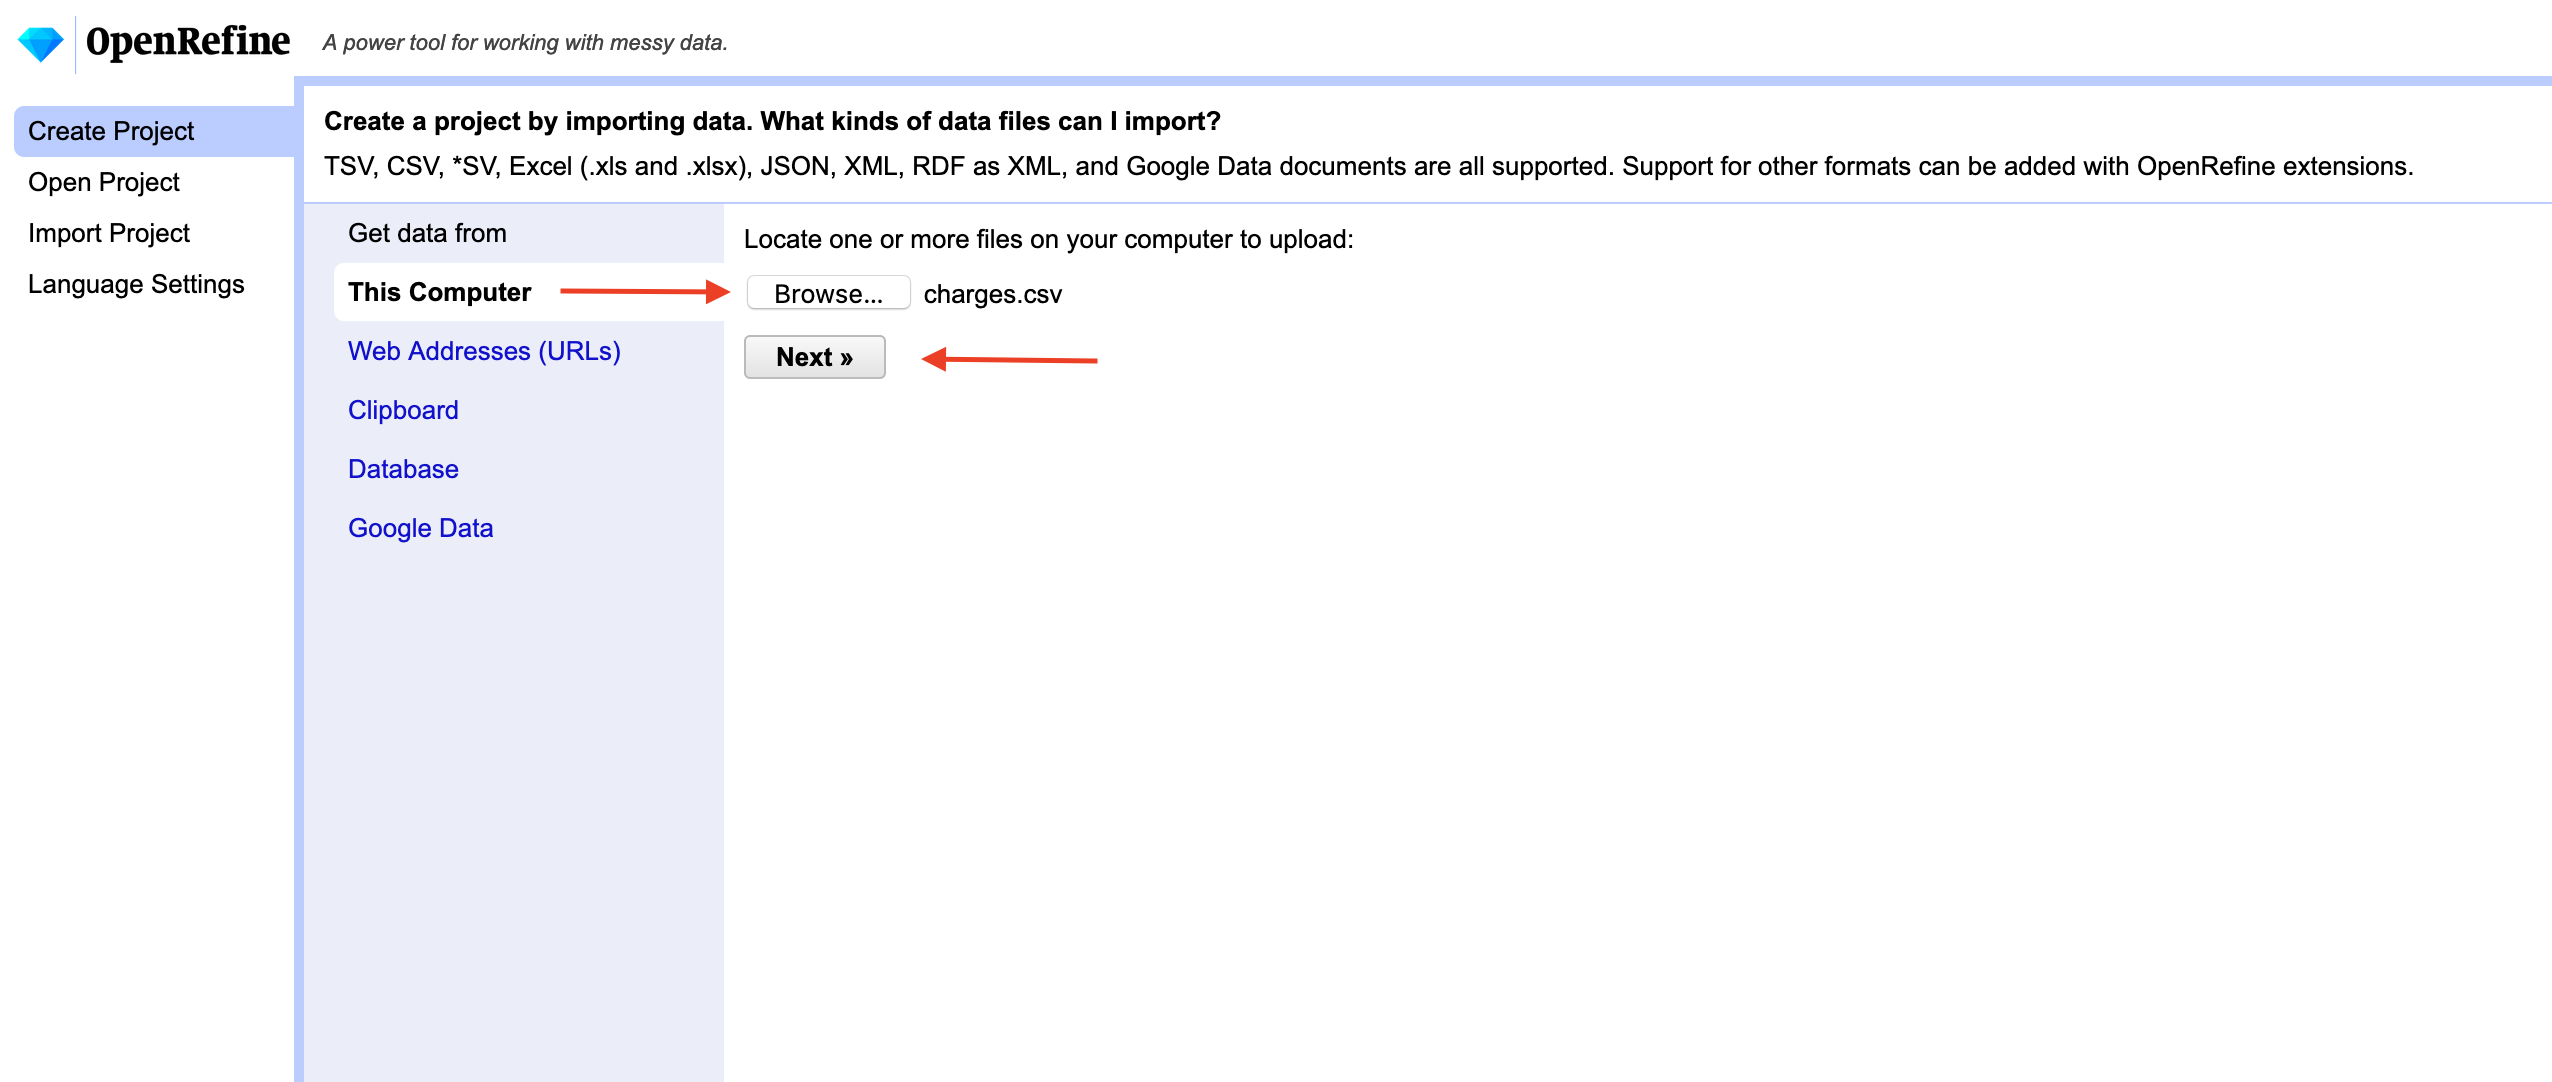
\includegraphics[width=35.44in]{images/open1}

After your data is loaded into the app, you'll get a screen to look over what the data looks like. On the top right corner, you'll see a button to create the project.

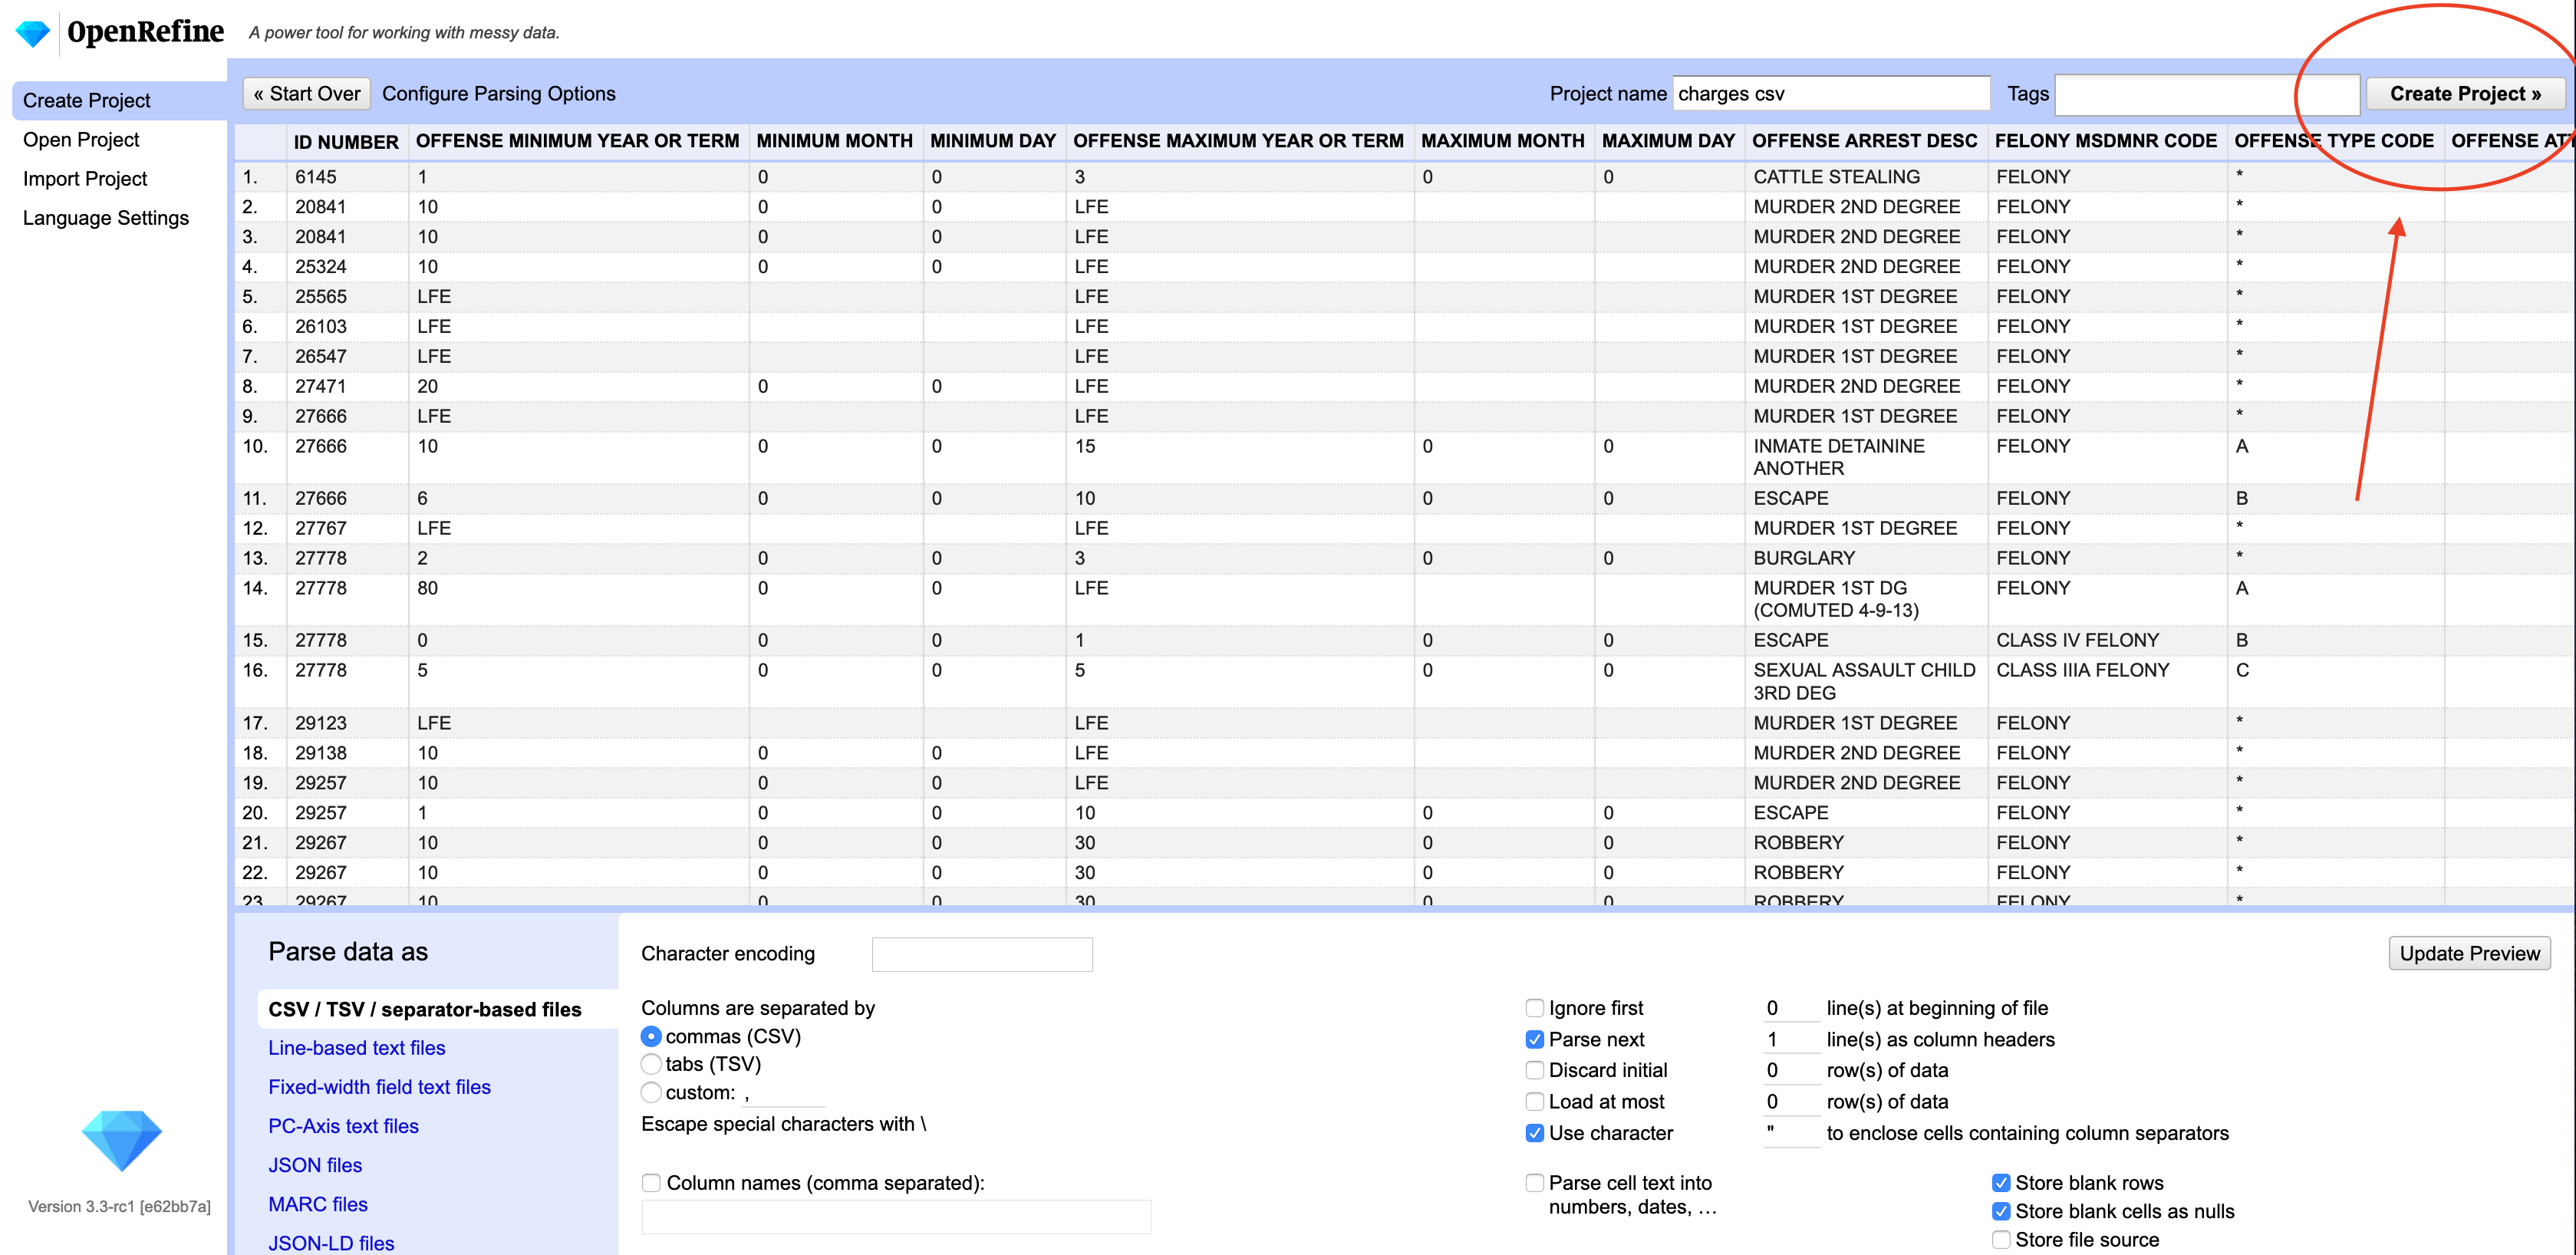
\includegraphics[width=46.64in]{images/open2}

The real power in Open Refine is in faceting. In our case, we're specifically going to use text faceting. Next to the OFFENSE ARREST DESC header, click the down arrow, then facet, then text facet.

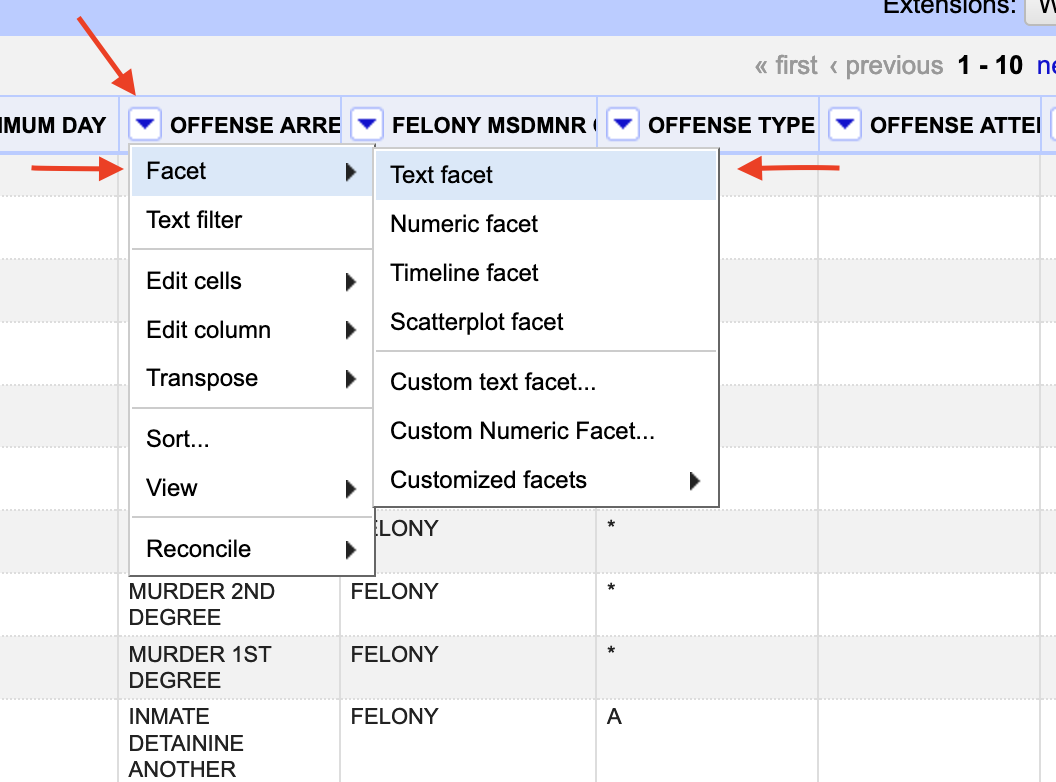
\includegraphics[width=14.67in]{images/open3}

After that, a new box will appear on the left. It tells us how many unique offenses are there: 4,082. And, there's a button on the right of the box that says Cluster. Click that.

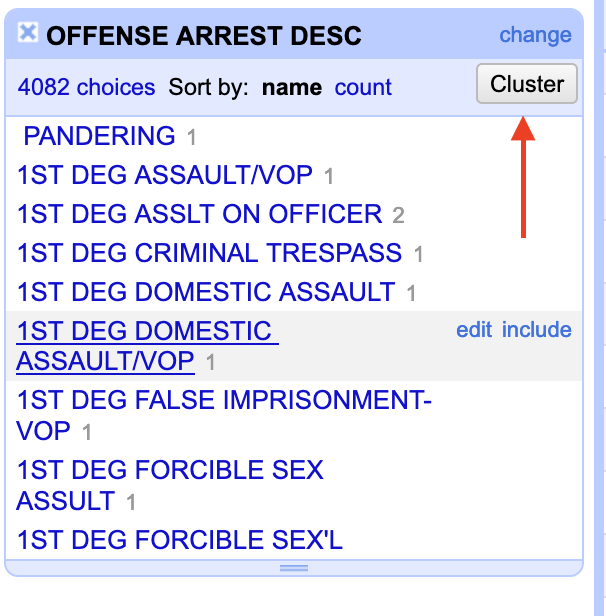
\includegraphics[width=8.42in]{images/open4}

The default clustering algorithm used is key collision, using the fingerprint function. This is the same method we used with Sheridan County above.

At the top, you'll see which method was used, and how many clusters that algorithm identified. Then, below that, you can see what those clusters are. Then, using human judgement, you can say if you agree with the cluster. If you do, click the merge checkbox. When it merges, the new result will be what it says in New Cell Value. Most often, that's the row with the most common result.

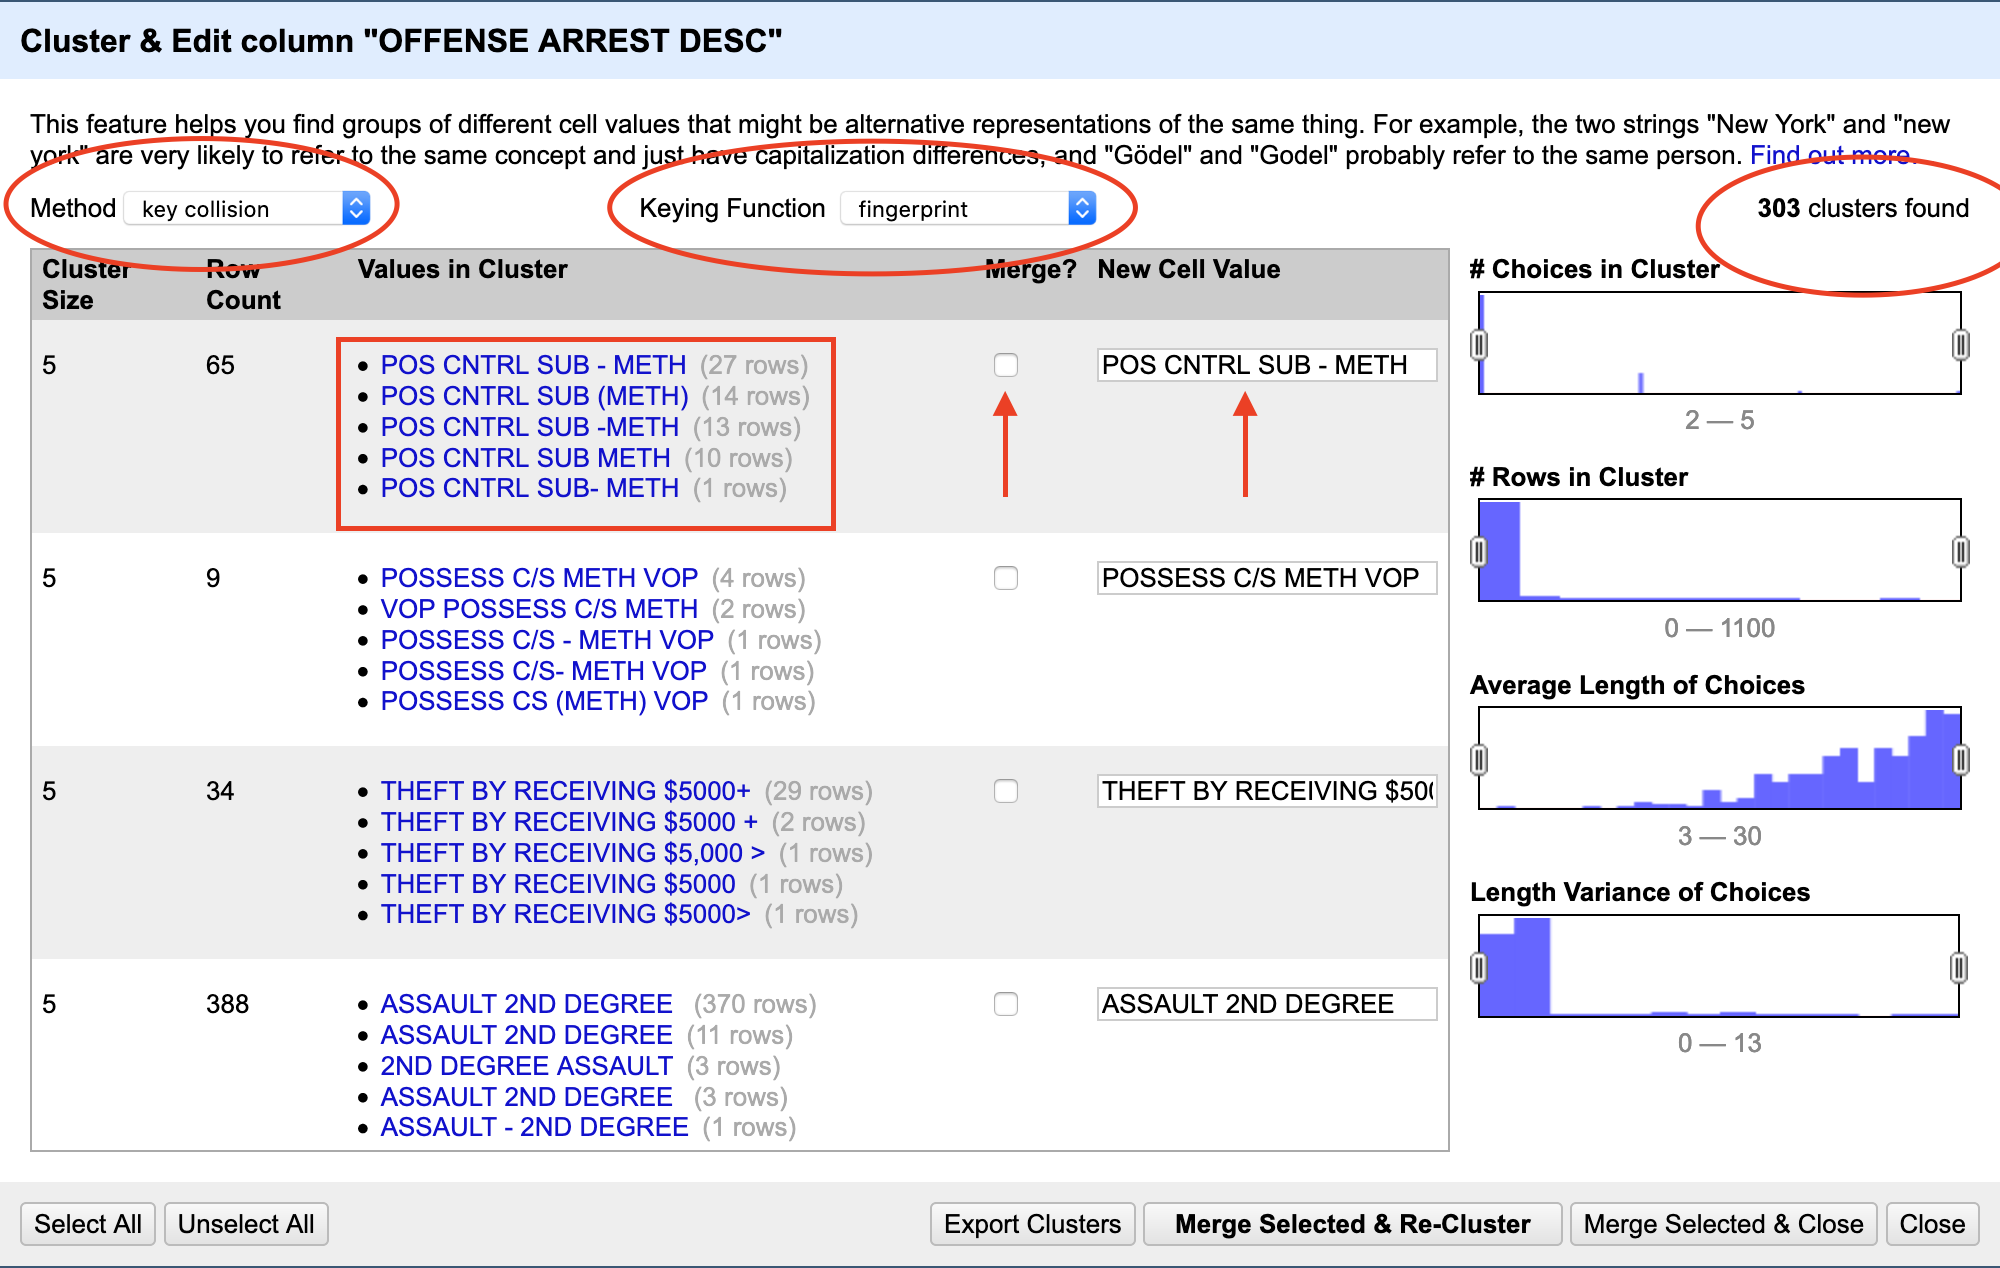
\includegraphics[width=27.78in]{images/open6}

Now begins the fun part: You have to look at all 303 clusters found and decide if they are indeed valid. The key collision method is very good, and very conservative. You'll find that most of them are usually valid.

When you're done, click Merge Selected and Re-Cluster.

If any new clusters come up, evaluate them. Repeat until either no clusters come up or the clusters that do come up are ones you reject.

Now. Try a new method. Rinse and repeat. You'll keep doing this, and if the dataset is reasonably clean, you'll find the end.

If it's not, it'll go on forever.

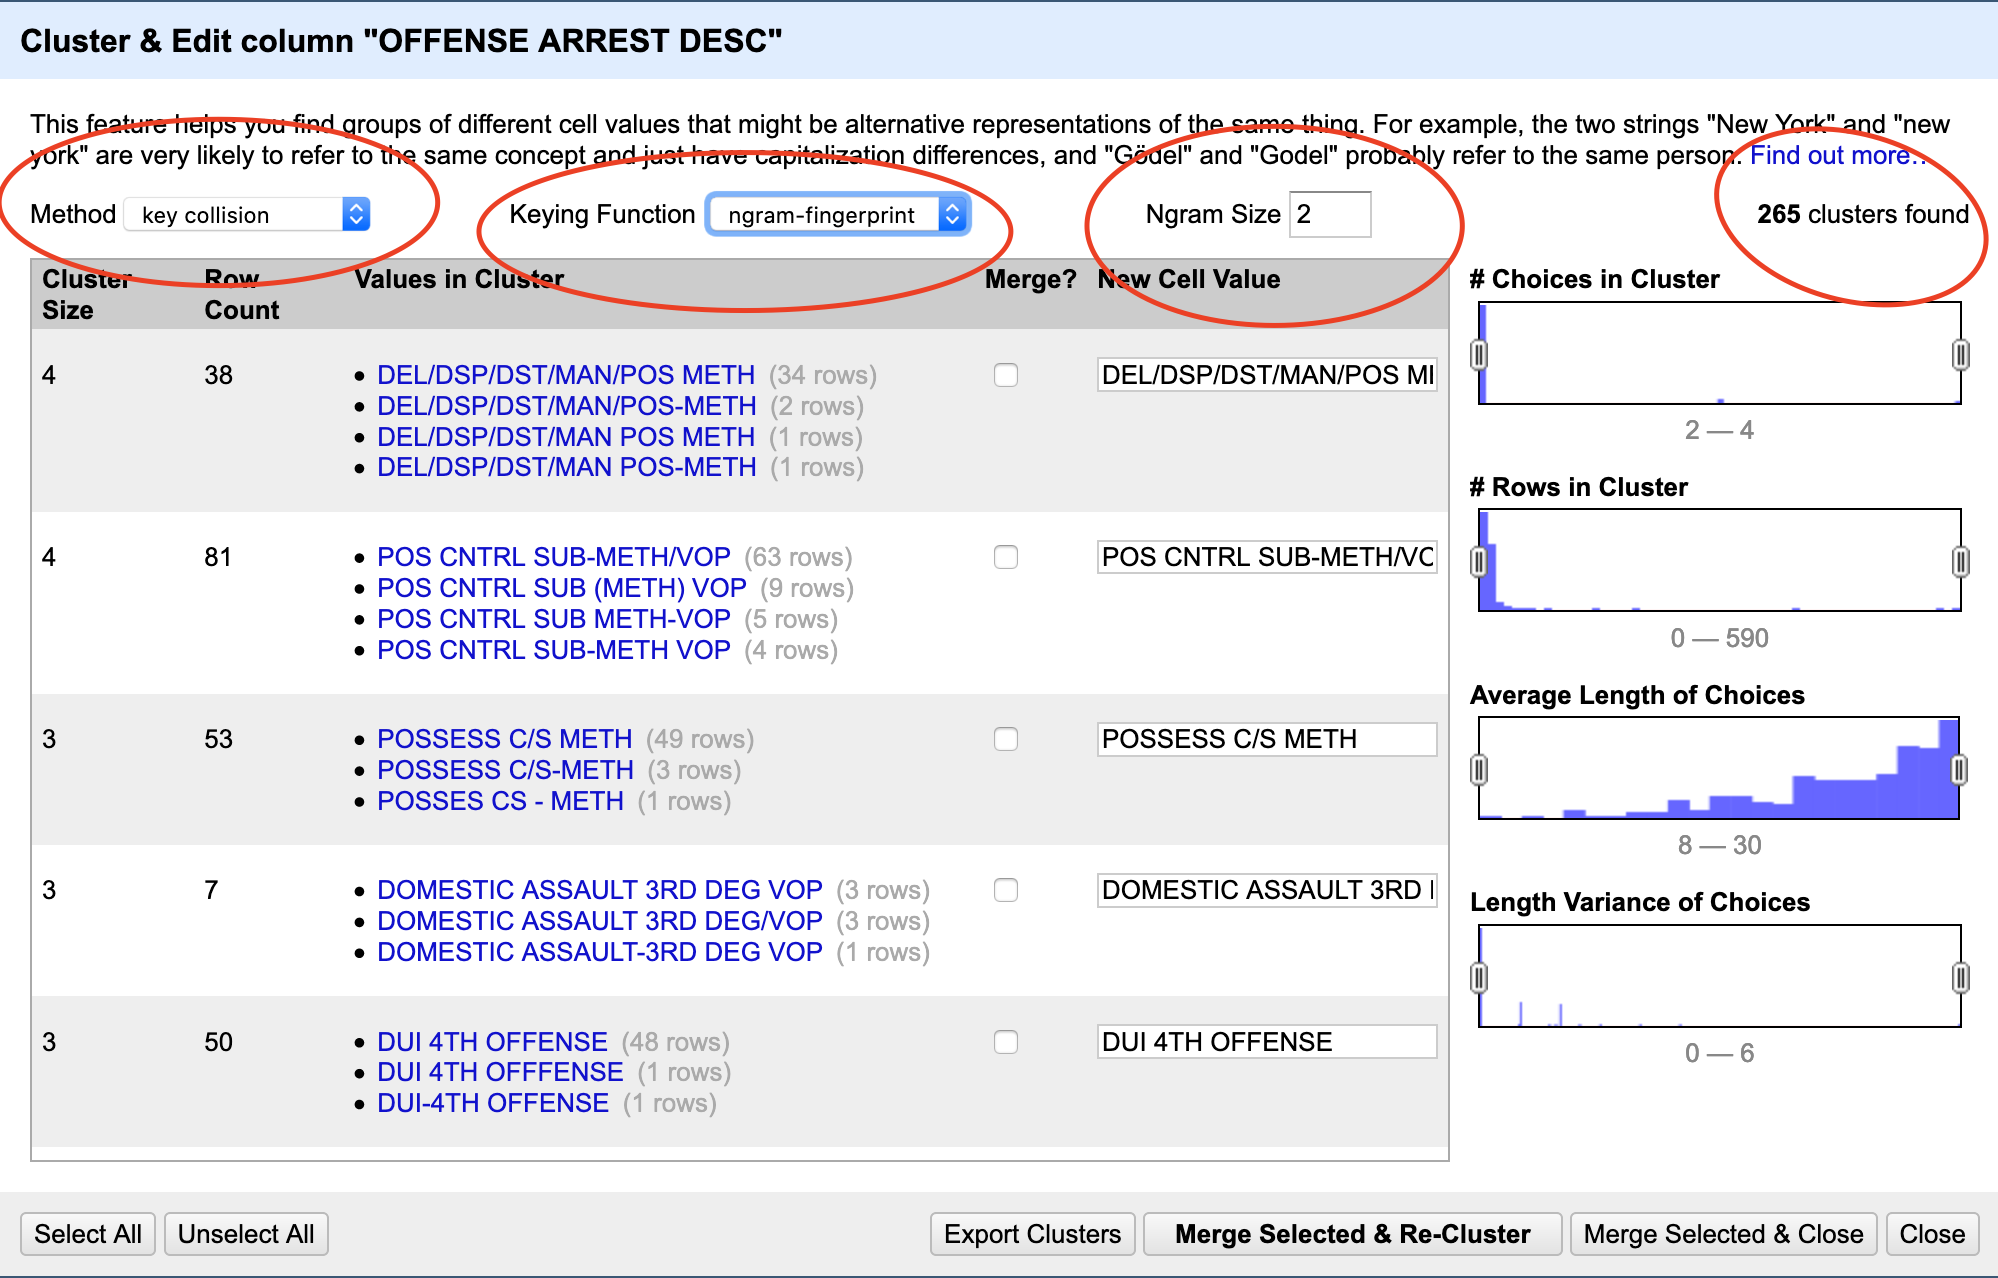
\includegraphics[width=27.75in]{images/open7}

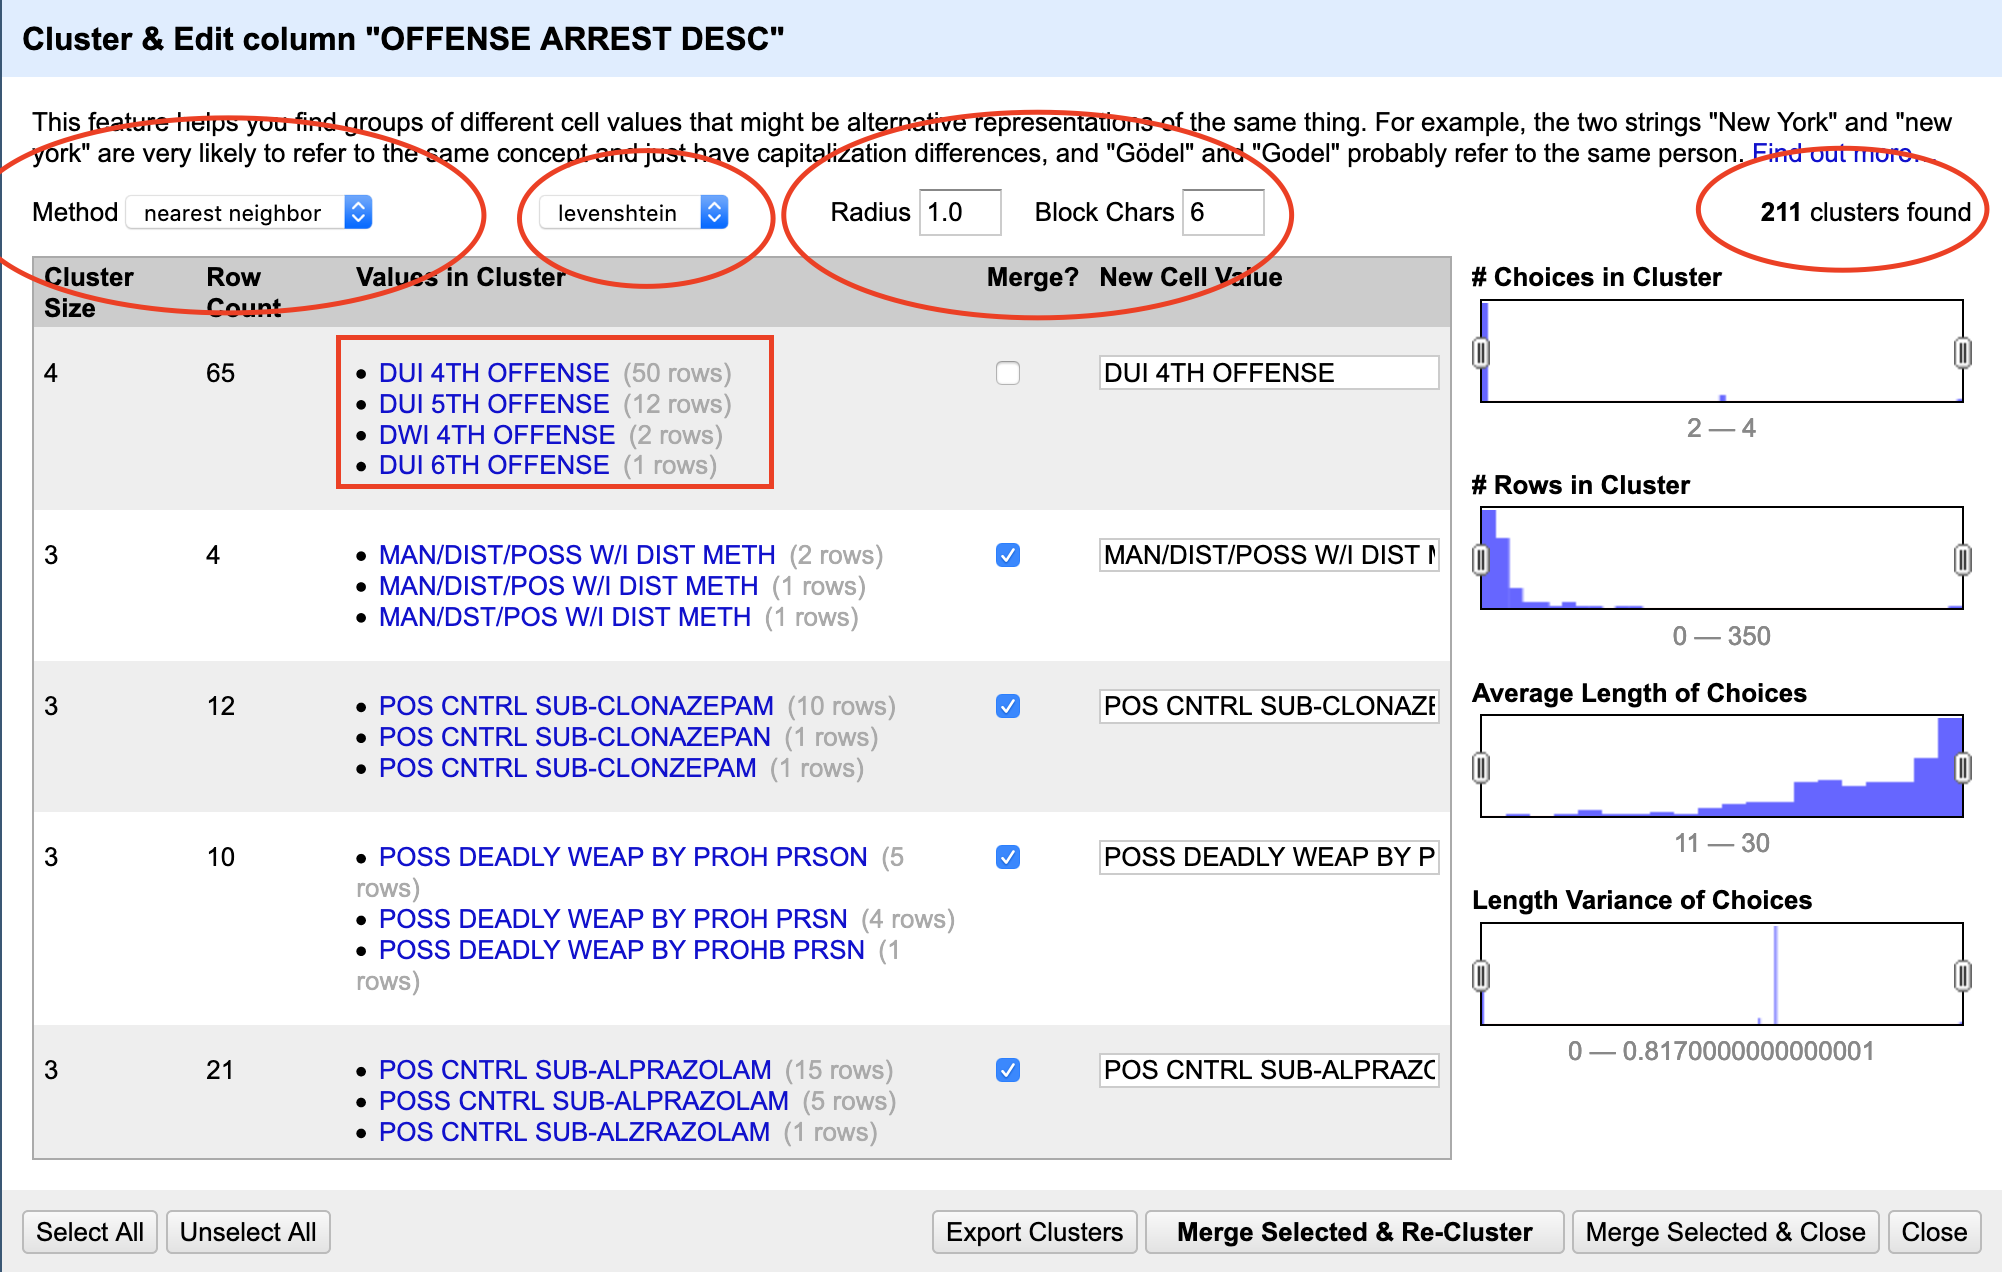
\includegraphics[width=27.81in]{images/open8}

A question for all data analysts -- if the dataset is bad enough, can it ever be cleaned?

There's no good answer. You have to find it yourself.

\hypertarget{cleaning-data-part-iv-pdfs}{%
\chapter{Cleaning Data Part IV: PDFs}\label{cleaning-data-part-iv-pdfs}}

The next circle of Hell on the Dante's Inferno of Data Journalism is the PDF. Governments everywhere love the PDF and publish all kinds of records in a PDF. The problem is a PDF isn't a data format -- it's a middle finger, saying I've Got Your Accountability Right Here, Pal.

It's so ridiculous that there's a constellation of tools that do nothing more than try to harvest tables out of PDFs. There are online services like \href{https://www.cometdocs.com/}{CometDocs} where you can upload your PDF and point and click your way into an Excel file. There are mobile device apps that take a picture of a table and convert it into a spreadsheet. But one of the best is a tool called \href{https://tabula.technology/}{Tabula}. It was build by journalists for journalists.

There is a version of Tabula that will run inside of R -- a library called Tabulizer -- but the truth is I'm having the hardest time installing it on my machine, which leads me to believe that trying to install it across a classroom of various machines would be disasterous. The standalone version works just fine.

Unfortunately, harvesting tables from PDFs with Tabula is an exercise in getting your hopes up, only to have them dashed. We'll start with an example.

\hypertarget{when-it-looks-good-but-goes-wrong}{%
\section{When it looks good, but goes wrong}\label{when-it-looks-good-but-goes-wrong}}

Every year, the University of Nebraska-Lincoln publishes dozens of PDFs that give you interesting demographic information about students, the faculty and a variety of other things. But all of it -- every little bit of it -- is in a PDF. And most of them are designed to look ``nice'' not convey data. Even when they do very obviously look like they came from a spreadsheet -- like someone printed the spreadsheet to a PDF so they could put it on the web -- it doesn't work.

A perfect example of this is the data showing the \href{https://iea.unl.edu/dmdocuments/050_fall_2018_enrl_p100.pdf}{breakdown of students by degree, major, race and sex}. Open it up, it looks like a spreadsheet but in a PDF.

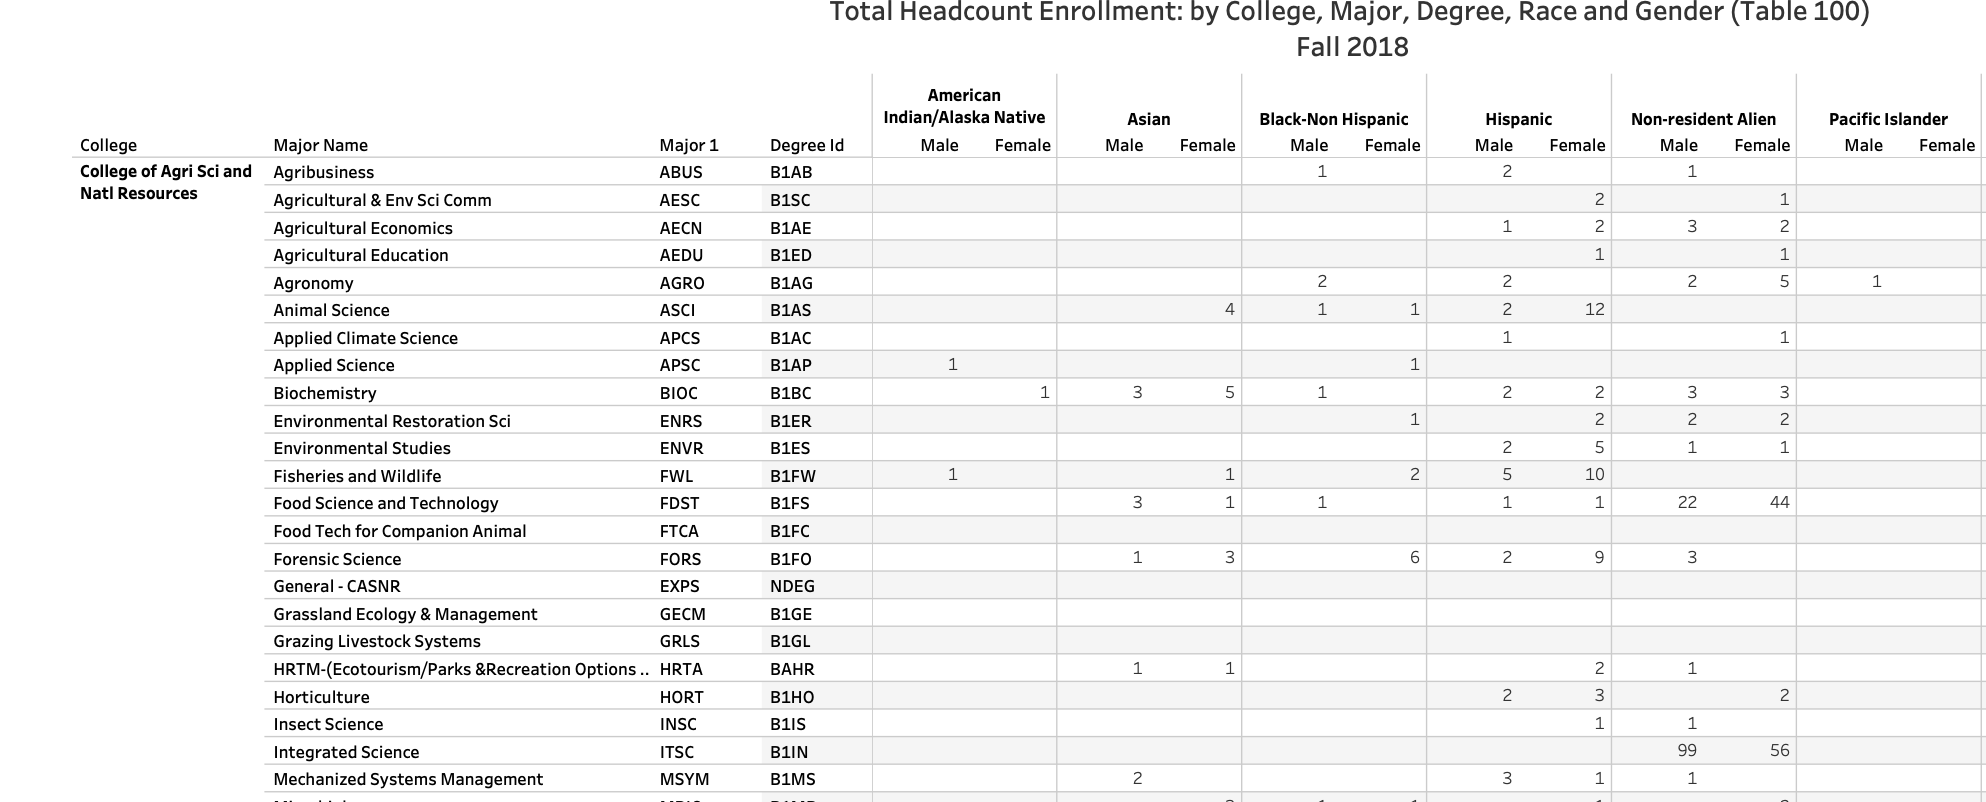
\includegraphics[width=27.58in]{images/pdfs1}

\href{https://tabula.technology/}{Download and install Tabula}. Tabula works much the same way as Open Refine does -- it works in the browser by spinning up a small webserver in
your computer.

When Tabula opens, you click browse to find the PDF on your computer somewhere, and then click import.

After it imports, click autodetect tables. You'll see red boxes appear around what Tabula believes are the tables. You'll see it does a pretty good job at this.

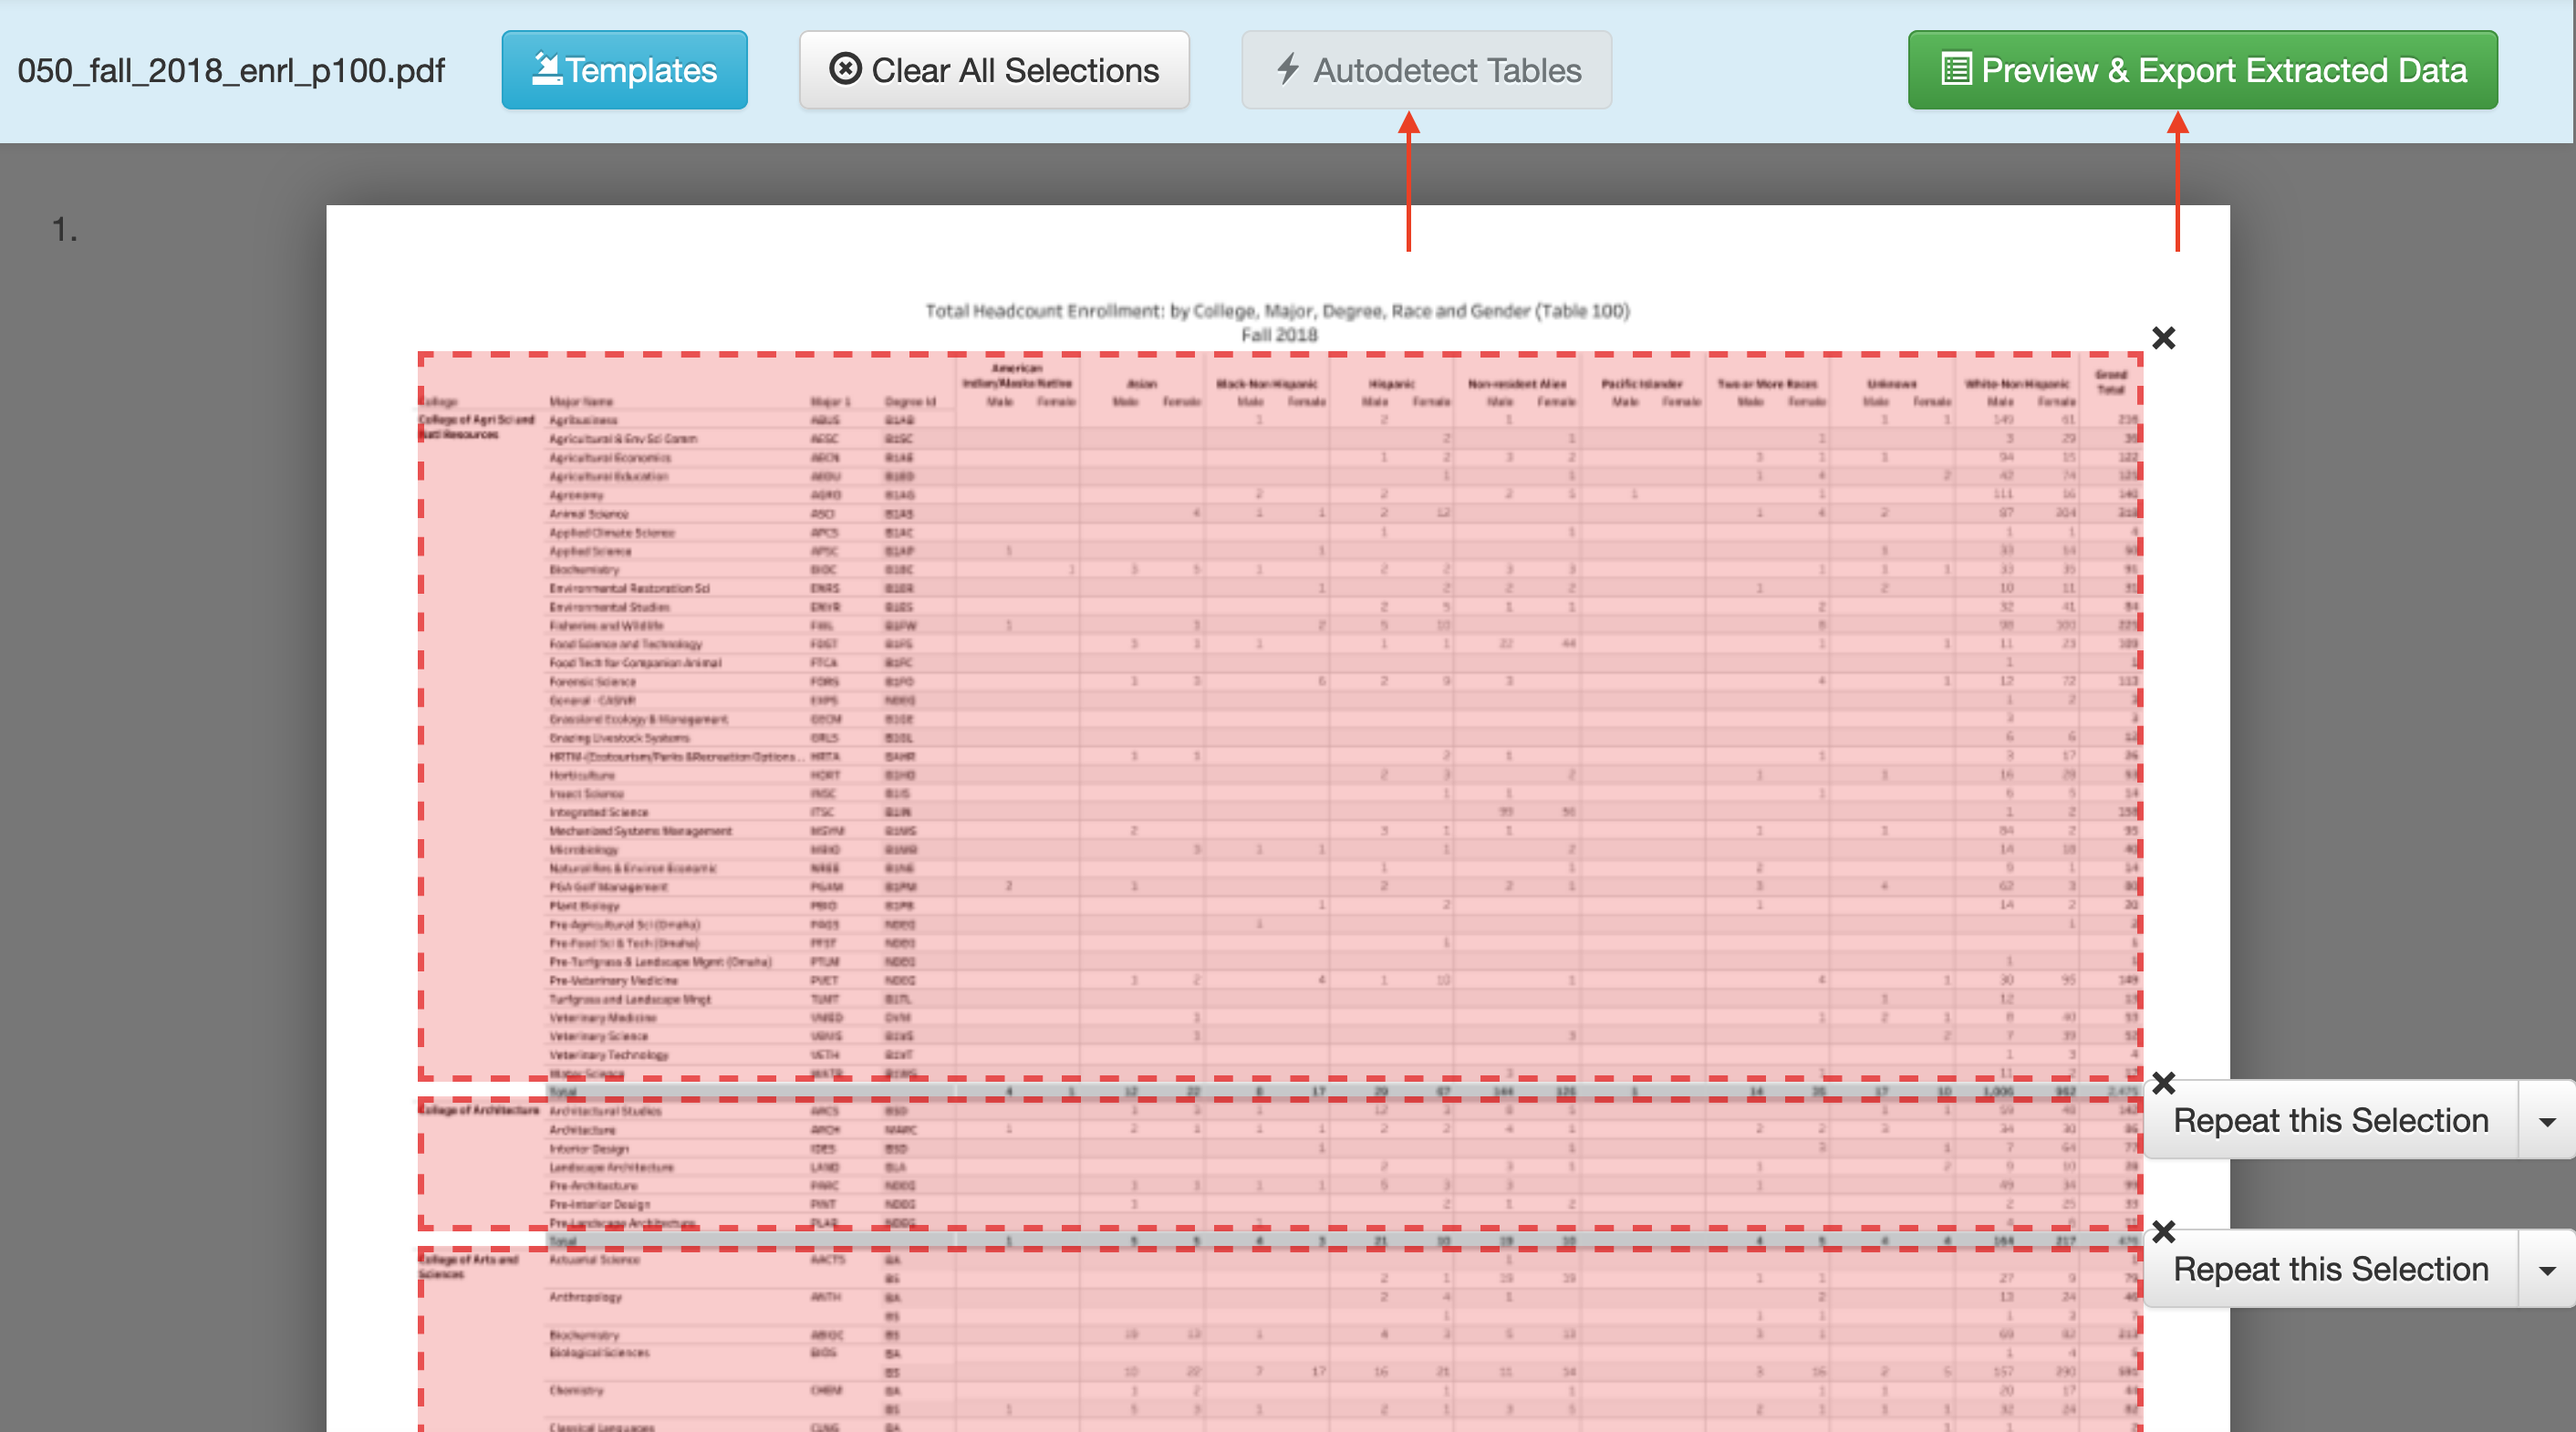
\includegraphics[width=39.22in]{images/pdfs2}

If you like what you see, click Preview and Export Extracted Data.

And here's where it all starts to go wrong.

You'll see at first it looks good -- you get a reasonable representation of the table. But look at the first line.

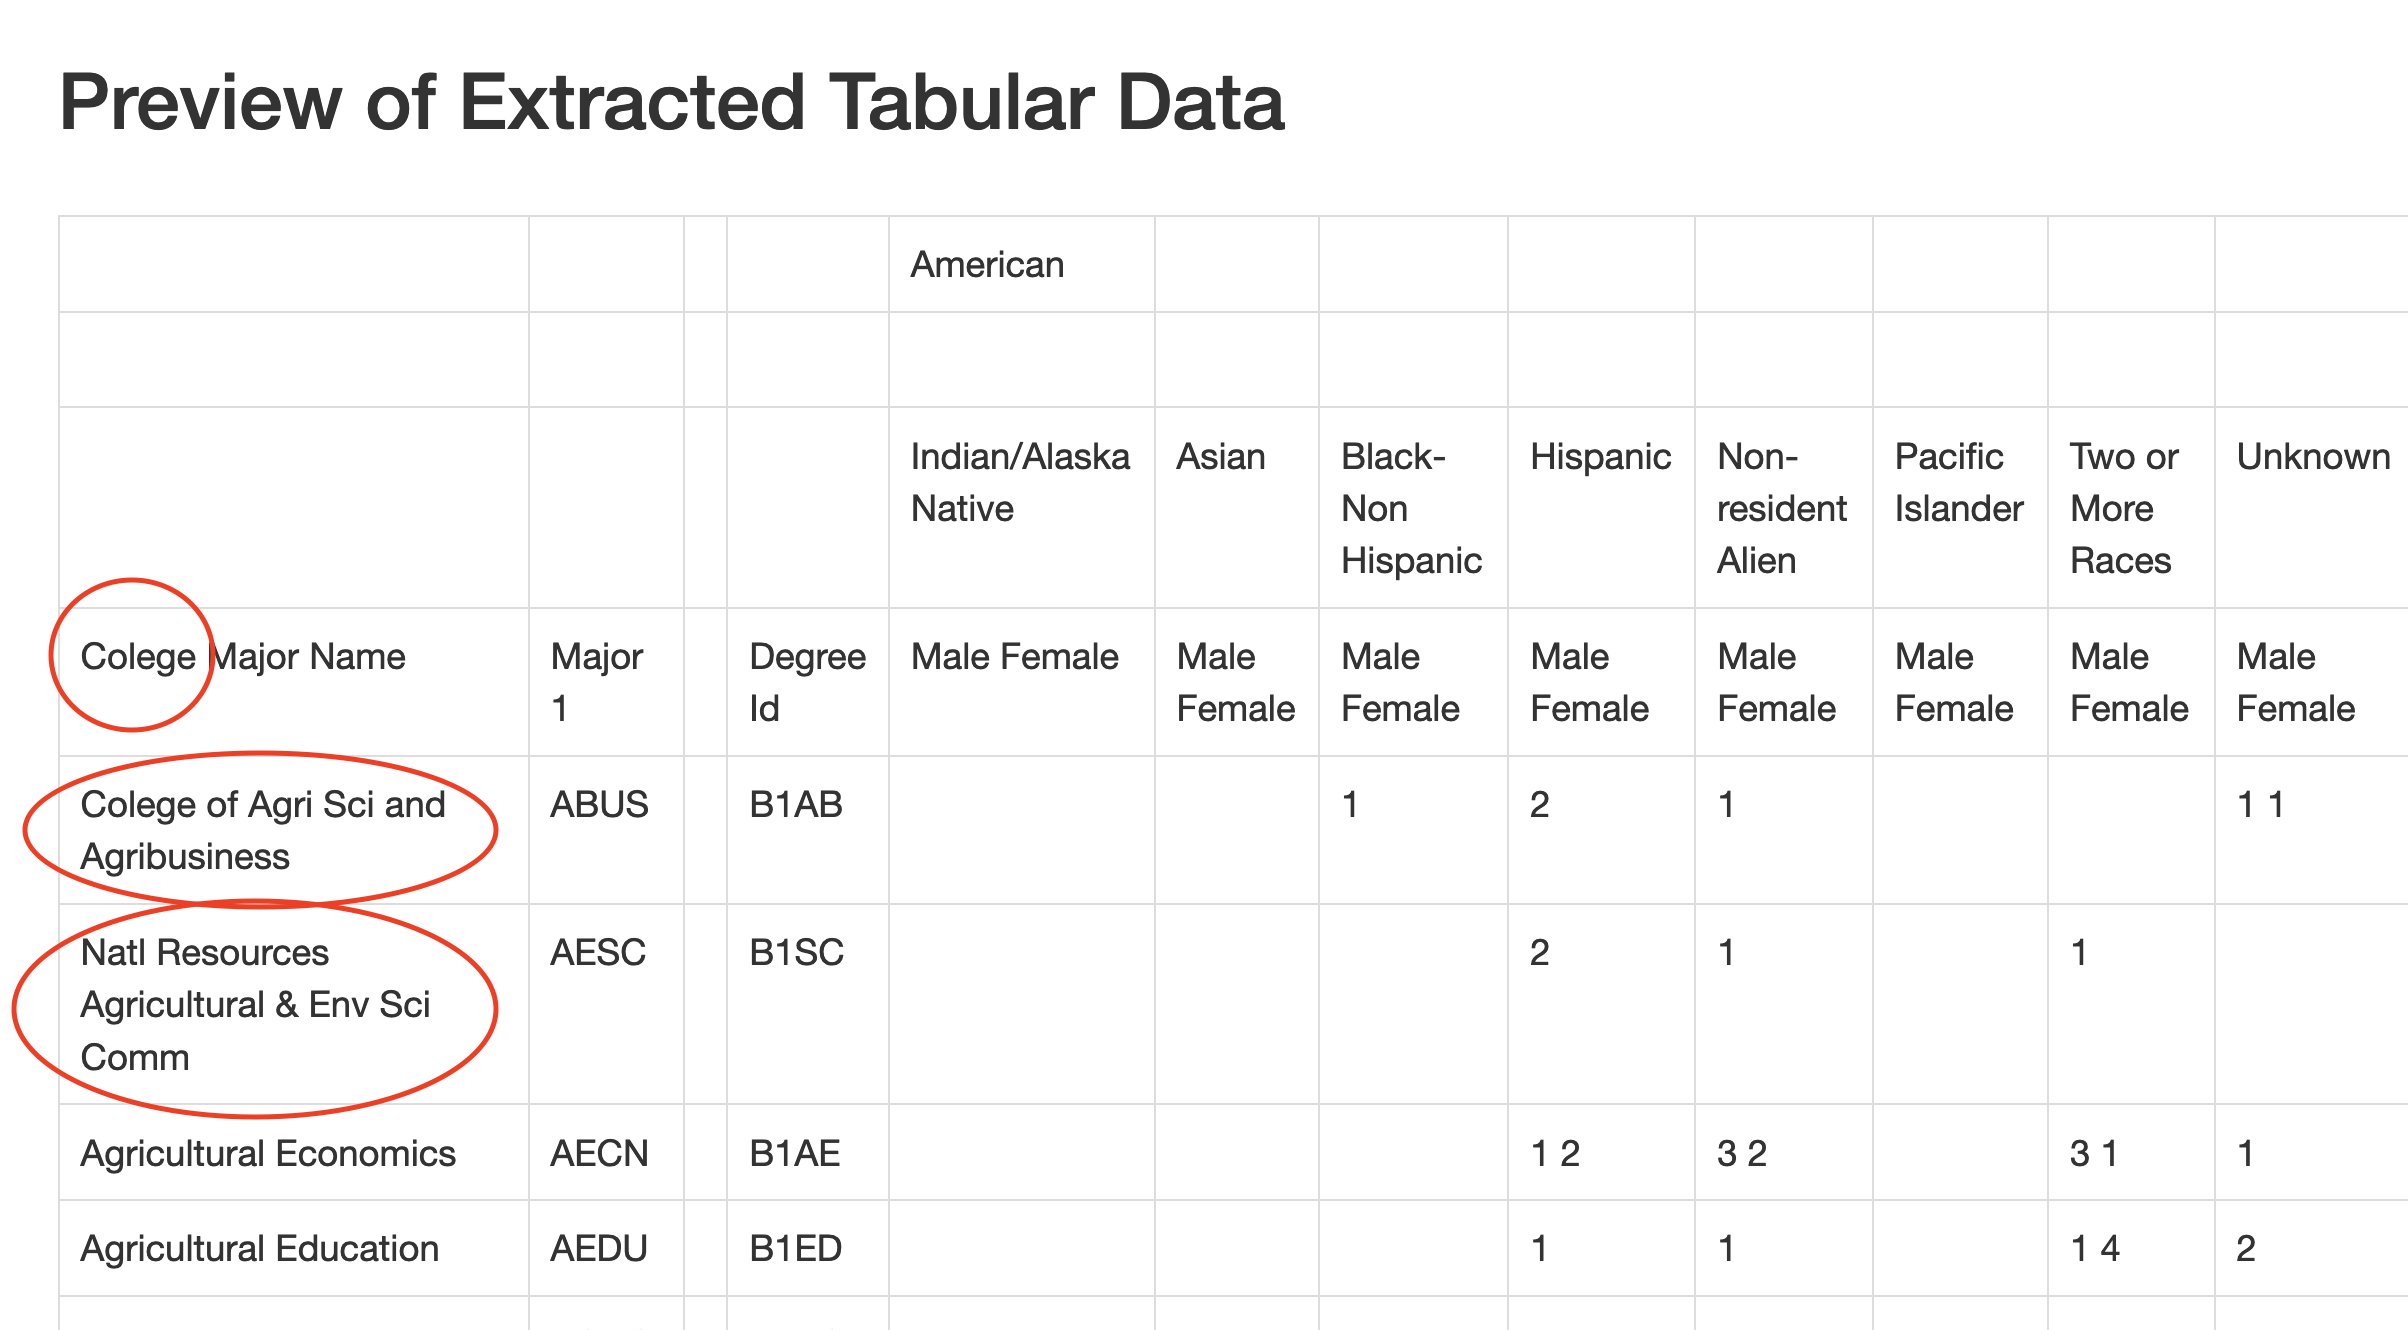
\includegraphics[width=33.44in]{images/pdfs3}

First, the misspelling of college is disturbing. Did a university document misspell it? No.~Which means Tabula is reading two ls as one. That's \ldots{} not good.

Second, notice how the College of Agri Sci and Natl Resources, which was in it's own column before have been merged, somewhat inartfully, into the first column of major names. There is no major Colege of Agri Sci and Agribusiness. Same with Natl Resources Agricultural \& Env Sci Comm. Those aren't things.

Note the empty column between Major1 and DegreeId.

Now scroll down some more.

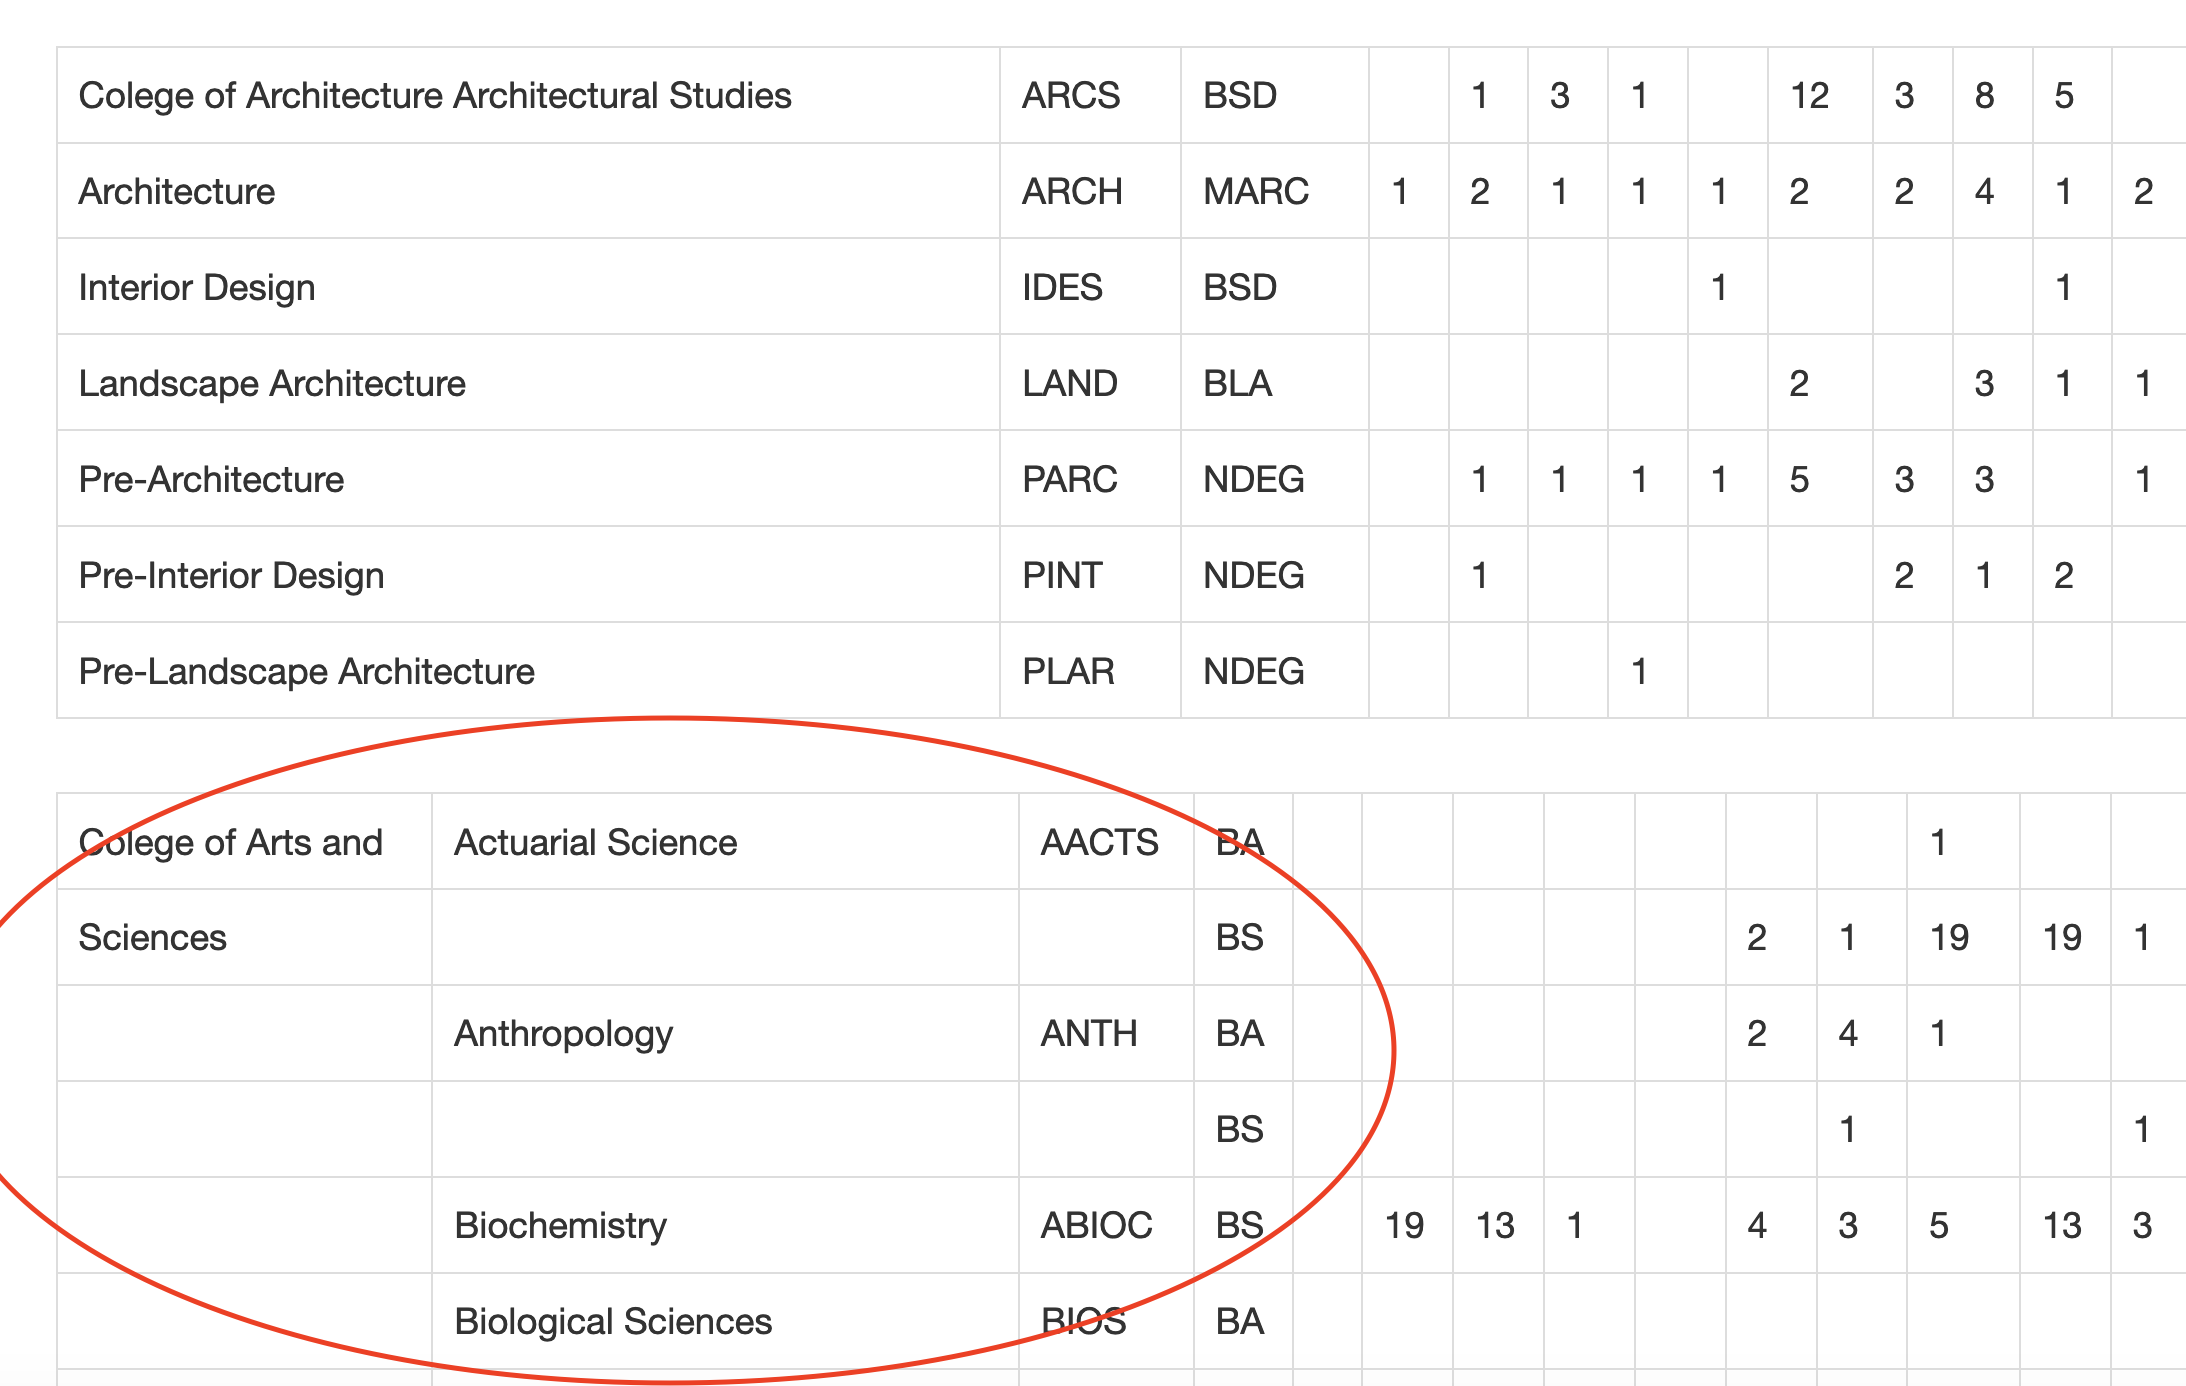
\includegraphics[width=30.36in]{images/pdfs4}

Notice Architecture has the same merging of college name and first major problems as the first one does, but note the blank column is missing.

Look at Arts and Sciences. Arts and Sciences are now in their own column, as the data shows, but there's now empty names that shouldn't be. What are those?

In short, it's a mess.

Here's the sad truth: THIS IS PRETTY GOOD. Open it in a spreadsheet and a little copying and pasting work while double checking the right names line up with the right rows and you're in business. As converted PDFs, this isn't bad.

It beats typing it out.

\hypertarget{when-it-works-well.}{%
\section{When it works well.}\label{when-it-works-well.}}

Each month, the Nebraska Department of Revenue releases the monthly tax receipts of the state, and forecasts into the future what tax receipts might be in the near future. They do this for planning purposes -- the Legislature needs to know how much money the state may have when the new budget is put into place so they know how much money they have to spend.

\href{https://revenue.nebraska.gov/about/news-releases/previous-general-funds-receipts-news-releases}{The announcement comes in a press release}. Each press release includes a table showing the current number, the predicted number, and difference. Of course it's a PDF.

Let's look at the most recent month as of this writing: \href{https://revenue.nebraska.gov/sites/revenue.nebraska.gov/files/doc/news-release/gen-fund/2020/General_Fund_Receipts_January_2020.pdf}{January 2020}. Download it, open it in Tabula and hit Autodetect tables.

You'll note it finds no tables on the first page. Which is good, because there aren't any. Let's look at the third page. It finds a table, but is it one?

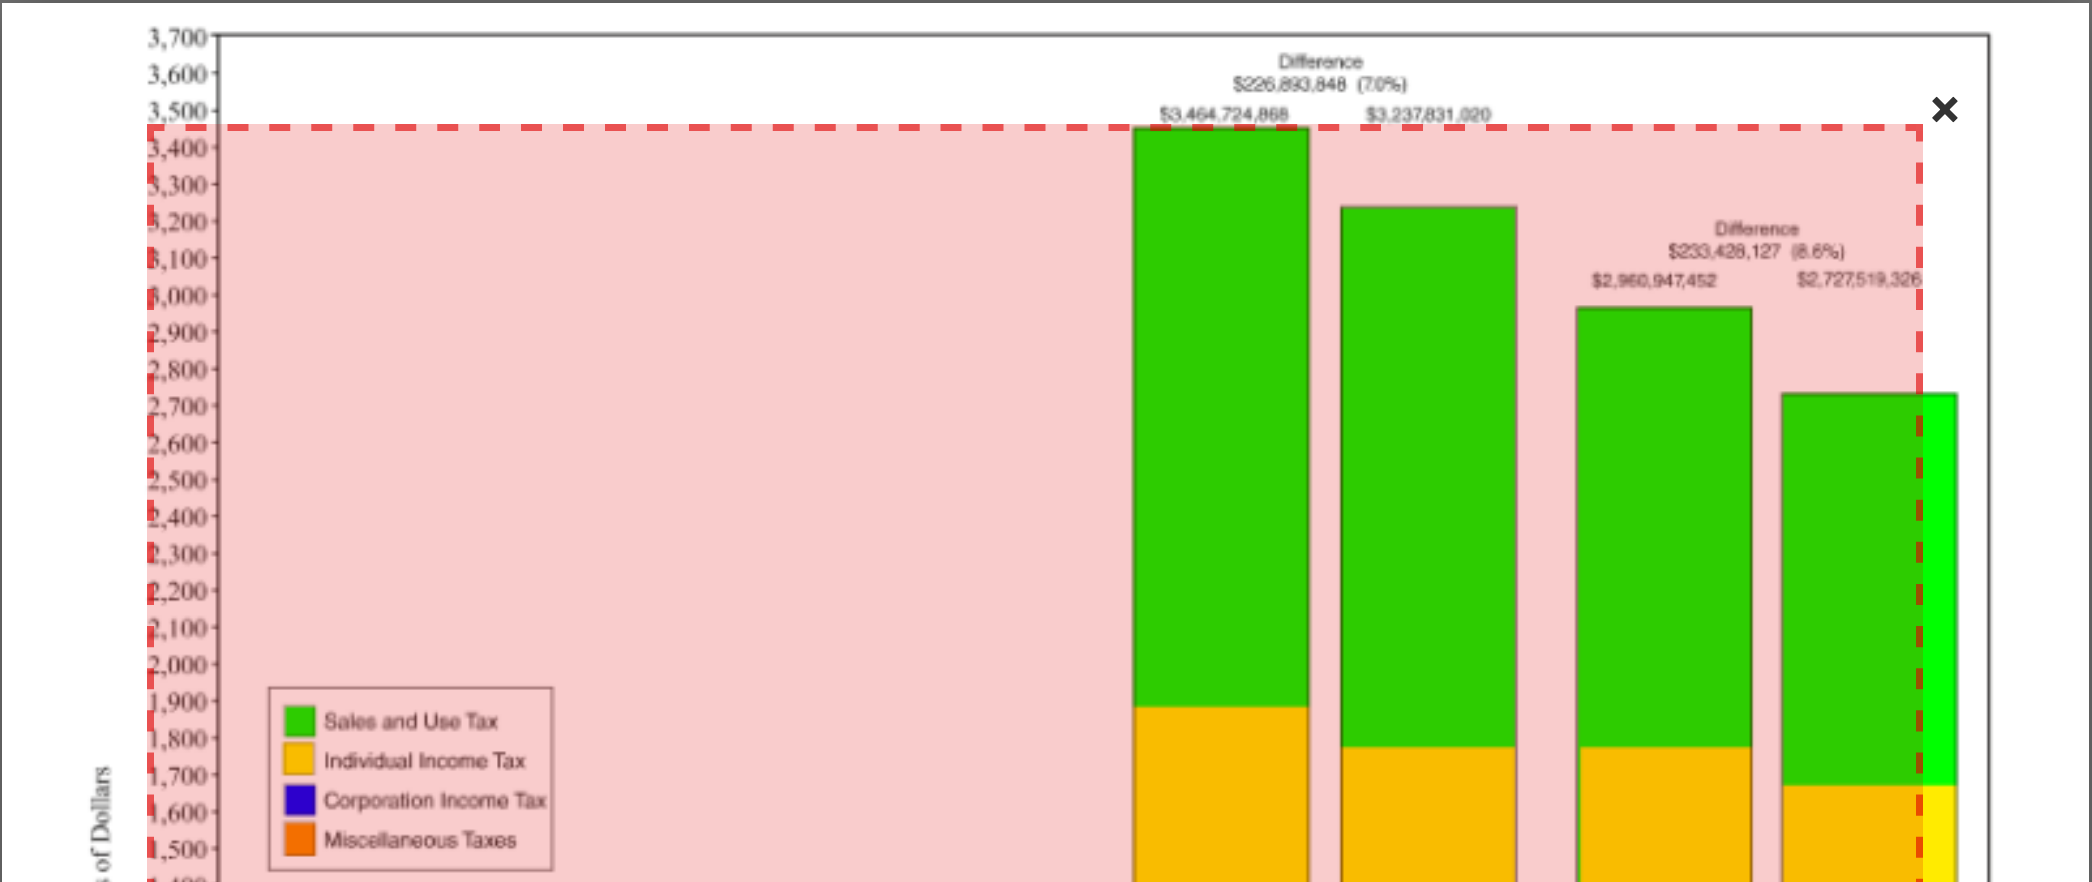
\includegraphics[width=29.06in]{images/pdfs5}

Let's hit the X in the top right on that one.

That leaves page 2. It finds two tables there. Let's just grab the first. Hit X on the second and click to preview the extracted data.

This looks good. So let's export it to a csv.

\hypertarget{cleaning-up-the-data-in-r}{%
\section{Cleaning up the data in R}\label{cleaning-up-the-data-in-r}}

The good news is that we have data we don't have to retype. The bad news is, it's hardly in importable shape.

Let's load libraries.

\begin{Shaded}
\begin{Highlighting}[]
\KeywordTok{library}\NormalTok{(tidyverse)}
\end{Highlighting}
\end{Shaded}

To import this, we need one row of headers. We have three. And we need headers that make sense.

We can spell these out in the import step. First, we'll use \texttt{skip} to skip the first three lines. Then we'll spell out the column names by hand in a \texttt{col\_names} bit. Here's how it looks.

\begin{Shaded}
\begin{Highlighting}[]
\NormalTok{receipts <-}\StringTok{ }\KeywordTok{read_csv}\NormalTok{(}\StringTok{"data/tabula-General_Fund_Receipts_January_2020.csv"}\NormalTok{, }\DataTypeTok{skip =} \DecValTok{3}\NormalTok{, }\DataTypeTok{col_names =} \KeywordTok{c}\NormalTok{(}\StringTok{"Month"}\NormalTok{, }\StringTok{"TotalActualNetReceipts"}\NormalTok{, }\StringTok{"TotalProjectedNetReceipts"}\NormalTok{, }\StringTok{"Difference"}\NormalTok{, }\StringTok{"PercentDifference"}\NormalTok{, }\StringTok{"CumulativeActualNetReceipts"}\NormalTok{, }\StringTok{"CumulativeProjectedNetReceipts"}\NormalTok{, }\StringTok{"CumulativeDifference"}\NormalTok{,}\StringTok{"CumulativePercentDifference"}\NormalTok{), }\DataTypeTok{skip_empty_rows =} \OtherTok{TRUE}\NormalTok{)}
\end{Highlighting}
\end{Shaded}

\begin{verbatim}
## Parsed with column specification:
## cols(
##   Month = col_character(),
##   TotalActualNetReceipts = col_character(),
##   TotalProjectedNetReceipts = col_character(),
##   Difference = col_character(),
##   PercentDifference = col_character(),
##   CumulativeActualNetReceipts = col_character(),
##   CumulativeProjectedNetReceipts = col_character(),
##   CumulativeDifference = col_character(),
##   CumulativePercentDifference = col_character()
## )
\end{verbatim}

Now we have a harder part.

The columns come in as character columns. Why? Because the state puts commas and \$ and \% in them, which R does not interpret as anything except text. So we need to get rid of them. We can mutate columns and use a function called \texttt{gsub} that finds a string and replaces it with something. So in our case, we're going to \texttt{gsub(",","",\ fieldname)}. The unfortunate part is we have a lot of colunns and a lot of fixes. So this is going to require a lot of code. It is repetitive, though, so we can copy and paste and adjust with most of it.

At the end, we need to use a function called \texttt{mutate\_at} and convert the columns that aren't text into numbers.

And one last thing: If we do many months of this, we should note which report this comes from. We can do this with mutate as well.

Here's what that looks like:

\begin{Shaded}
\begin{Highlighting}[]
\NormalTok{receipts }\OperatorTok\StringTok{ }\KeywordTok{mutate}\NormalTok{(}
  \DataTypeTok{TotalActualNetReceipts =} \KeywordTok{gsub}\NormalTok{(}\StringTok{","}\NormalTok{,}\StringTok{""}\NormalTok{,TotalActualNetReceipts),}
  \DataTypeTok{TotalActualNetReceipts =} \KeywordTok{gsub}\NormalTok{(}\StringTok{"}\CharTok{\textbackslash{}\textbackslash{}}\StringTok{$"}\NormalTok{,}\StringTok{""}\NormalTok{,TotalActualNetReceipts),}
  \DataTypeTok{TotalProjectedNetReceipts =} \KeywordTok{gsub}\NormalTok{(}\StringTok{","}\NormalTok{,}\StringTok{""}\NormalTok{,TotalProjectedNetReceipts),}
  \DataTypeTok{TotalProjectedNetReceipts =} \KeywordTok{gsub}\NormalTok{(}\StringTok{"}\CharTok{\textbackslash{}\textbackslash{}}\StringTok{$"}\NormalTok{,}\StringTok{""}\NormalTok{,TotalProjectedNetReceipts),}
  \DataTypeTok{Difference =} \KeywordTok{gsub}\NormalTok{(}\StringTok{","}\NormalTok{,}\StringTok{""}\NormalTok{,Difference),}
  \DataTypeTok{Difference =} \KeywordTok{gsub}\NormalTok{(}\StringTok{"}\CharTok{\textbackslash{}\textbackslash{}}\StringTok{$"}\NormalTok{,}\StringTok{""}\NormalTok{,Difference),}
  \DataTypeTok{PercentDifference =} \KeywordTok{gsub}\NormalTok{(}\StringTok{"}\CharTok{\textbackslash{}\textbackslash{}}\StringTok{%"}\NormalTok{,}\StringTok{""}\NormalTok{,PercentDifference),}
  \DataTypeTok{CumulativeActualNetReceipts =} \KeywordTok{gsub}\NormalTok{(}\StringTok{","}\NormalTok{,}\StringTok{""}\NormalTok{,CumulativeActualNetReceipts),}
  \DataTypeTok{CumulativeActualNetReceipts =} \KeywordTok{gsub}\NormalTok{(}\StringTok{"}\CharTok{\textbackslash{}\textbackslash{}}\StringTok{$"}\NormalTok{,}\StringTok{""}\NormalTok{,CumulativeActualNetReceipts),}
  \DataTypeTok{CumulativeProjectedNetReceipts =} \KeywordTok{gsub}\NormalTok{(}\StringTok{","}\NormalTok{,}\StringTok{""}\NormalTok{,CumulativeProjectedNetReceipts),}
  \DataTypeTok{CumulativeProjectedNetReceipts =} \KeywordTok{gsub}\NormalTok{(}\StringTok{"}\CharTok{\textbackslash{}\textbackslash{}}\StringTok{$"}\NormalTok{,}\StringTok{""}\NormalTok{,CumulativeProjectedNetReceipts),}
  \DataTypeTok{CumulativeDifference =} \KeywordTok{gsub}\NormalTok{(}\StringTok{","}\NormalTok{,}\StringTok{""}\NormalTok{,CumulativeDifference),}
  \DataTypeTok{CumulativeDifference =} \KeywordTok{gsub}\NormalTok{(}\StringTok{"}\CharTok{\textbackslash{}\textbackslash{}}\StringTok{$"}\NormalTok{,}\StringTok{""}\NormalTok{,CumulativeDifference),}
  \DataTypeTok{CumulativePercentDifference =} \KeywordTok{gsub}\NormalTok{(}\StringTok{"}\CharTok{\textbackslash{}\textbackslash{}}\StringTok{%"}\NormalTok{,}\StringTok{""}\NormalTok{,CumulativePercentDifference)}
\NormalTok{  ) }\OperatorTok\StringTok{ }\KeywordTok{mutate_at}\NormalTok{(}\KeywordTok{vars}\NormalTok{(}\OperatorTok{-}\NormalTok{Month), as.numeric) }\OperatorTok\StringTok{ }\KeywordTok{mutate}\NormalTok{(}\DataTypeTok{ReportMonth =} \StringTok{"January 2020"}\NormalTok{)}
\end{Highlighting}
\end{Shaded}

\begin{verbatim}
## # A tibble: 7 x 10
##   Month TotalActualNetR~ TotalProjectedN~ Difference PercentDifferen~
##   <chr>            <dbl>            <dbl>      <dbl>            <dbl>
## 1 July         284883132        271473079   13410054              4.9
## 2 Augu~        462019974        440504016   21515958              4.9
## 3 Sept~        551908013        510286143   41621870              8.2
## 4 Octo~        289723434        266204529   23518905              8.8
## 5 Nove~        431787603        404934524   26853079              6.6
## 6 Dece~        472926836        421455999   51470837             12.2
## 7 Janu~        467698460        412661036   55037424             13.3
## # ... with 5 more variables: CumulativeActualNetReceipts <dbl>,
## #   CumulativeProjectedNetReceipts <dbl>, CumulativeDifference <dbl>,
## #   CumulativePercentDifference <dbl>, ReportMonth <chr>
\end{verbatim}

We can now reuse this with other months after we harvest the data out of it.

\hypertarget{combining-and-joining}{%
\chapter{Combining and joining}\label{combining-and-joining}}

Often, as data journalists, we're looking at data across time or at data stored in multiple tables. And to do that, we need to often need to merge that data together.

Depending on what we have, we may just need to stack data on top of each other to make new data. If we have 2019 data and 2018 data and we want that to be one file, we stack them. If we have a dataset of cows in counties and a dataset of populations in county, we're going to join those two together on the county -- the common element.

Let's explore.

\hypertarget{combining-data}{%
\section{Combining data}\label{combining-data}}

In the last assignment, we harvested data out of PDFs. Let's reuse what we did there and merge three months of reports from the Department of Revenue together. For mine, I have \href{https://unl.box.com/s/nd1yaroltsy161pqgbges9xrtav2qdqp}{January 2020}, \href{https://unl.box.com/s/jfdtqffty1vb2zbil8z5qalu18yg0590}{December 2019}, and \href{https://unl.box.com/s/g1dc0mibxxutsitqssv2uf75pmb7avle}{November 2019}.

Let's do what we need to import them properly. Unlike the last example, I've merged it all into one step for each of the three datasets.

\begin{Shaded}
\begin{Highlighting}[]
\KeywordTok{library}\NormalTok{(tidyverse)}
\end{Highlighting}
\end{Shaded}

\begin{Shaded}
\begin{Highlighting}[]
\NormalTok{receiptsJan20 <-}\StringTok{ }\KeywordTok{read_csv}\NormalTok{(}\StringTok{"data/tabula-General_Fund_Receipts_January_2020.csv"}\NormalTok{, }\DataTypeTok{skip =} \DecValTok{3}\NormalTok{, }\DataTypeTok{col_names =} \KeywordTok{c}\NormalTok{(}\StringTok{"Month"}\NormalTok{, }\StringTok{"TotalActualNetReceipts"}\NormalTok{, }\StringTok{"TotalProjectedNetReceipts"}\NormalTok{, }\StringTok{"Difference"}\NormalTok{, }\StringTok{"PercentDifference"}\NormalTok{, }\StringTok{"CumulativeActualNetReceipts"}\NormalTok{, }\StringTok{"CumulativeProjectedNetReceipts"}\NormalTok{, }\StringTok{"CumulativeDifference"}\NormalTok{,}\StringTok{"CumulativePercentDifference"}\NormalTok{), }\DataTypeTok{skip_empty_rows =} \OtherTok{TRUE}\NormalTok{) }\OperatorTok\StringTok{ }\KeywordTok{mutate}\NormalTok{(}
  \DataTypeTok{TotalActualNetReceipts =} \KeywordTok{gsub}\NormalTok{(}\StringTok{","}\NormalTok{,}\StringTok{""}\NormalTok{,TotalActualNetReceipts),}
  \DataTypeTok{TotalActualNetReceipts =} \KeywordTok{gsub}\NormalTok{(}\StringTok{"}\CharTok{\textbackslash{}\textbackslash{}}\StringTok{$"}\NormalTok{,}\StringTok{""}\NormalTok{,TotalActualNetReceipts),}
  \DataTypeTok{TotalProjectedNetReceipts =} \KeywordTok{gsub}\NormalTok{(}\StringTok{","}\NormalTok{,}\StringTok{""}\NormalTok{,TotalProjectedNetReceipts),}
  \DataTypeTok{TotalProjectedNetReceipts =} \KeywordTok{gsub}\NormalTok{(}\StringTok{"}\CharTok{\textbackslash{}\textbackslash{}}\StringTok{$"}\NormalTok{,}\StringTok{""}\NormalTok{,TotalProjectedNetReceipts),}
  \DataTypeTok{Difference =} \KeywordTok{gsub}\NormalTok{(}\StringTok{","}\NormalTok{,}\StringTok{""}\NormalTok{,Difference),}
  \DataTypeTok{Difference =} \KeywordTok{gsub}\NormalTok{(}\StringTok{"}\CharTok{\textbackslash{}\textbackslash{}}\StringTok{$"}\NormalTok{,}\StringTok{""}\NormalTok{,Difference),}
  \DataTypeTok{PercentDifference =} \KeywordTok{gsub}\NormalTok{(}\StringTok{"}\CharTok{\textbackslash{}\textbackslash{}}\StringTok{%"}\NormalTok{,}\StringTok{""}\NormalTok{,PercentDifference),}
  \DataTypeTok{CumulativeActualNetReceipts =} \KeywordTok{gsub}\NormalTok{(}\StringTok{","}\NormalTok{,}\StringTok{""}\NormalTok{,CumulativeActualNetReceipts),}
  \DataTypeTok{CumulativeActualNetReceipts =} \KeywordTok{gsub}\NormalTok{(}\StringTok{"}\CharTok{\textbackslash{}\textbackslash{}}\StringTok{$"}\NormalTok{,}\StringTok{""}\NormalTok{,CumulativeActualNetReceipts),}
  \DataTypeTok{CumulativeProjectedNetReceipts =} \KeywordTok{gsub}\NormalTok{(}\StringTok{","}\NormalTok{,}\StringTok{""}\NormalTok{,CumulativeProjectedNetReceipts),}
  \DataTypeTok{CumulativeProjectedNetReceipts =} \KeywordTok{gsub}\NormalTok{(}\StringTok{"}\CharTok{\textbackslash{}\textbackslash{}}\StringTok{$"}\NormalTok{,}\StringTok{""}\NormalTok{,CumulativeProjectedNetReceipts),}
  \DataTypeTok{CumulativeDifference =} \KeywordTok{gsub}\NormalTok{(}\StringTok{","}\NormalTok{,}\StringTok{""}\NormalTok{,CumulativeDifference),}
  \DataTypeTok{CumulativeDifference =} \KeywordTok{gsub}\NormalTok{(}\StringTok{"}\CharTok{\textbackslash{}\textbackslash{}}\StringTok{$"}\NormalTok{,}\StringTok{""}\NormalTok{,CumulativeDifference),}
  \DataTypeTok{CumulativePercentDifference =} \KeywordTok{gsub}\NormalTok{(}\StringTok{"}\CharTok{\textbackslash{}\textbackslash{}}\StringTok{%"}\NormalTok{,}\StringTok{""}\NormalTok{,CumulativePercentDifference)}
\NormalTok{  ) }\OperatorTok\StringTok{ }\KeywordTok{mutate_at}\NormalTok{(}\KeywordTok{vars}\NormalTok{(}\OperatorTok{-}\NormalTok{Month), as.numeric) }\OperatorTok\StringTok{ }\KeywordTok{mutate}\NormalTok{(}\DataTypeTok{ReportMonth =} \StringTok{"January 2020"}\NormalTok{)}
\end{Highlighting}
\end{Shaded}

\begin{verbatim}
## Parsed with column specification:
## cols(
##   Month = col_character(),
##   TotalActualNetReceipts = col_character(),
##   TotalProjectedNetReceipts = col_character(),
##   Difference = col_character(),
##   PercentDifference = col_character(),
##   CumulativeActualNetReceipts = col_character(),
##   CumulativeProjectedNetReceipts = col_character(),
##   CumulativeDifference = col_character(),
##   CumulativePercentDifference = col_character()
## )
\end{verbatim}

\begin{Shaded}
\begin{Highlighting}[]
\NormalTok{receiptsDec19 <-}\StringTok{ }\KeywordTok{read_csv}\NormalTok{(}\StringTok{"data/tabula-General_Fund_Receipts_December_2019.csv"}\NormalTok{, }\DataTypeTok{skip =} \DecValTok{3}\NormalTok{, }\DataTypeTok{col_names =} \KeywordTok{c}\NormalTok{(}\StringTok{"Month"}\NormalTok{, }\StringTok{"TotalActualNetReceipts"}\NormalTok{, }\StringTok{"TotalProjectedNetReceipts"}\NormalTok{, }\StringTok{"Difference"}\NormalTok{, }\StringTok{"PercentDifference"}\NormalTok{, }\StringTok{"CumulativeActualNetReceipts"}\NormalTok{, }\StringTok{"CumulativeProjectedNetReceipts"}\NormalTok{, }\StringTok{"CumulativeDifference"}\NormalTok{,}\StringTok{"CumulativePercentDifference"}\NormalTok{), }\DataTypeTok{skip_empty_rows =} \OtherTok{TRUE}\NormalTok{) }\OperatorTok\StringTok{ }\KeywordTok{mutate}\NormalTok{(}
  \DataTypeTok{TotalActualNetReceipts =} \KeywordTok{gsub}\NormalTok{(}\StringTok{","}\NormalTok{,}\StringTok{""}\NormalTok{,TotalActualNetReceipts),}
  \DataTypeTok{TotalActualNetReceipts =} \KeywordTok{gsub}\NormalTok{(}\StringTok{"}\CharTok{\textbackslash{}\textbackslash{}}\StringTok{$"}\NormalTok{,}\StringTok{""}\NormalTok{,TotalActualNetReceipts),}
  \DataTypeTok{TotalProjectedNetReceipts =} \KeywordTok{gsub}\NormalTok{(}\StringTok{","}\NormalTok{,}\StringTok{""}\NormalTok{,TotalProjectedNetReceipts),}
  \DataTypeTok{TotalProjectedNetReceipts =} \KeywordTok{gsub}\NormalTok{(}\StringTok{"}\CharTok{\textbackslash{}\textbackslash{}}\StringTok{$"}\NormalTok{,}\StringTok{""}\NormalTok{,TotalProjectedNetReceipts),}
  \DataTypeTok{Difference =} \KeywordTok{gsub}\NormalTok{(}\StringTok{","}\NormalTok{,}\StringTok{""}\NormalTok{,Difference),}
  \DataTypeTok{Difference =} \KeywordTok{gsub}\NormalTok{(}\StringTok{"}\CharTok{\textbackslash{}\textbackslash{}}\StringTok{$"}\NormalTok{,}\StringTok{""}\NormalTok{,Difference),}
  \DataTypeTok{PercentDifference =} \KeywordTok{gsub}\NormalTok{(}\StringTok{"}\CharTok{\textbackslash{}\textbackslash{}}\StringTok{%"}\NormalTok{,}\StringTok{""}\NormalTok{,PercentDifference),}
  \DataTypeTok{CumulativeActualNetReceipts =} \KeywordTok{gsub}\NormalTok{(}\StringTok{","}\NormalTok{,}\StringTok{""}\NormalTok{,CumulativeActualNetReceipts),}
  \DataTypeTok{CumulativeActualNetReceipts =} \KeywordTok{gsub}\NormalTok{(}\StringTok{"}\CharTok{\textbackslash{}\textbackslash{}}\StringTok{$"}\NormalTok{,}\StringTok{""}\NormalTok{,CumulativeActualNetReceipts),}
  \DataTypeTok{CumulativeProjectedNetReceipts =} \KeywordTok{gsub}\NormalTok{(}\StringTok{","}\NormalTok{,}\StringTok{""}\NormalTok{,CumulativeProjectedNetReceipts),}
  \DataTypeTok{CumulativeProjectedNetReceipts =} \KeywordTok{gsub}\NormalTok{(}\StringTok{"}\CharTok{\textbackslash{}\textbackslash{}}\StringTok{$"}\NormalTok{,}\StringTok{""}\NormalTok{,CumulativeProjectedNetReceipts),}
  \DataTypeTok{CumulativeDifference =} \KeywordTok{gsub}\NormalTok{(}\StringTok{","}\NormalTok{,}\StringTok{""}\NormalTok{,CumulativeDifference),}
  \DataTypeTok{CumulativeDifference =} \KeywordTok{gsub}\NormalTok{(}\StringTok{"}\CharTok{\textbackslash{}\textbackslash{}}\StringTok{$"}\NormalTok{,}\StringTok{""}\NormalTok{,CumulativeDifference),}
  \DataTypeTok{CumulativePercentDifference =} \KeywordTok{gsub}\NormalTok{(}\StringTok{"}\CharTok{\textbackslash{}\textbackslash{}}\StringTok{%"}\NormalTok{,}\StringTok{""}\NormalTok{,CumulativePercentDifference)}
\NormalTok{  ) }\OperatorTok\StringTok{ }\KeywordTok{mutate_at}\NormalTok{(}\KeywordTok{vars}\NormalTok{(}\OperatorTok{-}\NormalTok{Month), as.numeric) }\OperatorTok\StringTok{ }\KeywordTok{mutate}\NormalTok{(}\DataTypeTok{ReportMonth =} \StringTok{"December 2019"}\NormalTok{)}
\end{Highlighting}
\end{Shaded}

\begin{verbatim}
## Parsed with column specification:
## cols(
##   Month = col_character(),
##   TotalActualNetReceipts = col_character(),
##   TotalProjectedNetReceipts = col_character(),
##   Difference = col_character(),
##   PercentDifference = col_character(),
##   CumulativeActualNetReceipts = col_character(),
##   CumulativeProjectedNetReceipts = col_character(),
##   CumulativeDifference = col_character(),
##   CumulativePercentDifference = col_character()
## )
\end{verbatim}

\begin{Shaded}
\begin{Highlighting}[]
\NormalTok{receiptsNov19 <-}\StringTok{ }\KeywordTok{read_csv}\NormalTok{(}\StringTok{"data/tabula-General_Fund_Receipts_November_12-13-2019.csv"}\NormalTok{, }\DataTypeTok{skip =} \DecValTok{3}\NormalTok{, }\DataTypeTok{col_names =} \KeywordTok{c}\NormalTok{(}\StringTok{"Month"}\NormalTok{, }\StringTok{"TotalActualNetReceipts"}\NormalTok{, }\StringTok{"TotalProjectedNetReceipts"}\NormalTok{, }\StringTok{"Difference"}\NormalTok{, }\StringTok{"PercentDifference"}\NormalTok{, }\StringTok{"CumulativeActualNetReceipts"}\NormalTok{, }\StringTok{"CumulativeProjectedNetReceipts"}\NormalTok{, }\StringTok{"CumulativeDifference"}\NormalTok{,}\StringTok{"CumulativePercentDifference"}\NormalTok{), }\DataTypeTok{skip_empty_rows =} \OtherTok{TRUE}\NormalTok{) }\OperatorTok\StringTok{ }\KeywordTok{mutate}\NormalTok{(}
  \DataTypeTok{TotalActualNetReceipts =} \KeywordTok{gsub}\NormalTok{(}\StringTok{","}\NormalTok{,}\StringTok{""}\NormalTok{,TotalActualNetReceipts),}
  \DataTypeTok{TotalActualNetReceipts =} \KeywordTok{gsub}\NormalTok{(}\StringTok{"}\CharTok{\textbackslash{}\textbackslash{}}\StringTok{$"}\NormalTok{,}\StringTok{""}\NormalTok{,TotalActualNetReceipts),}
  \DataTypeTok{TotalProjectedNetReceipts =} \KeywordTok{gsub}\NormalTok{(}\StringTok{","}\NormalTok{,}\StringTok{""}\NormalTok{,TotalProjectedNetReceipts),}
  \DataTypeTok{TotalProjectedNetReceipts =} \KeywordTok{gsub}\NormalTok{(}\StringTok{"}\CharTok{\textbackslash{}\textbackslash{}}\StringTok{$"}\NormalTok{,}\StringTok{""}\NormalTok{,TotalProjectedNetReceipts),}
  \DataTypeTok{Difference =} \KeywordTok{gsub}\NormalTok{(}\StringTok{","}\NormalTok{,}\StringTok{""}\NormalTok{,Difference),}
  \DataTypeTok{Difference =} \KeywordTok{gsub}\NormalTok{(}\StringTok{"}\CharTok{\textbackslash{}\textbackslash{}}\StringTok{$"}\NormalTok{,}\StringTok{""}\NormalTok{,Difference),}
  \DataTypeTok{PercentDifference =} \KeywordTok{gsub}\NormalTok{(}\StringTok{"}\CharTok{\textbackslash{}\textbackslash{}}\StringTok{%"}\NormalTok{,}\StringTok{""}\NormalTok{,PercentDifference),}
  \DataTypeTok{CumulativeActualNetReceipts =} \KeywordTok{gsub}\NormalTok{(}\StringTok{","}\NormalTok{,}\StringTok{""}\NormalTok{,CumulativeActualNetReceipts),}
  \DataTypeTok{CumulativeActualNetReceipts =} \KeywordTok{gsub}\NormalTok{(}\StringTok{"}\CharTok{\textbackslash{}\textbackslash{}}\StringTok{$"}\NormalTok{,}\StringTok{""}\NormalTok{,CumulativeActualNetReceipts),}
  \DataTypeTok{CumulativeProjectedNetReceipts =} \KeywordTok{gsub}\NormalTok{(}\StringTok{","}\NormalTok{,}\StringTok{""}\NormalTok{,CumulativeProjectedNetReceipts),}
  \DataTypeTok{CumulativeProjectedNetReceipts =} \KeywordTok{gsub}\NormalTok{(}\StringTok{"}\CharTok{\textbackslash{}\textbackslash{}}\StringTok{$"}\NormalTok{,}\StringTok{""}\NormalTok{,CumulativeProjectedNetReceipts),}
  \DataTypeTok{CumulativeDifference =} \KeywordTok{gsub}\NormalTok{(}\StringTok{","}\NormalTok{,}\StringTok{""}\NormalTok{,CumulativeDifference),}
  \DataTypeTok{CumulativeDifference =} \KeywordTok{gsub}\NormalTok{(}\StringTok{"}\CharTok{\textbackslash{}\textbackslash{}}\StringTok{$"}\NormalTok{,}\StringTok{""}\NormalTok{,CumulativeDifference),}
  \DataTypeTok{CumulativePercentDifference =} \KeywordTok{gsub}\NormalTok{(}\StringTok{"}\CharTok{\textbackslash{}\textbackslash{}}\StringTok{%"}\NormalTok{,}\StringTok{""}\NormalTok{,CumulativePercentDifference)}
\NormalTok{  ) }\OperatorTok\StringTok{ }\KeywordTok{mutate_at}\NormalTok{(}\KeywordTok{vars}\NormalTok{(}\OperatorTok{-}\NormalTok{Month), as.numeric) }\OperatorTok\StringTok{ }\KeywordTok{mutate}\NormalTok{(}\DataTypeTok{ReportMonth =} \StringTok{"November 2019"}\NormalTok{)}
\end{Highlighting}
\end{Shaded}

\begin{verbatim}
## Parsed with column specification:
## cols(
##   Month = col_character(),
##   TotalActualNetReceipts = col_character(),
##   TotalProjectedNetReceipts = col_character(),
##   Difference = col_character(),
##   PercentDifference = col_character(),
##   CumulativeActualNetReceipts = col_character(),
##   CumulativeProjectedNetReceipts = col_character(),
##   CumulativeDifference = col_character(),
##   CumulativePercentDifference = col_character()
## )
\end{verbatim}

All three of these datasets have the same number of columns, all with the same names, so if we want to merge them together to compare them over time, we need to stack them together. The verb here, in R, is \texttt{rbind}. The good news about \texttt{rbind} is that it is very simple. The bad news -- you can only merge two things at a time.

Since we have three things, we're going to do this in steps. First, we'll create a dataframe that will hold it all and we'll populate it with two of our revenue dataframes rbinded together. Then, we'll overwrite our new dataframe with the results of that dataframe with the third revenue dataframe.

\begin{Shaded}
\begin{Highlighting}[]
\NormalTok{predictions1 <-}\StringTok{ }\KeywordTok{rbind}\NormalTok{(receiptsJan20, receiptsDec19)}

\NormalTok{predictions2 <-}\StringTok{ }\KeywordTok{rbind}\NormalTok{(predictions1, receiptsNov19)}

\NormalTok{predictions2}
\end{Highlighting}
\end{Shaded}

\begin{verbatim}
## # A tibble: 18 x 10
##    Month TotalActualNetR~ TotalProjectedN~ Difference PercentDifferen~
##    <chr>            <dbl>            <dbl>      <dbl>            <dbl>
##  1 July         284883132        271473079   13410054              4.9
##  2 Augu~        462019974        440504016   21515958              4.9
##  3 Sept~        551908013        510286143   41621870              8.2
##  4 Octo~        289723434        266204529   23518905              8.8
##  5 Nove~        431787603        404934524   26853079              6.6
##  6 Dece~        472926836        421455999   51470837             12.2
##  7 Janu~        467698460        412661036   55037424             13.3
##  8 July         284883132        271473079   13410054              4.9
##  9 Augu~        462019974        440504016   21515958              4.9
## 10 Sept~        551908013        510286143   41621870              8.2
## 11 Octo~        289723434        266204529   23518905              8.8
## 12 Nove~        431787603        404934524   26853079              6.6
## 13 Dece~        472926836        421455999   51470837             12.2
## 14 July         284883132        271473079   13410054              4.9
## 15 Augu~        462019974        440504016   21515958              4.9
## 16 Sept~        551908013        510286143   41621870              8.2
## 17 Octo~        289723434        266204529   23518905              8.8
## 18 Nove~        431787603        404934524   26853079              6.6
## # ... with 5 more variables: CumulativeActualNetReceipts <dbl>,
## #   CumulativeProjectedNetReceipts <dbl>, CumulativeDifference <dbl>,
## #   CumulativePercentDifference <dbl>, ReportMonth <chr>
\end{verbatim}

And boom, like that, we have 18 rows of data instead of three dataframes of 5, 6, and 7 respectively.

\hypertarget{joining-data}{%
\section{Joining data}\label{joining-data}}

More difficult is when you have two separate tables that are connected by a common element or elements.

Let's return to our fatal accident data. In reality, the Fatality Analysis Reporting System data has 27 tables in it -- everything from details about the damage to the paperwork done.

Let's just merge two of them and just for the state of Nebraska -- download \href{https://unl.box.com/s/1h79r809xsmu1vcsszcobvf3fj9ect8k}{the accidents} and \href{https://unl.box.com/s/5rp7li8ukq4e8eoy5ymjuzs1a21ba7bv}{the people}.

Often, when talking about relational data files like this, there's substantial amounts of documentation that go with it to tell you how these things are related and what codes mean. \href{https://crashstats.nhtsa.dot.gov/Api/Public/ViewPublication/812827}{The FARS data is no different}. You should open it and click on the PERSON Data File.

\begin{quote}
ST\_CASE should be used to merge the Person data file with the Accident data file for a set of all motorists and non-motorists.
\end{quote}

So that's what we're going to do.

\begin{Shaded}
\begin{Highlighting}[]
\NormalTok{accidents <-}\StringTok{ }\KeywordTok{read_csv}\NormalTok{(}\StringTok{"data/neaccidents.csv"}\NormalTok{)}
\end{Highlighting}
\end{Shaded}

\begin{verbatim}
## Parsed with column specification:
## cols(
##   .default = col_double(),
##   TWAY_ID = col_character(),
##   TWAY_ID2 = col_character(),
##   RAIL = col_character()
## )
\end{verbatim}

\begin{verbatim}
## See spec(...) for full column specifications.
\end{verbatim}

\begin{Shaded}
\begin{Highlighting}[]
\NormalTok{persons <-}\StringTok{ }\KeywordTok{read_csv}\NormalTok{(}\StringTok{"data/nepersons.csv"}\NormalTok{)}
\end{Highlighting}
\end{Shaded}

\begin{verbatim}
## Parsed with column specification:
## cols(
##   .default = col_double()
## )
\end{verbatim}

\begin{verbatim}
## See spec(...) for full column specifications.
\end{verbatim}

First, notice something in the environment about your dataset: there are 201 accidents but 553 persons. That means there's not quite 3 people involved in every accident on average between drivers and passengers. Some are single car, single person crashes. Some involve a lot of people.

To put these two tables together, we need to use something called a join. There are different kinds of join. It's better if you think of two tables sitting next to each other. A \texttt{left\_join} takes all the records from the left table and only the records that match in the right one. A \texttt{right\_join} does the same thing. An \texttt{inner\_join} takes only the records where they are equal. There's one other join -- a \texttt{full\_join} which returns all rows of both, regardless of if there's a match -- but I've never once had a use for a full join.

In the PERSON Data File documentation, we see that column that connects these two tables together is the ST\_CASE column.

So we can do this join multiple ways and get a similar result. We can put the person file on the left and the accident on the right and use a left join to get them all together. And we use \texttt{by=} to join by the right column. And to avoid rendering hundreds of rows of data, I'm going to count the rows at the end. The reason I'm going this is important: \textbf{Rule 1 in joining data is having an idea of what you are expecting to get}. So with a left join with people on the left, I have 553 people, so I expect to get 553 rows when I'm done.

\begin{Shaded}
\begin{Highlighting}[]
\NormalTok{persons }\OperatorTok\StringTok{ }\KeywordTok{left_join}\NormalTok{(accidents, }\DataTypeTok{by=}\StringTok{"ST_CASE"}\NormalTok{) }\OperatorTok\StringTok{ }\KeywordTok{nrow}\NormalTok{()}
\end{Highlighting}
\end{Shaded}

\begin{verbatim}
## [1] 553
\end{verbatim}

Remove the nrow and run it again for yourself. See how there are several columns that end with .X? That means they're duplicates. There's a solid chance they are the same in both tables. By default, \texttt{dplyr} will do a ``natural'' join, where it'll match all the matching columns in both tables. So if we take out the by, it'll use all the common columns between the tables. That may not be right -- our documentation says ST\_CASE is how they are related -- but let's try it. If it works, we should get 553 rows.

\begin{Shaded}
\begin{Highlighting}[]
\NormalTok{persons }\OperatorTok\StringTok{ }\KeywordTok{left_join}\NormalTok{(accidents) }
\end{Highlighting}
\end{Shaded}

\begin{verbatim}
## Joining, by = c("STATE", "ST_CASE", "VE_FORMS", "COUNTY", "DAY", "MONTH",
## "HOUR", "MINUTE", "RUR_URB", "FUNC_SYS", "HARM_EV", "MAN_COLL", "SCH_BUS")
\end{verbatim}

\begin{verbatim}
## # A tibble: 553 x 101
##    STATE ST_CASE VE_FORMS VEH_NO PER_NO STR_VEH COUNTY   DAY MONTH  HOUR MINUTE
##    <dbl>   <dbl>    <dbl>  <dbl>  <dbl>   <dbl>  <dbl> <dbl> <dbl> <dbl>  <dbl>
##  1    31  310001        2      1      1       0     55     1     1     0     20
##  2    31  310001        2      2      1       0     55     1     1     0     20
##  3    31  310002        1      1      1       0    157     7     1    22      0
##  4    31  310003        1      0      1       1     55    10     1     6     57
##  5    31  310003        1      1      1       0     55    10     1     6     57
##  6    31  310004        2      1      1       0     79    10     1    16     55
##  7    31  310004        2      2      1       0     79    10     1    16     55
##  8    31  310005        2      1      1       0    119    10     1     4     30
##  9    31  310005        2      2      1       0    119    10     1     4     30
## 10    31  310006        1      0      1       1    109    11     1     6     25
## # ... with 543 more rows, and 90 more variables: RUR_URB <dbl>, FUNC_SYS <dbl>,
## #   HARM_EV <dbl>, MAN_COLL <dbl>, SCH_BUS <dbl>, MAKE <dbl>, MAK_MOD <dbl>,
## #   BODY_TYP <dbl>, MOD_YEAR <dbl>, TOW_VEH <dbl>, SPEC_USE <dbl>,
## #   EMER_USE <dbl>, ROLLOVER <dbl>, IMPACT1 <dbl>, FIRE_EXP <dbl>, AGE <dbl>,
## #   SEX <dbl>, PER_TYP <dbl>, INJ_SEV <dbl>, SEAT_POS <dbl>, REST_USE <dbl>,
## #   REST_MIS <dbl>, AIR_BAG <dbl>, EJECTION <dbl>, EJ_PATH <dbl>,
## #   EXTRICAT <dbl>, DRINKING <dbl>, ALC_DET <dbl>, ALC_STATUS <dbl>,
## #   ATST_TYP <dbl>, ALC_RES <dbl>, DRUGS <dbl>, DRUG_DET <dbl>, DSTATUS <dbl>,
## #   HOSPITAL <dbl>, DOA <dbl>, DEATH_DA <dbl>, DEATH_MO <dbl>, DEATH_YR <dbl>,
## #   DEATH_HR <dbl>, DEATH_MN <dbl>, DEATH_TM <dbl>, LAG_HRS <dbl>,
## #   LAG_MINS <dbl>, P_SF1 <dbl>, P_SF2 <dbl>, P_SF3 <dbl>, WORK_INJ <dbl>,
## #   HISPANIC <dbl>, RACE <dbl>, LOCATION <dbl>, VE_TOTAL <dbl>, PVH_INVL <dbl>,
## #   PEDS <dbl>, PERNOTMVIT <dbl>, PERMVIT <dbl>, PERSONS <dbl>, CITY <dbl>,
## #   YEAR <dbl>, DAY_WEEK <dbl>, NHS <dbl>, RD_OWNER <dbl>, ROUTE <dbl>,
## #   TWAY_ID <chr>, TWAY_ID2 <chr>, MILEPT <dbl>, LATITUDE <dbl>,
## #   LONGITUD <dbl>, SP_JUR <dbl>, RELJCT1 <dbl>, RELJCT2 <dbl>, TYP_INT <dbl>,
## #   WRK_ZONE <dbl>, REL_ROAD <dbl>, LGT_COND <dbl>, WEATHER1 <dbl>,
## #   WEATHER2 <dbl>, WEATHER <dbl>, RAIL <chr>, NOT_HOUR <dbl>, NOT_MIN <dbl>,
## #   ARR_HOUR <dbl>, ARR_MIN <dbl>, HOSP_HR <dbl>, HOSP_MN <dbl>, CF1 <dbl>,
## #   CF2 <dbl>, CF3 <dbl>, FATALS <dbl>, DRUNK_DR <dbl>
\end{verbatim}

So instead of just one column, it used 13. And we got the same answer. And we don't have any columns with .X after it anymore. So we're good to move forward.

Let's save our joined data to a new dataframe.

\begin{Shaded}
\begin{Highlighting}[]
\NormalTok{personaccidents <-}\StringTok{ }\NormalTok{persons }\OperatorTok\StringTok{ }\KeywordTok{left_join}\NormalTok{(accidents)}
\end{Highlighting}
\end{Shaded}

\begin{verbatim}
## Joining, by = c("STATE", "ST_CASE", "VE_FORMS", "COUNTY", "DAY", "MONTH",
## "HOUR", "MINUTE", "RUR_URB", "FUNC_SYS", "HARM_EV", "MAN_COLL", "SCH_BUS")
\end{verbatim}

Now, with our joined data, we can answer questions that come from both datasets. So what if we looked at median age of drivers who died broken down by what kind of roadway the accident happened on?
We can do this now because the accident data has the roadway information information and the age and who was driving and what type of injury they sustained comes from the person table.

We get this by using filters followed by a group by and summarize. In the data documentation linked above, look in the PERSON Data File to get the appropriate filters. In this case, we want PER\_TYPE of 1 (the driver) and an INJ\_SEV of 4, which means death. In the ACCCIDENT Data File section, we learn it's the ROUTE we want to group by.

\begin{Shaded}
\begin{Highlighting}[]
\NormalTok{personaccidents }\OperatorTok\StringTok{ }
\StringTok{  }\KeywordTok{filter}\NormalTok{(PER_TYP }\OperatorTok{==}\StringTok{ }\DecValTok{1}\NormalTok{) }\OperatorTok\StringTok{ }
\StringTok{  }\KeywordTok{filter}\NormalTok{(INJ_SEV }\OperatorTok{==}\StringTok{ }\DecValTok{4}\NormalTok{) }\OperatorTok\StringTok{ }
\StringTok{  }\KeywordTok{group_by}\NormalTok{(ROUTE) }\OperatorTok\StringTok{ }
\StringTok{  }\KeywordTok{summarize}\NormalTok{(}
    \DataTypeTok{count =} \KeywordTok{n}\NormalTok{(), }
    \DataTypeTok{avgage =} \KeywordTok{mean}\NormalTok{(AGE), }
    \DataTypeTok{medage =} \KeywordTok{median}\NormalTok{(AGE))}
\end{Highlighting}
\end{Shaded}

\begin{verbatim}
## # A tibble: 5 x 4
##   ROUTE count avgage medage
##   <dbl> <int>  <dbl>  <dbl>
## 1     1    15   40.5     33
## 2     2    51   53.1     51
## 3     3    31   42.3     42
## 4     4    37   37.3     36
## 5     6    18   40.4     35
\end{verbatim}

According to our query, 15 accidents happened on interstates, and the median age of those was the lowest of all at 33. The most accidents were on US Highways, which makes sense because there's a lot more lane miles of US Highways than Interstates in Nebraska and pretty much every other state. But the second most common is county roads. And the median age of drivers there was quite low at 36.

Let's break this down one more step. What if we added RUR\_URB -- if the accident happened in rural or urban place. A common feeling in a rural state like Nebraska is that urban interstate is a ribbon of insanity. But is it?

\begin{Shaded}
\begin{Highlighting}[]
\NormalTok{personaccidents }\OperatorTok\StringTok{ }
\StringTok{  }\KeywordTok{filter}\NormalTok{(PER_TYP }\OperatorTok{==}\StringTok{ }\DecValTok{1}\NormalTok{) }\OperatorTok\StringTok{ }
\StringTok{  }\KeywordTok{filter}\NormalTok{(INJ_SEV }\OperatorTok{==}\StringTok{ }\DecValTok{4}\NormalTok{) }\OperatorTok\StringTok{ }
\StringTok{  }\KeywordTok{group_by}\NormalTok{(RUR_URB, ROUTE) }\OperatorTok\StringTok{ }
\StringTok{  }\KeywordTok{summarize}\NormalTok{(}
    \DataTypeTok{count =} \KeywordTok{n}\NormalTok{(), }
    \DataTypeTok{avgage =} \KeywordTok{mean}\NormalTok{(AGE), }
    \DataTypeTok{medage =} \KeywordTok{median}\NormalTok{(AGE))}
\end{Highlighting}
\end{Shaded}

\begin{verbatim}
## # A tibble: 8 x 5
## # Groups:   RUR_URB [2]
##   RUR_URB ROUTE count avgage medage
##     <dbl> <dbl> <int>  <dbl>  <dbl>
## 1       1     1    12   45.3   42.5
## 2       1     2    41   52.5   51  
## 3       1     3    27   41.9   42  
## 4       1     4    37   37.3   36  
## 5       2     1     3   21.3   21  
## 6       2     2    10   55.3   54.5
## 7       2     3     4   45     35  
## 8       2     6    18   40.4   35
\end{verbatim}

In 2018, only 3 of the 15 deaths on interestates were in urban areas. All the rest were in rural areas. And all 37 drivers who died in accidents on county roads were in rural areas. Most of the driver deaths on US Highways were in rural places as well.

\hypertarget{scraping-data-with-rvest}{%
\chapter{Scraping data with Rvest}\label{scraping-data-with-rvest}}

Sometimes, governments put data online on a page or in a searchable database. And when you ask them for a copy of the data underneath the website, they say no. Why? Because they have a website. That's it. That's their reason. We don't have to give you the data because we've already given you the data, never mind that they haven't.
One of the most powerful tools you can learn as a data journalist is how to scrape data. Scraping is the process of programming a computer to act like a browser, go to a website, injest the HTML from that website and turn it into data.

The degree of difficulty here goes from Easy to So Hard You Want To Throw Your Laptop Out A Window. And the curve between the two steep. You can learn how to scrape Easy in a day. The hard ones take months to years of programming experience.

So.

Let's try an easy one.

We're going to use a library called \texttt{rvest}, which you can install it the same way we've done all installs: go to the console and \texttt{install.packages("rvest")}.

We'll load them first:

\begin{Shaded}
\begin{Highlighting}[]
\KeywordTok{library}\NormalTok{(rvest)}
\KeywordTok{library}\NormalTok{(tidyverse)}
\end{Highlighting}
\end{Shaded}

The first thing we need to do is define a URL. What URL are we going to scrape? This is where paying attention to URLs pays off. Some search urls are addressable -- meaning you can copy the url of your search and go to it again and again. Or is the search term invisible?

Let's take an example from the Nebraska Legislature. The Legislature publishes a daily agenda that tells you what bills will be debated on the floor that day. Here's \href{https://nebraskalegislature.gov/calendar/agenda.php?day=2020-02-03}{an example from Feb.~3}. Go that page. You'll see multiple sections -- a reports section, and the General File section. General File is the first stage of floor debate. Those are the bills to be debated.

Let's grab them with rvest.

First, we create a url variable and set it equal to that url.

\begin{Shaded}
\begin{Highlighting}[]
\NormalTok{url <-}\StringTok{ "https://nebraskalegislature.gov/calendar/agenda.php?day=2020-02-03"}
\end{Highlighting}
\end{Shaded}

Now we're going to do a handful of things at once. We're going to take that url, pass it to a \texttt{read\_html} command, which does what you think it does. We're then going to search that HTML for a specific node, the node that contains our data.

The most difficult part of scraping data from any website is knowing what exact HTML tag you need to grab. In this case, we want a \texttt{\textless{}table\textgreater{}} tag that has all of our data table in it. But how do you tell R which one that is? Well, it's easy, once you know what to do. But it's not simple. So I've made a short video to show you how to find it.

Using that same trick on the Legislature page, we find the table with those general file bills and it's in something called \texttt{agenda\_table\_4464}. With that, we can turn it into a table.

\begin{Shaded}
\begin{Highlighting}[]
\NormalTok{agenda <-}\StringTok{ }\NormalTok{url }\OperatorTok
\StringTok{  }\KeywordTok{read_html}\NormalTok{() }\OperatorTok
\StringTok{  }\KeywordTok{html_nodes}\NormalTok{(}\DataTypeTok{xpath =} \StringTok{'//*[@id="agenda_table_4464"]'}\NormalTok{) }\OperatorTok
\StringTok{  }\KeywordTok{html_table}\NormalTok{()}
\end{Highlighting}
\end{Shaded}

After doing that, looking at the environment for your agenda. And you'll see \ldots{} not a dataframe. You'll see a list. With one thing in it. That one thing? A dataframe. So we need to grab that first element. We get it by doing this:

\begin{Shaded}
\begin{Highlighting}[]
\NormalTok{agenda <-}\StringTok{ }\NormalTok{agenda[[}\DecValTok{1}\NormalTok{]]}
\end{Highlighting}
\end{Shaded}

And now we can take a look:

\begin{Shaded}
\begin{Highlighting}[]
\NormalTok{agenda}
\end{Highlighting}
\end{Shaded}

\begin{verbatim}
##                                                                                                Document
## 1   Currently or Pendingon Floor\n                                                                LB267
## 2   Currently or Pendingon Floor\n                                                                LB205
## 3  Currently or Pendingon Floor\n                                                                LB205A
## 4   Currently or Pendingon Floor\n                                                                LB329
## 5   Currently or Pendingon Floor\n                                                                LB607
## 6  Currently or Pendingon Floor\n                                                                LB607A
## 7   Currently or Pendingon Floor\n                                                                LB106
## 8   Currently or Pendingon Floor\n                                                                LB219
## 9   Currently or Pendingon Floor\n                                                                LB448
## 10  Currently or Pendingon Floor\n                                                                LB515
##    Introducer
## 1        Bolz
## 2   Kolterman
## 3   Kolterman
## 4        Bolz
## 5   Kolterman
## 6   Kolterman
## 7        Dorn
## 8     Wishart
## 9   McDonnell
## 10     Vargas
##                                                                                                          Description
## 1                         Provide a duty for the county board relating to deficient bridges and authorize a tax levy
## 2                                                                   Adopt the Surgical Technologist Registration Act
## 3                                                                                                 Appropriation Bill
## 4  Change eligibility provisions for transitional child care assistance under the federal child care subsidy program
## 5                                                         Change provisions relating to nail technology and body art
## 6                                                                                                 Appropriation Bill
## 7               Change provisions relating to disclosure of DNA records under the DNA Identification Information Act
## 8                                                           Change requirements for foster care transition proposals
## 9        Change provisions relating to compensation for burial expenses under the Nebraska Workers' Compensation Act
## 10                                                          Change provisions relating to the Student Discipline Act
\end{verbatim}

And as you can see, it's \ldots{} not perfect. But we can fix that with a little \texttt{gsub} magic.

\begin{Shaded}
\begin{Highlighting}[]
\NormalTok{agenda }\OperatorTok\StringTok{ }\KeywordTok{mutate}\NormalTok{(}\DataTypeTok{Document =} \KeywordTok{gsub}\NormalTok{(}\StringTok{"Currently or Pendingon Floor}\CharTok{\textbackslash{}n}\StringTok{ "}\NormalTok{,}\StringTok{""}\NormalTok{,Document))}
\end{Highlighting}
\end{Shaded}

\begin{verbatim}
##                                                                 Document
## 1                                                                  LB267
## 2                                                                  LB205
## 3                                                                 LB205A
## 4                                                                  LB329
## 5                                                                  LB607
## 6                                                                 LB607A
## 7                                                                  LB106
## 8                                                                  LB219
## 9                                                                  LB448
## 10                                                                 LB515
##    Introducer
## 1        Bolz
## 2   Kolterman
## 3   Kolterman
## 4        Bolz
## 5   Kolterman
## 6   Kolterman
## 7        Dorn
## 8     Wishart
## 9   McDonnell
## 10     Vargas
##                                                                                                          Description
## 1                         Provide a duty for the county board relating to deficient bridges and authorize a tax levy
## 2                                                                   Adopt the Surgical Technologist Registration Act
## 3                                                                                                 Appropriation Bill
## 4  Change eligibility provisions for transitional child care assistance under the federal child care subsidy program
## 5                                                         Change provisions relating to nail technology and body art
## 6                                                                                                 Appropriation Bill
## 7               Change provisions relating to disclosure of DNA records under the DNA Identification Information Act
## 8                                                           Change requirements for foster care transition proposals
## 9        Change provisions relating to compensation for burial expenses under the Nebraska Workers' Compensation Act
## 10                                                          Change provisions relating to the Student Discipline Act
\end{verbatim}

\hypertarget{a-more-difficult-example}{%
\section{A more difficult example}\label{a-more-difficult-example}}

The Nebraska Legislature, with it's unique unicameral or one house structure, does some things a little differently than other legislatures. Example: Bills have to go through three rounds of debate before getting passed. There's General File (round 1), Select File (round 2), and Final Reading (round 3).

So what does a day where they do more than general file look like? \href{https://nebraskalegislature.gov/calendar/agenda.php?day=2020-02-21}{Like this}.

How do we scrape that?

\begin{Shaded}
\begin{Highlighting}[]
\NormalTok{harderurl <-}\StringTok{ "https://nebraskalegislature.gov/calendar/agenda.php?day=2020-02-21"}
\end{Highlighting}
\end{Shaded}

\begin{Shaded}
\begin{Highlighting}[]
\NormalTok{harderagenda <-}\StringTok{ }\NormalTok{harderurl }\OperatorTok
\StringTok{  }\KeywordTok{read_html}\NormalTok{() }\OperatorTok
\StringTok{  }\KeywordTok{html_nodes}\NormalTok{(}\StringTok{"table"}\NormalTok{) }\OperatorTok
\StringTok{  }\KeywordTok{html_table}\NormalTok{()}
\end{Highlighting}
\end{Shaded}

You can see that \texttt{harderagenda} has a list of four instead of a list of one. We can see each item in the list has a dataframe. We can see them individually. Here's the first:

\begin{Shaded}
\begin{Highlighting}[]
\NormalTok{harderagenda[[}\DecValTok{1}\NormalTok{]]}
\end{Highlighting}
\end{Shaded}

\begin{verbatim}
##                                                                                               Document
## 1 Currently or Pendingon Floor\n                                                                LB1054
## 2  Currently or Pendingon Floor\n                                                                LB944
## 3  Currently or Pendingon Floor\n                                                                LB924
## 4  Currently or Pendingon Floor\n                                                                LB770
##   Introducer
## 1  Kolterman
## 2      Geist
## 3   Chambers
## 4    Gragert
##                                                                                                                                                                                                                                                                                                                                                                                                                                                           Description
## 1                                                                                                                                                                                                                                                                                                                                                        Define the required beginning date and change deferment of payment provisions under certain retirement plans
## 2 Change and provide provisions for REAL ID, motor vehicle fees, federal references, handicapped parking permits, junked vehicles, odometers, destroyed vehicles, the International Registration Plan, license plates, electronic delivery of operator’s licenses and ID cards, CDL’s, point system, vehicle length and weight limits; ATV’s and UTV’s, the International Tax Agreement Act, the unified carrier registration plan and agreement, and civil penalties
## 3                                                                                                                                                                                                                                                                                                                                                                                 Change provisions relating to racial profiling and require law enforcement training
## 4                                                                                                                                                                                                                                                                                                                                                            Provide for state park permits  for disabled veterans and change nonresident fees for state park permits
\end{verbatim}

Here's the second:

\begin{Shaded}
\begin{Highlighting}[]
\NormalTok{harderagenda[[}\DecValTok{2}\NormalTok{]]}
\end{Highlighting}
\end{Shaded}

\begin{verbatim}
##                                                                                               Document
## 1 Currently or Pendingon Floor\n                                                                LB1061
## 2 Currently or Pendingon Floor\n                                                                LB1014
## 3  Currently or Pendingon Floor\n                                                                LB424
## 4  Currently or Pendingon Floor\n                                                                LB962
##   Introducer
## 1   Crawford
## 2  Lindstrom
## 3      Quick
## 4       Hunt
##                                                                   Description
## 1 Change the Child Protection and Family Safety Act and eliminate a committee
## 2          Change provisions of the Multiple Employer Welfare Arrangement Act
## 3                                 Change the Nebraska Municipal Land Bank Act
## 4                                     Adopt the Nebraska Fair Pay to Play Act
\end{verbatim}

So we can merge those together no problem, but how would we know what stage each bill is at?

Look at the page -- we can see that the bills are separated by a big headline like ``SELECT FILE: 2020 PRIORITY BILLS''. To separate these, we need to grab those and then add them to each bill using mutate.

Here's how we grab them:

\begin{Shaded}
\begin{Highlighting}[]
\NormalTok{labels <-}\StringTok{ }\NormalTok{harderurl }\OperatorTok
\StringTok{  }\KeywordTok{read_html}\NormalTok{() }\OperatorTok
\StringTok{  }\KeywordTok{html_nodes}\NormalTok{(}\StringTok{".card-header"}\NormalTok{) }\OperatorTok
\StringTok{  }\KeywordTok{html_text}\NormalTok{()}
\end{Highlighting}
\end{Shaded}

Another list. If you look at the first, it's at the top of the page with no bills. Here's the second:

\begin{Shaded}
\begin{Highlighting}[]
\NormalTok{labels[[}\DecValTok{2}\NormalTok{]]}
\end{Highlighting}
\end{Shaded}

\begin{verbatim}
## [1] "\n                    SELECT FILE:  2020 PRIORITY BILLS\n                "
\end{verbatim}

So we know can see there's some garbage in there we want to clean out. We can use a new library called \texttt{stringr} to trim the excess spaces and \texttt{gsub} to strip the newline character: \texttt{\textbackslash{}n}.

\begin{Shaded}
\begin{Highlighting}[]
\NormalTok{harderagenda[[}\DecValTok{1}\NormalTok{]] }\OperatorTok\StringTok{ }
\StringTok{  }\KeywordTok{mutate}\NormalTok{(}\DataTypeTok{Document =} \KeywordTok{gsub}\NormalTok{(}\StringTok{"Currently or Pendingon Floor}\CharTok{\textbackslash{}n}\StringTok{ "}\NormalTok{,}\StringTok{""}\NormalTok{,Document)) }\OperatorTok
\StringTok{  }\KeywordTok{mutate}\NormalTok{(}\DataTypeTok{Stage =}\NormalTok{ labels[[}\DecValTok{2}\NormalTok{]]) }\OperatorTok
\StringTok{  }\KeywordTok{mutate}\NormalTok{(}\DataTypeTok{Stage =} \KeywordTok{gsub}\NormalTok{(}\StringTok{"}\CharTok{\textbackslash{}n}\StringTok{"}\NormalTok{,}\StringTok{""}\NormalTok{,Stage)) }\OperatorTok
\StringTok{  }\KeywordTok{mutate}\NormalTok{(}\DataTypeTok{Stage =} \KeywordTok{str_trim}\NormalTok{(Stage, }\DataTypeTok{side =} \StringTok{"both"}\NormalTok{))}
\end{Highlighting}
\end{Shaded}

\begin{verbatim}
##                                                                Document
## 1                                                                LB1054
## 2                                                                 LB944
## 3                                                                 LB924
## 4                                                                 LB770
##   Introducer
## 1  Kolterman
## 2      Geist
## 3   Chambers
## 4    Gragert
##                                                                                                                                                                                                                                                                                                                                                                                                                                                           Description
## 1                                                                                                                                                                                                                                                                                                                                                        Define the required beginning date and change deferment of payment provisions under certain retirement plans
## 2 Change and provide provisions for REAL ID, motor vehicle fees, federal references, handicapped parking permits, junked vehicles, odometers, destroyed vehicles, the International Registration Plan, license plates, electronic delivery of operator’s licenses and ID cards, CDL’s, point system, vehicle length and weight limits; ATV’s and UTV’s, the International Tax Agreement Act, the unified carrier registration plan and agreement, and civil penalties
## 3                                                                                                                                                                                                                                                                                                                                                                                 Change provisions relating to racial profiling and require law enforcement training
## 4                                                                                                                                                                                                                                                                                                                                                            Provide for state park permits  for disabled veterans and change nonresident fees for state park permits
##                               Stage
## 1 SELECT FILE:  2020 PRIORITY BILLS
## 2 SELECT FILE:  2020 PRIORITY BILLS
## 3 SELECT FILE:  2020 PRIORITY BILLS
## 4 SELECT FILE:  2020 PRIORITY BILLS
\end{verbatim}

Now it's just a matter grinding through the items in the list.

NOTE: This is grossly inefficient and very manual. And, we'd have to change this for every day we want to scrape. As such, this is not the ``right'' way to do this. We'll cover that in the next chapter.

\begin{Shaded}
\begin{Highlighting}[]
\NormalTok{harderagenda1 <-}\StringTok{ }\NormalTok{harderagenda[[}\DecValTok{1}\NormalTok{]] }\OperatorTok\StringTok{ }
\StringTok{  }\KeywordTok{mutate}\NormalTok{(}\DataTypeTok{Document =} \KeywordTok{gsub}\NormalTok{(}\StringTok{"Currently or Pendingon Floor}\CharTok{\textbackslash{}n}\StringTok{ "}\NormalTok{,}\StringTok{""}\NormalTok{,Document)) }\OperatorTok
\StringTok{  }\KeywordTok{mutate}\NormalTok{(}\DataTypeTok{Stage =}\NormalTok{ labels[[}\DecValTok{2}\NormalTok{]]) }\OperatorTok\StringTok{ }\KeywordTok{mutate}\NormalTok{(}\DataTypeTok{Stage =} \KeywordTok{gsub}\NormalTok{(}\StringTok{"}\CharTok{\textbackslash{}n}\StringTok{"}\NormalTok{,}\StringTok{""}\NormalTok{,Stage)) }\OperatorTok
\StringTok{  }\KeywordTok{mutate}\NormalTok{(}\DataTypeTok{Stage =} \KeywordTok{str_trim}\NormalTok{(Stage, }\DataTypeTok{side =} \StringTok{"both"}\NormalTok{))}
\end{Highlighting}
\end{Shaded}

\begin{Shaded}
\begin{Highlighting}[]
\NormalTok{harderagenda2 <-}\StringTok{ }\NormalTok{harderagenda[[}\DecValTok{2}\NormalTok{]] }\OperatorTok\StringTok{ }
\StringTok{  }\KeywordTok{mutate}\NormalTok{(}\DataTypeTok{Document =} \KeywordTok{gsub}\NormalTok{(}\StringTok{"Currently or Pendingon Floor}\CharTok{\textbackslash{}n}\StringTok{ "}\NormalTok{,}\StringTok{""}\NormalTok{,Document)) }\OperatorTok
\StringTok{  }\KeywordTok{mutate}\NormalTok{(}\DataTypeTok{Stage =}\NormalTok{ labels[[}\DecValTok{3}\NormalTok{]]) }\OperatorTok\StringTok{ }\KeywordTok{mutate}\NormalTok{(}\DataTypeTok{Stage =} \KeywordTok{gsub}\NormalTok{(}\StringTok{"}\CharTok{\textbackslash{}n}\StringTok{"}\NormalTok{,}\StringTok{""}\NormalTok{,Stage)) }\OperatorTok
\StringTok{  }\KeywordTok{mutate}\NormalTok{(}\DataTypeTok{Stage =} \KeywordTok{str_trim}\NormalTok{(Stage, }\DataTypeTok{side =} \StringTok{"both"}\NormalTok{))}
\end{Highlighting}
\end{Shaded}

\begin{Shaded}
\begin{Highlighting}[]
\NormalTok{harderagenda3 <-}\StringTok{ }\NormalTok{harderagenda[[}\DecValTok{3}\NormalTok{]] }\OperatorTok\StringTok{ }
\StringTok{  }\KeywordTok{mutate}\NormalTok{(}\DataTypeTok{Document =} \KeywordTok{gsub}\NormalTok{(}\StringTok{"Currently or Pendingon Floor}\CharTok{\textbackslash{}n}\StringTok{ "}\NormalTok{,}\StringTok{""}\NormalTok{,Document)) }\OperatorTok
\StringTok{  }\KeywordTok{mutate}\NormalTok{(}\DataTypeTok{Stage =}\NormalTok{ labels[[}\DecValTok{4}\NormalTok{]]) }\OperatorTok\StringTok{ }\KeywordTok{mutate}\NormalTok{(}\DataTypeTok{Stage =} \KeywordTok{gsub}\NormalTok{(}\StringTok{"}\CharTok{\textbackslash{}n}\StringTok{"}\NormalTok{,}\StringTok{""}\NormalTok{,Stage)) }\OperatorTok
\StringTok{  }\KeywordTok{mutate}\NormalTok{(}\DataTypeTok{Stage =} \KeywordTok{str_trim}\NormalTok{(Stage, }\DataTypeTok{side =} \StringTok{"both"}\NormalTok{))}
\end{Highlighting}
\end{Shaded}

\begin{Shaded}
\begin{Highlighting}[]
\NormalTok{harderagenda4 <-}\StringTok{ }\NormalTok{harderagenda[[}\DecValTok{4}\NormalTok{]] }\OperatorTok\StringTok{ }
\StringTok{  }\KeywordTok{mutate}\NormalTok{(}\DataTypeTok{Document =} \KeywordTok{gsub}\NormalTok{(}\StringTok{"Currently or Pendingon Floor}\CharTok{\textbackslash{}n}\StringTok{ "}\NormalTok{,}\StringTok{""}\NormalTok{,Document)) }\OperatorTok
\StringTok{  }\KeywordTok{mutate}\NormalTok{(}\DataTypeTok{Stage =}\NormalTok{ labels[[}\DecValTok{5}\NormalTok{]]) }\OperatorTok\StringTok{ }\KeywordTok{mutate}\NormalTok{(}\DataTypeTok{Stage =} \KeywordTok{gsub}\NormalTok{(}\StringTok{"}\CharTok{\textbackslash{}n}\StringTok{"}\NormalTok{,}\StringTok{""}\NormalTok{,Stage)) }\OperatorTok
\StringTok{  }\KeywordTok{mutate}\NormalTok{(}\DataTypeTok{Stage =} \KeywordTok{str_trim}\NormalTok{(Stage, }\DataTypeTok{side =} \StringTok{"both"}\NormalTok{))}
\end{Highlighting}
\end{Shaded}

Now we merge:

\begin{Shaded}
\begin{Highlighting}[]
\NormalTok{largeragenda <-}\StringTok{ }\KeywordTok{rbind}\NormalTok{(harderagenda1, harderagenda2)}
\NormalTok{largeragenda <-}\StringTok{ }\KeywordTok{rbind}\NormalTok{(largeragenda, harderagenda3)}
\NormalTok{largeragenda <-}\StringTok{ }\KeywordTok{rbind}\NormalTok{(largeragenda, harderagenda4)}
\end{Highlighting}
\end{Shaded}

And now we have a dataset of all bills and what stage they're at for that day.

\begin{Shaded}
\begin{Highlighting}[]
\NormalTok{largeragenda}
\end{Highlighting}
\end{Shaded}

\begin{verbatim}
##                                                                 Document
## 1                                                                 LB1054
## 2                                                                  LB944
## 3                                                                  LB924
## 4                                                                  LB770
## 5                                                                 LB1061
## 6                                                                 LB1014
## 7                                                                  LB424
## 8                                                                  LB962
## 9                                                                  LB344
## 10                                                                 LR325
##               Introducer
## 1              Kolterman
## 2                  Geist
## 3               Chambers
## 4                Gragert
## 5               Crawford
## 6              Lindstrom
## 7                  Quick
## 8                   Hunt
## 9  Agriculture Committee
## 10                Howard
##                                                                                                                                                                                                                                                                                                                                                                                                                                                            Description
## 1                                                                                                                                                                                                                                                                                                                                                         Define the required beginning date and change deferment of payment provisions under certain retirement plans
## 2  Change and provide provisions for REAL ID, motor vehicle fees, federal references, handicapped parking permits, junked vehicles, odometers, destroyed vehicles, the International Registration Plan, license plates, electronic delivery of operator’s licenses and ID cards, CDL’s, point system, vehicle length and weight limits; ATV’s and UTV’s, the International Tax Agreement Act, the unified carrier registration plan and agreement, and civil penalties
## 3                                                                                                                                                                                                                                                                                                                                                                                  Change provisions relating to racial profiling and require law enforcement training
## 4                                                                                                                                                                                                                                                                                                                                                             Provide for state park permits  for disabled veterans and change nonresident fees for state park permits
## 5                                                                                                                                                                                                                                                                                                                                                                                          Change the Child Protection and Family Safety Act and eliminate a committee
## 6                                                                                                                                                                                                                                                                                                                                                                                                   Change provisions of the Multiple Employer Welfare Arrangement Act
## 7                                                                                                                                                                                                                                                                                                                                                                                                                          Change the Nebraska Municipal Land Bank Act
## 8                                                                                                                                                                                                                                                                                                                                                                                                                              Adopt the Nebraska Fair Pay to Play Act
## 9                                                                                                                                                                                                                                                  Adopt the Animal Health and Disease Control Act, eliminate and provide duties for the Department of Agriculture, eliminate various acts, terminate and transfer certain funds, create a fund, and provide penalties
## 10                                                                                                                                                                                                                                                                                                                                                                                                                    Congratulate Leona R. Doll on her 100th birthday
##                                                                               Stage
## 1                                                 SELECT FILE:  2020 PRIORITY BILLS
## 2                                                 SELECT FILE:  2020 PRIORITY BILLS
## 3                                                 SELECT FILE:  2020 PRIORITY BILLS
## 4                                                 SELECT FILE:  2020 PRIORITY BILLS
## 5                       GENERAL FILE: 2020 SENATOR PRIORITY BILLS - "Hunt Division"
## 6                       GENERAL FILE: 2020 SENATOR PRIORITY BILLS - "Hunt Division"
## 7                       GENERAL FILE: 2020 SENATOR PRIORITY BILLS - "Hunt Division"
## 8                       GENERAL FILE: 2020 SENATOR PRIORITY BILLS - "Hunt Division"
## 9                                          GENERAL FILE: 2020 SENATOR PRIORITY BILL
## 10 LEGISLATIVE RESOLUTION(s) Eligible For Adoption Pursuant to Rule 4, Section 5(b)
\end{verbatim}

\hypertarget{advanced-rvest}{%
\chapter{Advanced rvest}\label{advanced-rvest}}

Continuing a discussion from the last chapter, this is an example of when it goes from Easy to Moderately Difficult.

In the last exercise, we scraped bills out of one day of floor activity in the Nebraska Legislature. What if we wanted all of them? Let's say we wanted to keep a running scoreboard of who has introduced the most bills that have seen the floor?

Here's how to use some programming knowledge with R to grab all days and merge them together. First we start with libraries, as we always do.

\begin{Shaded}
\begin{Highlighting}[]
\KeywordTok{library}\NormalTok{(tidyverse)}
\KeywordTok{library}\NormalTok{(rvest)}
\end{Highlighting}
\end{Shaded}

Now we'll start the trickery. So we need to know what days the legislature is in session. Fortunately, the legislature tells us that in a drop down menu. Inspect \href{https://nebraskalegislature.gov/calendar/dayview.php?day=2020-02-03}{the dropdown menu of this page}. See the list?

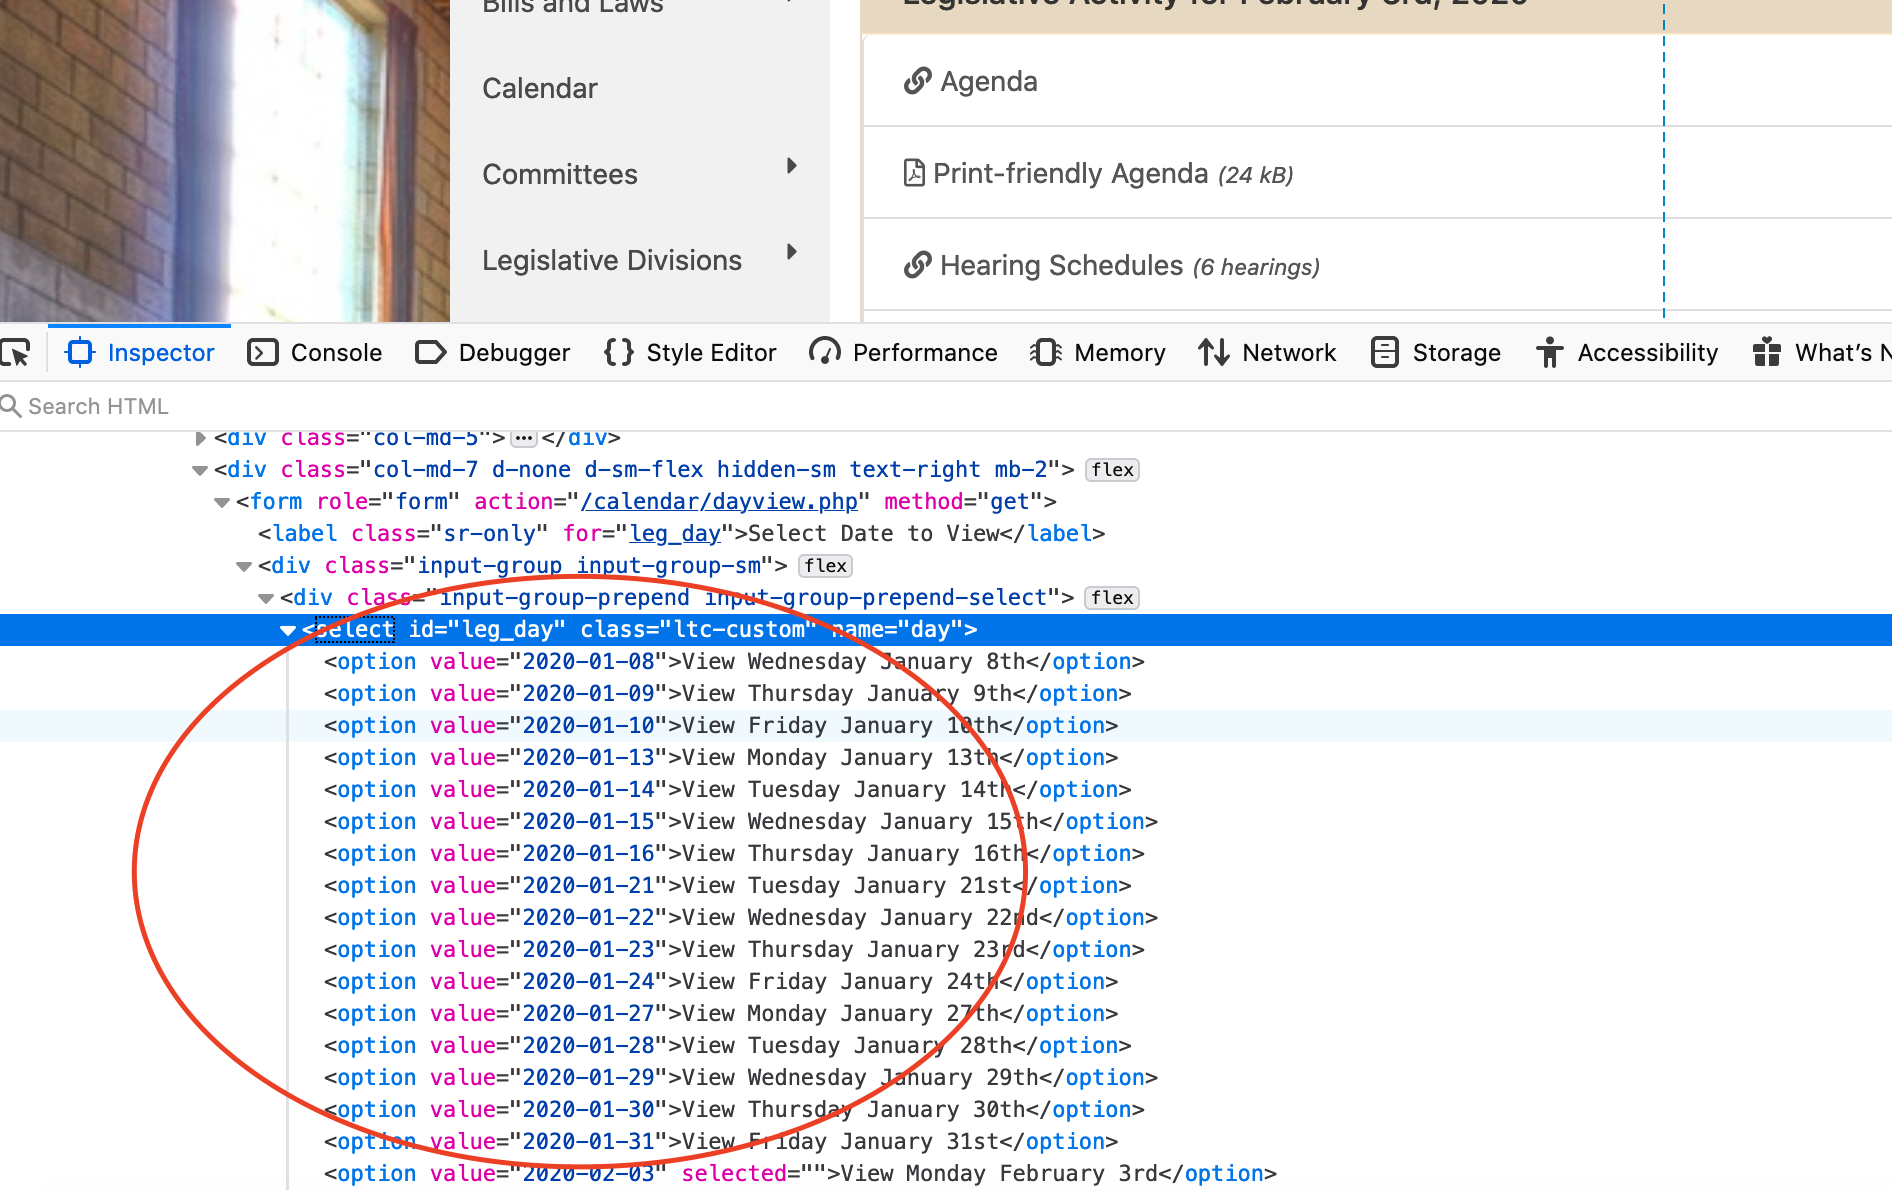
\includegraphics[width=26.28in]{images/advrvest1}

If it's HTML in the page, we can grab it, so let's do that. We start with the URL to any day, really.

\begin{Shaded}
\begin{Highlighting}[]
\NormalTok{url <-}\StringTok{ "https://nebraskalegislature.gov/calendar/dayview.php?day=2020-02-03"}
\end{Highlighting}
\end{Shaded}

I'm going to create a thing called a calendar and store the list of option values in there. So when I'm done, I'll have a list of dates.

\begin{Shaded}
\begin{Highlighting}[]
\NormalTok{calendar <-}\StringTok{ }\NormalTok{url }\OperatorTok
\StringTok{  }\KeywordTok{read_html}\NormalTok{() }\OperatorTok
\StringTok{  }\KeywordTok{html_nodes}\NormalTok{(}\DataTypeTok{xpath =} \StringTok{'//*[@id="leg_day"]'}\NormalTok{) }\OperatorTok
\StringTok{  }\KeywordTok{html_nodes}\NormalTok{(}\StringTok{"option"}\NormalTok{) }\OperatorTok
\StringTok{  }\KeywordTok{html_attrs}\NormalTok{()}
\end{Highlighting}
\end{Shaded}

\begin{Shaded}
\begin{Highlighting}[]
\NormalTok{calendar[}\DecValTok{1}\NormalTok{][}\DecValTok{1}\NormalTok{]}
\end{Highlighting}
\end{Shaded}

\begin{verbatim}
## [[1]]
##        value 
## "2020-01-08"
\end{verbatim}

Now this part gets tough, but if you follow, it's logical. It's step by step, really.

First, I noticed at the top of the agenda pages is a link to the daily agenda in csv format. Convenient, that.

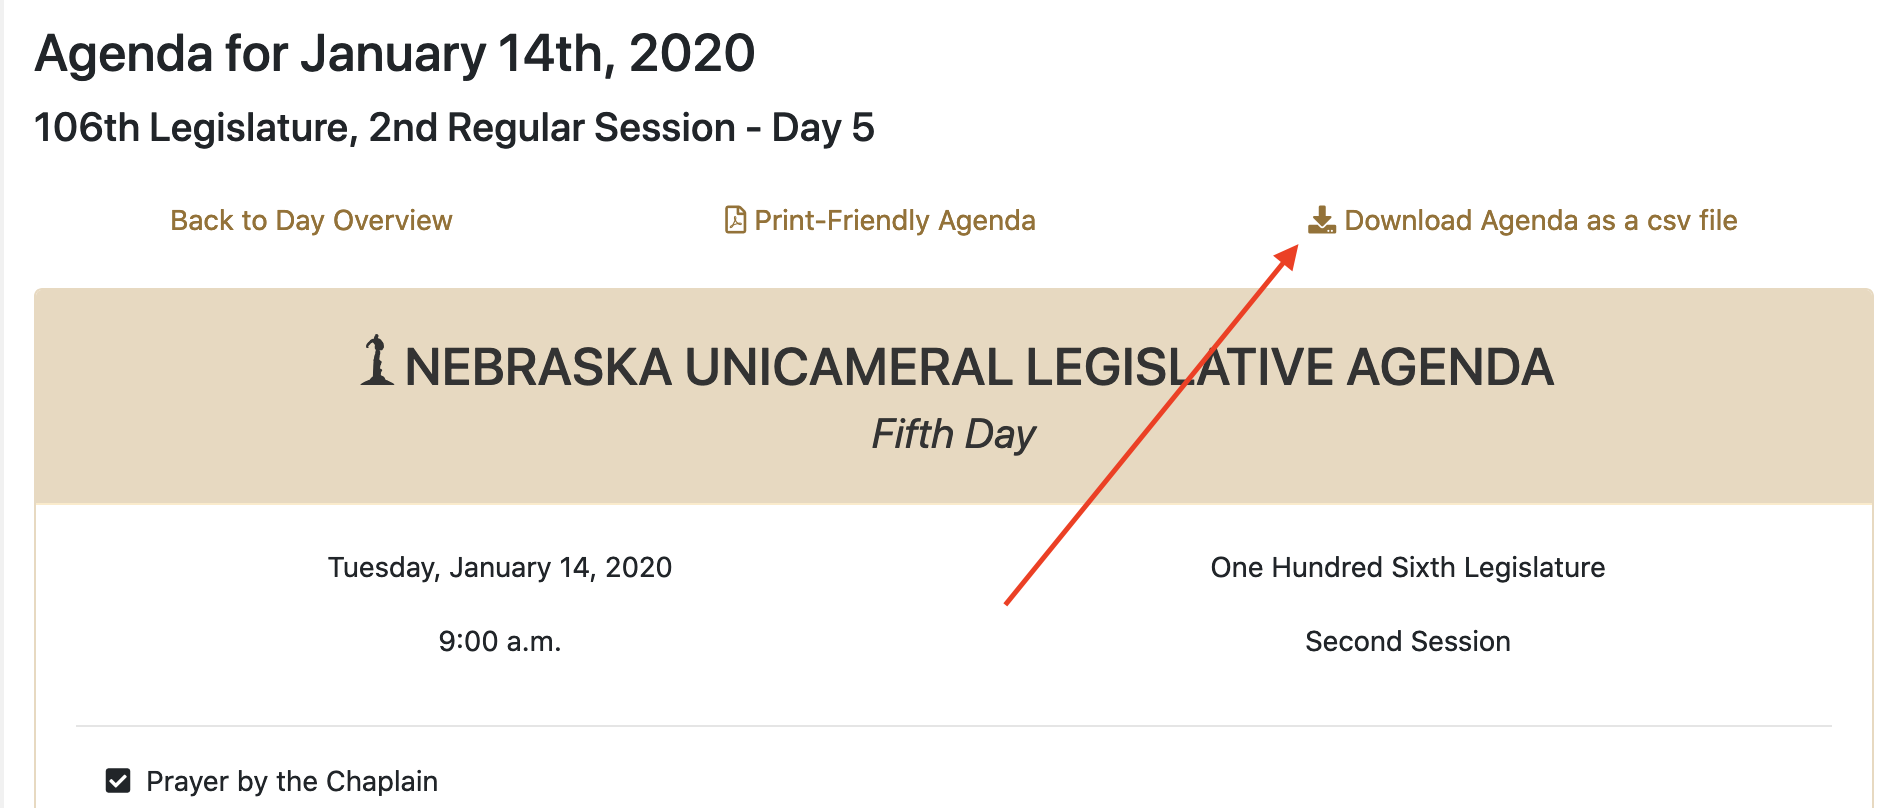
\includegraphics[width=26.39in]{images/advrvest2}

If you look at that url, it looks like this:

\begin{verbatim}
https://nebraskalegislature.gov/calendar/agenda.php?day=2020-01-14&print=csv
\end{verbatim}

If we can change the date in that url to each day of the session, we'd get a csv file for each day of the session that we can merge together.

Let's break down the steps to do that.

\begin{enumerate}
\def\labelenumi{\arabic{enumi}.}
\tightlist
\item
  I need a place to store this. A lazy way? Just import a day, filter everything out of it, and I've got an empty table I can \texttt{rbind} stuff into.
\item
  I need to set up a loop. For each day in the calendar, do some stuff.
\item
  I need to clean out the word selected (an HTML thing) from one of the dates.
\item
  I need to just scrape days that have business pending on the floor. So I can skip the first few days and I can skip any days into the future.
\item
  I need to take my date from calendar and add them to the url. Then I need to take that agenda url and add the csv parts.
\item
  Then I can use read\_csv like we have been to read the CSV url directly.
\item
  Then I just rbind my new csv to the one I created.
\item
  This isn't going to work perfectly every time, so I'm going to add some \texttt{tryCatch} statements that say try this, and if it doesn't work, do nothing.
\item
  Then, because I'm a decent fellow, I'm going to pause my query for three seconds to give their servers a break.
\end{enumerate}

Let's run it.

\begin{Shaded}
\begin{Highlighting}[]
\NormalTok{allbills <-}\StringTok{ }\KeywordTok{read_csv}\NormalTok{(}\StringTok{"https://nebraskalegislature.gov/calendar/agenda.php?day=2020-01-14&print=csv"}\NormalTok{, }\DataTypeTok{col_types =} \KeywordTok{cols}\NormalTok{()) }\OperatorTok\StringTok{ }\KeywordTok{mutate}\NormalTok{(}\DataTypeTok{Date =} \KeywordTok{as.Date}\NormalTok{(}\StringTok{"2020-01-01"}\NormalTok{))}\OperatorTok\StringTok{ }\KeywordTok{filter}\NormalTok{(}\StringTok{`}\DataTypeTok{Section Header}\StringTok{`} \OperatorTok{==}\StringTok{ "Blah"}\NormalTok{)}

\ControlFlowTok{for}\NormalTok{ (i }\ControlFlowTok{in}\NormalTok{ calendar)\{}
\NormalTok{  date <-}\StringTok{ }\NormalTok{i[}\DecValTok{1}\NormalTok{]}
\NormalTok{  checkdate <-}\StringTok{ }\KeywordTok{as.Date}\NormalTok{(date)}
  
  \ControlFlowTok{if}\NormalTok{ (checkdate }\OperatorTok{<=}\StringTok{ }\KeywordTok{Sys.Date}\NormalTok{() }\OperatorTok{&}\StringTok{ }\NormalTok{checkdate }\OperatorTok{>}\StringTok{ }\KeywordTok{as.Date}\NormalTok{(}\StringTok{"2020-01-13"}\NormalTok{)) \{}

\NormalTok{    agendaurl <-}\StringTok{ }\KeywordTok{paste}\NormalTok{(}\StringTok{"https://nebraskalegislature.gov/calendar/agenda.php?day="}\NormalTok{, i, }\DataTypeTok{sep=}\StringTok{""}\NormalTok{)}
\NormalTok{    csvurl <-}\KeywordTok{paste}\NormalTok{(agendaurl, }\StringTok{"&print=csv"}\NormalTok{, }\DataTypeTok{sep=}\StringTok{""}\NormalTok{)}
  \KeywordTok{tryCatch}\NormalTok{(}
\NormalTok{    agenda <-}\StringTok{ }\KeywordTok{read_csv}\NormalTok{(csvurl, }\DataTypeTok{col_types =} \KeywordTok{cols}\NormalTok{()) }\OperatorTok\StringTok{ }\KeywordTok{mutate}\NormalTok{(}\DataTypeTok{Date =}\NormalTok{ checkdate), }
    \DataTypeTok{error =} \ControlFlowTok{function}\NormalTok{(e)\{}\OtherTok{NA}\NormalTok{\})}
  \KeywordTok{tryCatch}\NormalTok{(}
\NormalTok{    allbills <-}\StringTok{ }\KeywordTok{rbind}\NormalTok{(allbills, agenda), }
    \DataTypeTok{error =} \ControlFlowTok{function}\NormalTok{(e)\{}\OtherTok{NA}\NormalTok{\})}
  \KeywordTok{Sys.sleep}\NormalTok{(}\DecValTok{3}\NormalTok{)}
\NormalTok{  \}}
\NormalTok{\}}
\end{Highlighting}
\end{Shaded}

\begin{verbatim}
## Warning: 2 parsing failures.
## row      col           expected actual                                                                           file
##  31 Oneliner delimiter or quote      C 'https://nebraskalegislature.gov/calendar/agenda.php?day=2020-03-06&print=csv'
##  31 Oneliner delimiter or quote        'https://nebraskalegislature.gov/calendar/agenda.php?day=2020-03-06&print=csv'
\end{verbatim}

And after that, I have a dataset of entries of bills on the floor. So if I want to see who has had the most bills on the floor -- including repeats -- I could answer that now.

\begin{Shaded}
\begin{Highlighting}[]
\NormalTok{allbills }\OperatorTok\StringTok{ }\KeywordTok{group_by}\NormalTok{(Introducer) }\OperatorTok\StringTok{ }\KeywordTok{tally}\NormalTok{(}\DataTypeTok{sort=}\OtherTok{TRUE}\NormalTok{) }\OperatorTok\StringTok{ }\KeywordTok{na.omit}\NormalTok{() }\OperatorTok\StringTok{ }\KeywordTok{top_n}\NormalTok{(}\DecValTok{5}\NormalTok{)}
\end{Highlighting}
\end{Shaded}

\begin{verbatim}
## Selecting by n
\end{verbatim}

\begin{verbatim}
## # A tibble: 5 x 2
##   Introducer         n
##   <chr>          <int>
## 1 Kolterman         46
## 2 Pansing Brooks    35
## 3 Vargas            35
## 4 Bolz              23
## 5 Stinner           22
\end{verbatim}

Senator Kolterman, collect your prize.

A note about advanced scraping -- every site is different. Every time you want to scrape a site, you'll be puzzling over different problems. But the steps remain the same: find a pattern, exploit it, clean the data on the fly and put it into a place to store it.

\hypertarget{intro-to-apis-the-census}{%
\chapter{Intro to APIs: The Census}\label{intro-to-apis-the-census}}

There is truly an astonishing amount of data collected by the US Census Bureau. First, there's the Census that most people know -- the every 10 year census. That's the one mandated by the Constitution where the government attempts to count every person in the US. It's a mind-boggling feat to even try, and billions get spent on it. That data is used first for determining how many representatives each state gets in Congress. From there, the Census gets used to divide up billions of dollars of federal spending.

To answer the questions the government needs to do that, a ton of data gets collected. That, unfortunately, means the Census is exceedingly complicated to work with. The good news is, the Census has an API -- an application programming interface. What that means is we can get data directly through the Census Bureau via calls over the internet.

Let's demonstrate.

We're going to use a library called \texttt{tidycensus} which makes calls to the Census API in a very tidy way, and gives you back tidy data. That means we don't have to go through the process of importing the data from a file. I can't tell you how amazing this is, speaking from experience.

First we need to install \texttt{tidycensus} using the console: \texttt{install.packages("tidycensus")}

\begin{Shaded}
\begin{Highlighting}[]
\KeywordTok{library}\NormalTok{(tidyverse)}
\KeywordTok{library}\NormalTok{(tidycensus)}
\end{Highlighting}
\end{Shaded}

To use the API, you need an API key. To get that, you need to \href{https://api.census.gov/data/key_signup.html}{apply for an API key with the Census Bureau}. It takes a few minutes and you need to activate your key via email. Once you have your key, you need to set that for this session:

\begin{verbatim}
census_api_key("YOUR KEY HERE")
\end{verbatim}

Just FYI: Your key is your key. Do not share it around.

\begin{verbatim}
## To install your API key for use in future sessions, run this function with `install = TRUE`.
\end{verbatim}

So to give you some idea of how complicated the data is, let's pull up just one file from the decennial Census. We'll use Summary File 1, or SF1. That has the major population and housing stuff.

\begin{Shaded}
\begin{Highlighting}[]
\NormalTok{sf1 <-}\StringTok{ }\KeywordTok{load_variables}\NormalTok{(}\DecValTok{2010}\NormalTok{, }\StringTok{"sf1"}\NormalTok{, }\DataTypeTok{cache =} \OtherTok{TRUE}\NormalTok{)}
\end{Highlighting}
\end{Shaded}

Note: There are 3,346 variables in SF1. That's not a typo. Open it in your environment by double clicking. As you scroll down, you'll get an idea of what you've got to choose from.

If you think that's crazy, try the SF3 file from 2000.

\begin{Shaded}
\begin{Highlighting}[]
\NormalTok{sf3 <-}\StringTok{ }\KeywordTok{load_variables}\NormalTok{(}\DecValTok{2000}\NormalTok{, }\StringTok{"sf3"}\NormalTok{, }\DataTypeTok{cache =} \OtherTok{TRUE}\NormalTok{)}
\end{Highlighting}
\end{Shaded}

Yes. That's 5,555 variables to choose from. I told you. Astonishing.

So let's try to answer a question using the Census. What is the fastest growing state since 1990?

To answer this, we need to pull the total population by state in each of the decennial census. Here's 1990.

\begin{Shaded}
\begin{Highlighting}[]
\NormalTok{p90 <-}\StringTok{ }\KeywordTok{get_decennial}\NormalTok{(}\DataTypeTok{geography =} \StringTok{"state"}\NormalTok{, }\DataTypeTok{variables =} \StringTok{"P0010001"}\NormalTok{, }\DataTypeTok{year =} \DecValTok{1990}\NormalTok{)}
\end{Highlighting}
\end{Shaded}

\begin{verbatim}
## Getting data from the 1990 decennial Census
\end{verbatim}

Now 2000.

\begin{Shaded}
\begin{Highlighting}[]
\NormalTok{p00 <-}\StringTok{ }\KeywordTok{get_decennial}\NormalTok{(}\DataTypeTok{geography =} \StringTok{"state"}\NormalTok{, }\DataTypeTok{variables =} \StringTok{"P001001"}\NormalTok{, }\DataTypeTok{year =} \DecValTok{2000}\NormalTok{)}
\end{Highlighting}
\end{Shaded}

\begin{verbatim}
## Getting data from the 2000 decennial Census
\end{verbatim}

Now 2010.

\begin{Shaded}
\begin{Highlighting}[]
\NormalTok{p10 <-}\StringTok{ }\KeywordTok{get_decennial}\NormalTok{(}\DataTypeTok{geography =} \StringTok{"state"}\NormalTok{, }\DataTypeTok{variables =} \StringTok{"P001001"}\NormalTok{, }\DataTypeTok{year =} \DecValTok{2010}\NormalTok{)}
\end{Highlighting}
\end{Shaded}

\begin{verbatim}
## Getting data from the 2010 decennial Census
\end{verbatim}

Let's take a peek at 2010.

\begin{Shaded}
\begin{Highlighting}[]
\NormalTok{p10}
\end{Highlighting}
\end{Shaded}

\begin{verbatim}
## # A tibble: 52 x 4
##    GEOID NAME        variable    value
##    <chr> <chr>       <chr>       <dbl>
##  1 01    Alabama     P001001   4779736
##  2 02    Alaska      P001001    710231
##  3 04    Arizona     P001001   6392017
##  4 05    Arkansas    P001001   2915918
##  5 06    California  P001001  37253956
##  6 22    Louisiana   P001001   4533372
##  7 21    Kentucky    P001001   4339367
##  8 08    Colorado    P001001   5029196
##  9 09    Connecticut P001001   3574097
## 10 10    Delaware    P001001    897934
## # ... with 42 more rows
\end{verbatim}

As you can see, we have a GEOID, NAME, then variable and value. Variable and value are going to be the same. Because those are named the same thing, to merge them together, we need to rename them.

\begin{Shaded}
\begin{Highlighting}[]
\NormalTok{p10 }\OperatorTok\StringTok{ }\KeywordTok{select}\NormalTok{(GEOID, NAME, value) }\OperatorTok\StringTok{ }\KeywordTok{rename}\NormalTok{(}\DataTypeTok{Population2010=}\NormalTok{value) ->}\StringTok{ }\NormalTok{p2010}

\NormalTok{p00 }\OperatorTok\StringTok{ }\KeywordTok{select}\NormalTok{(GEOID, NAME, value) }\OperatorTok\StringTok{ }\KeywordTok{rename}\NormalTok{(}\DataTypeTok{Population2000=}\NormalTok{value) ->}\StringTok{ }\NormalTok{p2000}

\NormalTok{p90 }\OperatorTok\StringTok{ }\KeywordTok{select}\NormalTok{(GEOID, NAME, value) }\OperatorTok\StringTok{ }\KeywordTok{rename}\NormalTok{(}\DataTypeTok{Population1990=}\NormalTok{value) ->}\StringTok{ }\NormalTok{p1990}
\end{Highlighting}
\end{Shaded}

Now we join the data together.

\begin{Shaded}
\begin{Highlighting}[]
\NormalTok{alldata <-}\StringTok{ }\NormalTok{p1990 }\OperatorTok\StringTok{ }\KeywordTok{inner_join}\NormalTok{(p2000) }\OperatorTok\StringTok{ }\KeywordTok{inner_join}\NormalTok{(p2010)}
\end{Highlighting}
\end{Shaded}

\begin{verbatim}
## Joining, by = c("GEOID", "NAME")Joining, by = c("GEOID", "NAME")
\end{verbatim}

And now we calculate the percent change.

\begin{Shaded}
\begin{Highlighting}[]
\NormalTok{alldata }\OperatorTok\StringTok{ }\KeywordTok{mutate}\NormalTok{(}\DataTypeTok{change =}\NormalTok{ ((Population2010}\OperatorTok{-}\NormalTok{Population1990)}\OperatorTok{/}\NormalTok{Population1990)}\OperatorTok{*}\DecValTok{100}\NormalTok{) }\OperatorTok\StringTok{ }\KeywordTok{arrange}\NormalTok{(}\KeywordTok{desc}\NormalTok{(change))}
\end{Highlighting}
\end{Shaded}

\begin{verbatim}
## # A tibble: 51 x 6
##    GEOID NAME           Population1990 Population2000 Population2010 change
##    <chr> <chr>                   <dbl>          <dbl>          <dbl>  <dbl>
##  1 32    Nevada                1201833        1998257        2700551  125. 
##  2 04    Arizona               3665228        5130632        6392017   74.4
##  3 49    Utah                  1722850        2233169        2763885   60.4
##  4 16    Idaho                 1006749        1293953        1567582   55.7
##  5 08    Colorado              3294394        4301261        5029196   52.7
##  6 13    Georgia               6478216        8186453        9687653   49.5
##  7 48    Texas                16986510       20851820       25145561   48.0
##  8 12    Florida              12937926       15982378       18801310   45.3
##  9 37    North Carolina        6628637        8049313        9535483   43.9
## 10 53    Washington            4866692        5894121        6724540   38.2
## # ... with 41 more rows
\end{verbatim}

And just like that: Nevada. Nebraska is 33rd fastest growing.

\hypertarget{the-acs}{%
\section{The ACS}\label{the-acs}}

In 2010, the Census Bureau replaced SF3 with the American Community Survey. The Good News is that the data would be updated on a rolling basis. The bad news is that it's more complicated because it's more like survey data with a large sample. That means there's margins of error and confidence intervals to worry about.

Here's an example:

What is Nebraska's richest county?

We can measure this by median household income. That variable is \texttt{B19013\_001}, so we can get that data like this (I'm narrowing it to the top 20 for simplicity):

\begin{Shaded}
\begin{Highlighting}[]
\NormalTok{ne <-}\StringTok{ }\KeywordTok{get_acs}\NormalTok{(}\DataTypeTok{geography =} \StringTok{"county"}\NormalTok{, }
              \DataTypeTok{variables =} \KeywordTok{c}\NormalTok{(}\DataTypeTok{medincome =} \StringTok{"B19013_001"}\NormalTok{), }
              \DataTypeTok{state =} \StringTok{"NE"}\NormalTok{, }
              \DataTypeTok{year =} \DecValTok{2018}\NormalTok{)}
\end{Highlighting}
\end{Shaded}

\begin{verbatim}
## Getting data from the 2014-2018 5-year ACS
\end{verbatim}

\begin{Shaded}
\begin{Highlighting}[]
\NormalTok{ne <-}\StringTok{ }\NormalTok{ne }\OperatorTok\StringTok{ }\KeywordTok{arrange}\NormalTok{(}\KeywordTok{desc}\NormalTok{(estimate)) }\OperatorTok\StringTok{ }\KeywordTok{top_n}\NormalTok{(}\DecValTok{20}\NormalTok{, estimate)}

\NormalTok{ne}
\end{Highlighting}
\end{Shaded}

\begin{verbatim}
## # A tibble: 21 x 5
##    GEOID NAME                        variable  estimate   moe
##    <chr> <chr>                       <chr>        <dbl> <dbl>
##  1 31153 Sarpy County, Nebraska      medincome    79549  1419
##  2 31025 Cass County, Nebraska       medincome    71139  2310
##  3 31177 Washington County, Nebraska medincome    70753  3504
##  4 31159 Seward County, Nebraska     medincome    67591  3082
##  5 31155 Saunders County, Nebraska   medincome    66718  3394
##  6 31081 Hamilton County, Nebraska   medincome    64042  3775
##  7 31167 Stanton County, Nebraska    medincome    62687  4761
##  8 31179 Wayne County, Nebraska      medincome    62623  8752
##  9 31141 Platte County, Nebraska     medincome    62617  3413
## 10 31073 Gosper County, Nebraska     medincome    62545  3065
## # ... with 11 more rows
\end{verbatim}

Sarpy, Cass, Washington. What do they all have in common? They ring Douglas County -- Omaha. So lots of suburban flight. But do the margins of error let us say one county is richer than the other. We can find this out visually using error bars. Don't worry much about the code here -- we'll cover that soon enough.

\begin{Shaded}
\begin{Highlighting}[]
\NormalTok{ne }\OperatorTok
\StringTok{  }\KeywordTok{mutate}\NormalTok{(}\DataTypeTok{NAME =} \KeywordTok{gsub}\NormalTok{(}\StringTok{" County, Nebraska"}\NormalTok{, }\StringTok{""}\NormalTok{, NAME)) }\OperatorTok
\StringTok{  }\KeywordTok{ggplot}\NormalTok{(}\KeywordTok{aes}\NormalTok{(}\DataTypeTok{x =}\NormalTok{ estimate, }\DataTypeTok{y =} \KeywordTok{reorder}\NormalTok{(NAME, estimate))) }\OperatorTok{+}
\StringTok{  }\KeywordTok{geom_errorbarh}\NormalTok{(}\KeywordTok{aes}\NormalTok{(}\DataTypeTok{xmin =}\NormalTok{ estimate }\OperatorTok{-}\StringTok{ }\NormalTok{moe, }\DataTypeTok{xmax =}\NormalTok{ estimate }\OperatorTok{+}\StringTok{ }\NormalTok{moe)) }\OperatorTok{+}
\StringTok{  }\KeywordTok{geom_point}\NormalTok{(}\DataTypeTok{color =} \StringTok{"red"}\NormalTok{) }\OperatorTok{+}
\StringTok{  }\KeywordTok{labs}\NormalTok{(}\DataTypeTok{title =} \StringTok{"Household income by county in Nebraska"}\NormalTok{,}
       \DataTypeTok{subtitle =} \StringTok{"2013-2017 American Community Survey"}\NormalTok{,}
       \DataTypeTok{y =} \StringTok{""}\NormalTok{,}
       \DataTypeTok{x =} \StringTok{"ACS estimate (bars represent margin of error)"}\NormalTok{)}
\end{Highlighting}
\end{Shaded}

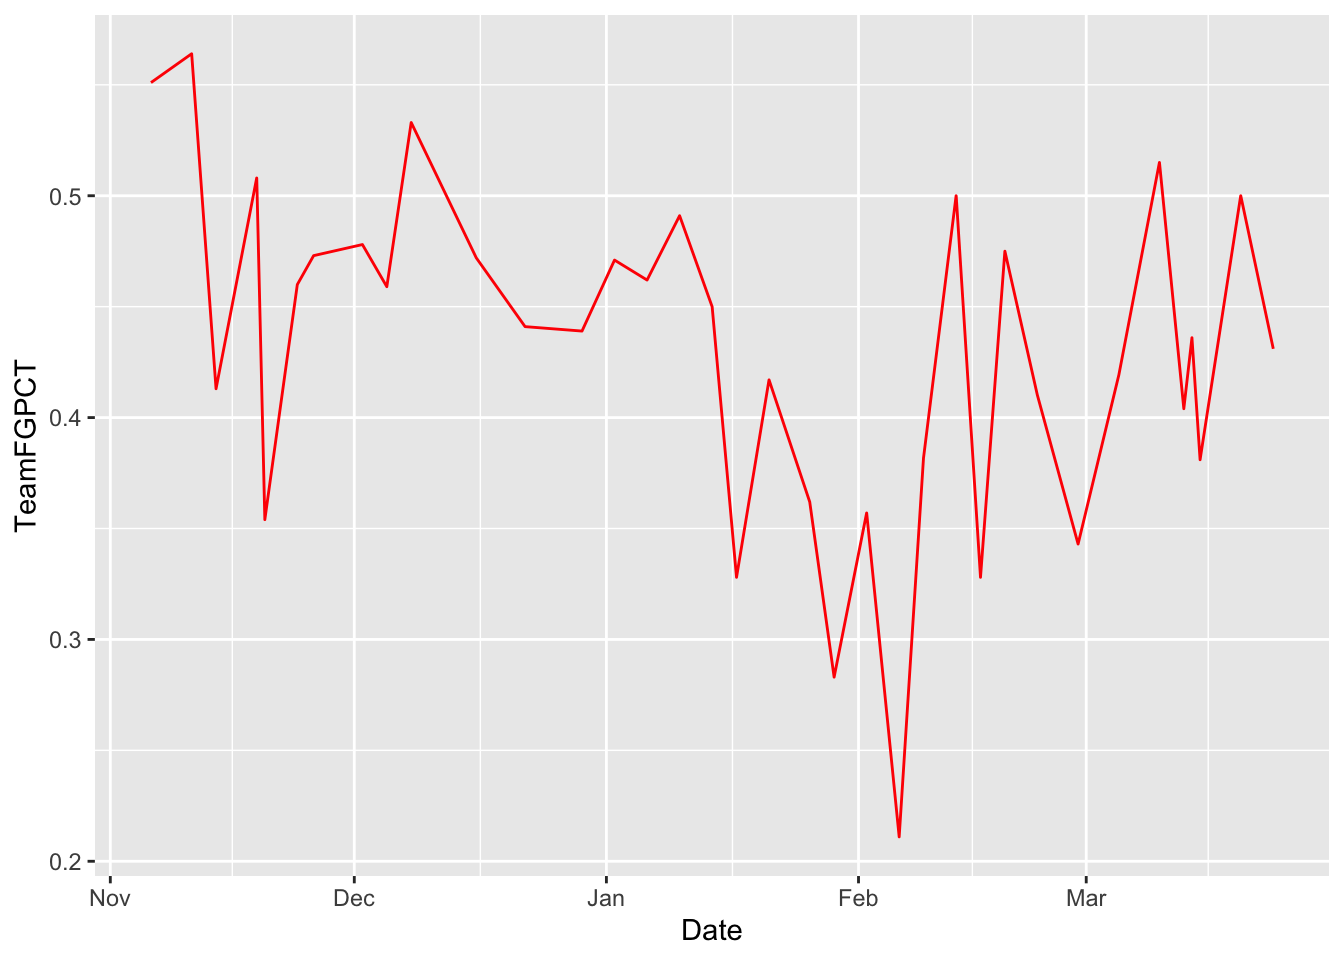
\includegraphics{datajournalism_files/figure-latex/unnamed-chunk-139-1.pdf}

As you can see, some of the error bars are quite wide. Some are narrow. But if the bars overlap, it means the difference between the two counties is within the margin of error, and the differences aren't statistically significant. So is the difference between Cass and Washington significant? Nope. Is the difference between Sarpy and everyone else significant? Yes it is.

Let's ask another question of the ACS -- did any counties lose income from the time of the global financial crisis to the current 5-year window?

Let's re-label our first household income data.

\begin{Shaded}
\begin{Highlighting}[]
\NormalTok{ne18 <-}\StringTok{ }\KeywordTok{get_acs}\NormalTok{(}\DataTypeTok{geography =} \StringTok{"county"}\NormalTok{, }
              \DataTypeTok{variables =} \KeywordTok{c}\NormalTok{(}\DataTypeTok{medincome =} \StringTok{"B19013_001"}\NormalTok{), }
              \DataTypeTok{state =} \StringTok{"NE"}\NormalTok{, }
              \DataTypeTok{year =} \DecValTok{2018}\NormalTok{)}
\end{Highlighting}
\end{Shaded}

\begin{verbatim}
## Getting data from the 2014-2018 5-year ACS
\end{verbatim}

And now we grab the 2010 median household income.

\begin{Shaded}
\begin{Highlighting}[]
\NormalTok{ne10 <-}\StringTok{ }\KeywordTok{get_acs}\NormalTok{(}\DataTypeTok{geography =} \StringTok{"county"}\NormalTok{, }
              \DataTypeTok{variables =} \KeywordTok{c}\NormalTok{(}\DataTypeTok{medincome =} \StringTok{"B19013_001"}\NormalTok{), }
              \DataTypeTok{state =} \StringTok{"NE"}\NormalTok{, }
              \DataTypeTok{year =} \DecValTok{2010}\NormalTok{)}
\end{Highlighting}
\end{Shaded}

\begin{verbatim}
## Getting data from the 2006-2010 5-year ACS
\end{verbatim}

What I'm going to do next is a lot, but each step is simple. I'm going to join the data together, so each county has one line of data. Then I'm going to rename some fields that repeat. Then I'm going to calculate the minimium and maximum value of the estimate using the margin of error. That'll help me later. After that, I'm going to calculate a perent change and sort it by that change.

\begin{Shaded}
\begin{Highlighting}[]
\NormalTok{ne10 }\OperatorTok\StringTok{ }
\StringTok{  }\KeywordTok{inner_join}\NormalTok{(ne18, }\DataTypeTok{by=}\KeywordTok{c}\NormalTok{(}\StringTok{"GEOID"}\NormalTok{, }\StringTok{"NAME"}\NormalTok{)) }\OperatorTok\StringTok{ }
\StringTok{  }\KeywordTok{rename}\NormalTok{(}\DataTypeTok{estimate2010=}\NormalTok{estimate.x, }\DataTypeTok{estimate2018=}\NormalTok{estimate.y) }\OperatorTok\StringTok{ }
\StringTok{  }\KeywordTok{mutate}\NormalTok{(}\DataTypeTok{min2010 =}\NormalTok{ estimate2010}\OperatorTok{-}\NormalTok{moe.x, }\DataTypeTok{max2010 =}\NormalTok{ estimate2010}\OperatorTok{+}\NormalTok{moe.x, }\DataTypeTok{min2018 =}\NormalTok{ estimate2018}\OperatorTok{-}\NormalTok{moe.y, }\DataTypeTok{max2018 =}\NormalTok{ estimate2018}\OperatorTok{+}\NormalTok{moe.y) }\OperatorTok\StringTok{ }
\StringTok{  }\KeywordTok{select}\NormalTok{(}\OperatorTok{-}\NormalTok{variable.x, }\OperatorTok{-}\NormalTok{variable.y, }\OperatorTok{-}\NormalTok{moe.x, }\OperatorTok{-}\NormalTok{moe.y) }\OperatorTok\StringTok{ }
\StringTok{  }\KeywordTok{mutate}\NormalTok{(}\DataTypeTok{change =}\NormalTok{ ((estimate2018}\OperatorTok{-}\NormalTok{estimate2010)}\OperatorTok{/}\NormalTok{estimate2010)}\OperatorTok{*}\DecValTok{100}\NormalTok{) }\OperatorTok\StringTok{ }
\StringTok{  }\KeywordTok{arrange}\NormalTok{(change)}
\end{Highlighting}
\end{Shaded}

\begin{verbatim}
## # A tibble: 93 x 9
##    GEOID NAME   estimate2010 estimate2018 min2010 max2010 min2018 max2018 change
##    <chr> <chr>         <dbl>        <dbl>   <dbl>   <dbl>   <dbl>   <dbl>  <dbl>
##  1 31117 McPhe~        50625        48882   38979   62271   41666   56098 -3.44 
##  2 31085 Hayes~        45595        45515   41833   49357   38687   52343 -0.175
##  3 31075 Grant~        39261        39479   35341   43181   27482   51476  0.555
##  4 31091 Hooke~        38750        39115   28329   49171   33409   44821  0.942
##  5 31005 Arthu~        43250        43854   33524   52976   40943   46765  1.40 
##  6 31095 Jeffe~        42665        43295   38489   46841   39615   46975  1.48 
##  7 31105 Kimba~        42010        43856   36672   47348   39378   48334  4.39 
##  8 31099 Kearn~        54518        56952   50397   58639   51557   62347  4.46 
##  9 31171 Thoma~        48250        50682   41698   54802   43155   58209  5.04 
## 10 31125 Nance~        41610        45833   39073   44147   40753   50913 10.1  
## # ... with 83 more rows
\end{verbatim}

So according to this, McPherson and Hayes counties lost ground from the financial meltdown to now.

But did they?

Look at the min and max values for both. Is the change statistically significant?

\hypertarget{bonus-api-example-coronavirus}{%
\section{Bonus API example: Coronavirus}\label{bonus-api-example-coronavirus}}

As I'm writing this, there is a growing level of fear about the novel coronavirus, COVID-19. And, as I'm writing this, I was alerted to a new R package that pulls daily updates of coronavirus reports daily. You install it with \texttt{install.packages("coronavirus")}

\begin{Shaded}
\begin{Highlighting}[]
\KeywordTok{library}\NormalTok{(coronavirus)}

\KeywordTok{data}\NormalTok{(}\StringTok{"coronavirus"}\NormalTok{) }
\end{Highlighting}
\end{Shaded}

What just happened, without you having to do anything, is the library just made a call to servers at Johns Hopkins University and got the latest coronavirus numbers from around the world.

Check it out:

\begin{Shaded}
\begin{Highlighting}[]
\KeywordTok{view}\NormalTok{(coronavirus)}
\end{Highlighting}
\end{Shaded}

So now we can start using it for data analysis. How about cases in the US?

\begin{Shaded}
\begin{Highlighting}[]
\NormalTok{coronavirus }\OperatorTok\StringTok{ }\KeywordTok{filter}\NormalTok{(Country.Region }\OperatorTok{==}\StringTok{ "US"}\NormalTok{)}
\end{Highlighting}
\end{Shaded}

\begin{verbatim}
## # A tibble: 16 x 7
##    Province.State       Country.Region   Lat   Long date       cases type     
##    <chr>                <chr>          <dbl>  <dbl> <date>     <int> <chr>    
##  1 Seattle, WA          US              47.8 -121.  2020-01-22     1 confirmed
##  2 Chicago, IL          US              40.6  -89.4 2020-01-24     1 confirmed
##  3 Los Angeles, CA      US              34.1 -118.  2020-01-26     1 confirmed
##  4 Orange, CA           US              33.8 -118.  2020-01-26     1 confirmed
##  5 Tempe, AZ            US              34.0 -111.  2020-01-26     1 confirmed
##  6 Chicago, IL          US              40.6  -89.4 2020-01-31     1 confirmed
##  7 Santa Clara, CA      US              37.4 -122.  2020-01-31     1 confirmed
##  8 Boston, MA           US              42.4  -71.1 2020-02-01     1 confirmed
##  9 San Benito, CA       US              36.6 -121.  2020-02-03     2 confirmed
## 10 Santa Clara, CA      US              37.4 -122.  2020-02-03     1 confirmed
## 11 Madison, WI          US              43.1  -89.4 2020-02-05     1 confirmed
## 12 Chicago, IL          US              40.6  -89.4 2020-02-09     2 recovered
## 13 Seattle, WA          US              47.8 -121.  2020-02-09     1 recovered
## 14 San Diego County, CA US              32.7 -117.  2020-02-11     1 confirmed
## 15 San Antonio, TX      US              29.4  -98.5 2020-02-13     1 confirmed
## 16 San Diego County, CA US              32.7 -117.  2020-02-13     1 confirmed
\end{verbatim}

How about confirmed cases by country?

\begin{Shaded}
\begin{Highlighting}[]
\NormalTok{coronavirus }\OperatorTok\StringTok{ }\KeywordTok{filter}\NormalTok{(type }\OperatorTok{==}\StringTok{ "confirmed"}\NormalTok{) }\OperatorTok\StringTok{ }\KeywordTok{group_by}\NormalTok{(Country.Region) }\OperatorTok\StringTok{ }\KeywordTok{summarize}\NormalTok{(}\DataTypeTok{total=}\KeywordTok{sum}\NormalTok{(cases)) }\OperatorTok\StringTok{ }\KeywordTok{arrange}\NormalTok{(}\KeywordTok{desc}\NormalTok{(total))}
\end{Highlighting}
\end{Shaded}

\begin{verbatim}
## # A tibble: 30 x 2
##    Country.Region total
##    <chr>          <int>
##  1 Mainland China 70446
##  2 Others           355
##  3 Singapore         75
##  4 Japan             59
##  5 Hong Kong         57
##  6 Thailand          34
##  7 South Korea       29
##  8 Malaysia          22
##  9 Taiwan            20
## 10 Germany           16
## # ... with 20 more rows
\end{verbatim}

With this library, you could track this every day. Pretty neat, if you ask me.

\hypertarget{visualizing-your-data-for-reporting}{%
\chapter{Visualizing your data for reporting}\label{visualizing-your-data-for-reporting}}

Visualizing data is becoming a much greater part of journalism. Large news organizations are creating graphics desks that create complex visuals with data to inform the public about important events.

To do it well is a course on it's own. And not every story needs a feat of programming and art. Sometimes, you can help yourself and your story by just creating a quick chart.

Good news: one of the best libraries for visualizing data is in the tidyverse and it's pretty simple to make simple charts quickly with just a little bit of code.

Let's revisit some data we've used in the past and turn it into charts.

\begin{Shaded}
\begin{Highlighting}[]
\KeywordTok{library}\NormalTok{(tidyverse)}
\end{Highlighting}
\end{Shaded}

The dataset we'll use is \href{https://unl.box.com/s/xjipgkesl9rjmng4weg77vb73xt41apf}{the mountainlion data} we looked at in Chapter 6.

\begin{Shaded}
\begin{Highlighting}[]
\NormalTok{mountainlions <-}\StringTok{ }\KeywordTok{read_csv}\NormalTok{(}\StringTok{"data/mountainlions.csv"}\NormalTok{)}
\end{Highlighting}
\end{Shaded}

\begin{verbatim}
## Parsed with column specification:
## cols(
##   ID = col_double(),
##   `Cofirm Type` = col_character(),
##   COUNTY = col_character(),
##   Date = col_character()
## )
\end{verbatim}

\hypertarget{bar-charts}{%
\section{Bar charts}\label{bar-charts}}

The first kind of chart we'll create is a simple bar chart. It's a chart designed to show differences between things -- the magnitude of one, compared to the next, and the next, and the next. So if we have thing, like a county, or a state, or a group name, and then a count of that group, we can make a bar chart.

So what does the chart of the top 10 counties with the most mountain sightings look like?

First, we'll create a dataframe of those top 10, called topsightings.

\begin{Shaded}
\begin{Highlighting}[]
\NormalTok{mountainlions }\OperatorTok
\StringTok{  }\KeywordTok{group_by}\NormalTok{(COUNTY) }\OperatorTok
\StringTok{  }\KeywordTok{summarise}\NormalTok{(}
    \DataTypeTok{total =} \KeywordTok{n}\NormalTok{()}
\NormalTok{  ) }\OperatorTok\StringTok{ }\KeywordTok{top_n}\NormalTok{(}\DecValTok{10}\NormalTok{, total) ->}\StringTok{ }\NormalTok{topsightings}
\end{Highlighting}
\end{Shaded}

Now ggplot. The first thing we do with ggplot is invoke it, which creates the canvas. In ggplot, we work with geometries -- the shape that the data will take -- and aesthetics -- the data that will take shape. In a bar chart, we first pass in the data to the geometry, then set the aesthetic. We tell ggplot what the x value is -- in a bar chart, that's almost always your grouping variable. Then we tell it the weight of the bar -- the number that will set the height.

\begin{Shaded}
\begin{Highlighting}[]
\KeywordTok{ggplot}\NormalTok{() }\OperatorTok{+}\StringTok{ }\KeywordTok{geom_bar}\NormalTok{(}\DataTypeTok{data=}\NormalTok{topsightings, }\KeywordTok{aes}\NormalTok{(}\DataTypeTok{x=}\NormalTok{COUNTY, }\DataTypeTok{weight=}\NormalTok{total))}
\end{Highlighting}
\end{Shaded}

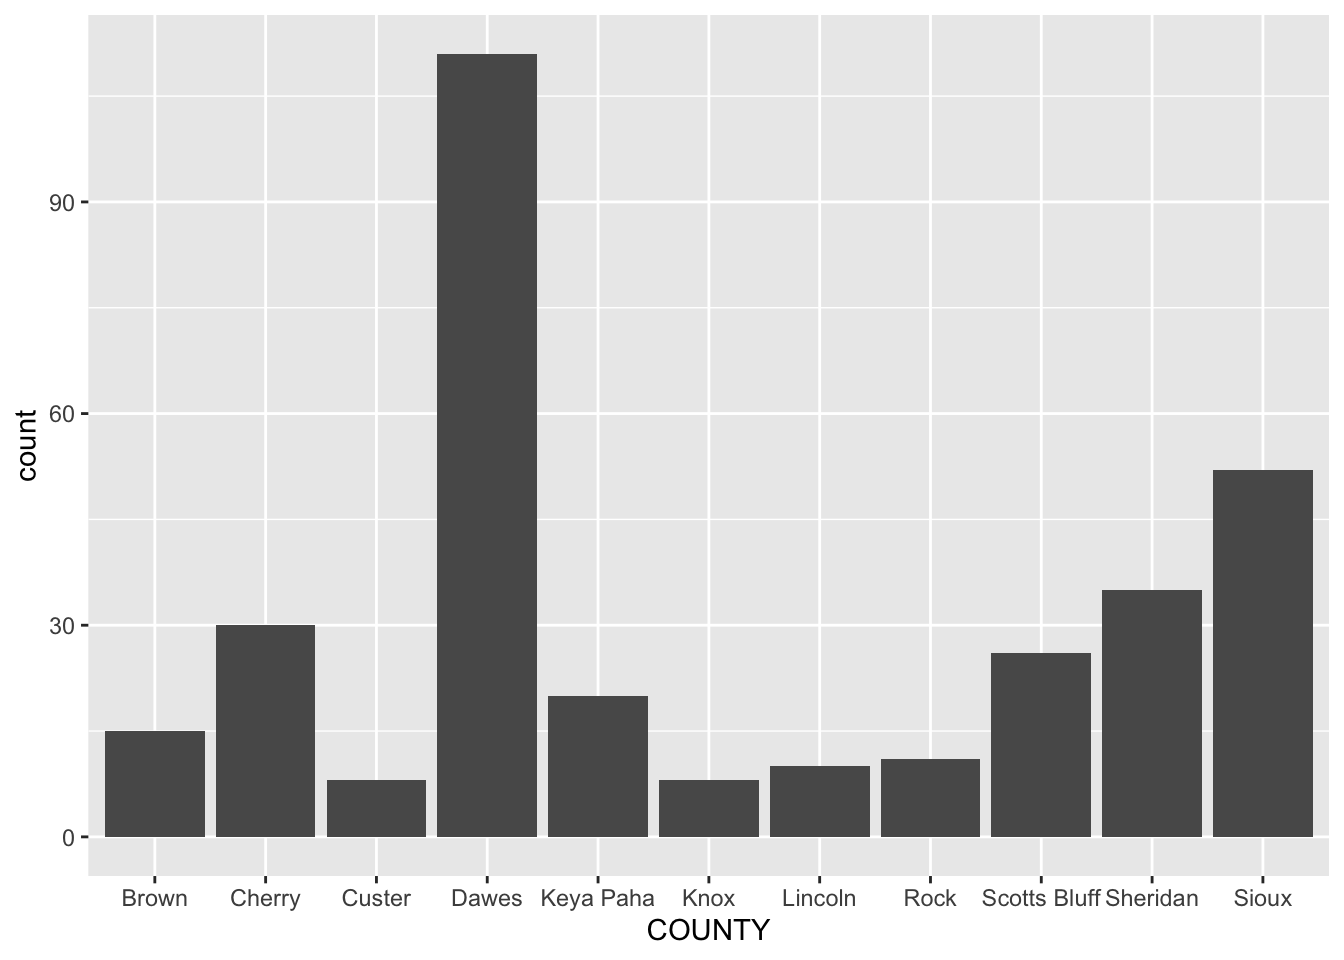
\includegraphics{datajournalism_files/figure-latex/unnamed-chunk-150-1.pdf}

The bars look good, but he order makes no sense. In ggplot, we use reorder, and we reorder the x value based on the weight, like this:

\begin{Shaded}
\begin{Highlighting}[]
\KeywordTok{ggplot}\NormalTok{() }\OperatorTok{+}\StringTok{ }\KeywordTok{geom_bar}\NormalTok{(}\DataTypeTok{data=}\NormalTok{topsightings, }\KeywordTok{aes}\NormalTok{(}\DataTypeTok{x=}\KeywordTok{reorder}\NormalTok{(COUNTY, total), }\DataTypeTok{weight=}\NormalTok{total))}
\end{Highlighting}
\end{Shaded}

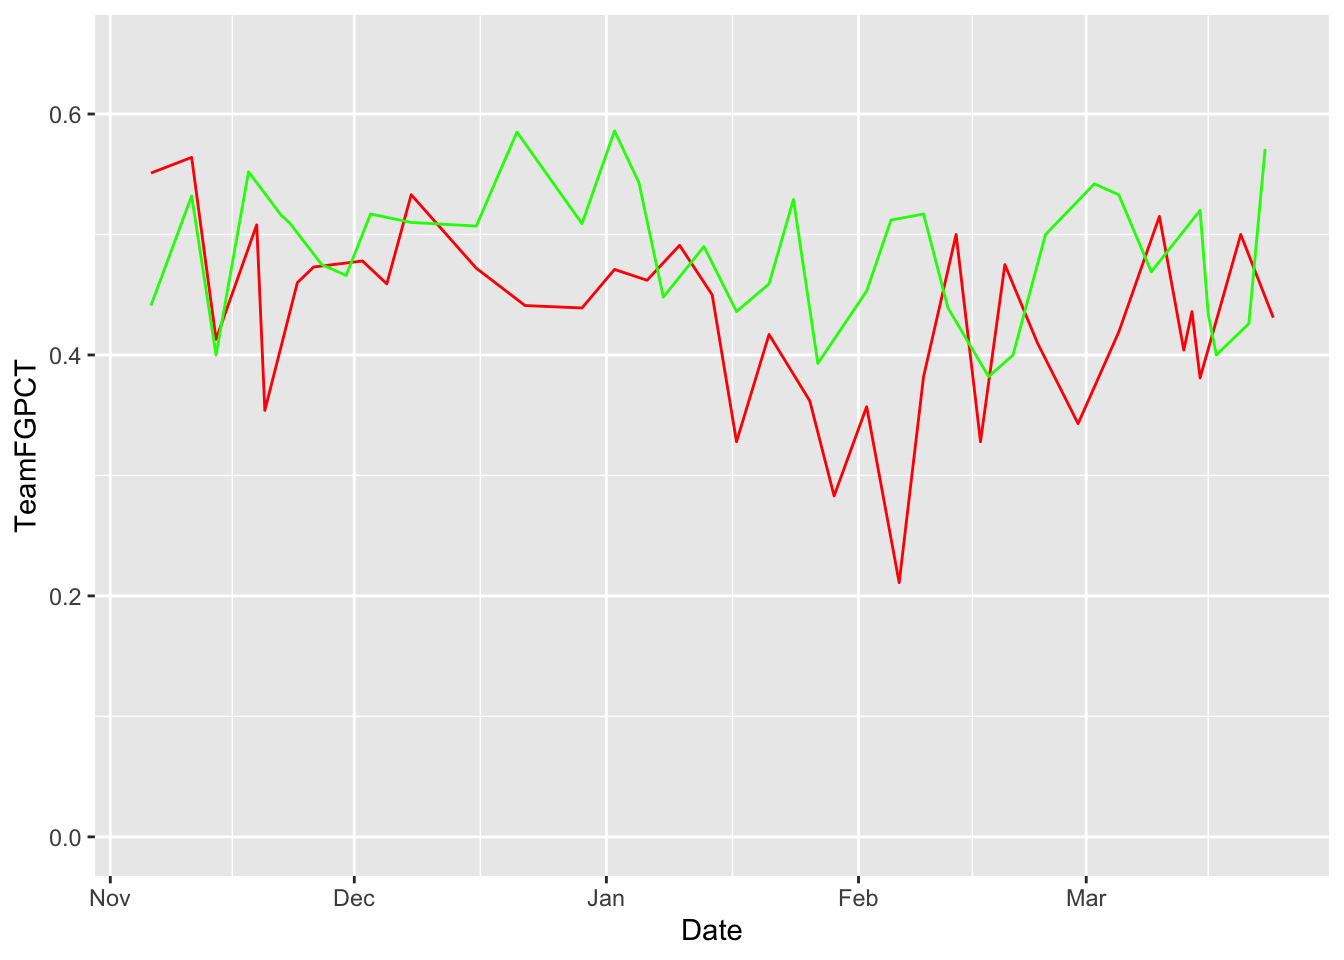
\includegraphics{datajournalism_files/figure-latex/unnamed-chunk-151-1.pdf}

Better, but it looks \ldots{} not great on the bottom. We can fix that by flipping the coordinates.

\begin{Shaded}
\begin{Highlighting}[]
\KeywordTok{ggplot}\NormalTok{() }\OperatorTok{+}\StringTok{ }\KeywordTok{geom_bar}\NormalTok{(}\DataTypeTok{data=}\NormalTok{topsightings, }\KeywordTok{aes}\NormalTok{(}\DataTypeTok{x=}\KeywordTok{reorder}\NormalTok{(COUNTY, total), }\DataTypeTok{weight=}\NormalTok{total)) }\OperatorTok{+}\StringTok{ }\KeywordTok{coord_flip}\NormalTok{()}
\end{Highlighting}
\end{Shaded}

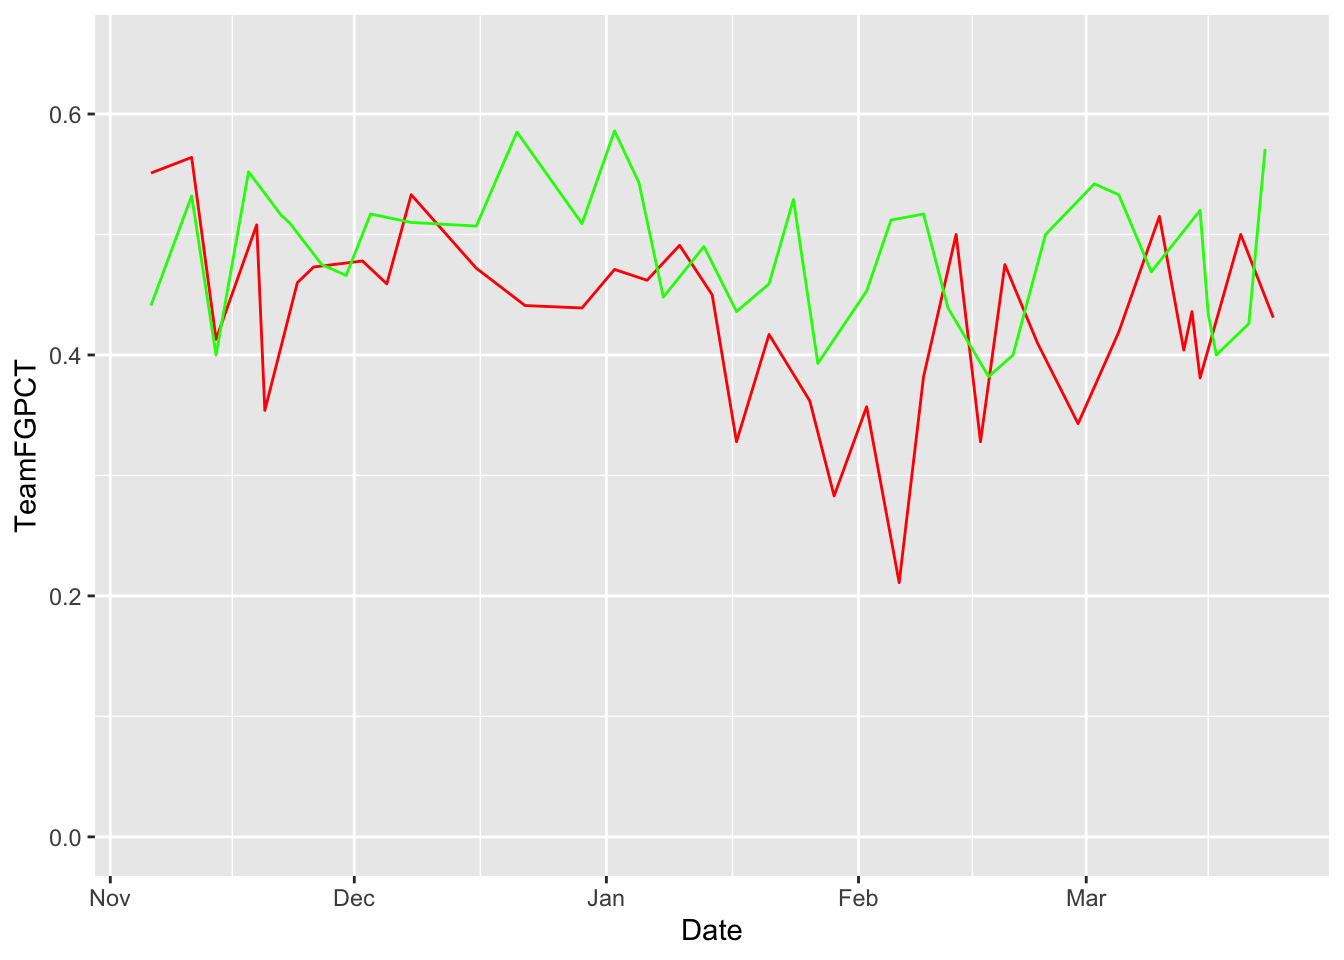
\includegraphics{datajournalism_files/figure-latex/unnamed-chunk-152-1.pdf}

Art? No.~Tells you the story? Yep. And for reporting purposes, that's enough.

\hypertarget{line-charts}{%
\section{Line charts}\label{line-charts}}

Line charts show change over time. It works the much the same as a bar chart, code wise, but instead of a weight, it uses a y. And if you have more than one group in your data, it takes a group element.

The secret to knowing if you have a line chart is if you have a date. The secret to making a line chart is your x value is almost always a date.

To make this easier, I've created a new version of the \href{https://unl.box.com/s/v4d3uyteuzhxqjl3nfn9f5lhe16a2fq4}{county population estimates data that it formatted for charting}. Let's import it:

\begin{Shaded}
\begin{Highlighting}[]
\NormalTok{populationestimates <-}\StringTok{ }\KeywordTok{read_csv}\NormalTok{(}\StringTok{"data/countypopulationslong.csv"}\NormalTok{)}
\end{Highlighting}
\end{Shaded}

\begin{verbatim}
## Parsed with column specification:
## cols(
##   STNAME = col_character(),
##   CTYNAME = col_character(),
##   Year = col_character(),
##   Population = col_double(),
##   Date = col_date(format = ""),
##   Name = col_character()
## )
\end{verbatim}

As you can see, I've switched the data from the years going wide to the right to each line being one county, one year. And, I've added a date column, which is the estimates date.

Now, if we tried to make a line chart of all 3,142 counties, we'd get a mess. But, it's the first mistake people make in creating a line chart, so let's do that.

\begin{Shaded}
\begin{Highlighting}[]
\KeywordTok{ggplot}\NormalTok{() }\OperatorTok{+}\StringTok{ }\KeywordTok{geom_line}\NormalTok{(}\DataTypeTok{data=}\NormalTok{populationestimates, }\KeywordTok{aes}\NormalTok{(}\DataTypeTok{x=}\NormalTok{Date, }\DataTypeTok{y=}\NormalTok{Population, }\DataTypeTok{group=}\NormalTok{Name))}
\end{Highlighting}
\end{Shaded}

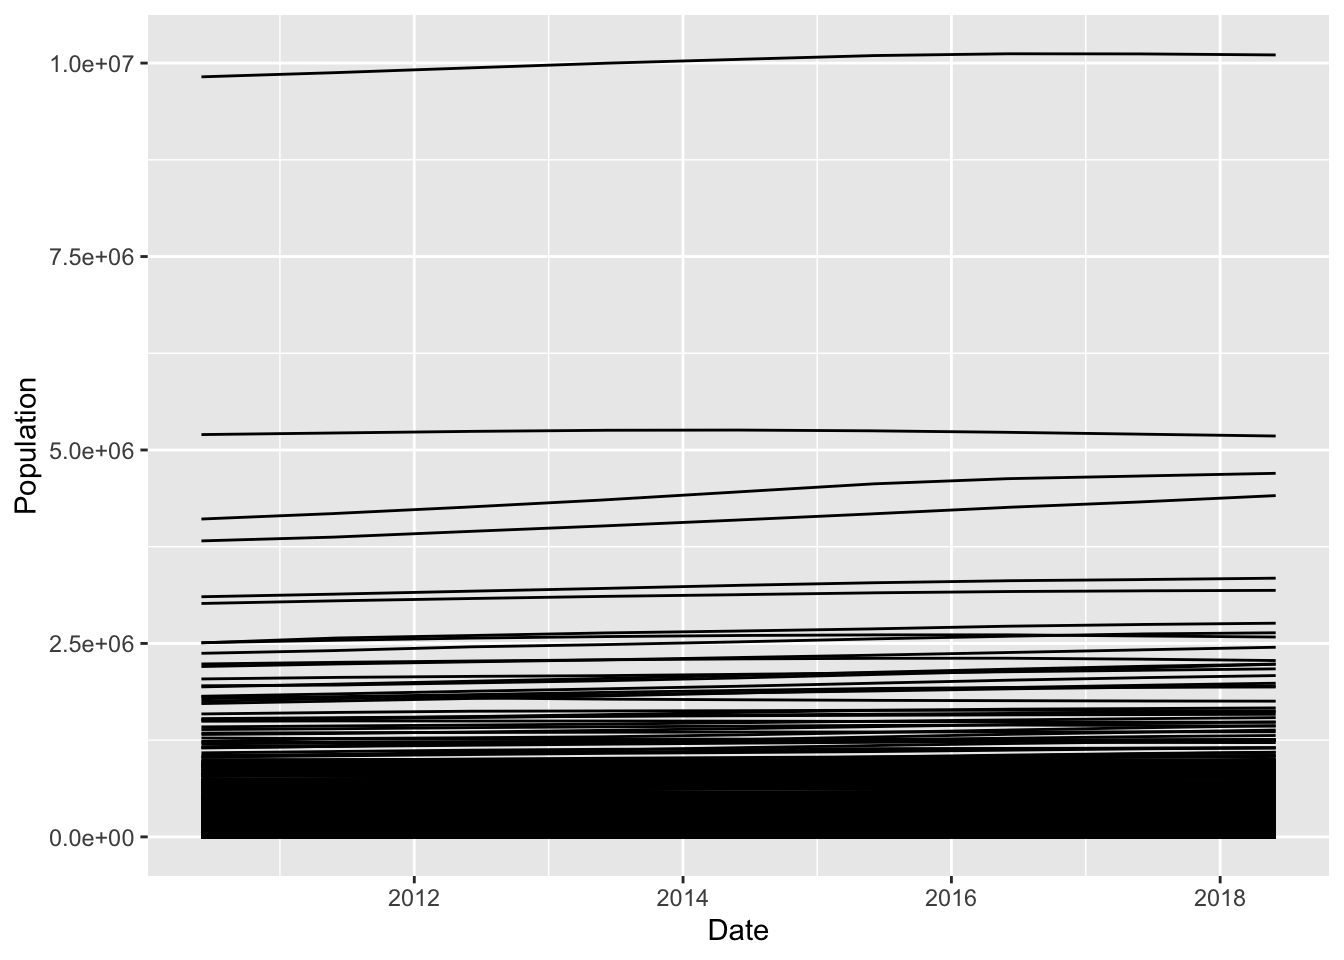
\includegraphics{datajournalism_files/figure-latex/unnamed-chunk-154-1.pdf}

And what do we learn from this? There's one very, very big county, some less big counties, and a ton of smaller counties. So many we can't see Them, and because the numbers are so big, any changes are dwarfed.

So let's thin the herd here. How about we just look at Lancaster County, Nebraska.

\begin{Shaded}
\begin{Highlighting}[]
\NormalTok{lancaster <-}\StringTok{ }\NormalTok{populationestimates }\OperatorTok\StringTok{ }\KeywordTok{filter}\NormalTok{(Name }\OperatorTok{==}\StringTok{ "Lancaster County, Nebraska"}\NormalTok{)}
\end{Highlighting}
\end{Shaded}

Now let's chart it.

\begin{Shaded}
\begin{Highlighting}[]
\KeywordTok{ggplot}\NormalTok{() }\OperatorTok{+}\StringTok{ }\KeywordTok{geom_line}\NormalTok{(}\DataTypeTok{data=}\NormalTok{lancaster, }\KeywordTok{aes}\NormalTok{(}\DataTypeTok{x=}\NormalTok{Date, }\DataTypeTok{y=}\NormalTok{Population, }\DataTypeTok{group=}\NormalTok{Name))}
\end{Highlighting}
\end{Shaded}

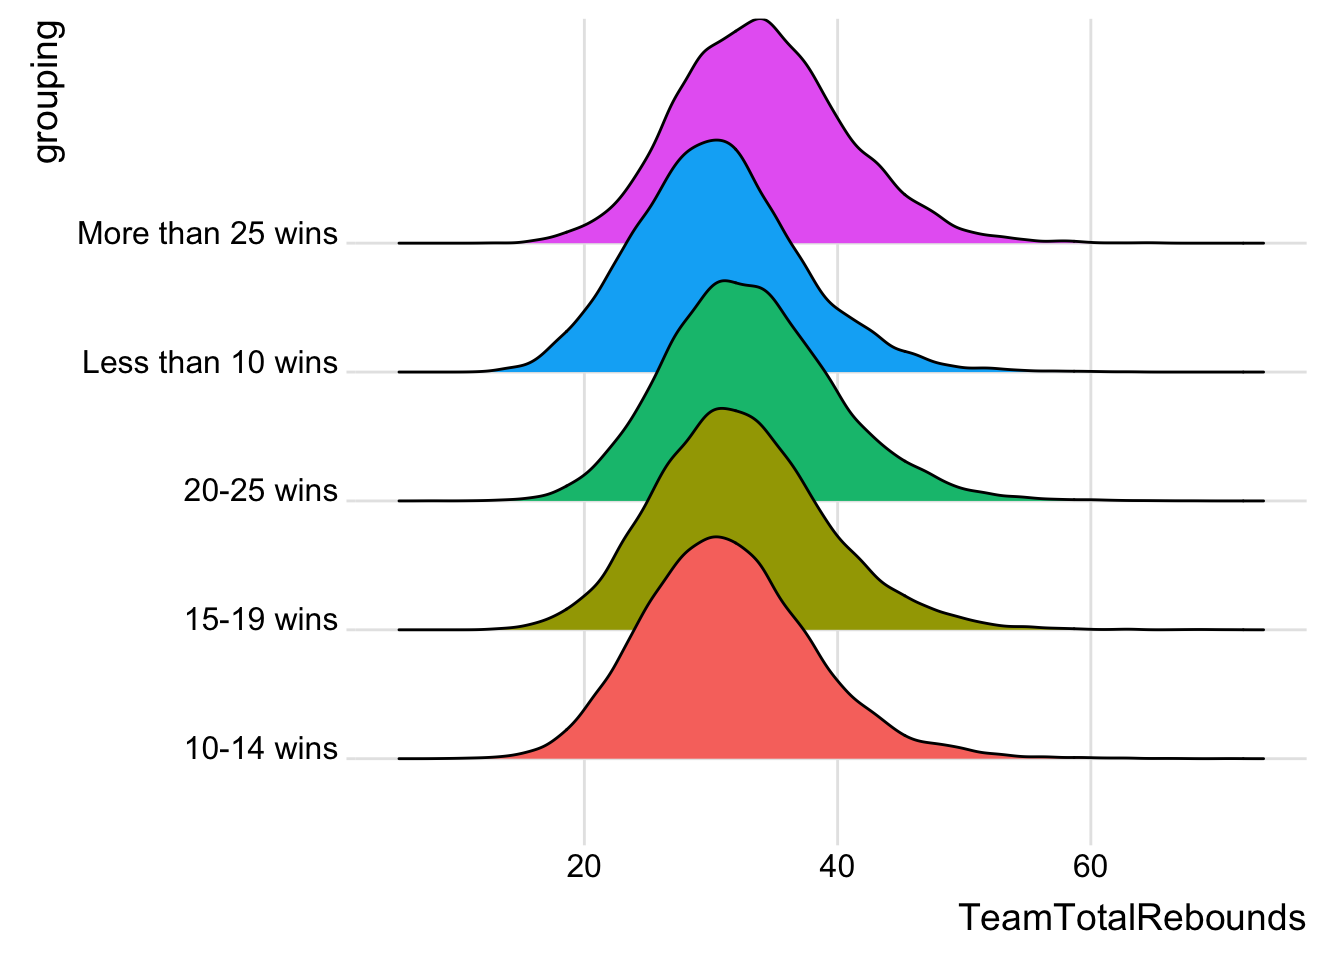
\includegraphics{datajournalism_files/figure-latex/unnamed-chunk-156-1.pdf}

Growing like gangbusters, right? Well, not exactly. Note the y axis doesn't start at 0.

\begin{Shaded}
\begin{Highlighting}[]
\KeywordTok{ggplot}\NormalTok{() }\OperatorTok{+}\StringTok{ }\KeywordTok{geom_line}\NormalTok{(}\DataTypeTok{data=}\NormalTok{lancaster, }\KeywordTok{aes}\NormalTok{(}\DataTypeTok{x=}\NormalTok{Date, }\DataTypeTok{y=}\NormalTok{Population, }\DataTypeTok{group=}\NormalTok{Name)) }\OperatorTok{+}\StringTok{ }\KeywordTok{scale_y_continuous}\NormalTok{(}\DataTypeTok{limits =} \KeywordTok{c}\NormalTok{(}\DecValTok{0}\NormalTok{, }\DecValTok{320000}\NormalTok{))}
\end{Highlighting}
\end{Shaded}

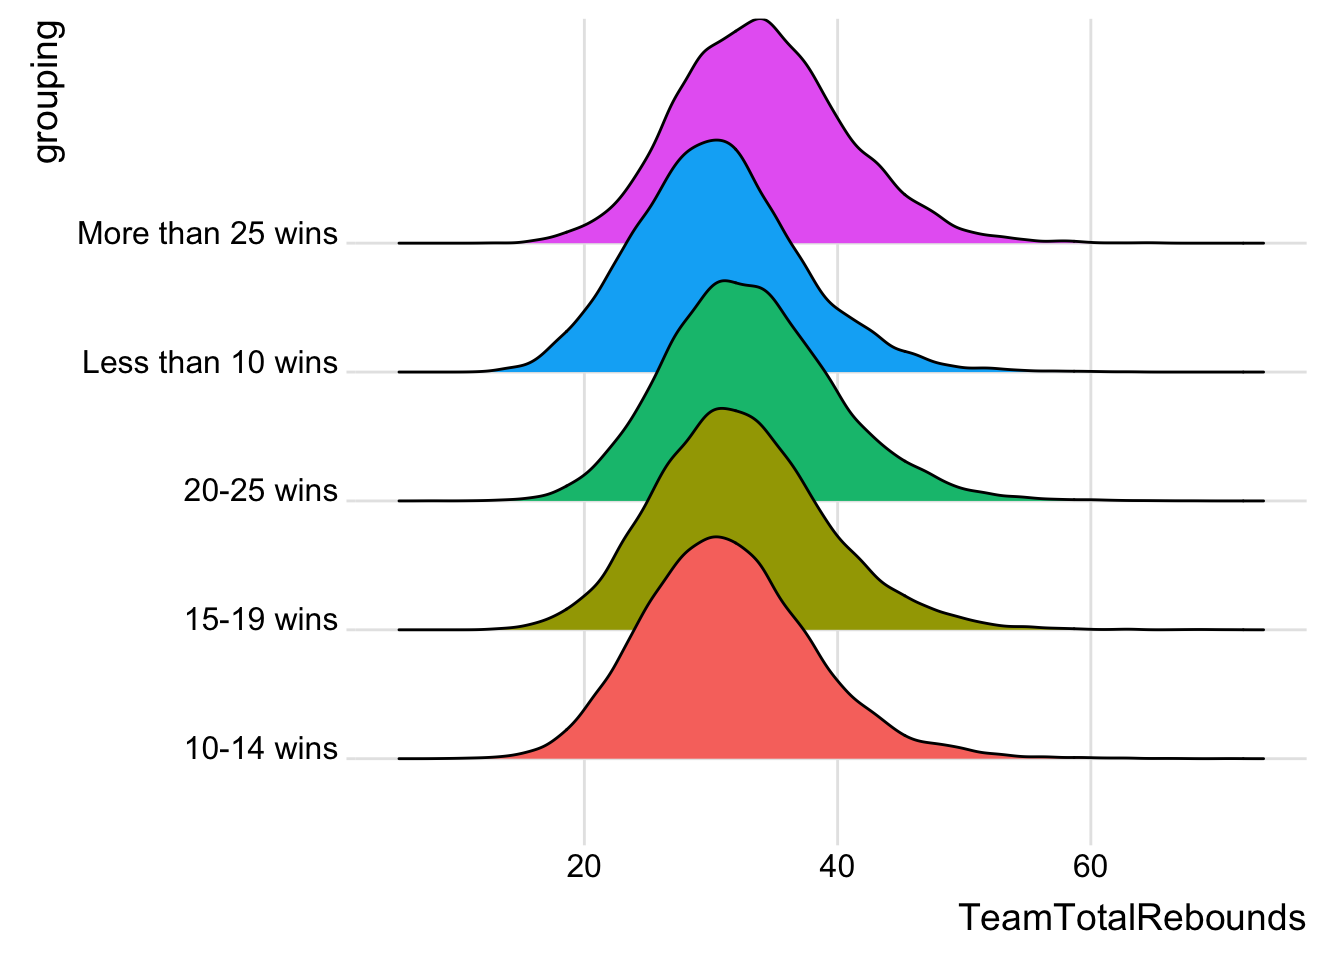
\includegraphics{datajournalism_files/figure-latex/unnamed-chunk-157-1.pdf}

More accurate.

But how does that compare to Omaha? Geoms work in layers. We can just add Omaha. First, we need a dataframe with Douglas County in it.

\begin{Shaded}
\begin{Highlighting}[]
\NormalTok{douglas <-}\StringTok{ }\NormalTok{populationestimates }\OperatorTok\StringTok{ }\KeywordTok{filter}\NormalTok{(Name }\OperatorTok{==}\StringTok{ "Douglas County, Nebraska"}\NormalTok{)}
\end{Highlighting}
\end{Shaded}

With that, we just add another geom\_line. We will also need to adjust our y axis limits to expand to fit Omaha.

\begin{Shaded}
\begin{Highlighting}[]
\KeywordTok{ggplot}\NormalTok{() }\OperatorTok{+}\StringTok{ }\KeywordTok{geom_line}\NormalTok{(}\DataTypeTok{data=}\NormalTok{lancaster, }\KeywordTok{aes}\NormalTok{(}\DataTypeTok{x=}\NormalTok{Date, }\DataTypeTok{y=}\NormalTok{Population, }\DataTypeTok{group=}\NormalTok{Name)) }\OperatorTok{+}\StringTok{ }\KeywordTok{geom_line}\NormalTok{(}\DataTypeTok{data=}\NormalTok{douglas, }\KeywordTok{aes}\NormalTok{(}\DataTypeTok{x=}\NormalTok{Date, }\DataTypeTok{y=}\NormalTok{Population, }\DataTypeTok{group=}\NormalTok{Name)) }\OperatorTok{+}\StringTok{ }\KeywordTok{scale_y_continuous}\NormalTok{(}\DataTypeTok{limits =} \KeywordTok{c}\NormalTok{(}\DecValTok{0}\NormalTok{, }\DecValTok{650000}\NormalTok{))}
\end{Highlighting}
\end{Shaded}

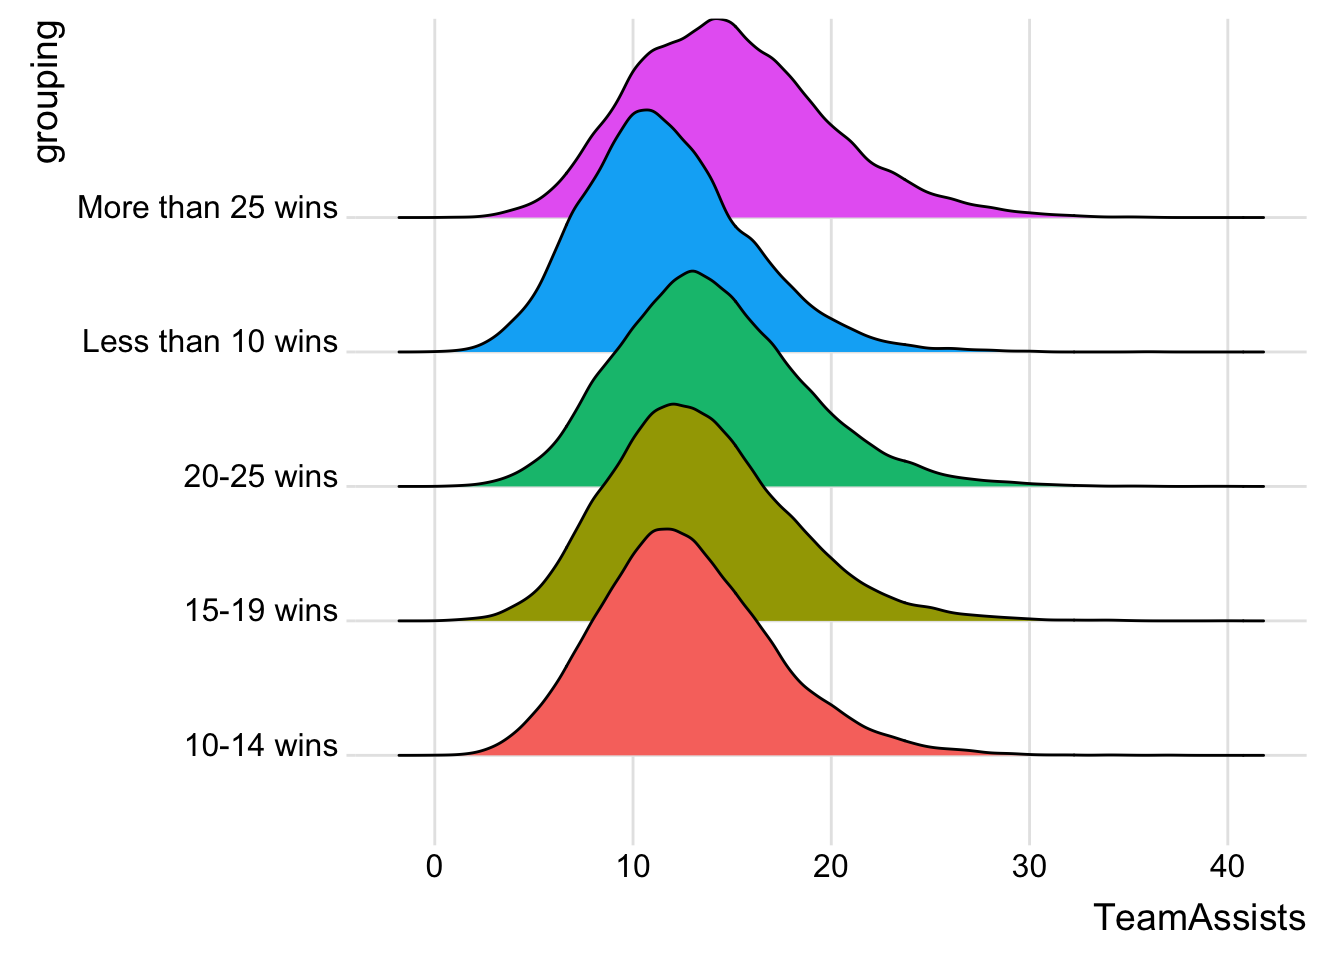
\includegraphics{datajournalism_files/figure-latex/unnamed-chunk-159-1.pdf}

So both counties are growing, but from the line we can see that Omaha is growing just ever so slightly faster. No accounting for taste.

\hypertarget{visualizing-your-data-for-publication}{%
\chapter{Visualizing your data for publication}\label{visualizing-your-data-for-publication}}

Doing data visualization well, and at professional level, takes time, skill and practice to perfect. Understanding it and doing it at a complex level is an entire class on it's own. It uses some of the same skills here -- grouping, filtering, calculating -- but then takes that data and turns it into data pictures.

But simple stuff -- and even some slightly complicated stuff -- can be done with tools made for people who aren't data viz pros.

The tool we're going to use is called \href{https://www.datawrapper.de/}{Datawrapper}.

First, let's get some data and work with it. \href{https://ourworldindata.org/coronavirus-source-data}{The WHO is publishing corona data as a CSV daily}. Let's look at it.

\begin{Shaded}
\begin{Highlighting}[]
\KeywordTok{library}\NormalTok{(tidyverse)}
\end{Highlighting}
\end{Shaded}

\begin{Shaded}
\begin{Highlighting}[]
\NormalTok{coronavirus <-}\StringTok{ }\KeywordTok{read_csv}\NormalTok{(}\StringTok{"https://covid.ourworldindata.org/data/full_data.csv"}\NormalTok{)}
\end{Highlighting}
\end{Shaded}

\begin{verbatim}
## Parsed with column specification:
## cols(
##   date = col_date(format = ""),
##   location = col_character(),
##   new_cases = col_double(),
##   new_deaths = col_double(),
##   total_cases = col_double(),
##   total_deaths = col_double()
## )
\end{verbatim}

\begin{Shaded}
\begin{Highlighting}[]
\KeywordTok{head}\NormalTok{(coronavirus)}
\end{Highlighting}
\end{Shaded}

\begin{verbatim}
## # A tibble: 6 x 6
##   date       location    new_cases new_deaths total_cases total_deaths
##   <date>     <chr>           <dbl>      <dbl>       <dbl>        <dbl>
## 1 2020-02-25 Afghanistan        NA         NA           1           NA
## 2 2020-02-26 Afghanistan         0         NA           1           NA
## 3 2020-02-27 Afghanistan         0         NA           1           NA
## 4 2020-02-28 Afghanistan         0         NA           1           NA
## 5 2020-02-29 Afghanistan         0         NA           1           NA
## 6 2020-03-01 Afghanistan         0         NA           1           NA
\end{verbatim}

Let's make a CSV of data from the United States. We can do that quickly by adding \texttt{write\_csv} to the end of a filter query.

\begin{Shaded}
\begin{Highlighting}[]
\NormalTok{coronavirus }\OperatorTok\StringTok{ }\KeywordTok{filter}\NormalTok{(location }\OperatorTok{==}\StringTok{ "United States"}\NormalTok{) }\OperatorTok\StringTok{ }\KeywordTok{write_csv}\NormalTok{(}\StringTok{"uscorona.csv"}\NormalTok{)}
\end{Highlighting}
\end{Shaded}

\hypertarget{datawrapper}{%
\section{Datawrapper}\label{datawrapper}}

Making charts in Datawrapper is preposterously simple, which is the point. There are dozens of chart types, and dozens of options. To get from a csv to a chart to publication is very, very easy.

First, go to \href{https://www.datawrapper.de/}{datawrapper.de} and sign up for an account. It's free.

Once logged in, you'll click on New Chart.

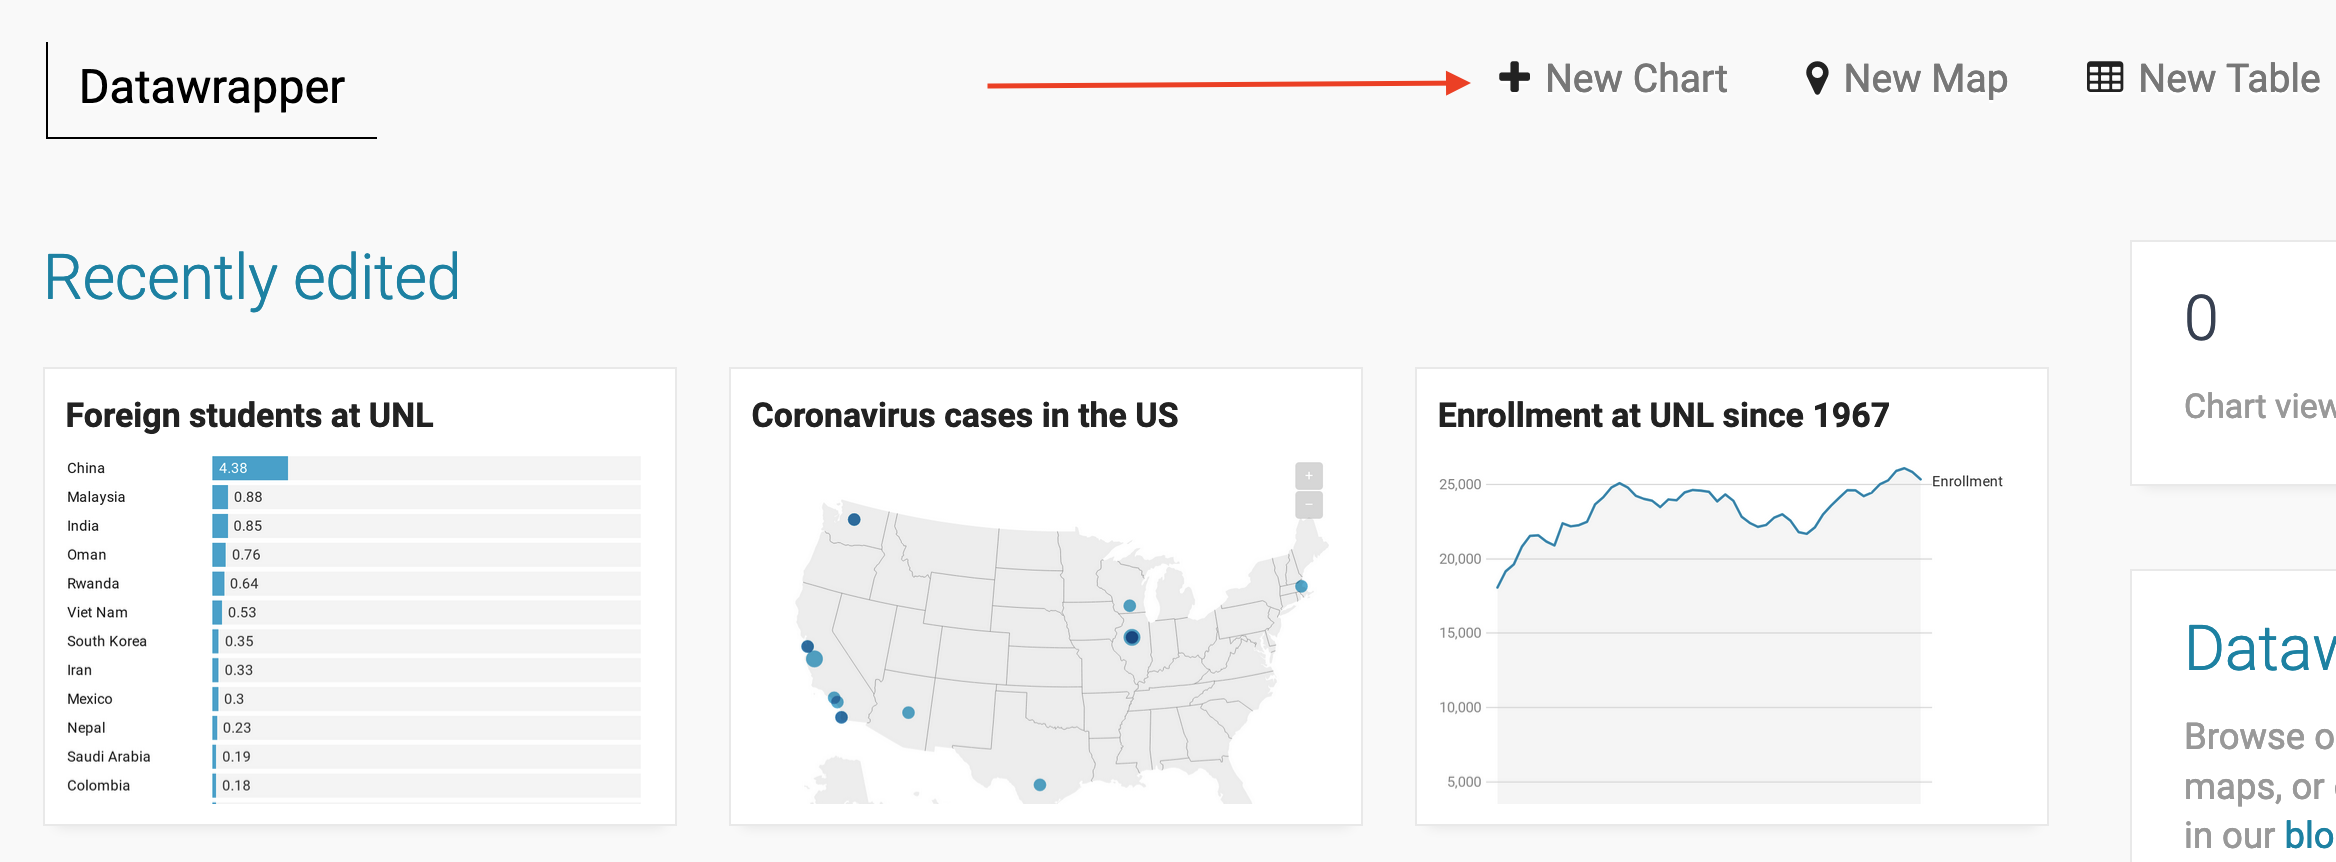
\includegraphics[width=32.44in]{images/datawrapper1}

The first thing we'll do is upload our CSV that we created before. Click on XLS/CSV and upload the file.

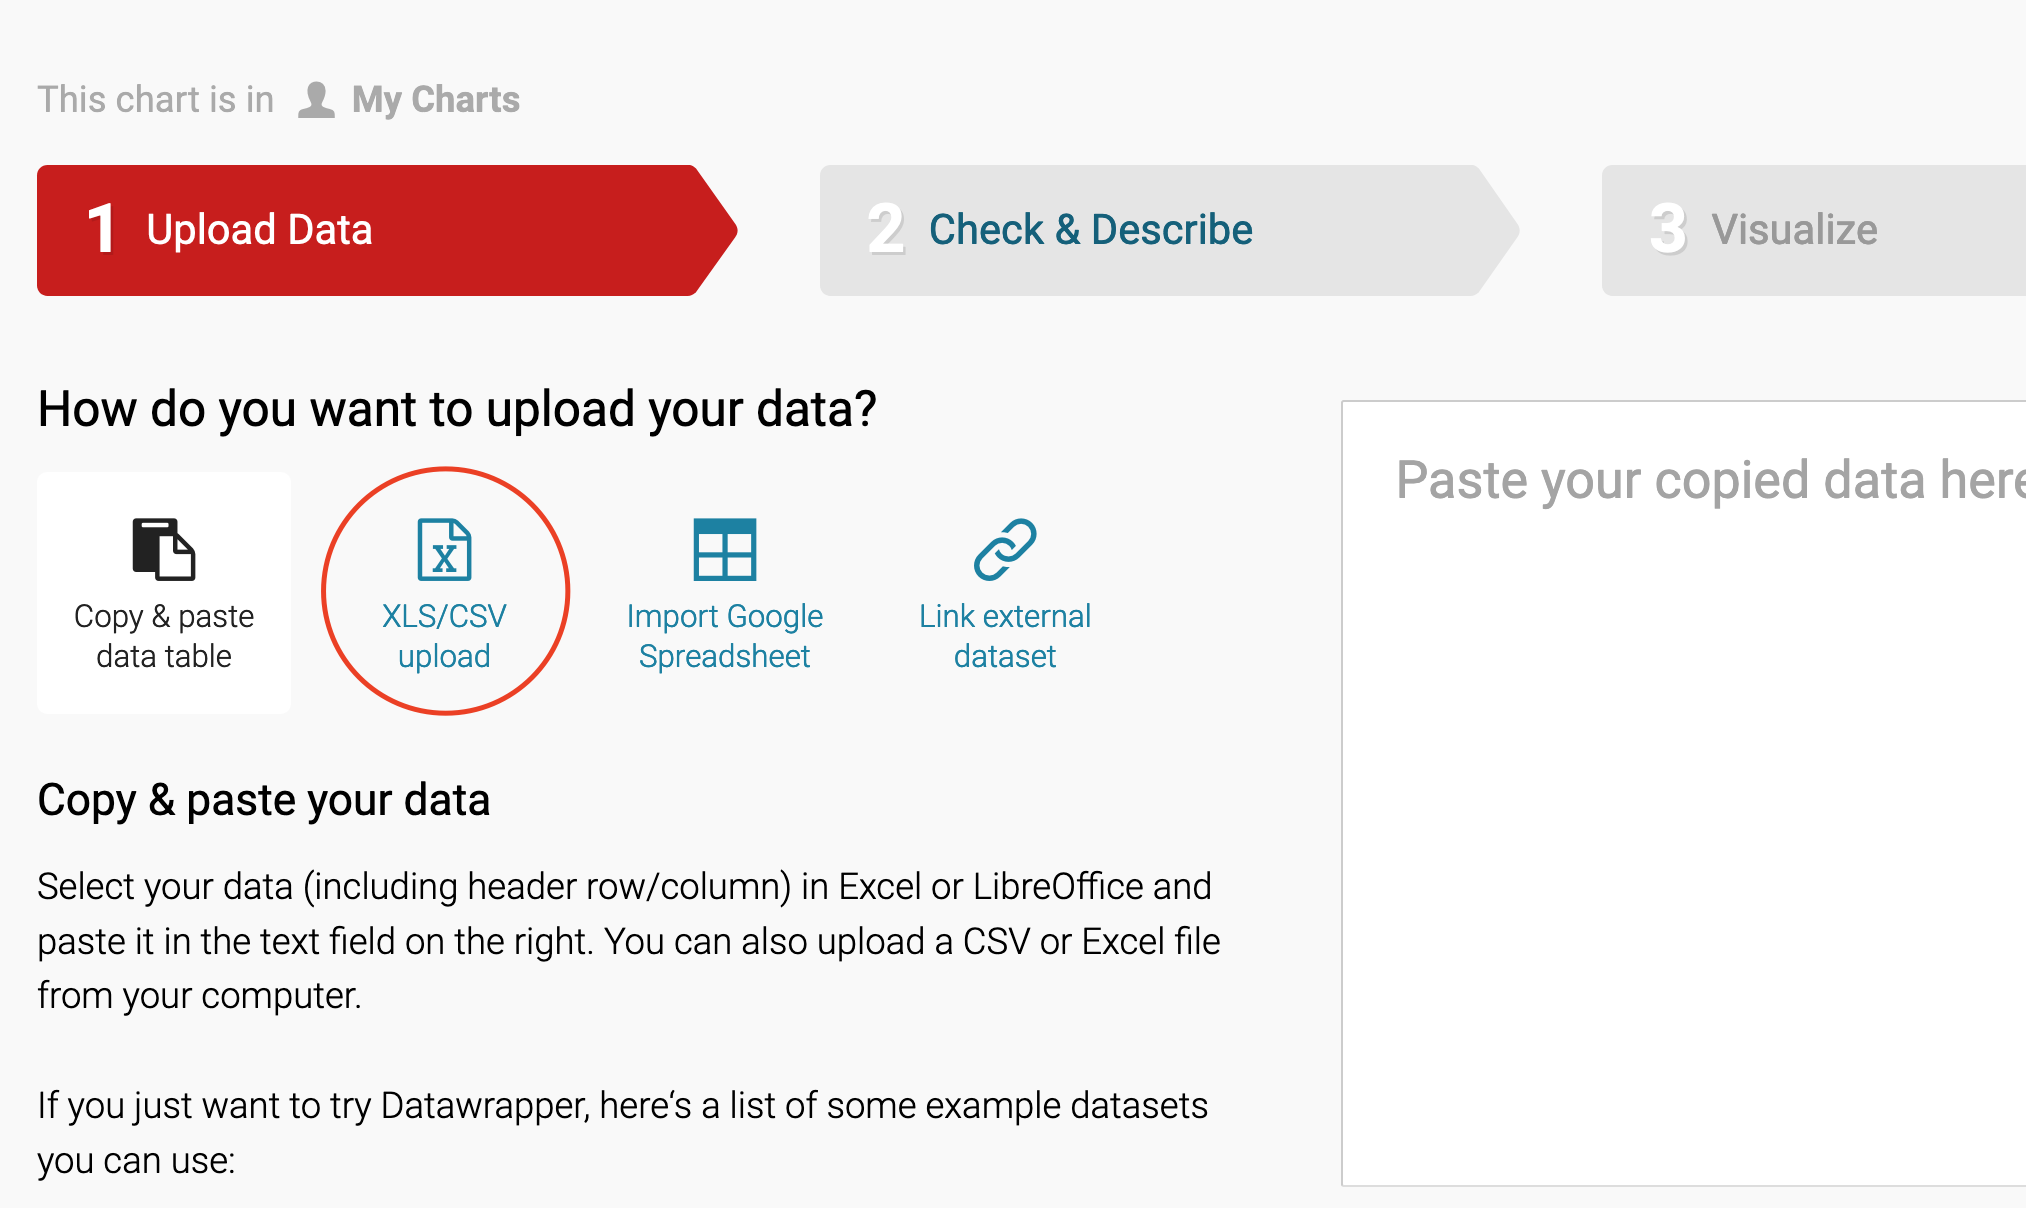
\includegraphics[width=28.14in]{images/datawrapper2}

Next up is to check and see what Datawrappper did with our data when we upoaded it. As you can see from the text on the left, if it's blue, it's a number. If it's green, it's a date. If it's black, it's text. Red means there's a problem. This data is very clean, so it imports cleanly.

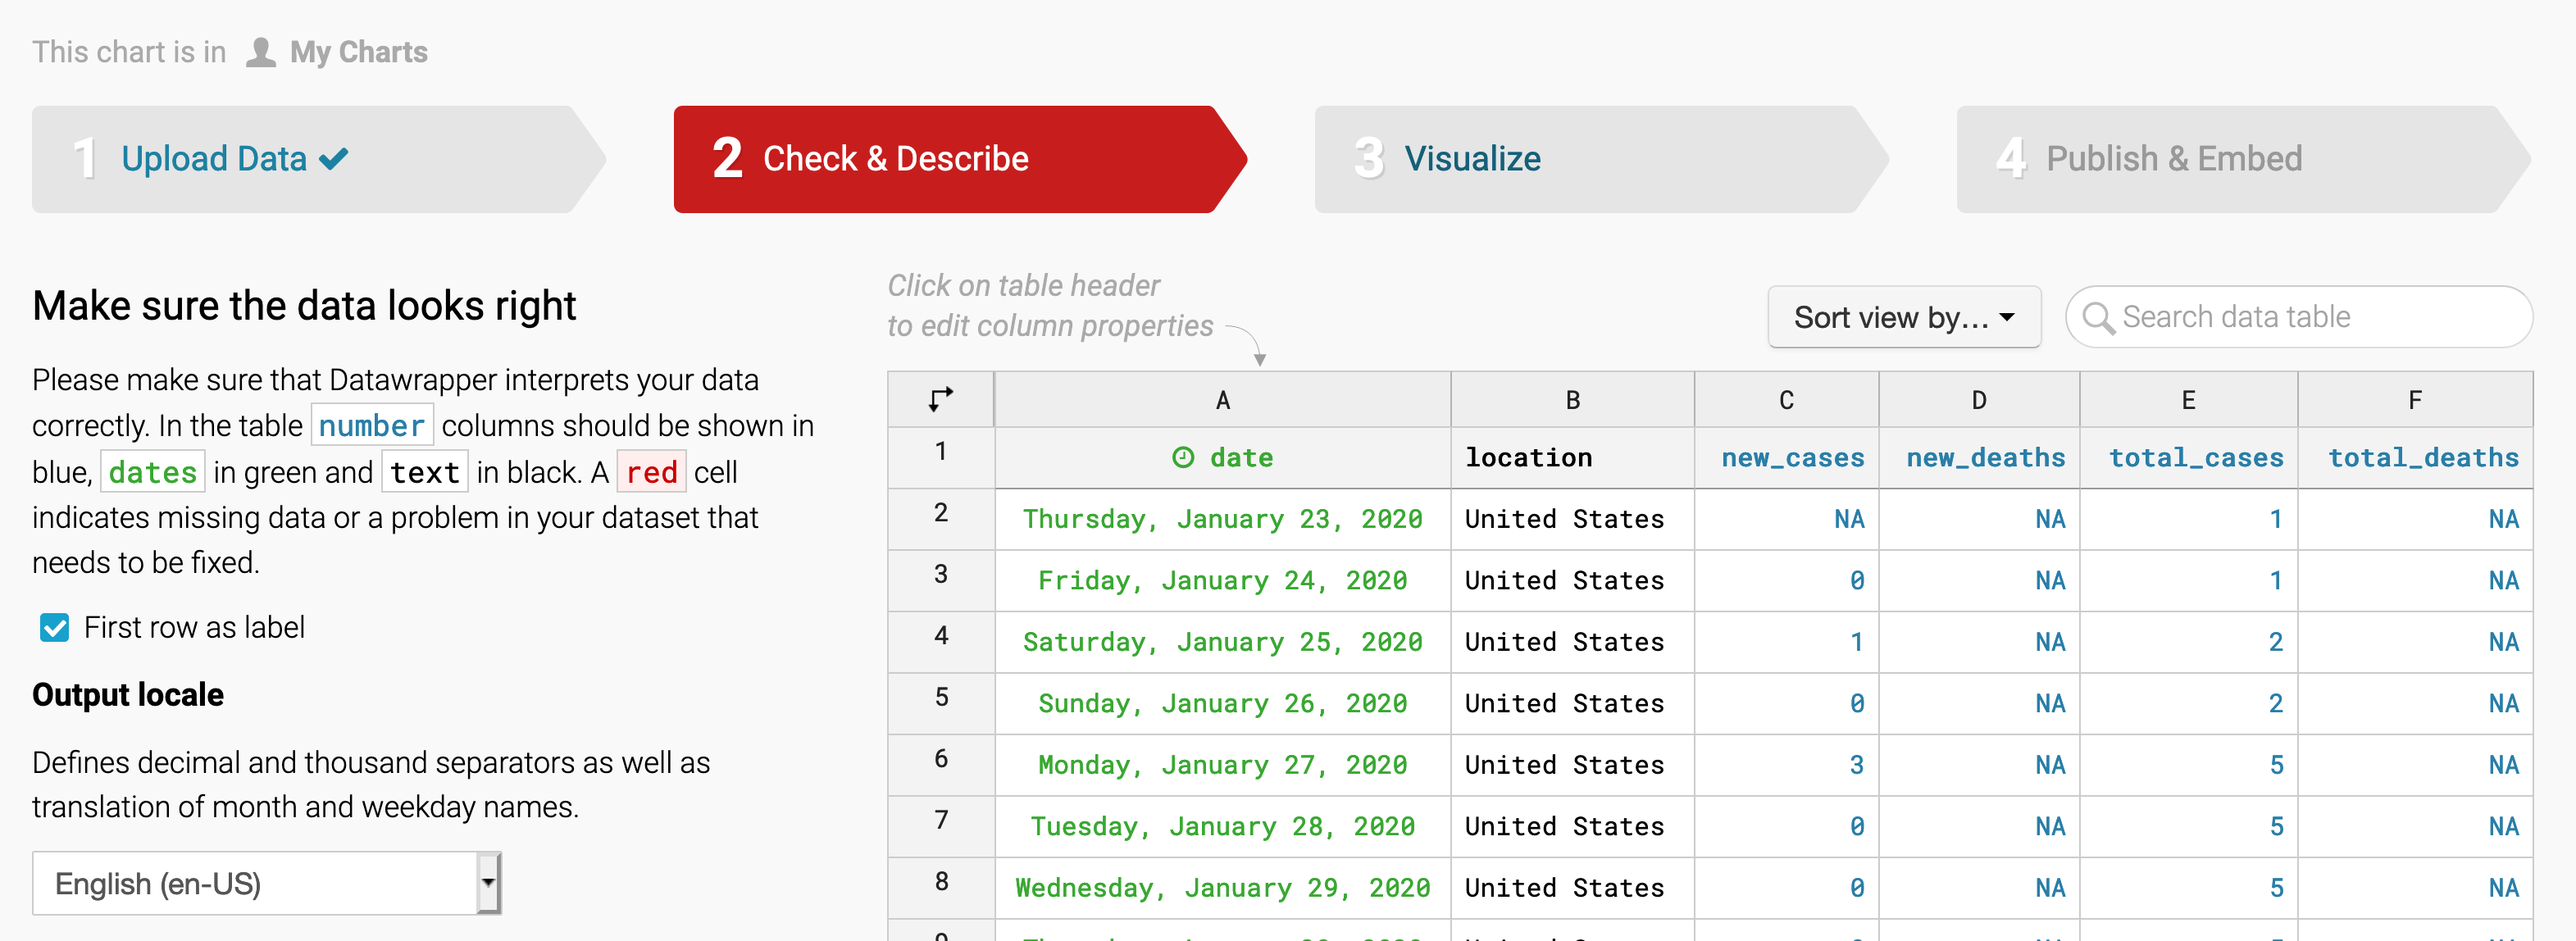
\includegraphics[width=43.64in]{images/datawrapper3}

Now we make a chart. Line chart comes up by default, which is good, because with date based data, that's what we have.

Click on Refine. The first option we want to change is the Tick format. Since we have only so many days of data, change it to months like below.

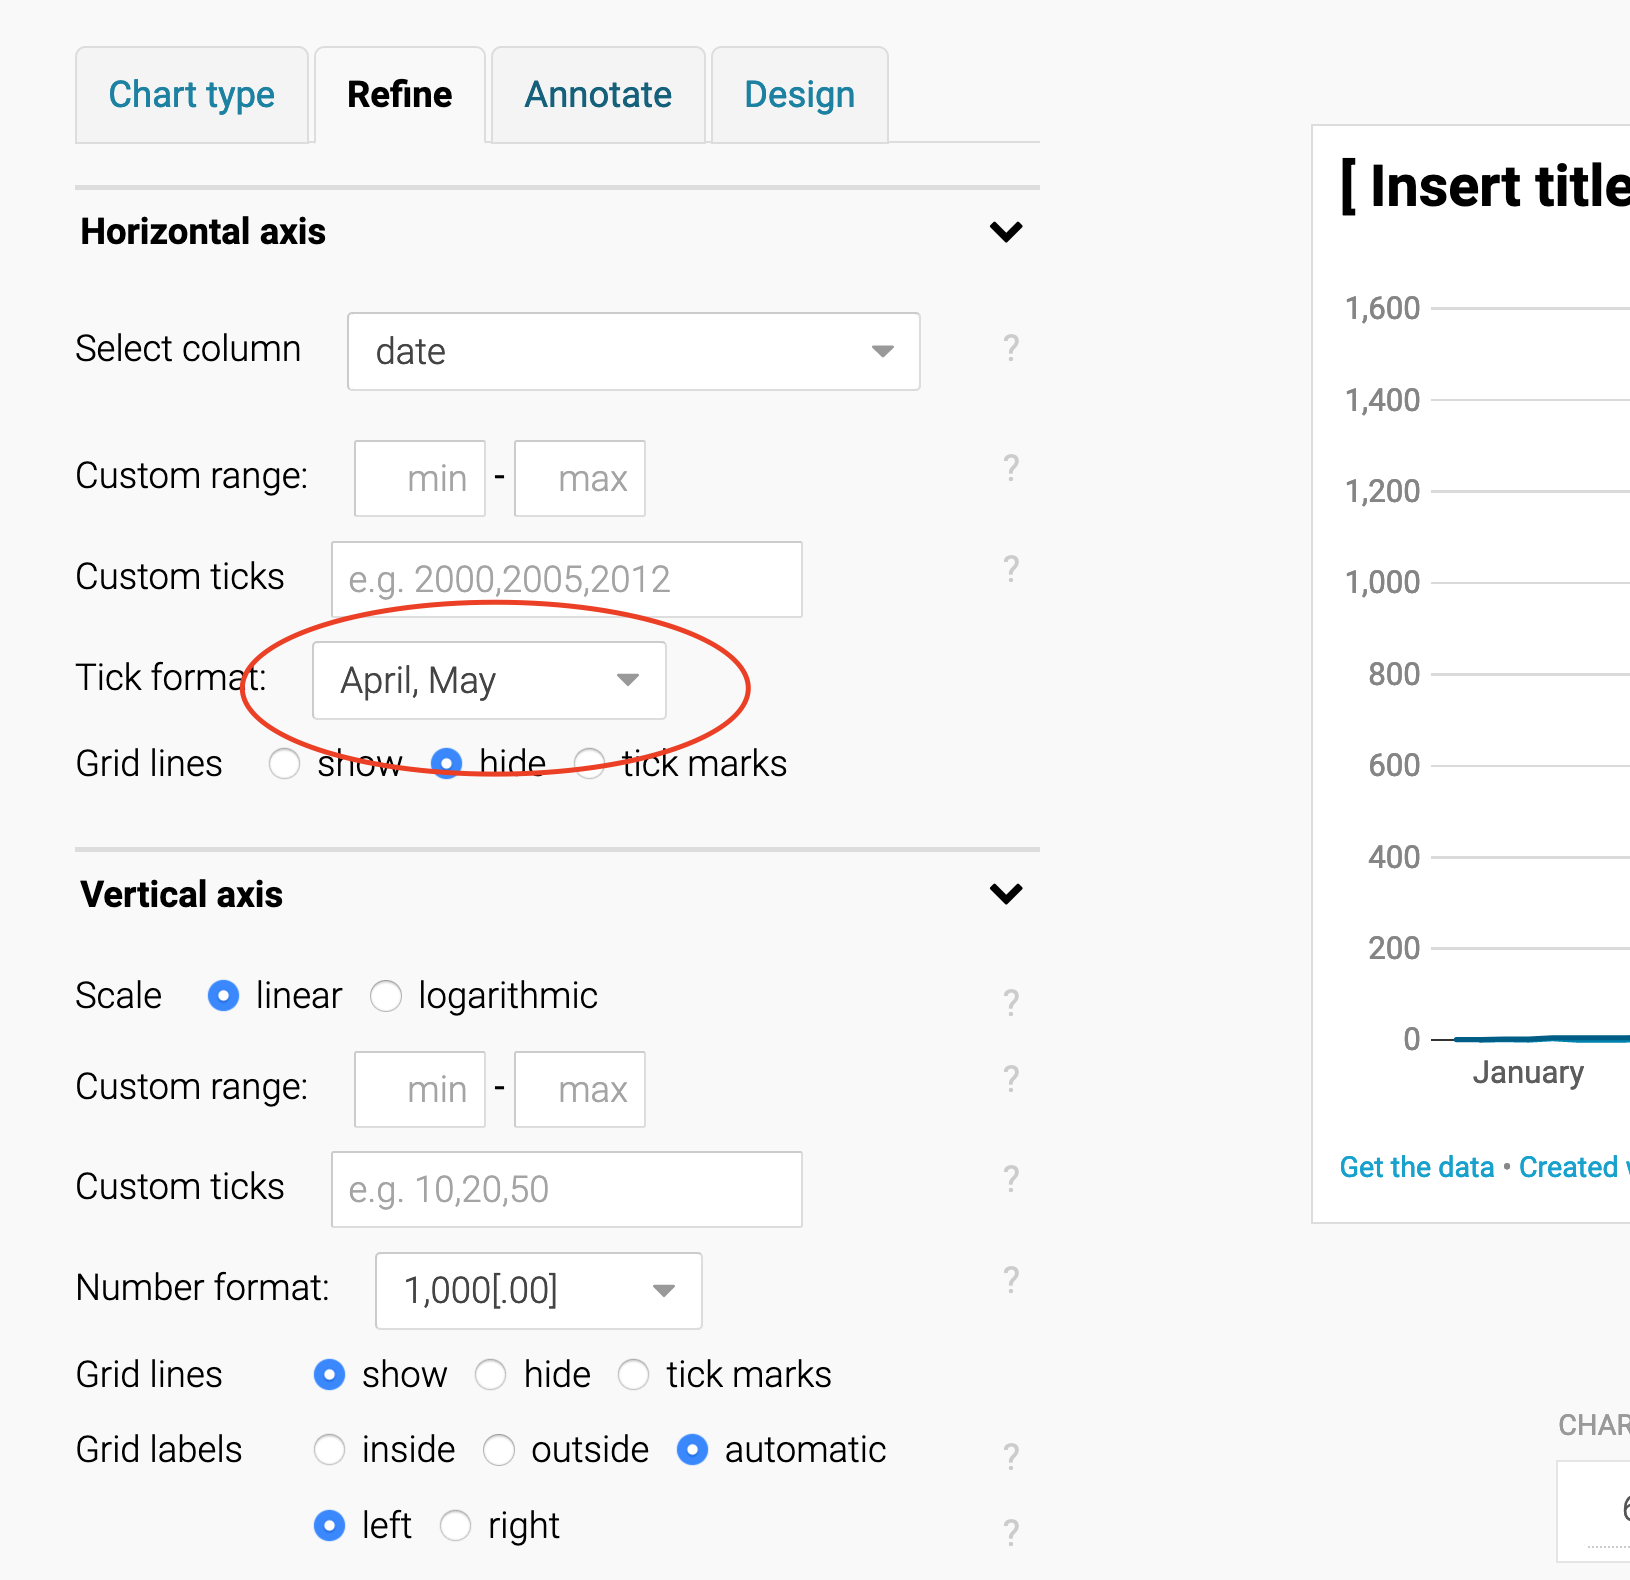
\includegraphics[width=22.64in]{images/datawrapper4}

Now we need to annotate our charts. Every chart needs a title, a source line and a credit line. Most need chatter (called description here).

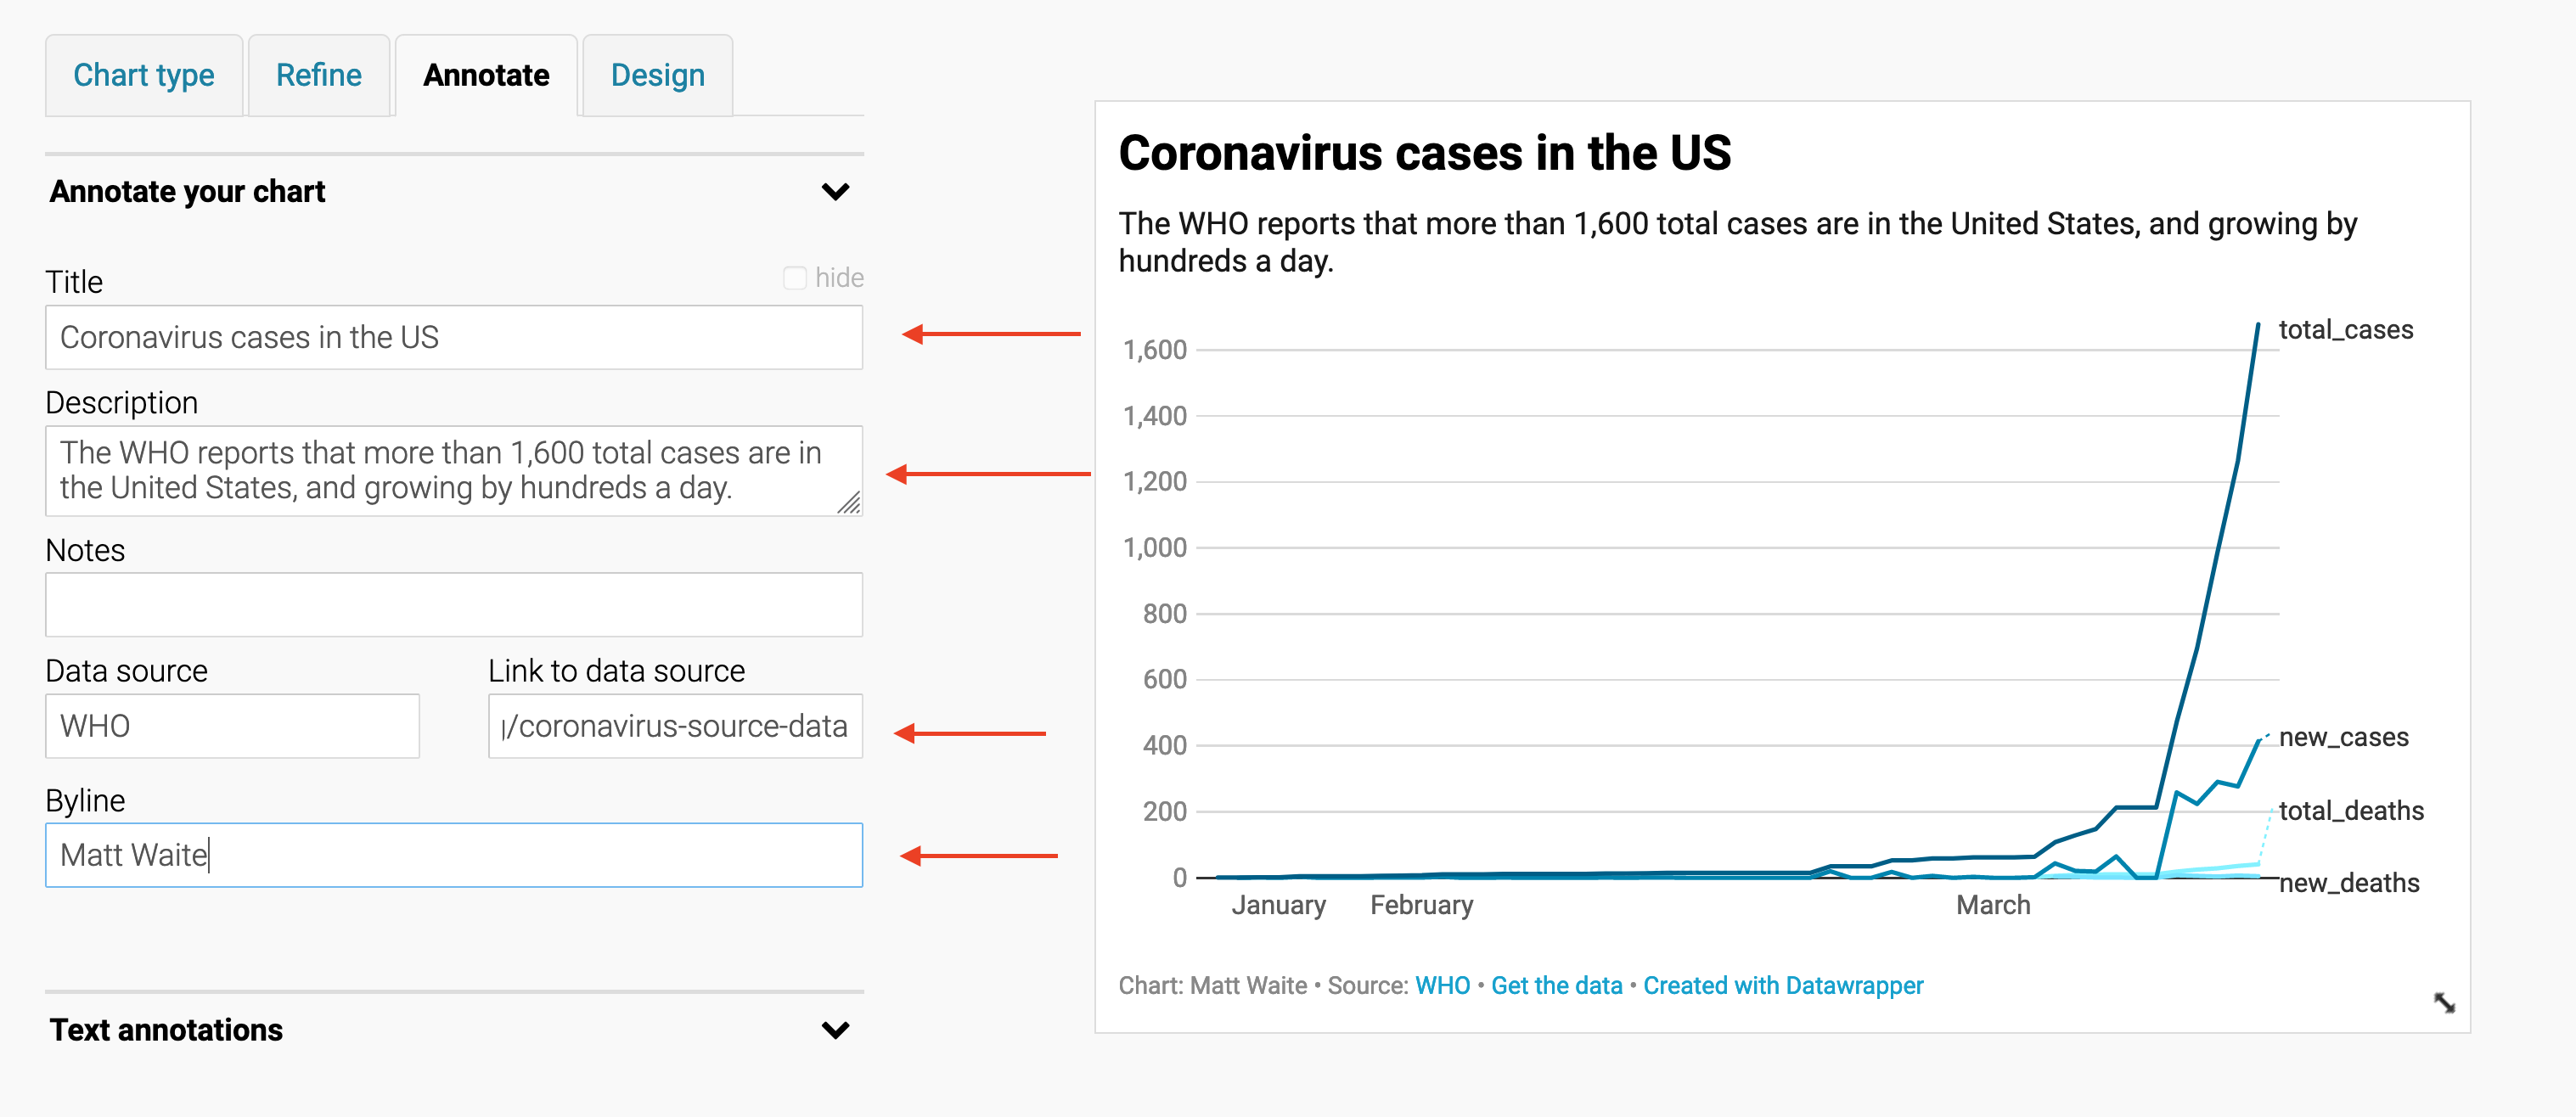
\includegraphics[width=42.14in]{images/datawrapper5}

The next thing is we can fix the labels at the ends of the line, to make them readable. Click on them, and a cursor should come up. Change them from the very data-y total\_cases to Total cases along with the rest.

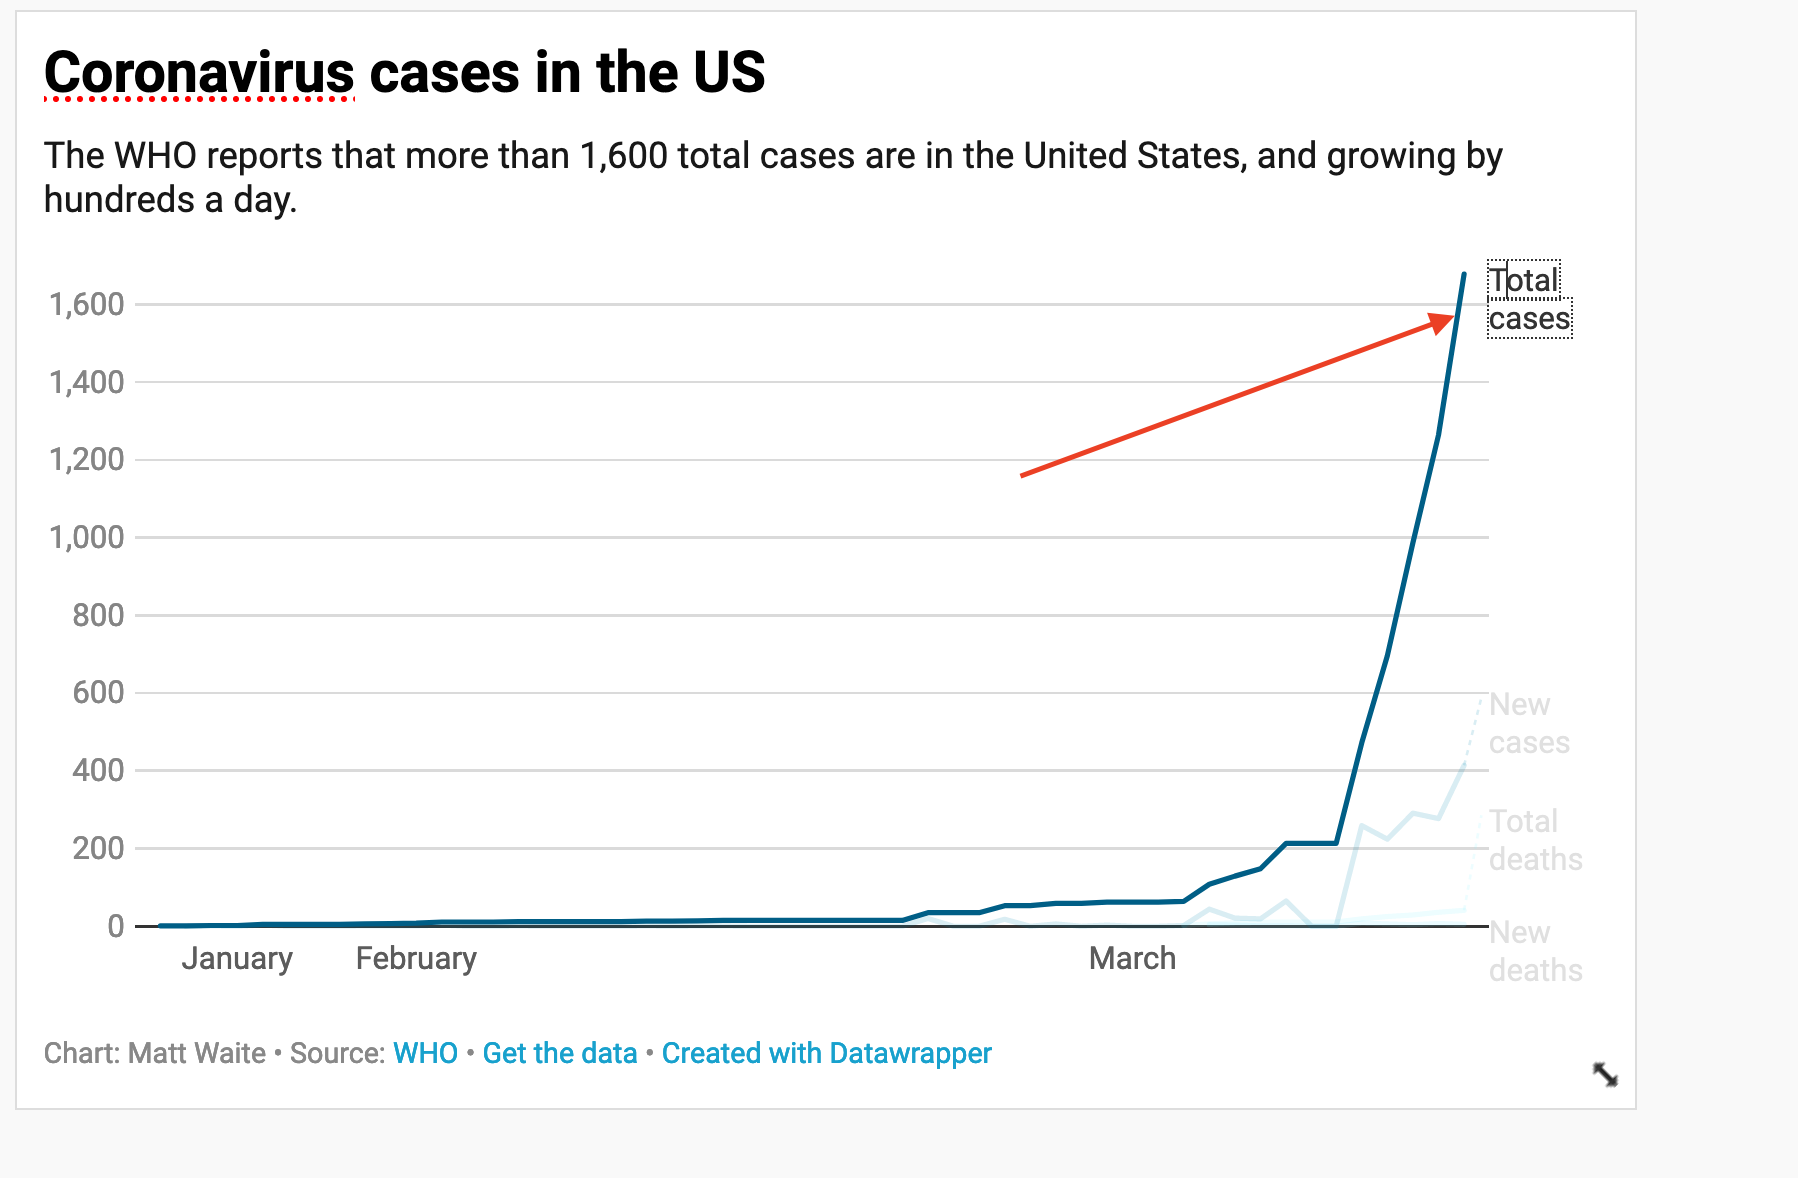
\includegraphics[width=24.97in]{images/datawrapper6}

Now we publish. Some publication systems allow for the embedding of HTML into a post or a story. Some don't. The only way to know is to ask someone at your publication. Every publication system on the planet, though, can publish an image. So there's always a way to export your chart as a PNG file, which you can upload like any photo.

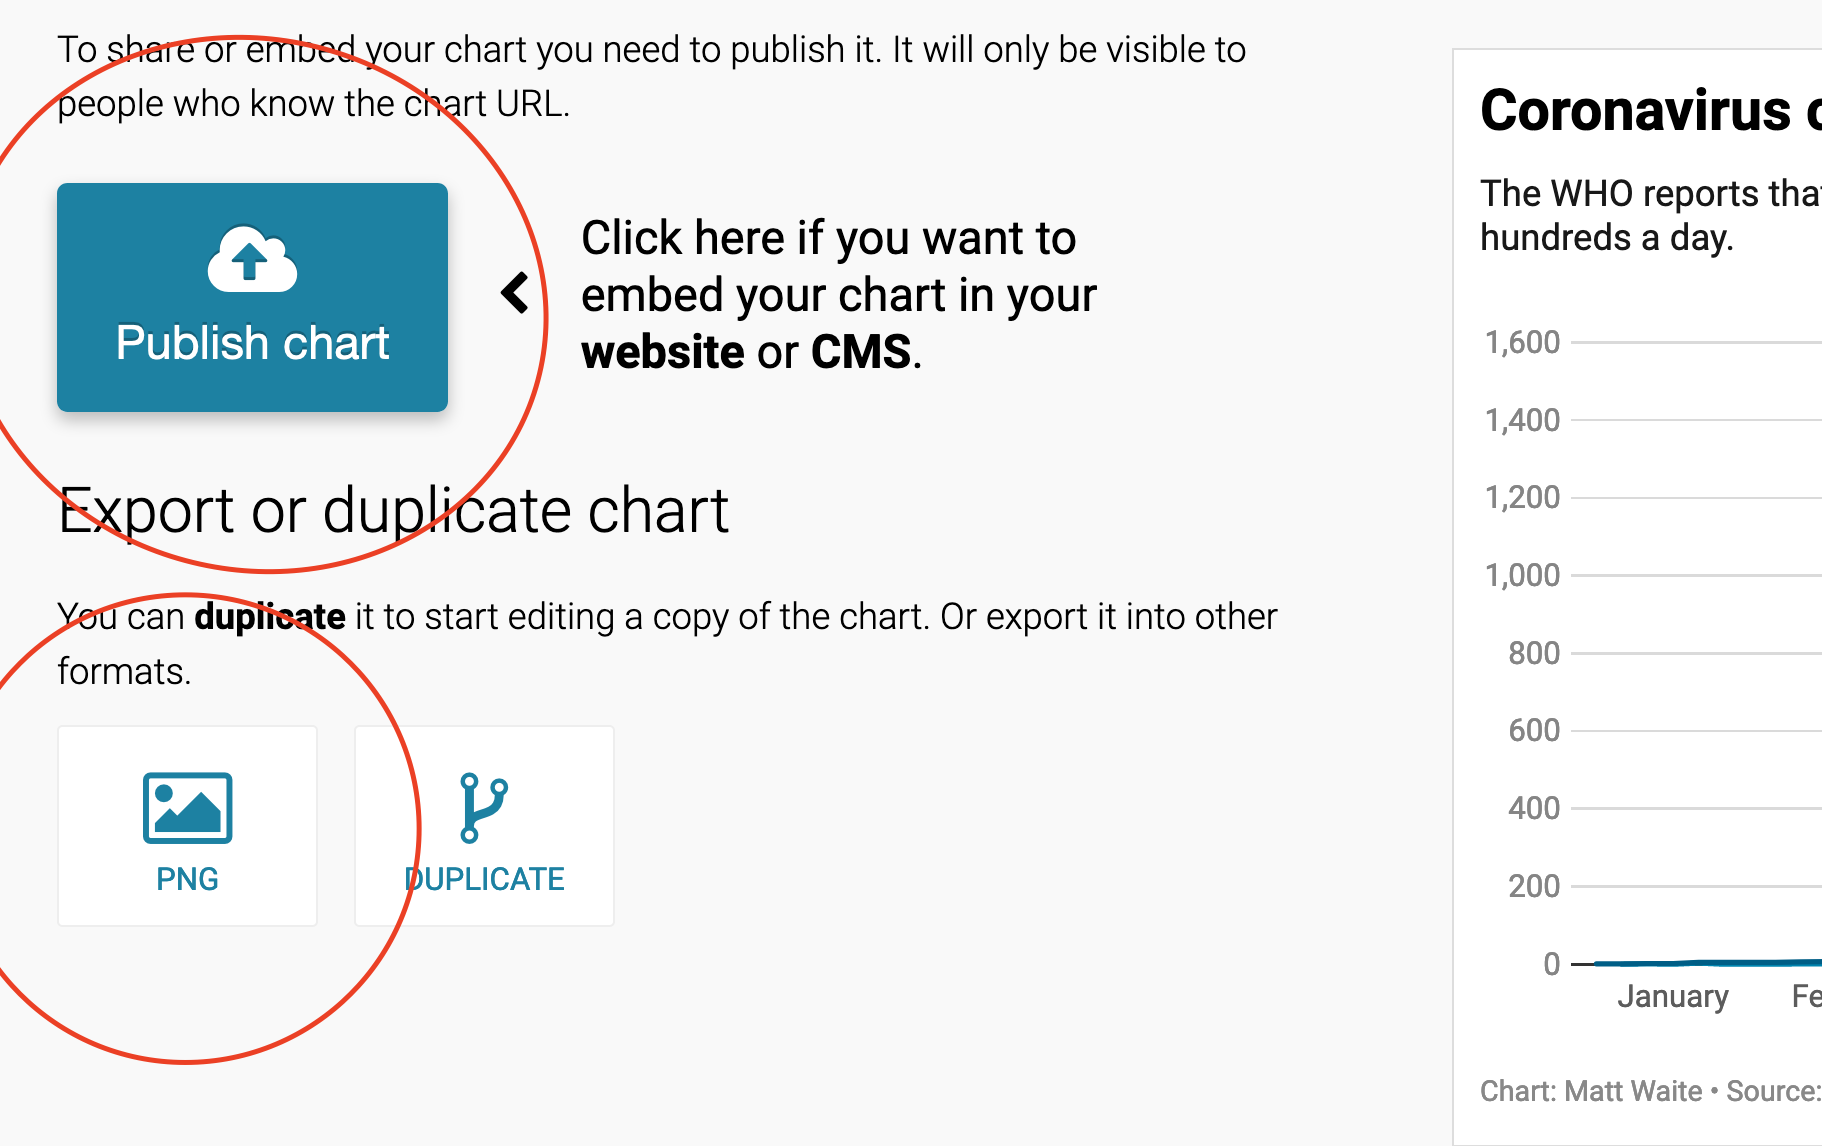
\includegraphics[width=25.31in]{images/datawrapper7}

\hypertarget{geographic-data-basics}{%
\chapter{Geographic data basics}\label{geographic-data-basics}}

Up to now, we've been looking at patterns in data for what is more than this, or what's the middle look like. We've calculated metrics like per capita rates, or looked at how data changes over time.

Another way we can look at the data is geographically. Is there a spatial pattern to our data? Can we learn anything by using distance as a metric? What if we merge non-geographic data into geographic data?

The bad news is that there isn't a One Library To Rule Them All when it comes to geo queries in R. But there's one emerging, called Simple Features, that is very good.

Go to the console and install it with \texttt{install.packages("sf")}

To understand geographic queries, you have to get a few things in your head first:

\begin{enumerate}
\def\labelenumi{\arabic{enumi}.}
\tightlist
\item
  Your query is using planar space. Usually that's some kind of projection of the world. If you're lucky, your data is projected, and the software will handle projection differences under the hood without you knowing anything about it.
\item
  Projections are cartographers making opinionated decisions about what the world should look like when you take a spheroid -- the earth isn't perfectly round -- and flatten it. Believe it or not, every state in the US has their own geographic projection. There's dozens upon dozens of them.
\item
  Geographic queries work in layers. In most geographic applications, you'll have muliple layers. You'll have a boundary file, and a river file, and a road file, and a flood file and combined together they make the map. But you have to think in layers.
\item
  See 1. With layers, they're all joined together by the planar space. So you don't need to join one to the other like we did earlier -- the space has done that. So you can query how many X are within the boundaries on layer Y. And it's the plane that holds them together.
\end{enumerate}

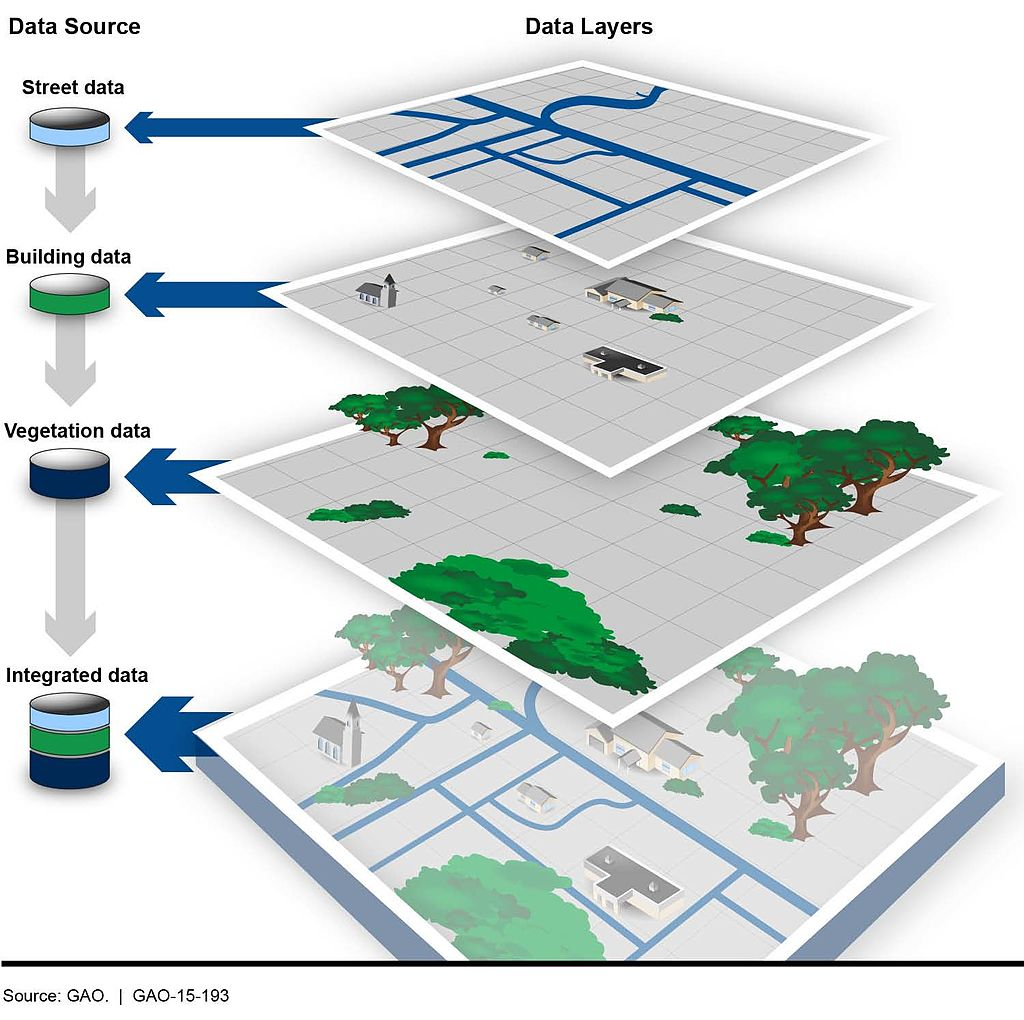
\includegraphics[width=14.22in]{images/geolayers}

\hypertarget{importing-and-viewing-data}{%
\section{Importing and viewing data}\label{importing-and-viewing-data}}

Let's start with the absolute basics of geographic data: loading and viewing.

\begin{Shaded}
\begin{Highlighting}[]
\KeywordTok{library}\NormalTok{(tidyverse)}
\KeywordTok{library}\NormalTok{(sf)}
\KeywordTok{library}\NormalTok{(janitor)}
\end{Highlighting}
\end{Shaded}

First: an aside on geographic data. There are many formats for geographic data, but data type you'll see the most is called the shapefile. It comes from a company named ERSI, which created the most widely used GIS software in the world. For years, they were the only game in town, really, and the shapefile became ubiquitous, especially so in government and utilities. So more often than not, you'll be dealing with a shapefile. But a shapefile isn't just a shapefile -- it's a series of files that combined make up all the data. There's a .shp file -- that's the main file that pulls it all together -- but it's important to note if your shapefiles has a .prj file, which indicates that the projection is specified.

The data we're going to be working with is a file from the Department of Homeland Security that is every hospital in the US and the number of beds they have. I'm writing this during the days of coronavirus, and suddenly the number of hospital beds is a top concern. So let's look at where hospital beds are and how many of them are there. \href{https://unl.box.com/s/o7seh9xqks7gknatihukbdyg6fgbihey}{Download this zipped file and expand it}.

When you do, it should look something like this:

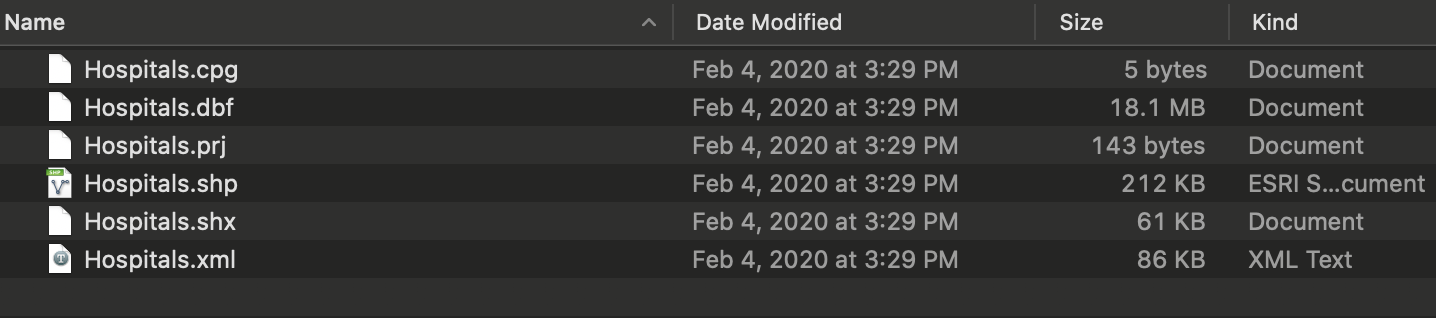
\includegraphics[width=19.94in]{images/geolayers2}

Simlar to \texttt{readr}, the \texttt{sf} library has functions to read geographic data. In this case, we're going to use \texttt{st\_read} to read in our hospitals data.

\begin{Shaded}
\begin{Highlighting}[]
\NormalTok{hospitals <-}\StringTok{ }\KeywordTok{st_read}\NormalTok{(}\StringTok{"data/Hospitals/Hospitals.shp"}\NormalTok{)}
\end{Highlighting}
\end{Shaded}

\begin{verbatim}
## Reading layer `Hospitals' from data source `/Users/mwaite3/Box/BookProjects/DataJournalismWithR/data/Hospitals/Hospitals.shp' using driver `ESRI Shapefile'
## Simple feature collection with 7581 features and 32 fields
## geometry type:  POINT
## dimension:      XY
## bbox:           xmin: -176.6403 ymin: -14.29024 xmax: 145.7245 ymax: 71.29285
## epsg (SRID):    4326
## proj4string:    +proj=longlat +datum=WGS84 +no_defs
\end{verbatim}

From this, we can see that there's 7,581 ``features'', which is the geographic way of saying rows, observations or things. We can see the geometry type is a POINT, which means if we map this we'll see dots where our hospitals are.

But let's not do that. Really, 7500 dots on a map tells you nothing. Let's look at just Nebraska. Good news -- \texttt{sf} plays very nicely with the tidyverse, so we can filter data the way we are accustomed.

\begin{Shaded}
\begin{Highlighting}[]
\NormalTok{ne <-}\StringTok{ }\NormalTok{hospitals }\OperatorTok\StringTok{ }\KeywordTok{filter}\NormalTok{(STATE }\OperatorTok{==}\StringTok{ "NE"}\NormalTok{)}
\end{Highlighting}
\end{Shaded}

What kind of hospitals do we have?

\begin{Shaded}
\begin{Highlighting}[]
\NormalTok{ne }\OperatorTok\StringTok{ }\KeywordTok{tabyl}\NormalTok{(TYPE)}
\end{Highlighting}
\end{Shaded}

\begin{verbatim}
##        TYPEgeometry  n     percent
##            CHILDREN  3 0.027027027
##     CHRONIC DISEASE  0 0.000000000
##     CRITICAL ACCESS 67 0.603603604
##  GENERAL ACUTE CARE 26 0.234234234
##      LONG TERM CARE  3 0.027027027
##            MILITARY  2 0.018018018
##         PSYCHIATRIC  5 0.045045045
##      REHABILITATION  2 0.018018018
##             SPECIAL  2 0.018018018
##               WOMEN  1 0.009009009
\end{verbatim}

Okay, we can safely say that psychiatric, rehabilitation, special, long term care and other types of hospitals are not exactly going to be helpful in this pandemic. We just want CRITICAL ACCESS and GENERAL ACUTE CARE hospitals, which is what we usually associate with a hospital, and are open..

\begin{Shaded}
\begin{Highlighting}[]
\NormalTok{nehospitals <-}\StringTok{ }\NormalTok{ne }\OperatorTok\StringTok{ }\KeywordTok{filter}\NormalTok{(TYPE }\OperatorTok{==}\StringTok{ "CRITICAL ACCESS"} \OperatorTok{|}\StringTok{ }\NormalTok{TYPE }\OperatorTok{==}\StringTok{ "GENERAL ACUTE CARE"}\NormalTok{) }\OperatorTok\StringTok{ }\KeywordTok{filter}\NormalTok{(STATUS }\OperatorTok{==}\StringTok{ "OPEN"}\NormalTok{)}
\end{Highlighting}
\end{Shaded}

That gives us 90 hospitals in Nebraska. Where are they? We can simply plot them using ggplot.

\begin{Shaded}
\begin{Highlighting}[]
\KeywordTok{ggplot}\NormalTok{() }\OperatorTok{+}\StringTok{ }\KeywordTok{geom_sf}\NormalTok{(}\DataTypeTok{data=}\NormalTok{nehospitals) }\OperatorTok{+}\StringTok{ }\KeywordTok{theme_minimal}\NormalTok{()}
\end{Highlighting}
\end{Shaded}

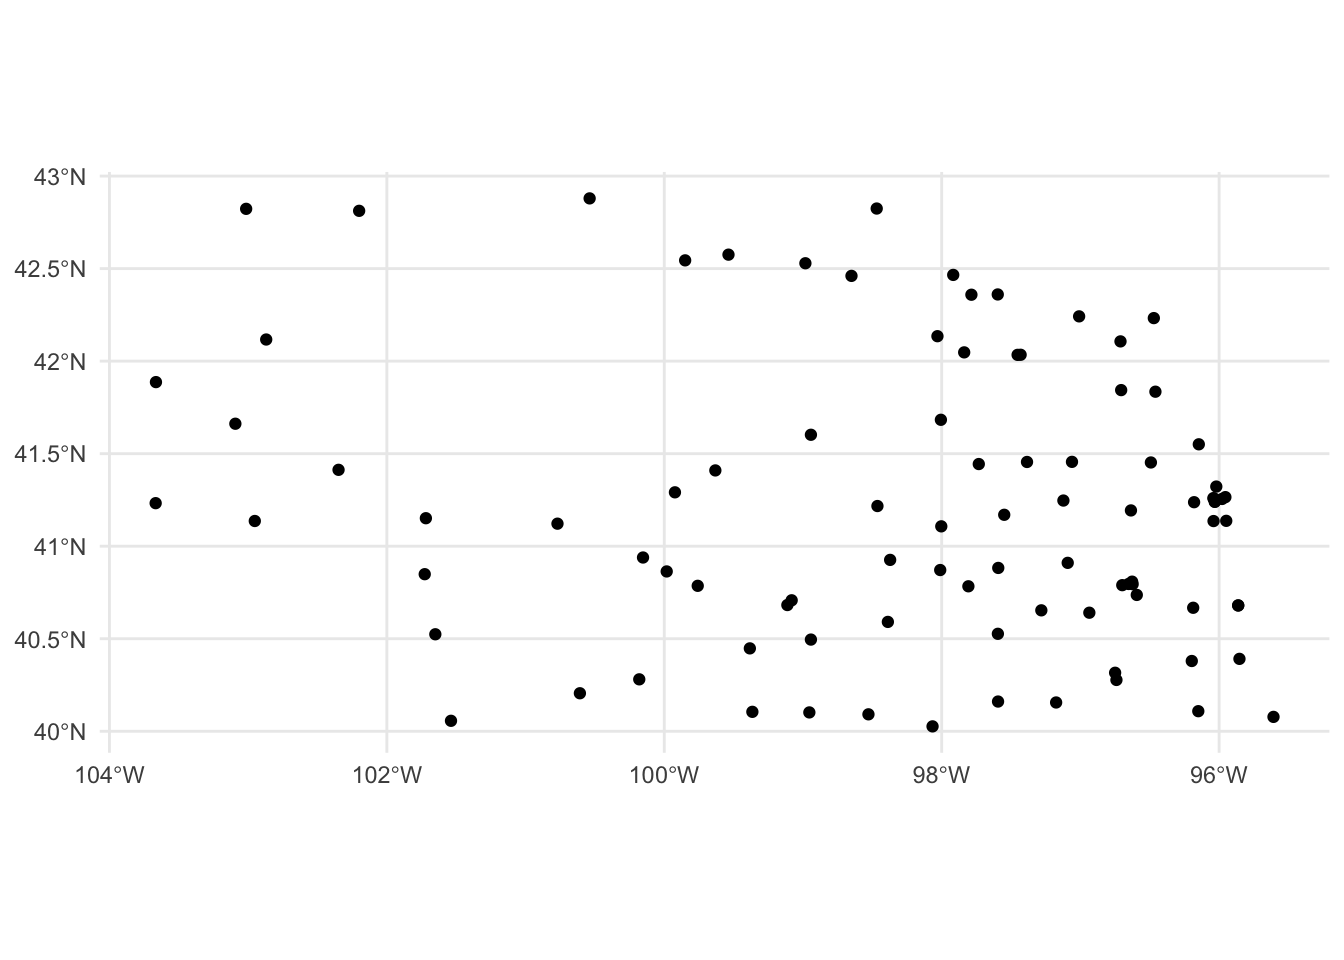
\includegraphics{datajournalism_files/figure-latex/unnamed-chunk-178-1.pdf}

If you know anything about the state of Nebraska, you can kinda pick out the shape of the state there. But that's not exactly ideal.

This is where layering becomes more clear.

Download \href{https://unl.box.com/s/bgvm2x2wzu66mp5o6qykx1flxzz765dj}{this file of county boundaries}. We can read it the same way.

\begin{Shaded}
\begin{Highlighting}[]
\NormalTok{counties <-}\StringTok{ }\KeywordTok{st_read}\NormalTok{(}\StringTok{"data/cb_2018_us_county_5m/cb_2018_us_county_5m.shp"}\NormalTok{)}
\end{Highlighting}
\end{Shaded}

\begin{verbatim}
## Reading layer `cb_2018_us_county_5m' from data source `/Users/mwaite3/Box/BookProjects/DataJournalismWithR/data/cb_2018_us_county_5m/cb_2018_us_county_5m.shp' using driver `ESRI Shapefile'
## Simple feature collection with 3233 features and 9 fields
## geometry type:  MULTIPOLYGON
## dimension:      XY
## bbox:           xmin: -179.1473 ymin: -14.55255 xmax: 179.7785 ymax: 71.35256
## epsg (SRID):    4269
## proj4string:    +proj=longlat +ellps=GRS80 +towgs84=0,0,0,0,0,0,0 +no_defs
\end{verbatim}

And we can filter it the same way. Remember Nebraska's FIPS code from the fatal accident data earlier in the book?

\begin{Shaded}
\begin{Highlighting}[]
\NormalTok{necounties <-}\StringTok{ }\NormalTok{counties }\OperatorTok\StringTok{ }\KeywordTok{filter}\NormalTok{(STATEFP }\OperatorTok{==}\StringTok{ "31"}\NormalTok{)}
\end{Highlighting}
\end{Shaded}

And now we can layer them in. Something to note: The layers are rendered in the order they appear. So the first geom\_sf is rendered first. The second geom\_sf is rendered ON TOP OF the first one.

So if we want to see where hospitals are in Nebraska, we add the counties, then the hospitals.

\begin{Shaded}
\begin{Highlighting}[]
\KeywordTok{ggplot}\NormalTok{() }\OperatorTok{+}\StringTok{ }\KeywordTok{geom_sf}\NormalTok{(}\DataTypeTok{data=}\NormalTok{necounties) }\OperatorTok{+}\StringTok{ }\KeywordTok{geom_sf}\NormalTok{(}\DataTypeTok{data=}\NormalTok{nehospitals) }\OperatorTok{+}\StringTok{ }\KeywordTok{theme_minimal}\NormalTok{()}
\end{Highlighting}
\end{Shaded}

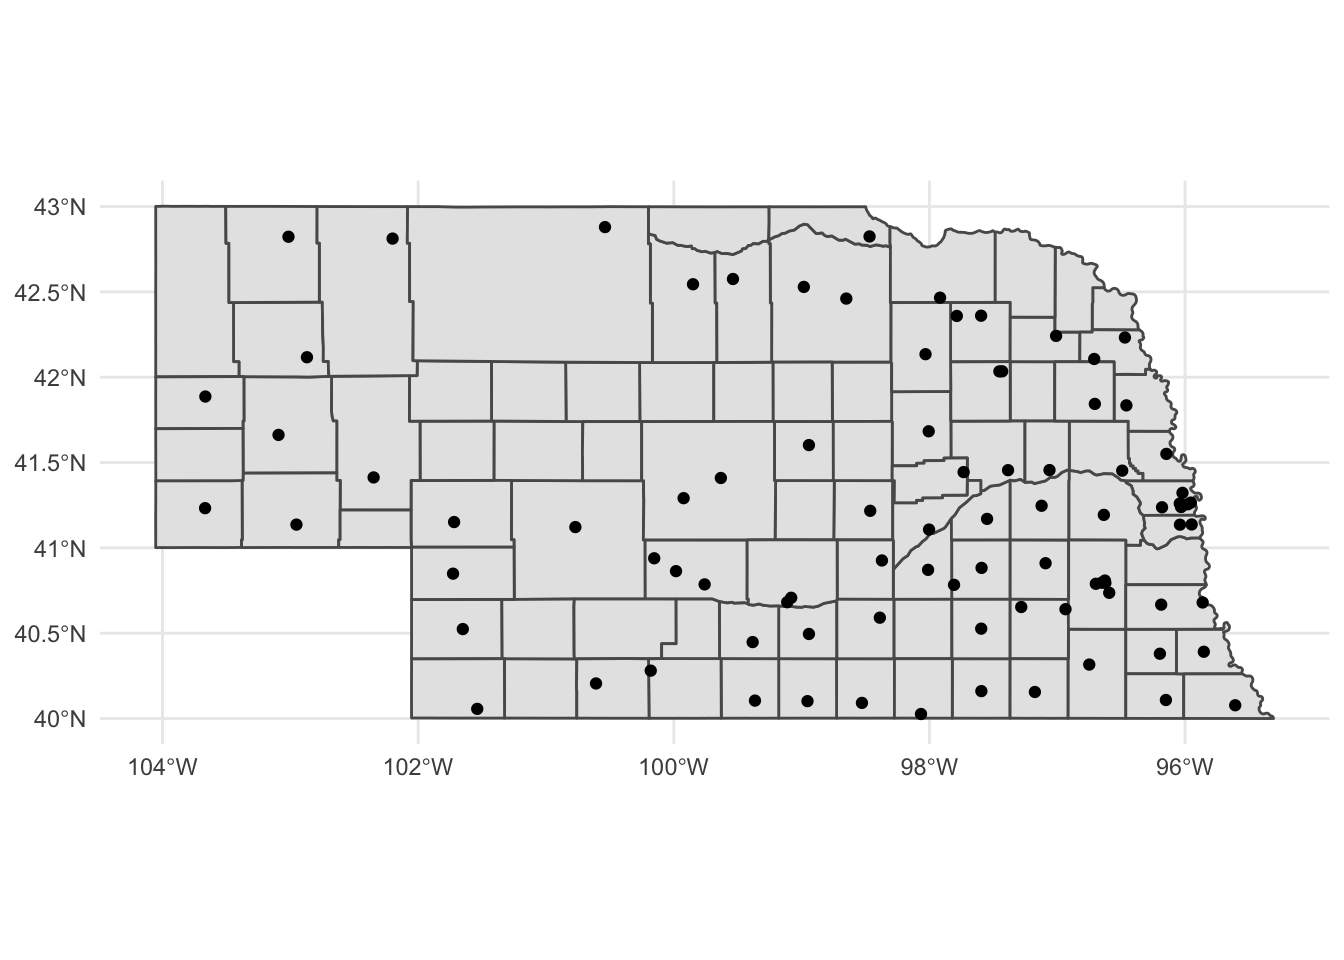
\includegraphics{datajournalism_files/figure-latex/unnamed-chunk-181-1.pdf}

And with that, we can see some questions already arising. How many counties don't have hospitals at all? How many beds are there in each county? What if we had towns as points. Could we find the town that's the farthest from a hospital?

\hypertarget{geographic-analysis}{%
\chapter{Geographic analysis}\label{geographic-analysis}}

In the previous chapter, we looked at Nebraska's hospitals and used layers to show where hospitals on a map of Nebraska's counties. Let's go little further.

First, we get caught up to where we were last time.

\begin{Shaded}
\begin{Highlighting}[]
\KeywordTok{library}\NormalTok{(tidyverse)}
\KeywordTok{library}\NormalTok{(sf)}
\KeywordTok{library}\NormalTok{(janitor)}
\KeywordTok{library}\NormalTok{(scales)}
\end{Highlighting}
\end{Shaded}

\begin{Shaded}
\begin{Highlighting}[]
\NormalTok{hospitals <-}\StringTok{ }\KeywordTok{st_read}\NormalTok{(}\StringTok{"data/Hospitals/Hospitals.shp"}\NormalTok{)}
\end{Highlighting}
\end{Shaded}

\begin{verbatim}
## Reading layer `Hospitals' from data source `/Users/mwaite3/Box/BookProjects/DataJournalismWithR/data/Hospitals/Hospitals.shp' using driver `ESRI Shapefile'
## Simple feature collection with 7581 features and 32 fields
## geometry type:  POINT
## dimension:      XY
## bbox:           xmin: -176.6403 ymin: -14.29024 xmax: 145.7245 ymax: 71.29285
## epsg (SRID):    4326
## proj4string:    +proj=longlat +datum=WGS84 +no_defs
\end{verbatim}

\begin{Shaded}
\begin{Highlighting}[]
\NormalTok{ne <-}\StringTok{ }\NormalTok{hospitals }\OperatorTok\StringTok{ }\KeywordTok{filter}\NormalTok{(STATE }\OperatorTok{==}\StringTok{ "NE"}\NormalTok{)}
\end{Highlighting}
\end{Shaded}

\begin{Shaded}
\begin{Highlighting}[]
\NormalTok{nehospitals <-}\StringTok{ }\NormalTok{ne }\OperatorTok\StringTok{ }\KeywordTok{filter}\NormalTok{(TYPE }\OperatorTok{==}\StringTok{ "CRITICAL ACCESS"} \OperatorTok{|}\StringTok{ }\NormalTok{TYPE }\OperatorTok{==}\StringTok{ "GENERAL ACUTE CARE"}\NormalTok{) }\OperatorTok\StringTok{ }\KeywordTok{filter}\NormalTok{(STATUS }\OperatorTok{==}\StringTok{ "OPEN"}\NormalTok{)}
\end{Highlighting}
\end{Shaded}

\begin{Shaded}
\begin{Highlighting}[]
\NormalTok{counties <-}\StringTok{ }\KeywordTok{st_read}\NormalTok{(}\StringTok{"data/cb_2018_us_county_5m/cb_2018_us_county_5m.shp"}\NormalTok{)}
\end{Highlighting}
\end{Shaded}

\begin{verbatim}
## Reading layer `cb_2018_us_county_5m' from data source `/Users/mwaite3/Box/BookProjects/DataJournalismWithR/data/cb_2018_us_county_5m/cb_2018_us_county_5m.shp' using driver `ESRI Shapefile'
## Simple feature collection with 3233 features and 9 fields
## geometry type:  MULTIPOLYGON
## dimension:      XY
## bbox:           xmin: -179.1473 ymin: -14.55255 xmax: 179.7785 ymax: 71.35256
## epsg (SRID):    4269
## proj4string:    +proj=longlat +ellps=GRS80 +towgs84=0,0,0,0,0,0,0 +no_defs
\end{verbatim}

\begin{Shaded}
\begin{Highlighting}[]
\NormalTok{necounties <-}\StringTok{ }\NormalTok{counties }\OperatorTok\StringTok{ }\KeywordTok{filter}\NormalTok{(STATEFP }\OperatorTok{==}\StringTok{ "31"}\NormalTok{)}
\end{Highlighting}
\end{Shaded}

Now that we're in the same place as last time, let's start asking questions of this data. For starters: how many hopsital beds are there in each county?

At first, we can look at the \texttt{nehospitals} data and see there's a \texttt{COUNTY} field that would make for an easy group and summarize.

\begin{Shaded}
\begin{Highlighting}[]
\NormalTok{nehospitals }\OperatorTok\StringTok{ }\KeywordTok{group_by}\NormalTok{(COUNTY) }\OperatorTok\StringTok{ }\KeywordTok{summarize}\NormalTok{(}\DataTypeTok{total_beds=}\KeywordTok{sum}\NormalTok{(BEDS))}
\end{Highlighting}
\end{Shaded}

\begin{verbatim}
## Simple feature collection with 67 features and 2 fields
## geometry type:  GEOMETRY
## dimension:      XY
## bbox:           xmin: -103.6668 ymin: 40.02644 xmax: -95.60789 ymax: 42.87939
## epsg (SRID):    4326
## proj4string:    +proj=longlat +datum=WGS84 +no_defs
## # A tibble: 67 x 3
##    COUNTY    total_beds                                            geometry
##  * <fct>          <dbl>                                      <GEOMETRY [°]>
##  1 ADAMS            161                          POINT (-98.38807 40.59091)
##  2 ANTELOPE          25                          POINT (-98.03064 42.13475)
##  3 BOONE             25                          POINT (-98.00574 41.68304)
##  4 BOX BUTTE         25                          POINT (-102.8699 42.11684)
##  5 BOYD              20                          POINT (-98.46849 42.82457)
##  6 BROWN             23                          POINT (-99.84956 42.54451)
##  7 BUFFALO          261 MULTIPOINT (-99.11259 40.68205, -99.08158 40.70766)
##  8 BURT              18                          POINT (-96.45918 41.83485)
##  9 BUTLER            20                          POINT (-97.12253 41.24669)
## 10 CHASE             22                          POINT (-101.6507 40.52413)
## # ... with 57 more rows
\end{verbatim}

But look at Thurston County. How does a county have a negative number of hospital beds? When DHS doesn't know and can't find it, they put in -999 to indicate unknown. That's \ldots{} obivously not good for us, so we need to filter that.

Also, notice we still get a geometry? That's because \texttt{nehospitals} isn't a dataframe -- it's a simple features file. So that geometry is coming with, regardless. Except in this case, it's useless. It's a collection of points. It does us no good.

What we really want to do with this data is join the number of beds in each county to the county map, and then shade those counties by the number of beds. It's a style of map called a cloropleth map. You've seen them before.

To do that, we need to make a dataframe. In our our hospitals data, we have a field called COUNTYFIPS that is identical to the GEOID in the counties data -- it's the merging of the state fips and the county fips to make a unique number for each county. So in one query, we need to convert our \texttt{sf} file to a dataframe, filter out the -999 hospital, group it by the COUNTY and COUNTYFIPS and then, to save us some hassle, we're going to rename that COUNTYFIPS field to GEOID which makes our join easier. And, as one last convenience, we're going to drop the geometry, because that too will cause confusion.

Follow? No worries if you didn't. Each step by itself is simple, and they add up together.

\begin{Shaded}
\begin{Highlighting}[]
\NormalTok{nebedcount <-}\StringTok{ }
\StringTok{  }\KeywordTok{as.data.frame}\NormalTok{(}
\NormalTok{    nehospitals }\OperatorTok\StringTok{ }
\StringTok{      }\KeywordTok{filter}\NormalTok{(BEDS }\OperatorTok{!=}\StringTok{ }\DecValTok{-999}\NormalTok{) }\OperatorTok\StringTok{ }
\StringTok{      }\KeywordTok{group_by}\NormalTok{(COUNTY, COUNTYFIPS) }\OperatorTok\StringTok{ }
\StringTok{      }\KeywordTok{summarize}\NormalTok{(}\DataTypeTok{total_beds =} \KeywordTok{sum}\NormalTok{(BEDS)}
\NormalTok{  ) }\OperatorTok\StringTok{ }
\StringTok{    }\KeywordTok{rename}\NormalTok{(}\DataTypeTok{GEOID =}\NormalTok{ COUNTYFIPS)) }\OperatorTok\StringTok{ }
\StringTok{  }\KeywordTok{select}\NormalTok{(}\OperatorTok{-}\NormalTok{geometry)}
\end{Highlighting}
\end{Shaded}

Let's take a look at what we got:

\begin{Shaded}
\begin{Highlighting}[]
\KeywordTok{head}\NormalTok{(nebedcount)}
\end{Highlighting}
\end{Shaded}

\begin{verbatim}
##      COUNTY GEOID total_beds
## 1     ADAMS 31001        161
## 2  ANTELOPE 31003         25
## 3     BOONE 31011         25
## 4 BOX BUTTE 31013         25
## 5      BOYD 31015         20
## 6     BROWN 31017         23
\end{verbatim}

Pretty simple. Three columns: COUNTY, GEOID and total\_beds.

Now using what we learned in the joining chapter, we can combine them with our counties data.

\begin{Shaded}
\begin{Highlighting}[]
\NormalTok{nehospbycounty <-}\StringTok{ }\NormalTok{necounties }\OperatorTok\StringTok{ }\KeywordTok{left_join}\NormalTok{(nebedcount, }\DataTypeTok{by=}\StringTok{"GEOID"}\NormalTok{)}
\end{Highlighting}
\end{Shaded}

\begin{verbatim}
## Warning: Column `GEOID` joining factors with different levels, coercing to
## character vector
\end{verbatim}

We can ignore that warning.

Now we can map it. What's going to change here is we're going to add a fill to our aes in our geom\_sf.

\begin{Shaded}
\begin{Highlighting}[]
\KeywordTok{ggplot}\NormalTok{() }\OperatorTok{+}\StringTok{ }
\StringTok{  }\KeywordTok{geom_sf}\NormalTok{(}\DataTypeTok{data=}\NormalTok{nehospbycounty, }\KeywordTok{aes}\NormalTok{(}\DataTypeTok{fill=}\NormalTok{total_beds)) }\OperatorTok{+}\StringTok{ }
\StringTok{  }\KeywordTok{theme_minimal}\NormalTok{()}
\end{Highlighting}
\end{Shaded}

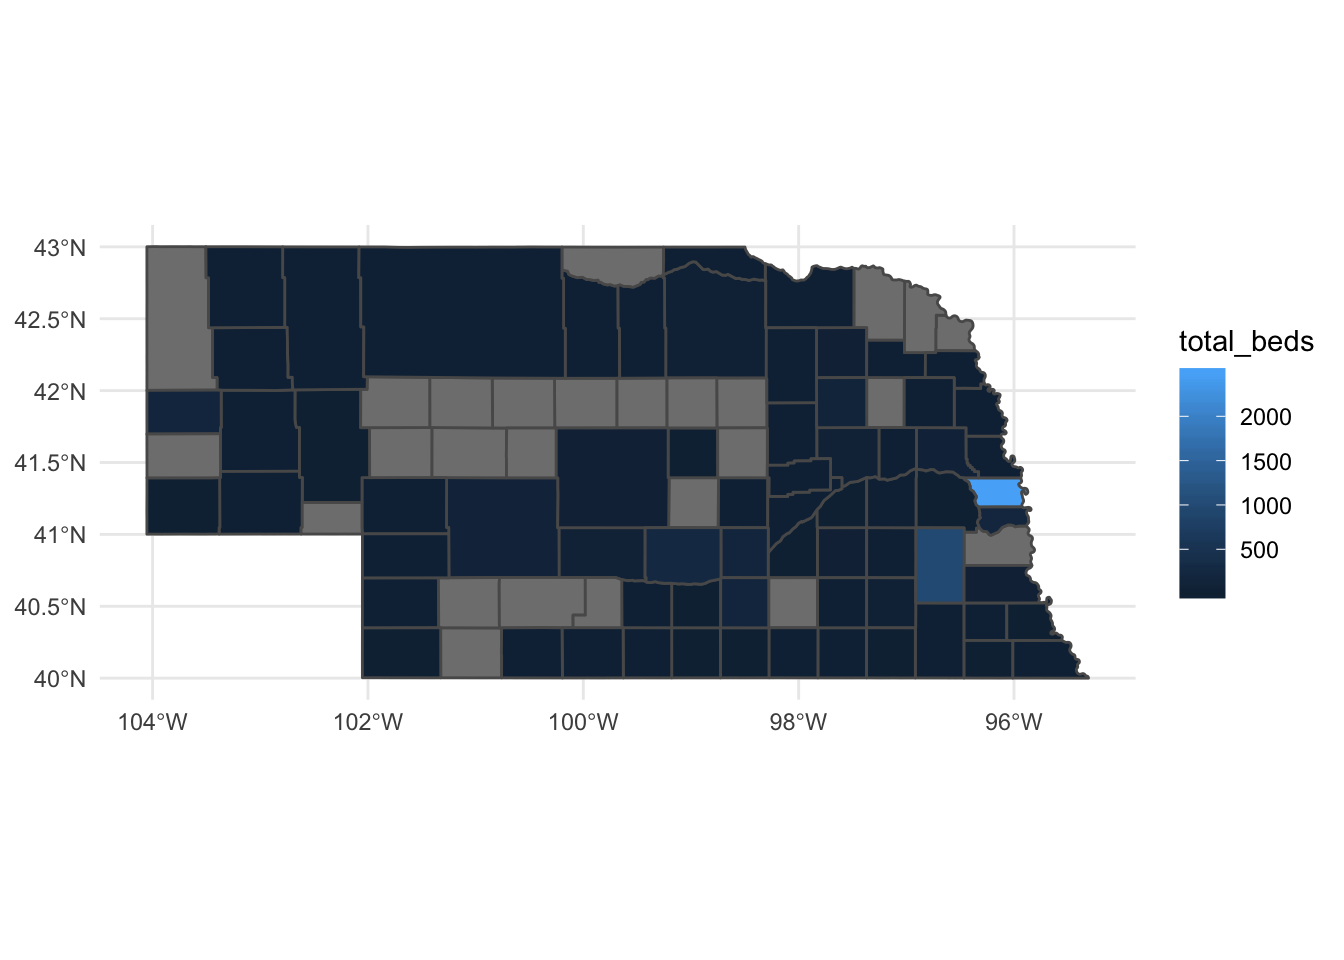
\includegraphics{datajournalism_files/figure-latex/unnamed-chunk-192-1.pdf}

We get what we expect \ldots{} it's not ideal. We can't really tell a difference between anything outside of Douglas and Lancaster counties. So we can add a scale in here. This one is called viridis, and it makes a more visibile color ramp. And since we have a large disparity between Douglas County and pretty much everywhere else, we'll make the scale exponential.

\begin{Shaded}
\begin{Highlighting}[]
\KeywordTok{ggplot}\NormalTok{() }\OperatorTok{+}\StringTok{ }
\StringTok{  }\KeywordTok{geom_sf}\NormalTok{(}\DataTypeTok{data=}\NormalTok{nehospbycounty, }\KeywordTok{aes}\NormalTok{(}\DataTypeTok{fill=}\NormalTok{total_beds)) }\OperatorTok{+}\StringTok{ }
\StringTok{  }\KeywordTok{theme_minimal}\NormalTok{() }\OperatorTok{+}\StringTok{ }
\StringTok{  }\KeywordTok{scale_fill_viridis_c}\NormalTok{(}\DataTypeTok{option =} \StringTok{"plasma"}\NormalTok{, }\DataTypeTok{trans =} \StringTok{"sqrt"}\NormalTok{)}
\end{Highlighting}
\end{Shaded}

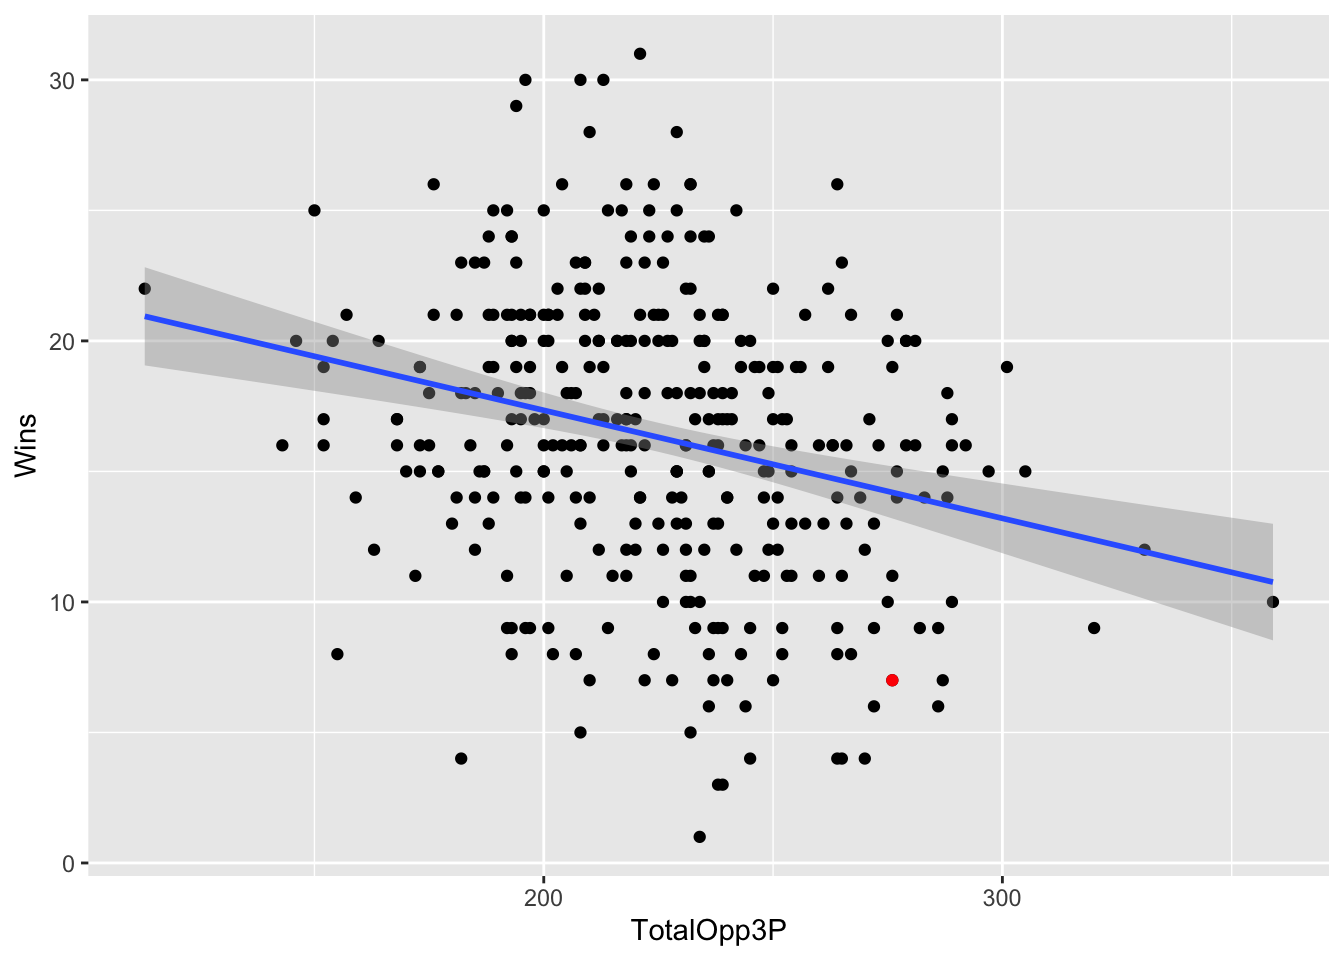
\includegraphics{datajournalism_files/figure-latex/unnamed-chunk-193-1.pdf}

So there's the map. How about a list:

\begin{Shaded}
\begin{Highlighting}[]
\NormalTok{nebedcount }\OperatorTok\StringTok{ }\KeywordTok{select}\NormalTok{(COUNTY, total_beds) }\OperatorTok\StringTok{ }\KeywordTok{arrange}\NormalTok{(}\KeywordTok{desc}\NormalTok{(total_beds)) }
\end{Highlighting}
\end{Shaded}

\begin{verbatim}
##          COUNTY total_beds
## 1       DOUGLAS       2479
## 2     LANCASTER        984
## 3       BUFFALO        261
## 4         SARPY        176
## 5  SCOTTS BLUFF        166
## 6         ADAMS        161
## 7          HALL        159
## 8       MADISON        131
## 9       LINCOLN        116
## 10        DODGE         81
## 11       DAWSON         58
## 12       PLATTE         51
## 13         HOLT         43
## 14       SALINE         43
## 15       PIERCE         40
## 16         YORK         38
## 17         OTOE         36
## 18       CUSTER         35
## 19     ANTELOPE         25
## 20        BOONE         25
## 21    BOX BUTTE         25
## 22       CHERRY         25
## 23     CHEYENNE         25
## 24       COLFAX         25
## 25       CUMING         25
## 26        DAWES         25
## 27         GAGE         25
## 28       HOWARD         25
## 29     NUCKOLLS         25
## 30       PHELPS         25
## 31   RED WILLOW         25
## 32     SHERIDAN         25
## 33   WASHINGTON         25
## 34        WAYNE         25
## 35   RICHARDSON         24
## 36         ROCK         24
## 37       SEWARD         24
## 38        BROWN         23
## 39         KNOX         23
## 40        CHASE         22
## 41     THURSTON         21
## 42         BOYD         20
## 43       BUTLER         20
## 44     FILLMORE         20
## 45       FURNAS         20
## 46      MERRICK         20
## 47      MORRILL         20
## 48      PERKINS         20
## 49       HARLAN         19
## 50        NANCE         19
## 51       THAYER         19
## 52         BURT         18
## 53      JOHNSON         18
## 54        KEITH         18
## 55    JEFFERSON         17
## 56       NEMAHA         16
## 57         POLK         16
## 58     SAUNDERS         16
## 59       VALLEY         16
## 60        DUNDY         14
## 61     FRANKLIN         14
## 62     HAMILTON         14
## 63      WEBSTER         13
## 64      KIMBALL         12
## 65       PAWNEE         11
## 66       GARDEN         10
## 67      KEARNEY         10
\end{verbatim}

So there's a lot of hosptial beds in Omaha (DOUGLAS) and Lincoln (LANCASTER). Some quick math shows there 3,463 beds in those two counties. How many beds are in the rest of the state combined?

\begin{Shaded}
\begin{Highlighting}[]
\NormalTok{nebedcount }\OperatorTok\StringTok{ }\KeywordTok{filter}\NormalTok{(COUNTY }\OperatorTok{!=}\StringTok{ "DOUGLAS"} \OperatorTok{&}\StringTok{ }\NormalTok{COUNTY }\OperatorTok{!=}\StringTok{ "LANCASTER"}\NormalTok{) }\OperatorTok\StringTok{ }\KeywordTok{summarize}\NormalTok{(}\KeywordTok{sum}\NormalTok{(total_beds))}
\end{Highlighting}
\end{Shaded}

\begin{verbatim}
##   sum(total_beds)
## 1            2586
\end{verbatim}

How many total beds?

\begin{Shaded}
\begin{Highlighting}[]
\NormalTok{nebedcount }\OperatorTok\StringTok{ }\KeywordTok{summarize}\NormalTok{(}\KeywordTok{sum}\NormalTok{(total_beds))}
\end{Highlighting}
\end{Shaded}

\begin{verbatim}
##   sum(total_beds)
## 1            6049
\end{verbatim}

So there's 6,104 beds in the state and 3,463 of them are in Omaha and Lincoln. What perent is that?

\begin{Shaded}
\begin{Highlighting}[]
\DecValTok{3463}\OperatorTok{/}\DecValTok{6104}
\end{Highlighting}
\end{Shaded}

\begin{verbatim}
## [1] 0.5673329
\end{verbatim}

According to this data, 57 percent of the state's hospital beds are in two counties. What about population?

\hypertarget{why-tidycensus-is-so-useful}{%
\section{Why tidycensus is so useful}\label{why-tidycensus-is-so-useful}}

Most of the time when we're looking at population questions, we're looking at Census data. So what percent of people live in Lancaster and Douglas counties?

\begin{Shaded}
\begin{Highlighting}[]
\KeywordTok{library}\NormalTok{(tidycensus)}
\end{Highlighting}
\end{Shaded}

In this case, the population variable we're looking for is Total Population, which is \texttt{B01003\_001} and we're looking at the county geography. Here's what that looks like:

\begin{Shaded}
\begin{Highlighting}[]
\NormalTok{nepop <-}\StringTok{ }\KeywordTok{get_acs}\NormalTok{(}\DataTypeTok{geography =} \StringTok{"county"}\NormalTok{, }
              \DataTypeTok{variables =} \KeywordTok{c}\NormalTok{(}\DataTypeTok{population =} \StringTok{"B01003_001"}\NormalTok{), }
              \DataTypeTok{state =} \StringTok{"NE"}\NormalTok{, }
              \DataTypeTok{year =} \DecValTok{2018}\NormalTok{)}
\end{Highlighting}
\end{Shaded}

\begin{verbatim}
## Getting data from the 2014-2018 5-year ACS
\end{verbatim}

First we can filter FOR Douglas OR Lancaster using the \textbar{} character:

\begin{Shaded}
\begin{Highlighting}[]
\NormalTok{nepop }\OperatorTok\StringTok{ }\KeywordTok{filter}\NormalTok{(NAME }\OperatorTok{==}\StringTok{ "Lancaster County, Nebraska"} \OperatorTok{|}\StringTok{ }\NormalTok{NAME }\OperatorTok{==}\StringTok{ "Douglas County, Nebraska"}\NormalTok{) }\OperatorTok\StringTok{ }\KeywordTok{summarize}\NormalTok{(}\KeywordTok{sum}\NormalTok{(estimate))}
\end{Highlighting}
\end{Shaded}

\begin{verbatim}
## # A tibble: 1 x 1
##   `sum(estimate)`
##             <dbl>
## 1          865086
\end{verbatim}

Now without them:

\begin{Shaded}
\begin{Highlighting}[]
\NormalTok{nepop }\OperatorTok\StringTok{ }\KeywordTok{filter}\NormalTok{(NAME }\OperatorTok{!=}\StringTok{ "Lancaster County, Nebraska"} \OperatorTok{|}\StringTok{ }\NormalTok{NAME }\OperatorTok{!=}\StringTok{ "Douglas County, Nebraska"}\NormalTok{) }\OperatorTok\StringTok{ }\KeywordTok{summarize}\NormalTok{(}\KeywordTok{sum}\NormalTok{(estimate))}
\end{Highlighting}
\end{Shaded}

\begin{verbatim}
## # A tibble: 1 x 1
##   `sum(estimate)`
##             <dbl>
## 1         1904760
\end{verbatim}

All together now:

\begin{Shaded}
\begin{Highlighting}[]
\NormalTok{nepop }\OperatorTok\StringTok{ }\KeywordTok{summarize}\NormalTok{(}\KeywordTok{sum}\NormalTok{(estimate))}
\end{Highlighting}
\end{Shaded}

\begin{verbatim}
## # A tibble: 1 x 1
##   `sum(estimate)`
##             <dbl>
## 1         1904760
\end{verbatim}

And the percentage:

\begin{Shaded}
\begin{Highlighting}[]
\DecValTok{865086}\OperatorTok{/}\DecValTok{1904760}
\end{Highlighting}
\end{Shaded}

\begin{verbatim}
## [1] 0.4541706
\end{verbatim}

So Omaha and Lincoln represent 57 percent of the hospital beds, but only 45 percent of the population.

\hypertarget{automating-analysis}{%
\chapter{Automating analysis}\label{automating-analysis}}

Many of the data analyses that you do will be largely one-off efforts -- you're going to do the analysis and write the story and be done. Maybe you'll come back to it in a couple of months or years, but really you're just doing it once.

But what happens when you have a long-running story, where you're going to update it every day, or every week? What changes when you're writing that code?

\begin{enumerate}
\def\labelenumi{\arabic{enumi}.}
\tightlist
\item
  How will this run again without changing anything?
\item
  What questions do you have that have to be answered each time?
\item
  What changes when you have to repeat questions to changing data?
\end{enumerate}

The global COVID-19 pandemic is something we're going to be writing about and covering for some time. One element of it -- one that materialized in Nebraska as I am writing this -- is a tsunami of first time joblessness claims for unemployment assistance. That data is regularly published, and we're going to be talking about it weekly for a long time. So it's the ideal candidate for repeating analysis -- scripting the questions we want to answer every week and doing so in a way that we can just load it without having to change anything.

Let's get some new libraries to our typical tidyverse import. First, I'm going to add a library called \texttt{readxl}, which does what you think it does. It reads Microsoft Excel files. The next one I'm going to add is \texttt{DT}. It stands for datatables, and it makes your dataframes into html tables that are browsable and searchable. This is a bigger issue for me -- the author who is turning these into html pages -- than you, working in your notebooks. We're also going to add a library called ggrepel, which assists in putting tables on dots in charts.

You install them the same way you do anything else -- \texttt{install.packages("readxl")} and \texttt{install.packages("DT")} and \texttt{install.packages("ggrepel")}.

\begin{Shaded}
\begin{Highlighting}[]
\KeywordTok{library}\NormalTok{(tidyverse)}
\KeywordTok{library}\NormalTok{(janitor)}
\KeywordTok{library}\NormalTok{(readxl)}
\KeywordTok{library}\NormalTok{(DT)}
\KeywordTok{library}\NormalTok{(ggrepel)}
\end{Highlighting}
\end{Shaded}

\hypertarget{automating-downloads-an-imports}{%
\section{Automating downloads an imports}\label{automating-downloads-an-imports}}

Nebraska \href{https://neworks.nebraska.gov/gsipub/index.asp?docid=710}{publishes data weekly on first time unemployment claims on a Department of Labor website}.

There's four datasets. We're looking at the weekly initial claims from 2012 to present. If you click it, you'll get an Excel spreadsheet. That's a problem, given that we've been working with CSVs all along. So the problem we have before us is this: Have to download it first, then open an Excel file with multiple sheets and lots of header and footers.

There's a multitude of ways to get data from a website, but base R has a simple function to just download a file and name it. Couldn't be easier. Right or control click on the link for the 2012 to 2020 initial claims data and copy the link location. Then use this function:

\begin{Shaded}
\begin{Highlighting}[]
\KeywordTok{download.file}\NormalTok{(}\StringTok{"https://neworks.nebraska.gov/admin/gsipub/htmlarea/uploads/NE%20UI%20Weekly%20Initial%20Claims.xlsx"}\NormalTok{, }\DataTypeTok{destfile =} \StringTok{"weeklyinitialclaims.xlsx"}\NormalTok{)}
\end{Highlighting}
\end{Shaded}

Open the file in Excel so you can see what we're working with. The first sheet is just definitions and explanations. Then each sheet is a year (or year to date) of data. Some have footers. Some don't. Some have a headline. Some don't. So we have some work ahead of us.

There are better ways to do this, and if your author was better at this, I'd tell you about it. But for beginners and people who aren't totally sure of themselves, explicit is better than implicit. So instead of using programming magic, we're going to use copy and paste. My programmer friends just died inside a little, but done is better than clever.

What we need to do, in words, is this:

\begin{enumerate}
\def\labelenumi{\arabic{enumi}.}
\tightlist
\item
  Read a specific sheet
\item
  Skip the top row
\item
  Clean the column names with janitor.
\item
  Select just the first two rows, which will help us chop out some garbage.
\item
  We need to find if the sheet has that source line at the end of the data, so we'll use \texttt{str\_detect} in \texttt{stringr} and filter it out.
\item
  We'll use janitor to remove any empty rows and columns
\item
  And lastly, we'll convert all the numbers in initial\_claims to actual numbers, because the Source line made them character on import.
\end{enumerate}

It's a lot, but not really. Each step is very simple, and is designed to solve one problem. And after we do it with one, we'll do it with the next, and the next, and the next, so on and so forth.

\begin{Shaded}
\begin{Highlighting}[]
\NormalTok{weeklyclaims20 <-}\StringTok{ }\KeywordTok{read_excel}\NormalTok{(}\StringTok{"weeklyinitialclaims.xlsx"}\NormalTok{, }\DataTypeTok{sheet=}\DecValTok{2}\NormalTok{, }\DataTypeTok{skip=}\DecValTok{1}\NormalTok{) }\OperatorTok\StringTok{ }
\StringTok{  }\KeywordTok{clean_names}\NormalTok{() }\OperatorTok\StringTok{ }
\StringTok{  }\KeywordTok{select}\NormalTok{(}\DecValTok{1}\OperatorTok{:}\DecValTok{2}\NormalTok{) }\OperatorTok\StringTok{ }
\StringTok{  }\KeywordTok{filter}\NormalTok{(}\OperatorTok{!}\KeywordTok{str_detect}\NormalTok{(initial_claims, }\StringTok{"Source"}\NormalTok{)) }\OperatorTok\StringTok{  }
\StringTok{  }\KeywordTok{remove_empty}\NormalTok{(}\KeywordTok{c}\NormalTok{(}\StringTok{"cols"}\NormalTok{, }\StringTok{"rows"}\NormalTok{)) }\OperatorTok\StringTok{ }
\StringTok{  }\KeywordTok{mutate}\NormalTok{(}\DataTypeTok{initial_claims =} \KeywordTok{as.numeric}\NormalTok{(initial_claims))}
\end{Highlighting}
\end{Shaded}

\begin{verbatim}
## New names:
## * `` -> ...3
## * `` -> ...4
## * `` -> ...5
\end{verbatim}

\begin{Shaded}
\begin{Highlighting}[]
\NormalTok{weeklyclaims19 <-}\StringTok{ }\KeywordTok{read_excel}\NormalTok{(}\StringTok{"weeklyinitialclaims.xlsx"}\NormalTok{, }\DataTypeTok{sheet=}\DecValTok{3}\NormalTok{, }\DataTypeTok{skip=}\DecValTok{1}\NormalTok{) }\OperatorTok
\StringTok{  }\KeywordTok{clean_names}\NormalTok{() }\OperatorTok\StringTok{ }\KeywordTok{select}\NormalTok{(}\DecValTok{1}\OperatorTok{:}\DecValTok{2}\NormalTok{) }\OperatorTok
\StringTok{  }\KeywordTok{filter}\NormalTok{(}\OperatorTok{!}\KeywordTok{str_detect}\NormalTok{(initial_claims, }\StringTok{"Source"}\NormalTok{)) }\OperatorTok
\StringTok{  }\KeywordTok{remove_empty}\NormalTok{(}\KeywordTok{c}\NormalTok{(}\StringTok{"cols"}\NormalTok{, }\StringTok{"rows"}\NormalTok{)) }\OperatorTok
\StringTok{  }\KeywordTok{mutate}\NormalTok{(}\DataTypeTok{initial_claims =} \KeywordTok{as.numeric}\NormalTok{(initial_claims))}
\end{Highlighting}
\end{Shaded}

\begin{verbatim}
## New names:
## * `` -> ...3
## * `` -> ...4
## * `` -> ...5
\end{verbatim}

\begin{Shaded}
\begin{Highlighting}[]
\NormalTok{weeklyclaims18 <-}\StringTok{ }\KeywordTok{read_excel}\NormalTok{(}\StringTok{"weeklyinitialclaims.xlsx"}\NormalTok{, }\DataTypeTok{sheet=}\DecValTok{4}\NormalTok{, }\DataTypeTok{skip=}\DecValTok{1}\NormalTok{) }\OperatorTok
\StringTok{  }\KeywordTok{clean_names}\NormalTok{() }\OperatorTok
\StringTok{  }\KeywordTok{select}\NormalTok{(}\DecValTok{1}\OperatorTok{:}\DecValTok{2}\NormalTok{) }\OperatorTok
\StringTok{  }\KeywordTok{filter}\NormalTok{(}\OperatorTok{!}\KeywordTok{str_detect}\NormalTok{(initial_claims, }\StringTok{"Source"}\NormalTok{)) }\OperatorTok
\StringTok{  }\KeywordTok{remove_empty}\NormalTok{(}\KeywordTok{c}\NormalTok{(}\StringTok{"cols"}\NormalTok{, }\StringTok{"rows"}\NormalTok{)) }\OperatorTok
\StringTok{  }\KeywordTok{mutate}\NormalTok{(}\DataTypeTok{initial_claims =} \KeywordTok{as.numeric}\NormalTok{(initial_claims))}

\NormalTok{weeklyclaims17 <-}\StringTok{ }\KeywordTok{read_excel}\NormalTok{(}\StringTok{"weeklyinitialclaims.xlsx"}\NormalTok{, }\DataTypeTok{sheet=}\DecValTok{5}\NormalTok{, }\DataTypeTok{skip=}\DecValTok{1}\NormalTok{) }\OperatorTok
\StringTok{  }\KeywordTok{clean_names}\NormalTok{() }\OperatorTok
\StringTok{  }\KeywordTok{select}\NormalTok{(}\DecValTok{1}\OperatorTok{:}\DecValTok{2}\NormalTok{) }\OperatorTok
\StringTok{  }\KeywordTok{filter}\NormalTok{(}\OperatorTok{!}\KeywordTok{str_detect}\NormalTok{(initial_claims, }\StringTok{"Source"}\NormalTok{)) }\OperatorTok
\StringTok{  }\KeywordTok{remove_empty}\NormalTok{(}\KeywordTok{c}\NormalTok{(}\StringTok{"cols"}\NormalTok{, }\StringTok{"rows"}\NormalTok{)) }\OperatorTok
\StringTok{  }\KeywordTok{mutate}\NormalTok{(}\DataTypeTok{initial_claims =} \KeywordTok{as.numeric}\NormalTok{(initial_claims))}

\NormalTok{weeklyclaims16 <-}\StringTok{ }\KeywordTok{read_excel}\NormalTok{(}\StringTok{"weeklyinitialclaims.xlsx"}\NormalTok{, }\DataTypeTok{sheet=}\DecValTok{6}\NormalTok{, }\DataTypeTok{skip=}\DecValTok{1}\NormalTok{) }\OperatorTok
\StringTok{  }\KeywordTok{clean_names}\NormalTok{() }\OperatorTok
\StringTok{  }\KeywordTok{select}\NormalTok{(}\DecValTok{1}\OperatorTok{:}\DecValTok{2}\NormalTok{) }\OperatorTok
\StringTok{  }\KeywordTok{filter}\NormalTok{(}\OperatorTok{!}\KeywordTok{str_detect}\NormalTok{(initial_claims, }\StringTok{"Source"}\NormalTok{)) }\OperatorTok
\StringTok{  }\KeywordTok{remove_empty}\NormalTok{(}\KeywordTok{c}\NormalTok{(}\StringTok{"cols"}\NormalTok{, }\StringTok{"rows"}\NormalTok{)) }\OperatorTok
\StringTok{  }\KeywordTok{mutate}\NormalTok{(}\DataTypeTok{initial_claims =} \KeywordTok{as.numeric}\NormalTok{(initial_claims))}

\NormalTok{weeklyclaims15 <-}\StringTok{ }\KeywordTok{read_excel}\NormalTok{(}\StringTok{"weeklyinitialclaims.xlsx"}\NormalTok{, }\DataTypeTok{sheet=}\DecValTok{7}\NormalTok{, }\DataTypeTok{skip=}\DecValTok{1}\NormalTok{) }\OperatorTok
\StringTok{  }\KeywordTok{clean_names}\NormalTok{() }\OperatorTok
\StringTok{  }\KeywordTok{select}\NormalTok{(}\DecValTok{1}\OperatorTok{:}\DecValTok{2}\NormalTok{) }\OperatorTok
\StringTok{  }\KeywordTok{filter}\NormalTok{(}\OperatorTok{!}\KeywordTok{str_detect}\NormalTok{(initial_claims, }\StringTok{"Source"}\NormalTok{)) }\OperatorTok
\StringTok{  }\KeywordTok{remove_empty}\NormalTok{(}\KeywordTok{c}\NormalTok{(}\StringTok{"cols"}\NormalTok{, }\StringTok{"rows"}\NormalTok{)) }\OperatorTok
\StringTok{  }\KeywordTok{mutate}\NormalTok{(}\DataTypeTok{initial_claims =} \KeywordTok{as.numeric}\NormalTok{(initial_claims))}

\NormalTok{weeklyclaims14 <-}\StringTok{ }\KeywordTok{read_excel}\NormalTok{(}\StringTok{"weeklyinitialclaims.xlsx"}\NormalTok{, }\DataTypeTok{sheet=}\DecValTok{8}\NormalTok{, }\DataTypeTok{skip=}\DecValTok{1}\NormalTok{) }\OperatorTok
\StringTok{  }\KeywordTok{clean_names}\NormalTok{() }\OperatorTok
\StringTok{  }\KeywordTok{select}\NormalTok{(}\DecValTok{1}\OperatorTok{:}\DecValTok{2}\NormalTok{) }\OperatorTok
\StringTok{  }\KeywordTok{filter}\NormalTok{(}\OperatorTok{!}\KeywordTok{str_detect}\NormalTok{(initial_claims, }\StringTok{"Source"}\NormalTok{)) }\OperatorTok
\StringTok{  }\KeywordTok{remove_empty}\NormalTok{(}\KeywordTok{c}\NormalTok{(}\StringTok{"cols"}\NormalTok{, }\StringTok{"rows"}\NormalTok{)) }\OperatorTok
\StringTok{  }\KeywordTok{mutate}\NormalTok{(}\DataTypeTok{initial_claims =} \KeywordTok{as.numeric}\NormalTok{(initial_claims))}

\NormalTok{weeklyclaims13 <-}\StringTok{ }\KeywordTok{read_excel}\NormalTok{(}\StringTok{"weeklyinitialclaims.xlsx"}\NormalTok{, }\DataTypeTok{sheet=}\DecValTok{9}\NormalTok{, }\DataTypeTok{skip=}\DecValTok{1}\NormalTok{) }\OperatorTok
\StringTok{  }\KeywordTok{clean_names}\NormalTok{() }\OperatorTok
\StringTok{  }\KeywordTok{select}\NormalTok{(}\DecValTok{1}\OperatorTok{:}\DecValTok{2}\NormalTok{) }\OperatorTok
\StringTok{  }\KeywordTok{filter}\NormalTok{(}\OperatorTok{!}\KeywordTok{str_detect}\NormalTok{(initial_claims, }\StringTok{"Source"}\NormalTok{)) }\OperatorTok
\StringTok{  }\KeywordTok{remove_empty}\NormalTok{(}\KeywordTok{c}\NormalTok{(}\StringTok{"cols"}\NormalTok{, }\StringTok{"rows"}\NormalTok{)) }\OperatorTok
\StringTok{  }\KeywordTok{mutate}\NormalTok{(}\DataTypeTok{initial_claims =} \KeywordTok{as.numeric}\NormalTok{(initial_claims))}

\NormalTok{weeklyclaims12 <-}\StringTok{ }\KeywordTok{read_excel}\NormalTok{(}\StringTok{"weeklyinitialclaims.xlsx"}\NormalTok{, }\DataTypeTok{sheet=}\DecValTok{10}\NormalTok{, }\DataTypeTok{skip=}\DecValTok{1}\NormalTok{) }\OperatorTok
\StringTok{  }\KeywordTok{clean_names}\NormalTok{() }\OperatorTok
\StringTok{  }\KeywordTok{select}\NormalTok{(}\DecValTok{1}\OperatorTok{:}\DecValTok{2}\NormalTok{) }\OperatorTok
\StringTok{  }\KeywordTok{filter}\NormalTok{(}\OperatorTok{!}\KeywordTok{str_detect}\NormalTok{(initial_claims, }\StringTok{"Source"}\NormalTok{)) }\OperatorTok
\StringTok{  }\KeywordTok{remove_empty}\NormalTok{(}\KeywordTok{c}\NormalTok{(}\StringTok{"cols"}\NormalTok{, }\StringTok{"rows"}\NormalTok{)) }\OperatorTok
\StringTok{  }\KeywordTok{mutate}\NormalTok{(}\DataTypeTok{initial_claims =} \KeywordTok{as.numeric}\NormalTok{(initial_claims))}
\end{Highlighting}
\end{Shaded}

Now we need to combine all those tables together. We can do that with rbind and some convenient overwriting of a dataframe to add new data each time.

\begin{Shaded}
\begin{Highlighting}[]
\NormalTok{weeklyclaims <-}\StringTok{ }\KeywordTok{rbind}\NormalTok{(weeklyclaims12, weeklyclaims13)}
\NormalTok{weeklyclaims <-}\StringTok{ }\KeywordTok{rbind}\NormalTok{(weeklyclaims, weeklyclaims14)}
\NormalTok{weeklyclaims <-}\StringTok{ }\KeywordTok{rbind}\NormalTok{(weeklyclaims, weeklyclaims15)}
\NormalTok{weeklyclaims <-}\StringTok{ }\KeywordTok{rbind}\NormalTok{(weeklyclaims, weeklyclaims16)}
\NormalTok{weeklyclaims <-}\StringTok{ }\KeywordTok{rbind}\NormalTok{(weeklyclaims, weeklyclaims17)}
\NormalTok{weeklyclaims <-}\StringTok{ }\KeywordTok{rbind}\NormalTok{(weeklyclaims, weeklyclaims18)}
\NormalTok{weeklyclaims <-}\StringTok{ }\KeywordTok{rbind}\NormalTok{(weeklyclaims, weeklyclaims19)}
\NormalTok{weeklyclaims <-}\StringTok{ }\KeywordTok{rbind}\NormalTok{(weeklyclaims, weeklyclaims20)}
\end{Highlighting}
\end{Shaded}

\hypertarget{exploring-the-data}{%
\section{Exploring the data}\label{exploring-the-data}}

Let's take a look at what we have, using datatables. The formatDate business just makes the date look nicer.

\begin{Shaded}
\begin{Highlighting}[]
\KeywordTok{datatable}\NormalTok{(weeklyclaims) }\OperatorTok\StringTok{ }\KeywordTok{formatDate}\NormalTok{(}\DecValTok{1}\NormalTok{, }\StringTok{"toLocaleDateString"}\NormalTok{)}
\end{Highlighting}
\end{Shaded}

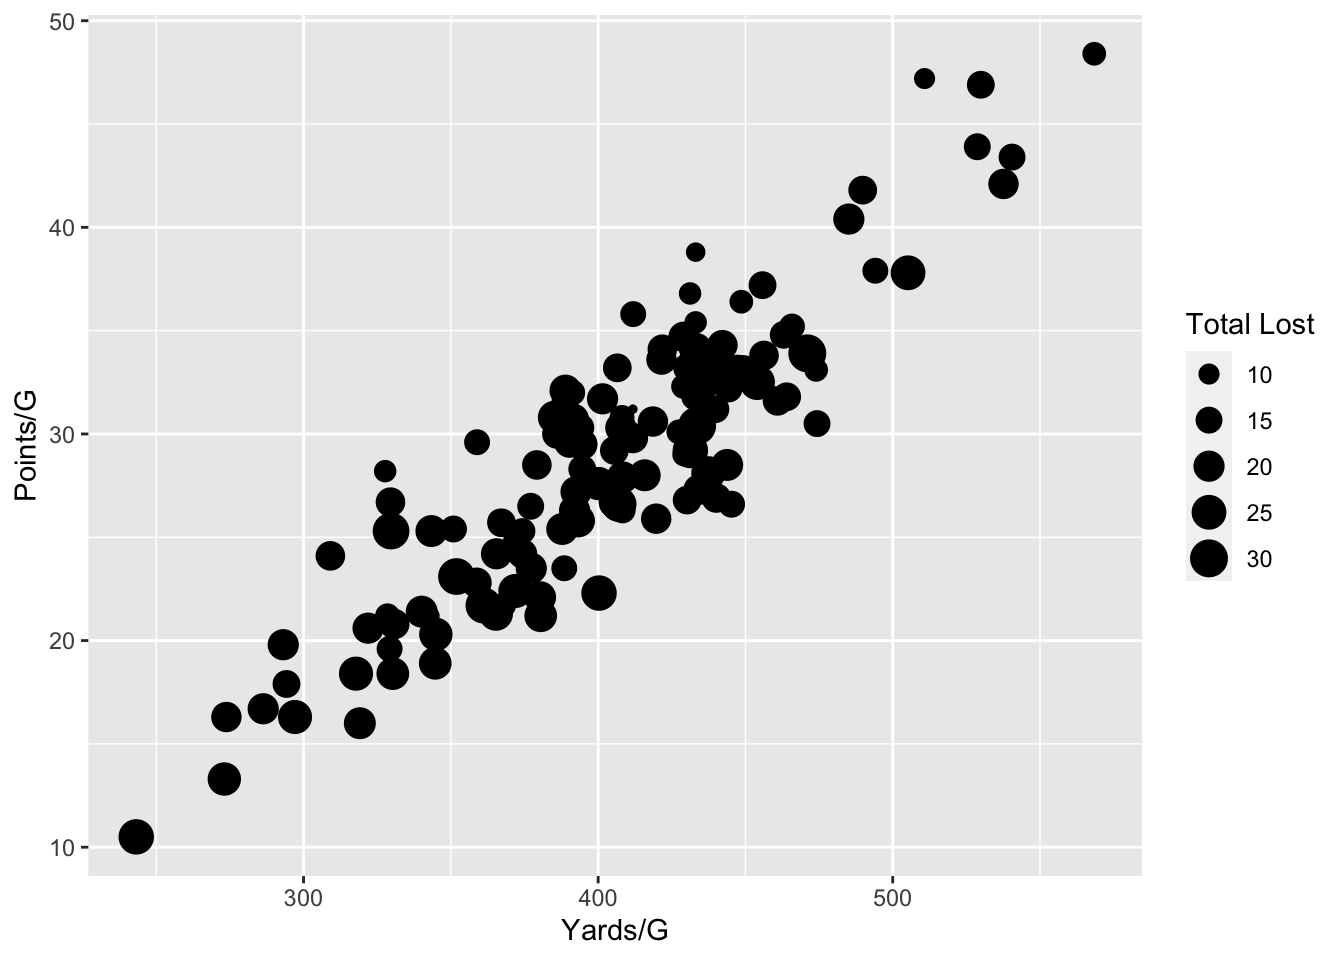
\includegraphics{datajournalism_files/figure-latex/unnamed-chunk-208-1.pdf}

Let's just look at the most recent week, and that's something that takes on different meaning when we're talking about updating data. We need to make this generic so that every time we pull this up and run it, it's the most recent week at the top. This time, it's very simple.

\begin{Shaded}
\begin{Highlighting}[]
\NormalTok{weeklyclaims20 }\OperatorTok\StringTok{ }\KeywordTok{arrange}\NormalTok{(}\KeywordTok{desc}\NormalTok{(week_ending_date))}
\end{Highlighting}
\end{Shaded}

\begin{verbatim}
## # A tibble: 11 x 2
##    week_ending_date    initial_claims
##    <dttm>                       <dbl>
##  1 2020-03-14 00:00:00            763
##  2 2020-03-07 00:00:00            498
##  3 2020-02-29 00:00:00            496
##  4 2020-02-22 00:00:00            476
##  5 2020-02-15 00:00:00            527
##  6 2020-02-08 00:00:00            653
##  7 2020-02-01 00:00:00            796
##  8 2020-01-25 00:00:00            916
##  9 2020-01-18 00:00:00            913
## 10 2020-01-11 00:00:00           1036
## 11 2020-01-04 00:00:00           1089
\end{verbatim}

\hypertarget{analysis}{%
\section{Analysis}\label{analysis}}

Now is when we need to start asking ourselves -- what are the questions that are going to come up week after week. What about how this most current week compares to all weeks going back to 2012? What if we just ranked them? Where does this week rank? For that, we'll create a new column called Rank using mutate and we'll use a function called \texttt{min\_rank} to rank them. I'm going to save them to a dataframe and use data

\begin{Shaded}
\begin{Highlighting}[]
\NormalTok{ranked <-}\StringTok{ }\NormalTok{weeklyclaims }\OperatorTok\StringTok{ }\KeywordTok{mutate}\NormalTok{(}\DataTypeTok{Rank =} \KeywordTok{min_rank}\NormalTok{(}\KeywordTok{desc}\NormalTok{(initial_claims))) }\OperatorTok\StringTok{ }\KeywordTok{arrange}\NormalTok{(}\KeywordTok{desc}\NormalTok{(week_ending_date)) }

\KeywordTok{datatable}\NormalTok{(ranked) }\OperatorTok\StringTok{ }\KeywordTok{formatDate}\NormalTok{(}\DecValTok{1}\NormalTok{, }\StringTok{"toLocaleDateString"}\NormalTok{) }
\end{Highlighting}
\end{Shaded}

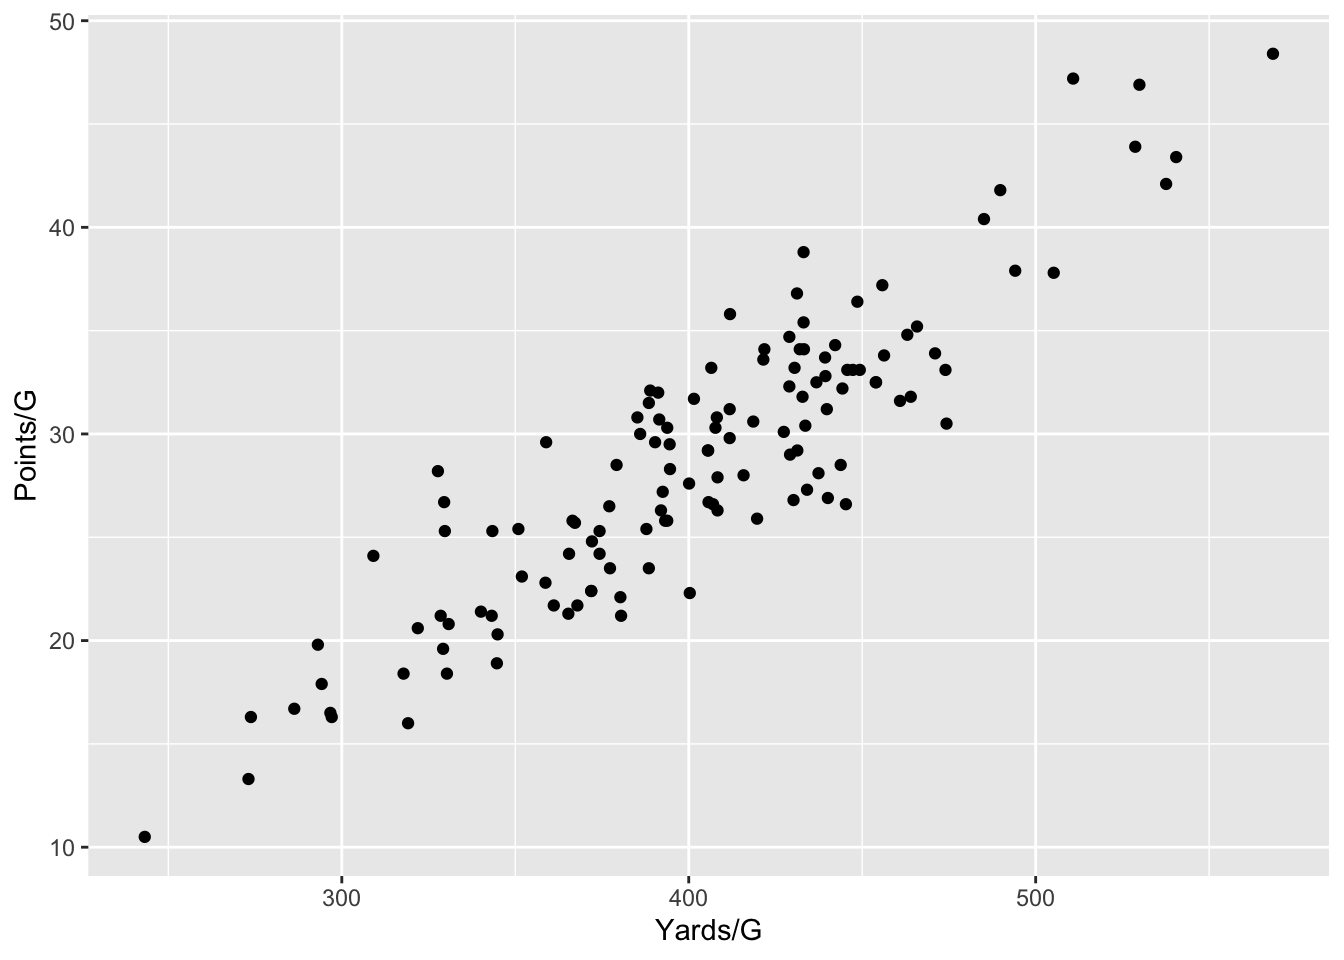
\includegraphics{datajournalism_files/figure-latex/unnamed-chunk-210-1.pdf}

Let's think about this a little more. What else could we do with this. What are the recurring questions? How about the percent change between this week and last week?

To do that, we need our dates to be next to each other -- side by side. Then we can do new minus old divided by old. To do that, we're going to use a function from \texttt{tidyr} called pivot\_wider, which will transform our data from one row per week to one row, with the weeks as columns.

\begin{Shaded}
\begin{Highlighting}[]
\NormalTok{change <-}\StringTok{ }\NormalTok{weeklyclaims20 }\OperatorTok\StringTok{ }\KeywordTok{pivot_wider}\NormalTok{(}\DataTypeTok{names_from =}\NormalTok{ week_ending_date, }\DataTypeTok{values_from =}\NormalTok{ initial_claims)}

\KeywordTok{head}\NormalTok{(change)}
\end{Highlighting}
\end{Shaded}

\begin{verbatim}
## # A tibble: 1 x 11
##   `2020-01-04` `2020-01-11` `2020-01-18` `2020-01-25` `2020-02-01` `2020-02-08`
##          <dbl>        <dbl>        <dbl>        <dbl>        <dbl>        <dbl>
## 1         1089         1036          913          916          796          653
## # ... with 5 more variables: `2020-02-15` <dbl>, `2020-02-22` <dbl>,
## #   `2020-02-29` <dbl>, `2020-03-07` <dbl>, `2020-03-14` <dbl>
\end{verbatim}

Now the problem we have is \ldots{} which column is the last one, and which one is the previous one? I'll be honest, this isn't easy in R. But the trick is to reverse the order of the columns. Then, your newest one is column 1 and the next newest is 2.

\begin{Shaded}
\begin{Highlighting}[]
\NormalTok{changecalc <-}\StringTok{ }\NormalTok{((}\KeywordTok{rev}\NormalTok{(change)[}\DecValTok{1}\NormalTok{] }\OperatorTok{-}\StringTok{ }\KeywordTok{rev}\NormalTok{(change)[}\DecValTok{2}\NormalTok{])}\OperatorTok{/}\KeywordTok{rev}\NormalTok{(change)[}\DecValTok{2}\NormalTok{])}\OperatorTok{*}\DecValTok{100}

\NormalTok{changecalc}
\end{Highlighting}
\end{Shaded}

\begin{verbatim}
##   2020-03-14
## 1   53.21285
\end{verbatim}

So whatever the date, that'll always return the percent change between the most recent date and the previous week.

\hypertarget{making-updating-graphics}{%
\section{Making updating graphics}\label{making-updating-graphics}}

More than numbers, we are going to want to see this data. We can build this in steps. First, let's just make a big bar chart.

\begin{Shaded}
\begin{Highlighting}[]
\KeywordTok{ggplot}\NormalTok{() }\OperatorTok{+}\StringTok{ }
\StringTok{  }\KeywordTok{geom_bar}\NormalTok{(}\DataTypeTok{data=}\NormalTok{ranked, }\KeywordTok{aes}\NormalTok{(}\DataTypeTok{x=}\NormalTok{week_ending_date, }\DataTypeTok{weight=}\NormalTok{initial_claims)) }
\end{Highlighting}
\end{Shaded}

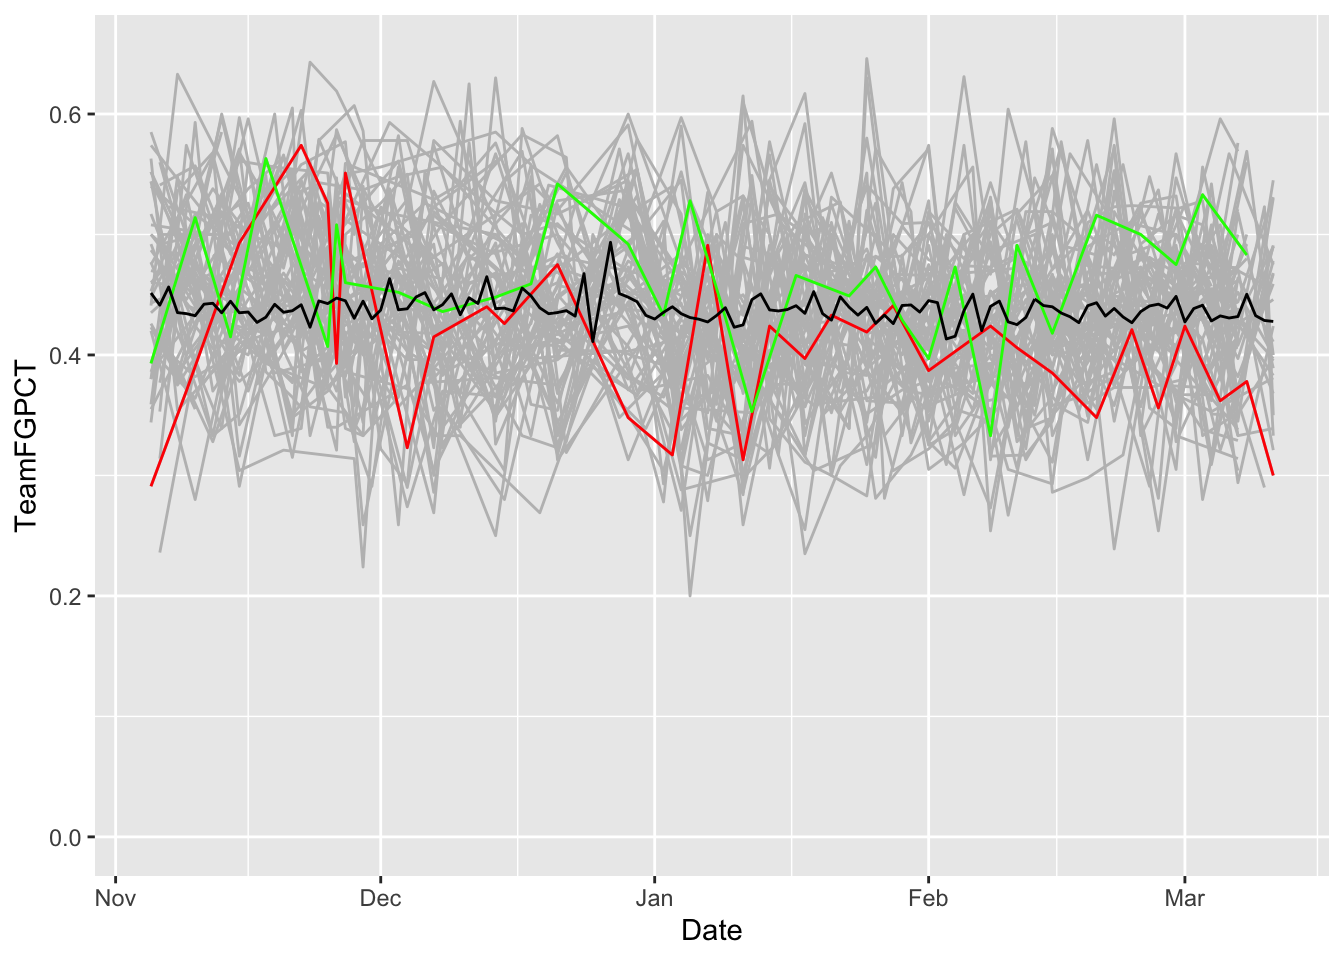
\includegraphics{datajournalism_files/figure-latex/unnamed-chunk-213-1.pdf}

So that shows us that the trend is going down over time, and that there's some regular spikes around the holidays. Which tells us this data is seasonal, but we knew that going in.

Let's build up some more layers to highlight trends and the most recent spot.

First, we'll slice out a dataframe that's just the most recent data.

\begin{Shaded}
\begin{Highlighting}[]
\NormalTok{latest <-}\StringTok{ }\NormalTok{ranked }\OperatorTok\StringTok{ }\KeywordTok{slice}\NormalTok{(}\DecValTok{1}\NormalTok{)}
\end{Highlighting}
\end{Shaded}

Now, in ggplot, we can add multiple layers.

The first layer will be all the bars.

The second layer will just be the latest.

Then we'll add a point to the top of that line to really draw attention to it.

Then we'll use ggprepel to label it.

Then I'm going to add a smoothing line. That'll illustrate the trend clearly.

The rest is labeling and adjusting the text to make it look more like a news graphic.

\begin{Shaded}
\begin{Highlighting}[]
\KeywordTok{ggplot}\NormalTok{() }\OperatorTok{+}\StringTok{ }
\StringTok{  }\KeywordTok{geom_bar}\NormalTok{(}\DataTypeTok{data=}\NormalTok{ranked, }\KeywordTok{aes}\NormalTok{(}\DataTypeTok{x=}\NormalTok{week_ending_date, }\DataTypeTok{weight=}\NormalTok{initial_claims)) }\OperatorTok{+}
\StringTok{  }\KeywordTok{geom_bar}\NormalTok{(}\DataTypeTok{data=}\NormalTok{latest, }\KeywordTok{aes}\NormalTok{(}\DataTypeTok{x=}\NormalTok{week_ending_date, }\DataTypeTok{weight=}\NormalTok{initial_claims), }\DataTypeTok{fill=}\StringTok{"red"}\NormalTok{) }\OperatorTok{+}
\StringTok{  }\KeywordTok{geom_point}\NormalTok{(}\DataTypeTok{data=}\NormalTok{latest, }\KeywordTok{aes}\NormalTok{(}\DataTypeTok{x=}\NormalTok{week_ending_date, }\DataTypeTok{y=}\NormalTok{initial_claims)) }\OperatorTok{+}\StringTok{ }
\StringTok{  }\KeywordTok{geom_text_repel}\NormalTok{(}\DataTypeTok{data=}\NormalTok{latest, }\KeywordTok{aes}\NormalTok{(}\DataTypeTok{x=}\NormalTok{week_ending_date, }\DataTypeTok{y=}\NormalTok{initial_claims }\OperatorTok{+}\StringTok{ }\DecValTok{150}\NormalTok{, }\DataTypeTok{label=}\StringTok{"This week"}\NormalTok{)) }\OperatorTok{+}\StringTok{ }
\StringTok{  }\KeywordTok{geom_smooth}\NormalTok{(}\DataTypeTok{data=}\NormalTok{ranked, }\KeywordTok{aes}\NormalTok{(}\DataTypeTok{x=}\NormalTok{week_ending_date, }\DataTypeTok{y=}\NormalTok{initial_claims), }\DataTypeTok{method=}\NormalTok{loess, }\DataTypeTok{se=}\OtherTok{FALSE}\NormalTok{) }\OperatorTok{+}\StringTok{ }
\StringTok{  }\KeywordTok{labs}\NormalTok{(}\DataTypeTok{title=}\StringTok{"Nebraska jobless claims on the rise"}\NormalTok{, }\DataTypeTok{x=}\StringTok{"Date"}\NormalTok{, }\DataTypeTok{y=}\StringTok{"Claims"}\NormalTok{) }\OperatorTok{+}
\StringTok{  }\KeywordTok{theme_minimal}\NormalTok{() }\OperatorTok{+}\StringTok{ }
\StringTok{  }\KeywordTok{theme}\NormalTok{(}
    \DataTypeTok{plot.title =} \KeywordTok{element_text}\NormalTok{(}\DataTypeTok{size =} \DecValTok{16}\NormalTok{, }\DataTypeTok{face =} \StringTok{"bold"}\NormalTok{),}
    \DataTypeTok{axis.title =} \KeywordTok{element_text}\NormalTok{(}\DataTypeTok{size =} \DecValTok{8}\NormalTok{), }
    \DataTypeTok{plot.subtitle =} \KeywordTok{element_text}\NormalTok{(}\DataTypeTok{size=}\DecValTok{10}\NormalTok{), }
    \DataTypeTok{panel.grid.minor =} \KeywordTok{element_blank}\NormalTok{()}
\NormalTok{    )}
\end{Highlighting}
\end{Shaded}

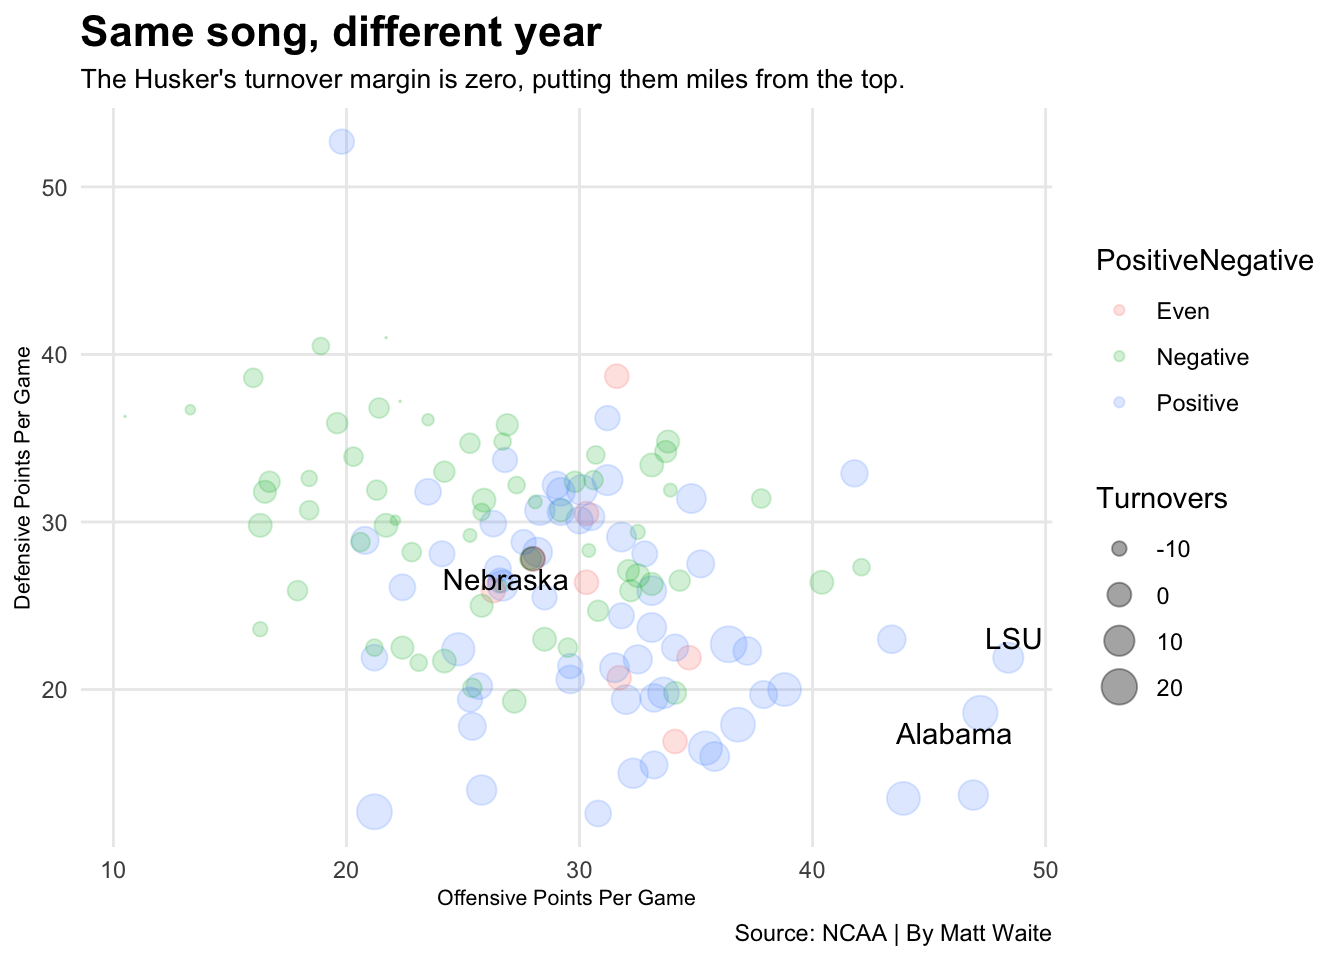
\includegraphics{datajournalism_files/figure-latex/unnamed-chunk-215-1.pdf}

One thing we are missing? Context. What if we programmatically wrote the chatter for this chart using the percent change calculation we did before?

First, we format the change to look more news graphic like and not with 7 significant digits.

\begin{Shaded}
\begin{Highlighting}[]
\NormalTok{changetext <-}\StringTok{ }\KeywordTok{round}\NormalTok{(changecalc[[}\DecValTok{1}\NormalTok{]], }\DataTypeTok{digits=}\DecValTok{2}\NormalTok{)}
\end{Highlighting}
\end{Shaded}

Now we're going to use a function called paste to merge some text together. We're going to paste together a sentence fragment, the percent change number and another sentence fragment together to form a sentence. We'll save it as sub, because that's what it's called in ggplot -- a subtitle.

\begin{Shaded}
\begin{Highlighting}[]
\NormalTok{sub <-}\StringTok{ }\KeywordTok{paste}\NormalTok{(}\StringTok{"First time unemployment claims rose by "}\NormalTok{, changetext, }\StringTok{" percent over last week"}\NormalTok{, }\DataTypeTok{sep=}\StringTok{""}\NormalTok{)}
\end{Highlighting}
\end{Shaded}

Heres's our sentence:

\begin{Shaded}
\begin{Highlighting}[]
\NormalTok{sub}
\end{Highlighting}
\end{Shaded}

\begin{verbatim}
## [1] "First time unemployment claims rose by 53.21 percent over last week"
\end{verbatim}

Now we can add that to our labels.

\begin{Shaded}
\begin{Highlighting}[]
\KeywordTok{ggplot}\NormalTok{() }\OperatorTok{+}\StringTok{ }
\StringTok{  }\KeywordTok{geom_bar}\NormalTok{(}\DataTypeTok{data=}\NormalTok{ranked, }\KeywordTok{aes}\NormalTok{(}\DataTypeTok{x=}\NormalTok{week_ending_date, }\DataTypeTok{weight=}\NormalTok{initial_claims)) }\OperatorTok{+}
\StringTok{  }\KeywordTok{geom_bar}\NormalTok{(}\DataTypeTok{data=}\NormalTok{latest, }\KeywordTok{aes}\NormalTok{(}\DataTypeTok{x=}\NormalTok{week_ending_date, }\DataTypeTok{weight=}\NormalTok{initial_claims), }\DataTypeTok{fill=}\StringTok{"red"}\NormalTok{) }\OperatorTok{+}
\StringTok{  }\KeywordTok{geom_point}\NormalTok{(}\DataTypeTok{data=}\NormalTok{latest, }\KeywordTok{aes}\NormalTok{(}\DataTypeTok{x=}\NormalTok{week_ending_date, }\DataTypeTok{y=}\NormalTok{initial_claims)) }\OperatorTok{+}\StringTok{ }
\StringTok{  }\KeywordTok{geom_text_repel}\NormalTok{(}\DataTypeTok{data=}\NormalTok{latest, }\KeywordTok{aes}\NormalTok{(}\DataTypeTok{x=}\NormalTok{week_ending_date, }\DataTypeTok{y=}\NormalTok{initial_claims }\OperatorTok{+}\StringTok{ }\DecValTok{150}\NormalTok{, }\DataTypeTok{label=}\StringTok{"This week"}\NormalTok{)) }\OperatorTok{+}\StringTok{ }
\StringTok{  }\KeywordTok{geom_smooth}\NormalTok{(}\DataTypeTok{data=}\NormalTok{ranked, }\KeywordTok{aes}\NormalTok{(}\DataTypeTok{x=}\NormalTok{week_ending_date, }\DataTypeTok{y=}\NormalTok{initial_claims), }\DataTypeTok{method=}\NormalTok{loess, }\DataTypeTok{se=}\OtherTok{FALSE}\NormalTok{) }\OperatorTok{+}\StringTok{ }
\StringTok{  }\KeywordTok{labs}\NormalTok{(}\DataTypeTok{title=}\StringTok{"Nebraska jobless claims on the rise"}\NormalTok{, }\DataTypeTok{subtitle=}\NormalTok{sub, }\DataTypeTok{x=}\StringTok{"Date"}\NormalTok{, }\DataTypeTok{y=}\StringTok{"Claims"}\NormalTok{) }\OperatorTok{+}
\StringTok{  }\KeywordTok{theme_minimal}\NormalTok{() }\OperatorTok{+}\StringTok{ }
\StringTok{  }\KeywordTok{theme}\NormalTok{(}
    \DataTypeTok{plot.title =} \KeywordTok{element_text}\NormalTok{(}\DataTypeTok{size =} \DecValTok{16}\NormalTok{, }\DataTypeTok{face =} \StringTok{"bold"}\NormalTok{),}
    \DataTypeTok{axis.title =} \KeywordTok{element_text}\NormalTok{(}\DataTypeTok{size =} \DecValTok{8}\NormalTok{), }
    \DataTypeTok{plot.subtitle =} \KeywordTok{element_text}\NormalTok{(}\DataTypeTok{size=}\DecValTok{10}\NormalTok{), }
    \DataTypeTok{panel.grid.minor =} \KeywordTok{element_blank}\NormalTok{()}
\NormalTok{    )}
\end{Highlighting}
\end{Shaded}

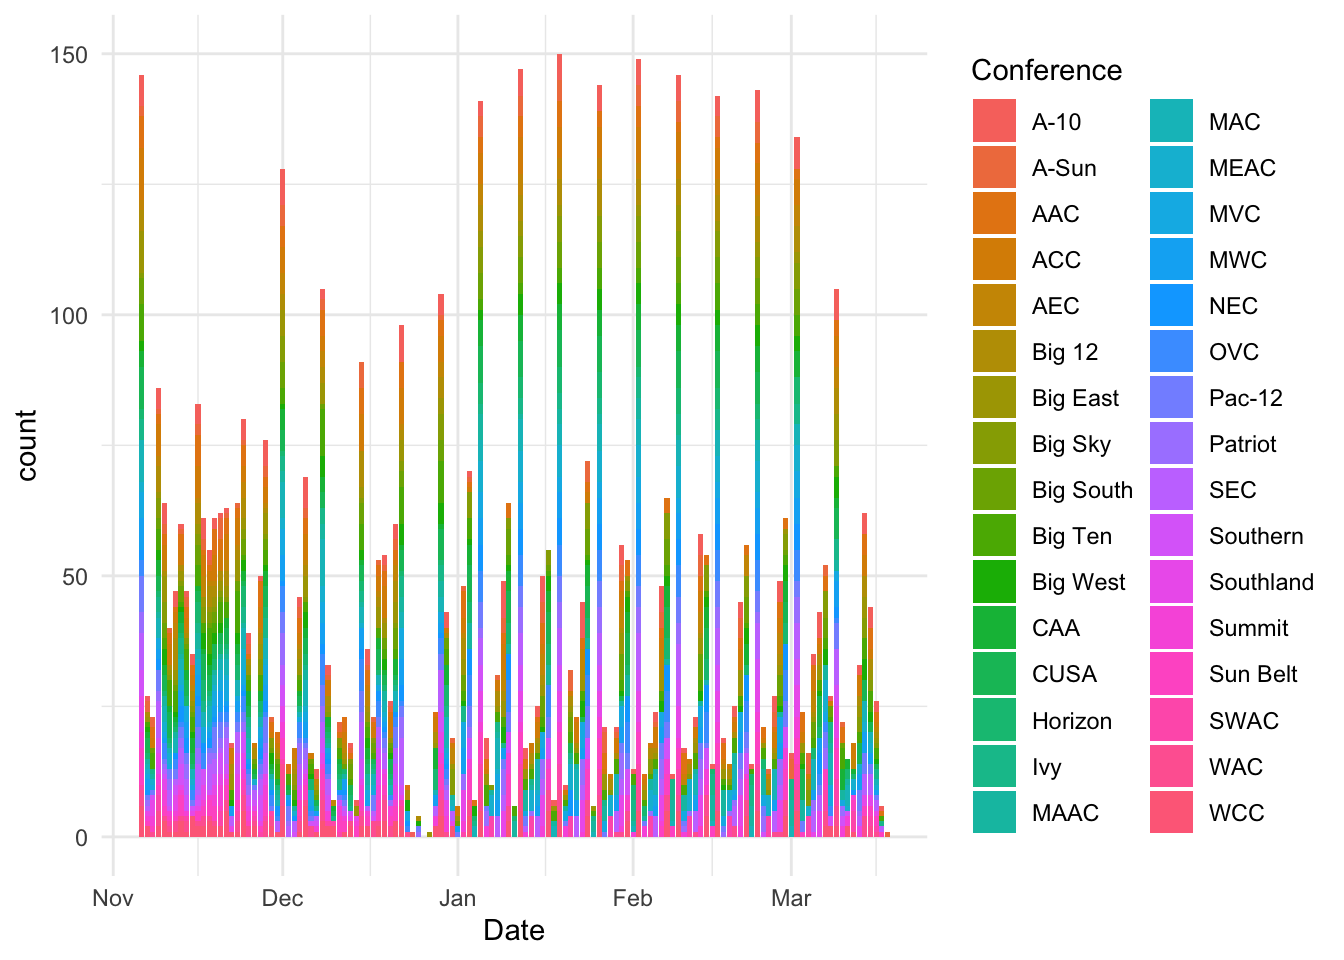
\includegraphics{datajournalism_files/figure-latex/unnamed-chunk-219-1.pdf}

This is going to be a story for months, if not years. So repeating this analysis is a must for a reporter covering the economy in Nebraska. We've set ourselves up to do this every week when the data comes out. We just open our notebook, go to Run \textgreater{} Restart R and Run All Chunks and sit back and watch as it does it all again.

Then we go report.

\hypertarget{the-state-vs-the-feds}{%
\section{The State vs the Feds}\label{the-state-vs-the-feds}}

As I write this, the state hasn't updated their data but the feds have, and the feds have more. The problem? It's a mess. And it's not automatable. So to get more data, you need to go to \href{https://oui.doleta.gov/unemploy/claims.asp}{the Department of Labor website} and fill out the form.

Select Spreadsheet, but know that it's a lie. If you try to load it using read\_excel, you'll get an error. Why? Because what is being downloaded is an HTML file. So you can use \texttt{rvest} to read and parse it.

However, that isn't so simple.

\begin{Shaded}
\begin{Highlighting}[]
\KeywordTok{library}\NormalTok{(rvest)}
\KeywordTok{library}\NormalTok{(lubridate)}
\end{Highlighting}
\end{Shaded}

First, read the file you downloaded. You'll need to add the \texttt{fill=TRUE} to html\_table() to solve a problem with some of the data.

\begin{Shaded}
\begin{Highlighting}[]
\NormalTok{claims <-}\StringTok{ }\KeywordTok{read_html}\NormalTok{(}\StringTok{"~/Downloads/r539cy.xls"}\NormalTok{) }\OperatorTok\StringTok{ }
\StringTok{  }\KeywordTok{html_nodes}\NormalTok{(}\StringTok{"table"}\NormalTok{) }\OperatorTok
\StringTok{  }\KeywordTok{html_table}\NormalTok{(}\DataTypeTok{fill=}\OtherTok{TRUE}\NormalTok{) }
\end{Highlighting}
\end{Shaded}

Similar to previous efforts, we get a list. The first element is a dataframe, so let's get that.

\begin{Shaded}
\begin{Highlighting}[]
\NormalTok{claims <-}\StringTok{ }\NormalTok{claims[[}\DecValTok{1}\NormalTok{]] }
\end{Highlighting}
\end{Shaded}

Now if you look at this data, you'll see that the header row is empty, and the header names are in the first row. Also, none of this data is formatted correctly. We need to fix that.

To do this, we're going to fix this in steps after we create a new dataframe called \texttt{cleanclaims}

\begin{enumerate}
\def\labelenumi{\arabic{enumi}.}
\tightlist
\item
  We'll remove empty columns.
\item
  We'll rename the columns with what they are, using \texttt{janitor} style naming conventions.
\item
  We'll filter out the old header row.
\item
  We'll mutate each field to format them correctly. The date columns will use \texttt{lubridate}'s \texttt{mdy} function. Numbers will use \texttt{readr}'s \texttt{parse\_number} function to solve the comma separator issue.
\end{enumerate}

\begin{Shaded}
\begin{Highlighting}[]
\NormalTok{cleanclaims <-}\StringTok{ }\NormalTok{claims }\OperatorTok\StringTok{ }
\StringTok{  }\KeywordTok{remove_empty}\NormalTok{(}\StringTok{"cols"}\NormalTok{) }\OperatorTok\StringTok{ }
\StringTok{  }\KeywordTok{rename}\NormalTok{(}\StringTok{"state"}\NormalTok{ =}\StringTok{ }\DecValTok{1}\NormalTok{, }\StringTok{"filed_week_ended"}\NormalTok{=}\StringTok{ }\DecValTok{2}\NormalTok{, }\StringTok{"initial_claims"}\NormalTok{=}\DecValTok{3}\NormalTok{, }\StringTok{"reflecting_week_ended"}\NormalTok{=}\DecValTok{4}\NormalTok{, }\StringTok{"continued_claims"}\NormalTok{=}\DecValTok{5}\NormalTok{, }\StringTok{"covered_employment"}\NormalTok{=}\DecValTok{6}\NormalTok{, }\StringTok{"insured_unemployment_rate"}\NormalTok{=}\DecValTok{7}\NormalTok{) }\OperatorTok
\StringTok{  }\KeywordTok{filter}\NormalTok{(state }\OperatorTok{!=}\StringTok{ "State"}\NormalTok{) }\OperatorTok\StringTok{ }
\StringTok{  }\KeywordTok{mutate}\NormalTok{(}\DataTypeTok{filed_week_ended =} \KeywordTok{mdy}\NormalTok{(filed_week_ended), }\DataTypeTok{initial_claims=}\KeywordTok{parse_number}\NormalTok{(initial_claims), }\DataTypeTok{reflecting_week_ended=}\KeywordTok{mdy}\NormalTok{(reflecting_week_ended), }\DataTypeTok{continued_claims=}\KeywordTok{parse_number}\NormalTok{(continued_claims), }\DataTypeTok{covered_employment=}\KeywordTok{parse_number}\NormalTok{(covered_employment), }\DataTypeTok{insured_unemployment_rate=}\KeywordTok{parse_number}\NormalTok{(insured_unemployment_rate))}
\end{Highlighting}
\end{Shaded}

If you open \texttt{cleanclaims}, you may notice something, depending on when you do this analysis:

\begin{Shaded}
\begin{Highlighting}[]
\NormalTok{cleanclaims }\OperatorTok\StringTok{ }\KeywordTok{arrange}\NormalTok{(}\KeywordTok{desc}\NormalTok{(filed_week_ended)) }\OperatorTok\StringTok{ }\KeywordTok{head}\NormalTok{()}
\end{Highlighting}
\end{Shaded}

\begin{verbatim}
##      state filed_week_ended initial_claims reflecting_week_ended
## 1 Nebraska       2020-03-14            795            2020-03-07
## 2 Nebraska       2020-03-07            501            2020-02-29
## 3 Nebraska       2020-02-29            502            2020-02-22
## 4 Nebraska       2020-02-22            493            2020-02-15
## 5 Nebraska       2020-02-15            537            2020-02-08
## 6 Nebraska       2020-02-08            675            2020-02-01
##   continued_claims covered_employment insured_unemployment_rate
## 1             5076             962725                      0.53
## 2             5581             962725                      0.58
## 3             6286             962725                      0.65
## 4             5780             962725                      0.60
## 5             5804             962725                      0.60
## 6             5693             962725                      0.59
\end{verbatim}

See it? The latest data isn't in there in my version. \href{https://www.dol.gov/sites/dolgov/files/OPA/newsreleases/ui-claims/20200510.pdf}{It's in a press release}.

So how do we add it? We use \texttt{add\_row} from the tidyverse (specifically the \texttt{tibble} library).

\begin{Shaded}
\begin{Highlighting}[]
\NormalTok{updatedcleanclaims <-}\StringTok{ }\NormalTok{cleanclaims }\OperatorTok\StringTok{ }\KeywordTok{add_row}\NormalTok{(}\DataTypeTok{state=}\StringTok{"Nebraska"}\NormalTok{, }\DataTypeTok{filed_week_ended=}\KeywordTok{as.Date}\NormalTok{(}\StringTok{"2020-03-21"}\NormalTok{), }\DataTypeTok{initial_claims=}\DecValTok{15688}\NormalTok{, }\DataTypeTok{reflecting_week_ended=}\KeywordTok{as.Date}\NormalTok{(}\StringTok{"2020-03-14"}\NormalTok{))}
\end{Highlighting}
\end{Shaded}

Now we can repeat the analysis from above.

First we rank.

\begin{Shaded}
\begin{Highlighting}[]
\NormalTok{fedranked <-}\StringTok{ }\NormalTok{updatedcleanclaims }\OperatorTok\StringTok{ }\KeywordTok{mutate}\NormalTok{(}\DataTypeTok{Rank =} \KeywordTok{min_rank}\NormalTok{(}\KeywordTok{desc}\NormalTok{(initial_claims))) }\OperatorTok\StringTok{ }\KeywordTok{arrange}\NormalTok{(}\KeywordTok{desc}\NormalTok{(filed_week_ended))}
\end{Highlighting}
\end{Shaded}

We get the latest week.

\begin{Shaded}
\begin{Highlighting}[]
\NormalTok{fedlatest <-}\StringTok{ }\NormalTok{fedranked }\OperatorTok\StringTok{ }\KeywordTok{slice}\NormalTok{(}\DecValTok{1}\NormalTok{)}
\end{Highlighting}
\end{Shaded}

And we make the graphic.

\begin{Shaded}
\begin{Highlighting}[]
\KeywordTok{ggplot}\NormalTok{() }\OperatorTok{+}\StringTok{ }
\StringTok{  }\KeywordTok{geom_line}\NormalTok{(}\DataTypeTok{data=}\NormalTok{fedranked, }\KeywordTok{aes}\NormalTok{(}\DataTypeTok{x=}\NormalTok{filed_week_ended, }\DataTypeTok{y=}\NormalTok{initial_claims, }\DataTypeTok{group=}\DecValTok{1}\NormalTok{)) }\OperatorTok{+}
\StringTok{  }\KeywordTok{geom_point}\NormalTok{(}\DataTypeTok{data=}\NormalTok{fedlatest, }\KeywordTok{aes}\NormalTok{(}\DataTypeTok{x=}\NormalTok{filed_week_ended, }\DataTypeTok{y=}\NormalTok{initial_claims)) }\OperatorTok{+}\StringTok{ }
\StringTok{  }\KeywordTok{geom_text}\NormalTok{(}\DataTypeTok{data=}\NormalTok{fedlatest, }\KeywordTok{aes}\NormalTok{(}\DataTypeTok{x=}\NormalTok{filed_week_ended}\DecValTok{-200}\NormalTok{, }\DataTypeTok{y=}\NormalTok{initial_claims }\OperatorTok{+}\StringTok{ }\DecValTok{500}\NormalTok{, }\DataTypeTok{label=}\StringTok{"15,668"}\NormalTok{)) }\OperatorTok{+}\StringTok{ }
\StringTok{  }\KeywordTok{geom_smooth}\NormalTok{(}\DataTypeTok{data=}\NormalTok{fedranked, }\KeywordTok{aes}\NormalTok{(}\DataTypeTok{x=}\NormalTok{filed_week_ended, }\DataTypeTok{y=}\NormalTok{initial_claims), }\DataTypeTok{method=}\NormalTok{loess, }\DataTypeTok{se=}\OtherTok{FALSE}\NormalTok{) }\OperatorTok{+}\StringTok{ }
\StringTok{  }\KeywordTok{labs}\NormalTok{(}\DataTypeTok{title=}\StringTok{"A record for jobless claims in Nebraska"}\NormalTok{, }\DataTypeTok{subtitle=}\StringTok{"Applications for unemployment jumped 1,871 percent from the week ending March 14 to the 21st. The worst is yet to come."}\NormalTok{, }\DataTypeTok{x=}\StringTok{"Date"}\NormalTok{, }\DataTypeTok{y=}\StringTok{"Claims"}\NormalTok{, }\DataTypeTok{caption =} \StringTok{"Source: US Dept. of Labor  |  Graphic by Matt Waite"}\NormalTok{) }\OperatorTok{+}
\StringTok{  }\KeywordTok{theme_minimal}\NormalTok{() }\OperatorTok{+}\StringTok{ }
\StringTok{  }\KeywordTok{theme}\NormalTok{(}
    \DataTypeTok{plot.title =} \KeywordTok{element_text}\NormalTok{(}\DataTypeTok{size =} \DecValTok{16}\NormalTok{, }\DataTypeTok{face =} \StringTok{"bold"}\NormalTok{),}
    \DataTypeTok{axis.title =} \KeywordTok{element_text}\NormalTok{(}\DataTypeTok{size =} \DecValTok{8}\NormalTok{), }
    \DataTypeTok{plot.subtitle =} \KeywordTok{element_text}\NormalTok{(}\DataTypeTok{size=}\DecValTok{10}\NormalTok{), }
    \DataTypeTok{panel.grid.minor =} \KeywordTok{element_blank}\NormalTok{()}
\NormalTok{    )}
\end{Highlighting}
\end{Shaded}

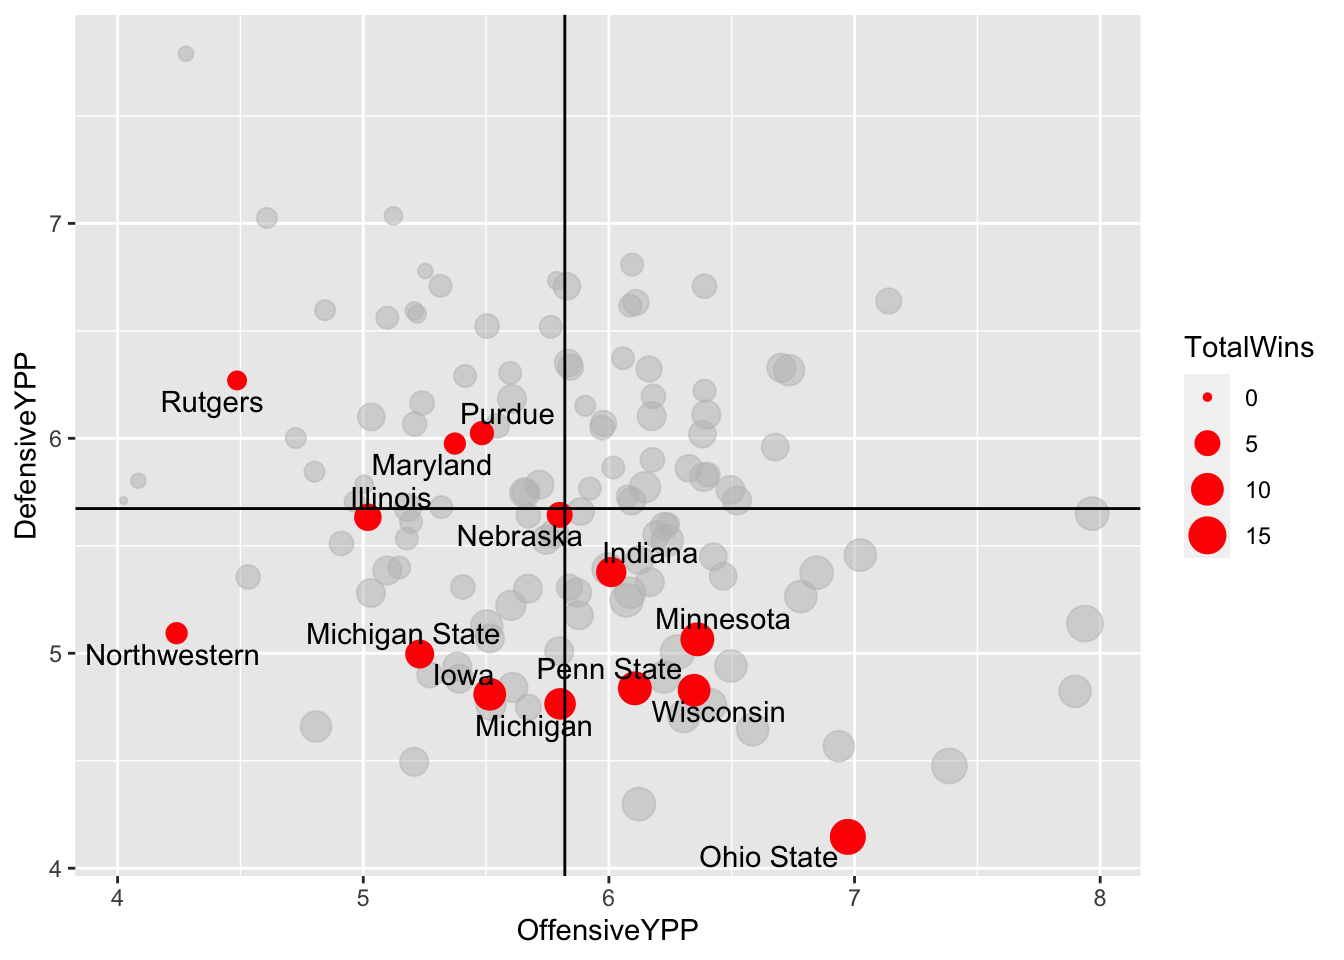
\includegraphics{datajournalism_files/figure-latex/unnamed-chunk-228-1.pdf}

\hypertarget{automating-geographic-analysis}{%
\chapter{Automating geographic analysis}\label{automating-geographic-analysis}}

One thing that has been very apparent with the coronavirus outbreak is that this is a very geographic story. Where cases are being found and how fast is news, so it would be a good idea for us to have updating maps. But to have that, we need to have updating data.

Good news.

The New York Times is making the data behind \href{https://www.nytimes.com/interactive/2020/us/coronavirus-us-cases.html}{their interactive trackers} \href{https://github.com/nytimes/covid-19-data}{available to others for free}.

So we have a constantly updating data stream on Github, so that means we can make this work.

Let's get our libraries first:

\begin{Shaded}
\begin{Highlighting}[]
\KeywordTok{library}\NormalTok{(tidyverse)}
\KeywordTok{library}\NormalTok{(sf)}
\end{Highlighting}
\end{Shaded}

We can use \texttt{read\_csv} to read a URL if that URL is to a csv file. And Github just happens to provide a direct link to the CSV of county COVID-19 reports. Here's what that looks like:

\begin{Shaded}
\begin{Highlighting}[]
\NormalTok{covid <-}\StringTok{ }\KeywordTok{read_csv}\NormalTok{(}\StringTok{"https://raw.githubusercontent.com/nytimes/covid-19-data/master/us-counties.csv"}\NormalTok{)}
\end{Highlighting}
\end{Shaded}

\begin{verbatim}
## Parsed with column specification:
## cols(
##   date = col_date(format = ""),
##   county = col_character(),
##   state = col_character(),
##   fips = col_character(),
##   cases = col_double(),
##   deaths = col_double()
## )
\end{verbatim}

Let's look at what the New York Times is providing us:

\begin{Shaded}
\begin{Highlighting}[]
\KeywordTok{head}\NormalTok{(covid)}
\end{Highlighting}
\end{Shaded}

\begin{verbatim}
## # A tibble: 6 x 6
##   date       county    state      fips  cases deaths
##   <date>     <chr>     <chr>      <chr> <dbl>  <dbl>
## 1 2020-01-21 Snohomish Washington 53061     1      0
## 2 2020-01-22 Snohomish Washington 53061     1      0
## 3 2020-01-23 Snohomish Washington 53061     1      0
## 4 2020-01-24 Cook      Illinois   17031     1      0
## 5 2020-01-24 Snohomish Washington 53061     1      0
## 6 2020-01-25 Orange    California 06059     1      0
\end{verbatim}

If you look, we have a county and a date -- how many cases are reported in that county on that day. That means we can do some interesting progression charts.

Let's filter out Nebraska first.

\begin{Shaded}
\begin{Highlighting}[]
\NormalTok{nebraska <-}\StringTok{ }\NormalTok{covid }\OperatorTok\StringTok{ }\KeywordTok{filter}\NormalTok{(state }\OperatorTok{==}\StringTok{ "Nebraska"}\NormalTok{)}
\end{Highlighting}
\end{Shaded}

And we can create line chart like this:

\begin{Shaded}
\begin{Highlighting}[]
\KeywordTok{ggplot}\NormalTok{() }\OperatorTok{+}\StringTok{ }\KeywordTok{geom_line}\NormalTok{(}\DataTypeTok{data=}\NormalTok{nebraska, }\KeywordTok{aes}\NormalTok{(}\DataTypeTok{x=}\NormalTok{date, }\DataTypeTok{y=}\NormalTok{cases, }\DataTypeTok{group=}\NormalTok{county, }\DataTypeTok{color=}\NormalTok{county))}
\end{Highlighting}
\end{Shaded}

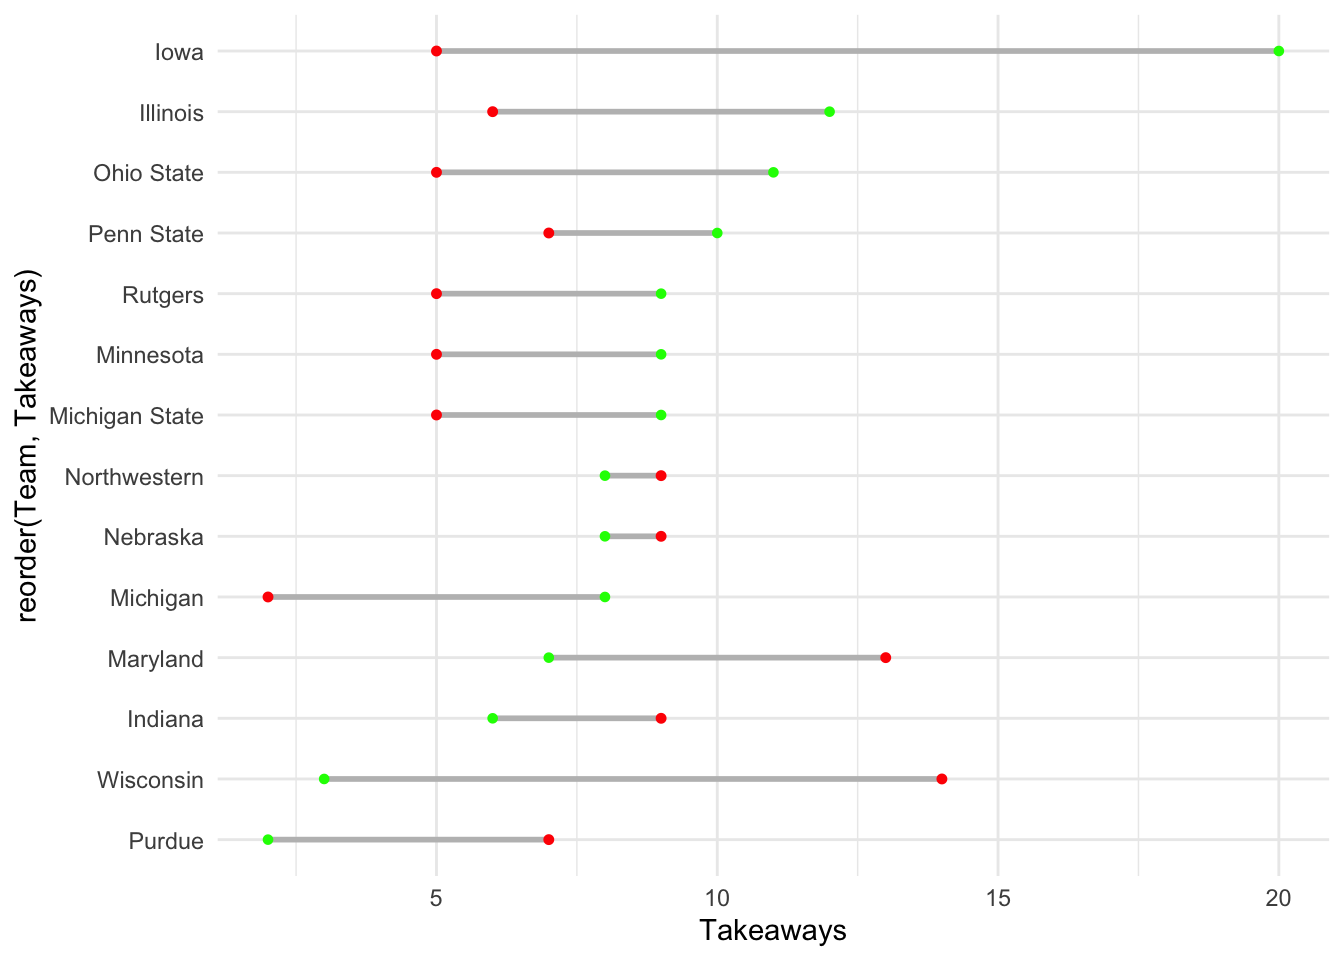
\includegraphics{datajournalism_files/figure-latex/unnamed-chunk-233-1.pdf}

The little county on the bottom that curves sharply up? That's my home county, Washington County. One day of this writing, they added 10 cases in one day in one nursing home. Grim stuff.

The curve you see for Douglas County is a classic exponential curve. Because the number of cases here are small, we can get away with it for a little while. But when looking at much larger places, you'd use a log scale. \href{https://www.ft.com/video/9a72a9d4-8db1-4615-8333-4b73ae3ddff8}{YOU REALLY SHOULD WATCH THIS}. You've no doubt seen the Financial Times coronavirus trajectory tracker. Hear why they are using a log scale. And here's what our chart looks like with it. Note the y-axis scale.

\begin{Shaded}
\begin{Highlighting}[]
\KeywordTok{ggplot}\NormalTok{() }\OperatorTok{+}\StringTok{ }\KeywordTok{geom_line}\NormalTok{(}\DataTypeTok{data=}\NormalTok{nebraska, }\KeywordTok{aes}\NormalTok{(}\DataTypeTok{x=}\NormalTok{date, }\DataTypeTok{y=}\NormalTok{cases, }\DataTypeTok{group=}\NormalTok{county, }\DataTypeTok{color=}\NormalTok{county)) }\OperatorTok{+}\StringTok{ }\KeywordTok{scale_y_continuous}\NormalTok{(}\DataTypeTok{trans=}\StringTok{"log10"}\NormalTok{)}
\end{Highlighting}
\end{Shaded}

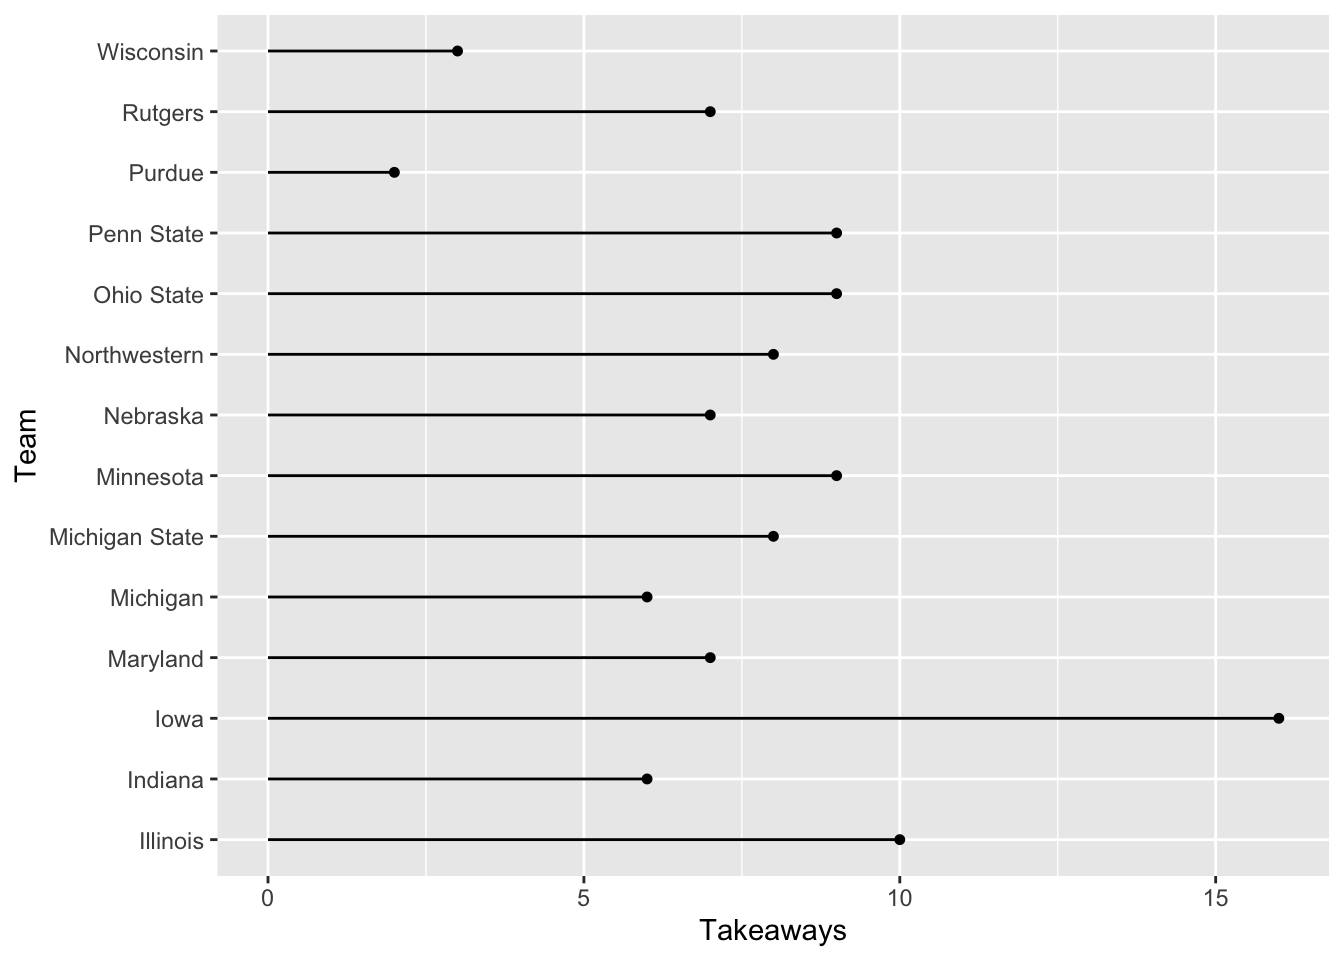
\includegraphics{datajournalism_files/figure-latex/unnamed-chunk-234-1.pdf}

\hypertarget{mapping-continuously}{%
\section{Mapping continuously}\label{mapping-continuously}}

But for a map, we can't have multiple days. We need a single day. Ideally, it would be the most recent date. We can get it using the \texttt{max} function.

\begin{Shaded}
\begin{Highlighting}[]
\NormalTok{current <-}\StringTok{ }\NormalTok{nebraska }\OperatorTok\StringTok{ }\KeywordTok{summarize}\NormalTok{(}\KeywordTok{max}\NormalTok{(date))}
\end{Highlighting}
\end{Shaded}

That will give us the most recent date in Nebraska in a variable called \texttt{current}. And now we can filter the most recent data for Nebraska, regardless of when this runs.

I'm adding one piece to the end to make joining this to a map easier and just renaming fips to GEOID, because they are identical in both datasets and can be used for joining.

\begin{Shaded}
\begin{Highlighting}[]
\NormalTok{nebraskacurrent <-}\StringTok{ }\NormalTok{nebraska }\OperatorTok\StringTok{ }\KeywordTok{filter}\NormalTok{(date }\OperatorTok{==}\StringTok{ }\NormalTok{current[[}\DecValTok{1}\NormalTok{]]) }\OperatorTok\StringTok{ }\KeywordTok{rename}\NormalTok{(}\DataTypeTok{GEOID =}\NormalTok{ fips)}
\end{Highlighting}
\end{Shaded}

Now we can read in our counties map layer.

\begin{Shaded}
\begin{Highlighting}[]
\NormalTok{counties <-}\StringTok{ }\KeywordTok{st_read}\NormalTok{(}\StringTok{"data/cb_2018_us_county_5m/cb_2018_us_county_5m.shp"}\NormalTok{)}
\end{Highlighting}
\end{Shaded}

\begin{verbatim}
## Reading layer `cb_2018_us_county_5m' from data source `/Users/mwaite3/Box/BookProjects/DataJournalismWithR/data/cb_2018_us_county_5m/cb_2018_us_county_5m.shp' using driver `ESRI Shapefile'
## Simple feature collection with 3233 features and 9 fields
## geometry type:  MULTIPOLYGON
## dimension:      XY
## bbox:           xmin: -179.1473 ymin: -14.55255 xmax: 179.7785 ymax: 71.35256
## epsg (SRID):    4269
## proj4string:    +proj=longlat +ellps=GRS80 +towgs84=0,0,0,0,0,0,0 +no_defs
\end{verbatim}

And join the two together.

\begin{Shaded}
\begin{Highlighting}[]
\NormalTok{counties <-}\StringTok{ }\NormalTok{counties }\OperatorTok\StringTok{ }\KeywordTok{left_join}\NormalTok{(nebraskacurrent)}
\end{Highlighting}
\end{Shaded}

\begin{verbatim}
## Joining, by = "GEOID"
\end{verbatim}

\begin{verbatim}
## Warning: Column `GEOID` joining factor and character vector, coercing into
## character vector
\end{verbatim}

Since we have every county in the United States in our counties map layer, we can filter just Nebraska like this:

\begin{Shaded}
\begin{Highlighting}[]
\NormalTok{necounties <-}\StringTok{ }\NormalTok{counties }\OperatorTok\StringTok{ }\KeywordTok{filter}\NormalTok{(STATEFP }\OperatorTok{==}\StringTok{ }\DecValTok{31}\NormalTok{)}
\end{Highlighting}
\end{Shaded}

So now, we have a geographic dataframe that has both the county shapes and the number of cases in the most recent data update. We just need to see it now:

\begin{Shaded}
\begin{Highlighting}[]
\KeywordTok{ggplot}\NormalTok{() }\OperatorTok{+}\StringTok{ }
\StringTok{  }\KeywordTok{geom_sf}\NormalTok{(}\DataTypeTok{data=}\NormalTok{necounties, }\KeywordTok{aes}\NormalTok{(}\DataTypeTok{fill=}\NormalTok{cases)) }\OperatorTok{+}\StringTok{ }
\StringTok{  }\KeywordTok{scale_fill_viridis_c}\NormalTok{(}\DataTypeTok{option =} \StringTok{"plasma"}\NormalTok{, }\DataTypeTok{trans =} \StringTok{"sqrt"}\NormalTok{) }\OperatorTok{+}\StringTok{ }
\StringTok{  }\KeywordTok{theme_void}\NormalTok{() }\OperatorTok{+}\StringTok{ }
\StringTok{  }\KeywordTok{labs}\NormalTok{(}\DataTypeTok{title =} \KeywordTok{paste}\NormalTok{(}\StringTok{"COVID-19 cases as of "}\NormalTok{, current[[}\DecValTok{1}\NormalTok{]], }\DataTypeTok{sep=}\StringTok{""}\NormalTok{))}
\end{Highlighting}
\end{Shaded}

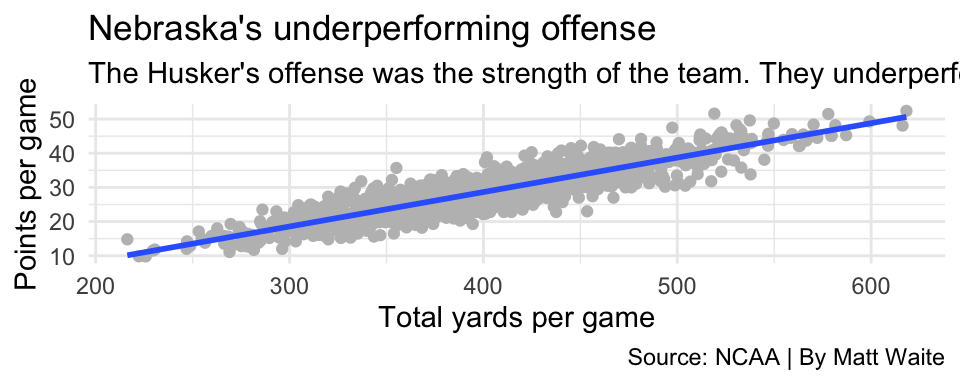
\includegraphics{datajournalism_files/figure-latex/unnamed-chunk-240-1.pdf}

As it stands, we can run this every day and get an up-to-date map.

\end{document}
